
% Default to the notebook output style

    


% Inherit from the specified cell style.




    
\documentclass[11pt, a4paper , landscape]{article}

    
    
    \usepackage[T1]{fontenc}
    % Nicer default font (+ math font) than Computer Modern for most use cases
    \usepackage{mathpazo}

    % Basic figure setup, for now with no caption control since it's done
    % automatically by Pandoc (which extracts ![](path) syntax from Markdown).
    \usepackage{graphicx}
    % We will generate all images so they have a width \maxwidth. This means
    % that they will get their normal width if they fit onto the page, but
    % are scaled down if they would overflow the margins.
    \makeatletter
    \def\maxwidth{\ifdim\Gin@nat@width>\linewidth\linewidth
    \else\Gin@nat@width\fi}
    \makeatother
    \let\Oldincludegraphics\includegraphics
    % Set max figure width to be 80% of text width, for now hardcoded.
    \renewcommand{\includegraphics}[1]{\Oldincludegraphics[width=.8\maxwidth]{#1}}
    % Ensure that by default, figures have no caption (until we provide a
    % proper Figure object with a Caption API and a way to capture that
    % in the conversion process - todo).
    \usepackage{caption}
    \DeclareCaptionLabelFormat{nolabel}{}
    \captionsetup{labelformat=nolabel}

    \usepackage{adjustbox} % Used to constrain images to a maximum size 
    \usepackage{xcolor} % Allow colors to be defined
    \usepackage{enumerate} % Needed for markdown enumerations to work
    \usepackage{geometry} % Used to adjust the document margins
    \usepackage{amsmath} % Equations
    \usepackage{amssymb} % Equations
    \usepackage{textcomp} % defines textquotesingle
    % Hack from http://tex.stackexchange.com/a/47451/13684:
    \AtBeginDocument{%
        \def\PYZsq{\textquotesingle}% Upright quotes in Pygmentized code
    }
    \usepackage{upquote} % Upright quotes for verbatim code
    \usepackage{eurosym} % defines \euro
    \usepackage[mathletters]{ucs} % Extended unicode (utf-8) support
    \usepackage[utf8x]{inputenc} % Allow utf-8 characters in the tex document
    \usepackage{fancyvrb} % verbatim replacement that allows latex
    \usepackage{grffile} % extends the file name processing of package graphics 
                         % to support a larger range 
    % The hyperref package gives us a pdf with properly built
    % internal navigation ('pdf bookmarks' for the table of contents,
    % internal cross-reference links, web links for URLs, etc.)
    \usepackage{hyperref}
    \usepackage{longtable} % longtable support required by pandoc >1.10
    \usepackage{booktabs}  % table support for pandoc > 1.12.2
    \usepackage[inline]{enumitem} % IRkernel/repr support (it uses the enumerate* environment)
    \usepackage[normalem]{ulem} % ulem is needed to support strikethroughs (\sout)
                                % normalem makes italics be italics, not underlines
    \usepackage{mathrsfs}
    

    
    
    % Colors for the hyperref package
    \definecolor{urlcolor}{rgb}{0,.145,.698}
    \definecolor{linkcolor}{rgb}{.71,0.21,0.01}
    \definecolor{citecolor}{rgb}{.12,.54,.11}

    % ANSI colors
    \definecolor{ansi-black}{HTML}{3E424D}
    \definecolor{ansi-black-intense}{HTML}{282C36}
    \definecolor{ansi-red}{HTML}{E75C58}
    \definecolor{ansi-red-intense}{HTML}{B22B31}
    \definecolor{ansi-green}{HTML}{00A250}
    \definecolor{ansi-green-intense}{HTML}{007427}
    \definecolor{ansi-yellow}{HTML}{DDB62B}
    \definecolor{ansi-yellow-intense}{HTML}{B27D12}
    \definecolor{ansi-blue}{HTML}{208FFB}
    \definecolor{ansi-blue-intense}{HTML}{0065CA}
    \definecolor{ansi-magenta}{HTML}{D160C4}
    \definecolor{ansi-magenta-intense}{HTML}{A03196}
    \definecolor{ansi-cyan}{HTML}{60C6C8}
    \definecolor{ansi-cyan-intense}{HTML}{258F8F}
    \definecolor{ansi-white}{HTML}{C5C1B4}
    \definecolor{ansi-white-intense}{HTML}{A1A6B2}
    \definecolor{ansi-default-inverse-fg}{HTML}{FFFFFF}
    \definecolor{ansi-default-inverse-bg}{HTML}{000000}

    % commands and environments needed by pandoc snippets
    % extracted from the output of `pandoc -s`
    \providecommand{\tightlist}{%
      \setlength{\itemsep}{0pt}\setlength{\parskip}{0pt}}
    \DefineVerbatimEnvironment{Highlighting}{Verbatim}{commandchars=\\\{\}}
    % Add ',fontsize=\small' for more characters per line
    \newenvironment{Shaded}{}{}
    \newcommand{\KeywordTok}[1]{\textcolor[rgb]{0.00,0.44,0.13}{\textbf{{#1}}}}
    \newcommand{\DataTypeTok}[1]{\textcolor[rgb]{0.56,0.13,0.00}{{#1}}}
    \newcommand{\DecValTok}[1]{\textcolor[rgb]{0.25,0.63,0.44}{{#1}}}
    \newcommand{\BaseNTok}[1]{\textcolor[rgb]{0.25,0.63,0.44}{{#1}}}
    \newcommand{\FloatTok}[1]{\textcolor[rgb]{0.25,0.63,0.44}{{#1}}}
    \newcommand{\CharTok}[1]{\textcolor[rgb]{0.25,0.44,0.63}{{#1}}}
    \newcommand{\StringTok}[1]{\textcolor[rgb]{0.25,0.44,0.63}{{#1}}}
    \newcommand{\CommentTok}[1]{\textcolor[rgb]{0.38,0.63,0.69}{\textit{{#1}}}}
    \newcommand{\OtherTok}[1]{\textcolor[rgb]{0.00,0.44,0.13}{{#1}}}
    \newcommand{\AlertTok}[1]{\textcolor[rgb]{1.00,0.00,0.00}{\textbf{{#1}}}}
    \newcommand{\FunctionTok}[1]{\textcolor[rgb]{0.02,0.16,0.49}{{#1}}}
    \newcommand{\RegionMarkerTok}[1]{{#1}}
    \newcommand{\ErrorTok}[1]{\textcolor[rgb]{1.00,0.00,0.00}{\textbf{{#1}}}}
    \newcommand{\NormalTok}[1]{{#1}}
    
    % Additional commands for more recent versions of Pandoc
    \newcommand{\ConstantTok}[1]{\textcolor[rgb]{0.53,0.00,0.00}{{#1}}}
    \newcommand{\SpecialCharTok}[1]{\textcolor[rgb]{0.25,0.44,0.63}{{#1}}}
    \newcommand{\VerbatimStringTok}[1]{\textcolor[rgb]{0.25,0.44,0.63}{{#1}}}
    \newcommand{\SpecialStringTok}[1]{\textcolor[rgb]{0.73,0.40,0.53}{{#1}}}
    \newcommand{\ImportTok}[1]{{#1}}
    \newcommand{\DocumentationTok}[1]{\textcolor[rgb]{0.73,0.13,0.13}{\textit{{#1}}}}
    \newcommand{\AnnotationTok}[1]{\textcolor[rgb]{0.38,0.63,0.69}{\textbf{\textit{{#1}}}}}
    \newcommand{\CommentVarTok}[1]{\textcolor[rgb]{0.38,0.63,0.69}{\textbf{\textit{{#1}}}}}
    \newcommand{\VariableTok}[1]{\textcolor[rgb]{0.10,0.09,0.49}{{#1}}}
    \newcommand{\ControlFlowTok}[1]{\textcolor[rgb]{0.00,0.44,0.13}{\textbf{{#1}}}}
    \newcommand{\OperatorTok}[1]{\textcolor[rgb]{0.40,0.40,0.40}{{#1}}}
    \newcommand{\BuiltInTok}[1]{{#1}}
    \newcommand{\ExtensionTok}[1]{{#1}}
    \newcommand{\PreprocessorTok}[1]{\textcolor[rgb]{0.74,0.48,0.00}{{#1}}}
    \newcommand{\AttributeTok}[1]{\textcolor[rgb]{0.49,0.56,0.16}{{#1}}}
    \newcommand{\InformationTok}[1]{\textcolor[rgb]{0.38,0.63,0.69}{\textbf{\textit{{#1}}}}}
    \newcommand{\WarningTok}[1]{\textcolor[rgb]{0.38,0.63,0.69}{\textbf{\textit{{#1}}}}}
    
    
    % Define a nice break command that doesn't care if a line doesn't already
    % exist.
    \def\br{\hspace*{\fill} \\* }
    % Math Jax compatibility definitions
    \def\gt{>}
    \def\lt{<}
    \let\Oldtex\TeX
    \let\Oldlatex\LaTeX
    \renewcommand{\TeX}{\textrm{\Oldtex}}
    \renewcommand{\LaTeX}{\textrm{\Oldlatex}}
    % Document parameters
    % Document title
    \title{ House Prices: Advanced Regression Techniques }
    
    
    
    
    

    % Pygments definitions
    
\makeatletter
\def\PY@reset{\let\PY@it=\relax \let\PY@bf=\relax%
    \let\PY@ul=\relax \let\PY@tc=\relax%
    \let\PY@bc=\relax \let\PY@ff=\relax}
\def\PY@tok#1{\csname PY@tok@#1\endcsname}
\def\PY@toks#1+{\ifx\relax#1\empty\else%
    \PY@tok{#1}\expandafter\PY@toks\fi}
\def\PY@do#1{\PY@bc{\PY@tc{\PY@ul{%
    \PY@it{\PY@bf{\PY@ff{#1}}}}}}}
\def\PY#1#2{\PY@reset\PY@toks#1+\relax+\PY@do{#2}}

\expandafter\def\csname PY@tok@w\endcsname{\def\PY@tc##1{\textcolor[rgb]{0.73,0.73,0.73}{##1}}}
\expandafter\def\csname PY@tok@c\endcsname{\let\PY@it=\textit\def\PY@tc##1{\textcolor[rgb]{0.25,0.50,0.50}{##1}}}
\expandafter\def\csname PY@tok@cp\endcsname{\def\PY@tc##1{\textcolor[rgb]{0.74,0.48,0.00}{##1}}}
\expandafter\def\csname PY@tok@k\endcsname{\let\PY@bf=\textbf\def\PY@tc##1{\textcolor[rgb]{0.00,0.50,0.00}{##1}}}
\expandafter\def\csname PY@tok@kp\endcsname{\def\PY@tc##1{\textcolor[rgb]{0.00,0.50,0.00}{##1}}}
\expandafter\def\csname PY@tok@kt\endcsname{\def\PY@tc##1{\textcolor[rgb]{0.69,0.00,0.25}{##1}}}
\expandafter\def\csname PY@tok@o\endcsname{\def\PY@tc##1{\textcolor[rgb]{0.40,0.40,0.40}{##1}}}
\expandafter\def\csname PY@tok@ow\endcsname{\let\PY@bf=\textbf\def\PY@tc##1{\textcolor[rgb]{0.67,0.13,1.00}{##1}}}
\expandafter\def\csname PY@tok@nb\endcsname{\def\PY@tc##1{\textcolor[rgb]{0.00,0.50,0.00}{##1}}}
\expandafter\def\csname PY@tok@nf\endcsname{\def\PY@tc##1{\textcolor[rgb]{0.00,0.00,1.00}{##1}}}
\expandafter\def\csname PY@tok@nc\endcsname{\let\PY@bf=\textbf\def\PY@tc##1{\textcolor[rgb]{0.00,0.00,1.00}{##1}}}
\expandafter\def\csname PY@tok@nn\endcsname{\let\PY@bf=\textbf\def\PY@tc##1{\textcolor[rgb]{0.00,0.00,1.00}{##1}}}
\expandafter\def\csname PY@tok@ne\endcsname{\let\PY@bf=\textbf\def\PY@tc##1{\textcolor[rgb]{0.82,0.25,0.23}{##1}}}
\expandafter\def\csname PY@tok@nv\endcsname{\def\PY@tc##1{\textcolor[rgb]{0.10,0.09,0.49}{##1}}}
\expandafter\def\csname PY@tok@no\endcsname{\def\PY@tc##1{\textcolor[rgb]{0.53,0.00,0.00}{##1}}}
\expandafter\def\csname PY@tok@nl\endcsname{\def\PY@tc##1{\textcolor[rgb]{0.63,0.63,0.00}{##1}}}
\expandafter\def\csname PY@tok@ni\endcsname{\let\PY@bf=\textbf\def\PY@tc##1{\textcolor[rgb]{0.60,0.60,0.60}{##1}}}
\expandafter\def\csname PY@tok@na\endcsname{\def\PY@tc##1{\textcolor[rgb]{0.49,0.56,0.16}{##1}}}
\expandafter\def\csname PY@tok@nt\endcsname{\let\PY@bf=\textbf\def\PY@tc##1{\textcolor[rgb]{0.00,0.50,0.00}{##1}}}
\expandafter\def\csname PY@tok@nd\endcsname{\def\PY@tc##1{\textcolor[rgb]{0.67,0.13,1.00}{##1}}}
\expandafter\def\csname PY@tok@s\endcsname{\def\PY@tc##1{\textcolor[rgb]{0.73,0.13,0.13}{##1}}}
\expandafter\def\csname PY@tok@sd\endcsname{\let\PY@it=\textit\def\PY@tc##1{\textcolor[rgb]{0.73,0.13,0.13}{##1}}}
\expandafter\def\csname PY@tok@si\endcsname{\let\PY@bf=\textbf\def\PY@tc##1{\textcolor[rgb]{0.73,0.40,0.53}{##1}}}
\expandafter\def\csname PY@tok@se\endcsname{\let\PY@bf=\textbf\def\PY@tc##1{\textcolor[rgb]{0.73,0.40,0.13}{##1}}}
\expandafter\def\csname PY@tok@sr\endcsname{\def\PY@tc##1{\textcolor[rgb]{0.73,0.40,0.53}{##1}}}
\expandafter\def\csname PY@tok@ss\endcsname{\def\PY@tc##1{\textcolor[rgb]{0.10,0.09,0.49}{##1}}}
\expandafter\def\csname PY@tok@sx\endcsname{\def\PY@tc##1{\textcolor[rgb]{0.00,0.50,0.00}{##1}}}
\expandafter\def\csname PY@tok@m\endcsname{\def\PY@tc##1{\textcolor[rgb]{0.40,0.40,0.40}{##1}}}
\expandafter\def\csname PY@tok@gh\endcsname{\let\PY@bf=\textbf\def\PY@tc##1{\textcolor[rgb]{0.00,0.00,0.50}{##1}}}
\expandafter\def\csname PY@tok@gu\endcsname{\let\PY@bf=\textbf\def\PY@tc##1{\textcolor[rgb]{0.50,0.00,0.50}{##1}}}
\expandafter\def\csname PY@tok@gd\endcsname{\def\PY@tc##1{\textcolor[rgb]{0.63,0.00,0.00}{##1}}}
\expandafter\def\csname PY@tok@gi\endcsname{\def\PY@tc##1{\textcolor[rgb]{0.00,0.63,0.00}{##1}}}
\expandafter\def\csname PY@tok@gr\endcsname{\def\PY@tc##1{\textcolor[rgb]{1.00,0.00,0.00}{##1}}}
\expandafter\def\csname PY@tok@ge\endcsname{\let\PY@it=\textit}
\expandafter\def\csname PY@tok@gs\endcsname{\let\PY@bf=\textbf}
\expandafter\def\csname PY@tok@gp\endcsname{\let\PY@bf=\textbf\def\PY@tc##1{\textcolor[rgb]{0.00,0.00,0.50}{##1}}}
\expandafter\def\csname PY@tok@go\endcsname{\def\PY@tc##1{\textcolor[rgb]{0.53,0.53,0.53}{##1}}}
\expandafter\def\csname PY@tok@gt\endcsname{\def\PY@tc##1{\textcolor[rgb]{0.00,0.27,0.87}{##1}}}
\expandafter\def\csname PY@tok@err\endcsname{\def\PY@bc##1{\setlength{\fboxsep}{0pt}\fcolorbox[rgb]{1.00,0.00,0.00}{1,1,1}{\strut ##1}}}
\expandafter\def\csname PY@tok@kc\endcsname{\let\PY@bf=\textbf\def\PY@tc##1{\textcolor[rgb]{0.00,0.50,0.00}{##1}}}
\expandafter\def\csname PY@tok@kd\endcsname{\let\PY@bf=\textbf\def\PY@tc##1{\textcolor[rgb]{0.00,0.50,0.00}{##1}}}
\expandafter\def\csname PY@tok@kn\endcsname{\let\PY@bf=\textbf\def\PY@tc##1{\textcolor[rgb]{0.00,0.50,0.00}{##1}}}
\expandafter\def\csname PY@tok@kr\endcsname{\let\PY@bf=\textbf\def\PY@tc##1{\textcolor[rgb]{0.00,0.50,0.00}{##1}}}
\expandafter\def\csname PY@tok@bp\endcsname{\def\PY@tc##1{\textcolor[rgb]{0.00,0.50,0.00}{##1}}}
\expandafter\def\csname PY@tok@fm\endcsname{\def\PY@tc##1{\textcolor[rgb]{0.00,0.00,1.00}{##1}}}
\expandafter\def\csname PY@tok@vc\endcsname{\def\PY@tc##1{\textcolor[rgb]{0.10,0.09,0.49}{##1}}}
\expandafter\def\csname PY@tok@vg\endcsname{\def\PY@tc##1{\textcolor[rgb]{0.10,0.09,0.49}{##1}}}
\expandafter\def\csname PY@tok@vi\endcsname{\def\PY@tc##1{\textcolor[rgb]{0.10,0.09,0.49}{##1}}}
\expandafter\def\csname PY@tok@vm\endcsname{\def\PY@tc##1{\textcolor[rgb]{0.10,0.09,0.49}{##1}}}
\expandafter\def\csname PY@tok@sa\endcsname{\def\PY@tc##1{\textcolor[rgb]{0.73,0.13,0.13}{##1}}}
\expandafter\def\csname PY@tok@sb\endcsname{\def\PY@tc##1{\textcolor[rgb]{0.73,0.13,0.13}{##1}}}
\expandafter\def\csname PY@tok@sc\endcsname{\def\PY@tc##1{\textcolor[rgb]{0.73,0.13,0.13}{##1}}}
\expandafter\def\csname PY@tok@dl\endcsname{\def\PY@tc##1{\textcolor[rgb]{0.73,0.13,0.13}{##1}}}
\expandafter\def\csname PY@tok@s2\endcsname{\def\PY@tc##1{\textcolor[rgb]{0.73,0.13,0.13}{##1}}}
\expandafter\def\csname PY@tok@sh\endcsname{\def\PY@tc##1{\textcolor[rgb]{0.73,0.13,0.13}{##1}}}
\expandafter\def\csname PY@tok@s1\endcsname{\def\PY@tc##1{\textcolor[rgb]{0.73,0.13,0.13}{##1}}}
\expandafter\def\csname PY@tok@mb\endcsname{\def\PY@tc##1{\textcolor[rgb]{0.40,0.40,0.40}{##1}}}
\expandafter\def\csname PY@tok@mf\endcsname{\def\PY@tc##1{\textcolor[rgb]{0.40,0.40,0.40}{##1}}}
\expandafter\def\csname PY@tok@mh\endcsname{\def\PY@tc##1{\textcolor[rgb]{0.40,0.40,0.40}{##1}}}
\expandafter\def\csname PY@tok@mi\endcsname{\def\PY@tc##1{\textcolor[rgb]{0.40,0.40,0.40}{##1}}}
\expandafter\def\csname PY@tok@il\endcsname{\def\PY@tc##1{\textcolor[rgb]{0.40,0.40,0.40}{##1}}}
\expandafter\def\csname PY@tok@mo\endcsname{\def\PY@tc##1{\textcolor[rgb]{0.40,0.40,0.40}{##1}}}
\expandafter\def\csname PY@tok@ch\endcsname{\let\PY@it=\textit\def\PY@tc##1{\textcolor[rgb]{0.25,0.50,0.50}{##1}}}
\expandafter\def\csname PY@tok@cm\endcsname{\let\PY@it=\textit\def\PY@tc##1{\textcolor[rgb]{0.25,0.50,0.50}{##1}}}
\expandafter\def\csname PY@tok@cpf\endcsname{\let\PY@it=\textit\def\PY@tc##1{\textcolor[rgb]{0.25,0.50,0.50}{##1}}}
\expandafter\def\csname PY@tok@c1\endcsname{\let\PY@it=\textit\def\PY@tc##1{\textcolor[rgb]{0.25,0.50,0.50}{##1}}}
\expandafter\def\csname PY@tok@cs\endcsname{\let\PY@it=\textit\def\PY@tc##1{\textcolor[rgb]{0.25,0.50,0.50}{##1}}}

\def\PYZbs{\char`\\}
\def\PYZus{\char`\_}
\def\PYZob{\char`\{}
\def\PYZcb{\char`\}}
\def\PYZca{\char`\^}
\def\PYZam{\char`\&}
\def\PYZlt{\char`\<}
\def\PYZgt{\char`\>}
\def\PYZsh{\char`\#}
\def\PYZpc{\char`\%}
\def\PYZdl{\char`\$}
\def\PYZhy{\char`\-}
\def\PYZsq{\char`\'}
\def\PYZdq{\char`\"}
\def\PYZti{\char`\~}
% for compatibility with earlier versions
\def\PYZat{@}
\def\PYZlb{[}
\def\PYZrb{]}
\makeatother


    % Exact colors from NB
    \definecolor{incolor}{rgb}{0.0, 0.0, 0.5}
    \definecolor{outcolor}{rgb}{0.545, 0.0, 0.0}



    
    % Prevent overflowing lines due to hard-to-break entities
    \sloppy 
    % Setup hyperref package
    \hypersetup{
      breaklinks=true,  % so long urls are correctly broken across lines
      colorlinks=true,
      urlcolor=urlcolor,
      linkcolor=linkcolor,
      citecolor=citecolor,
      }
    % Slightly bigger margins than the latex defaults
    
    \geometry{verbose,tmargin=1cm,bmargin=1.5cm,lmargin=1cm,rmargin=1cm}
    
    

    \begin{document}
    
    
    \maketitle
    
    

    
    \textbf{ID A1812}


    \section{House Prices: Advanced Regression
Techniques}\label{house-prices-advanced-regression-techniques}

    \section{Abstract:}\label{abstract}

House Price prediction is a very popular dataset for data science
competition. In this dataset 79 explanatory variables describing
(almost) every aspect of residential homes in Ames and Iowa. This
competition challenges competitor to predict the final price of each
home.

In this report my main focus is how artificial neural network performs
for this kind of problems and how to improve performance of the
prediction using artificial neural network. So my elaboration on that
section will be much more detailed.I have divided my work in four part
and they are - Data processing where I have visualized, cleaned, handled
missing data, carefully modified , removed and merged some features. -
Testing multiple model In this part I have used gradient boosting,
decision tree, random forest regression , lasso and Artificial neural
network on my pre processed data. - Artificial neural network
implementation In this section I have implemented ANN , performed
parameter tuning, training, used grid search inside training and
validate test score. - Cross Validation In this part I have used k fold
cross validation on my artificial neural network model to make sure if
the Data is actually independent and to fine tune few parameters on
whole dataset if the cross validation score is not same as validation
score. - Ensemble learning I have used bagging method for this section
to improve my kaggle score.

    \section{Score:}\label{score}

\subsubsection{Best Score : 0.12192 (using Ensemble
Learning)}\label{best-score-0.12192-using-ensemble-learning}

\begin{itemize}
\tightlist
\item
  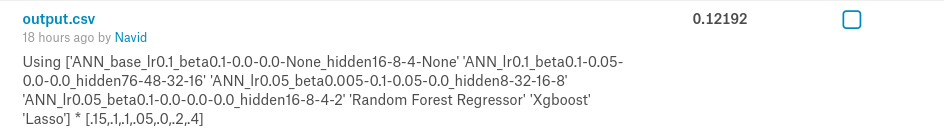
\includegraphics{img/kaggle_score.png}
\end{itemize}

\subsubsection{Best score without Ensemble : 0.12324 (ANN
only)}\label{best-score-without-ensemble-0.12324-ann-only}

\begin{itemize}
\tightlist
\item
  
\includegraphics{img/ann_base.png}
\end{itemize}

    \section{Imports:}\label{imports}

In the following section, I have imported all the necessary libraries
that I will need to properly complete the assignment. - The 'Pandas'
library will be used to store the 'Train' and 'Test' datasets. The
particular data storing format is called a 'Dataframe'. - The 'Numpy'
library is used to make mathematical calculations easier and faster to
do. - 'Matplotlib' and 'Seaborn' are used to plot graphs - From the
'Scikit learn'(sklearn) library, I have imported some data processing
methods, some evaluation metrics and some predictive models.

    \paragraph{Gpu testing}\label{gpu-testing}

    \begin{Verbatim}[commandchars=\\\{\}]
{\color{incolor}In [{\color{incolor}73}]:} \PY{k+kn}{import} \PY{n+nn}{tensorflow} \PY{k}{as} \PY{n+nn}{tf}
         \PY{n}{device\PYZus{}name} \PY{o}{=} \PY{n}{tf}\PY{o}{.}\PY{n}{test}\PY{o}{.}\PY{n}{gpu\PYZus{}device\PYZus{}name}\PY{p}{(}\PY{p}{)}
         \PY{k}{if} \PY{n}{device\PYZus{}name} \PY{o}{!=} \PY{l+s+s1}{\PYZsq{}}\PY{l+s+s1}{/device:GPU:0}\PY{l+s+s1}{\PYZsq{}}\PY{p}{:}
           \PY{k}{raise} \PY{n+ne}{SystemError}\PY{p}{(}\PY{l+s+s1}{\PYZsq{}}\PY{l+s+s1}{GPU device not found}\PY{l+s+s1}{\PYZsq{}}\PY{p}{)}
         \PY{n+nb}{print}\PY{p}{(}\PY{l+s+s1}{\PYZsq{}}\PY{l+s+s1}{Found GPU at: }\PY{l+s+si}{\PYZob{}\PYZcb{}}\PY{l+s+s1}{\PYZsq{}}\PY{o}{.}\PY{n}{format}\PY{p}{(}\PY{n}{device\PYZus{}name}\PY{p}{)}\PY{p}{)}
\end{Verbatim}

    \begin{Verbatim}[commandchars=\\\{\}]
Found GPU at: /device:GPU:0

    \end{Verbatim}

    \begin{Verbatim}[commandchars=\\\{\}]
{\color{incolor}In [{\color{incolor}74}]:} \PY{k+kn}{import} \PY{n+nn}{tensorflow} \PY{k}{as} \PY{n+nn}{tf}
         \PY{k+kn}{import} \PY{n+nn}{numpy} \PY{k}{as} \PY{n+nn}{np}
         \PY{k+kn}{import} \PY{n+nn}{pandas} \PY{k}{as} \PY{n+nn}{pd}
         \PY{k+kn}{from} \PY{n+nn}{sklearn}\PY{n+nn}{.}\PY{n+nn}{ensemble} \PY{k}{import} \PY{n}{RandomForestRegressor}
         \PY{k+kn}{from} \PY{n+nn}{sklearn}\PY{n+nn}{.}\PY{n+nn}{impute} \PY{k}{import} \PY{n}{SimpleImputer}
         \PY{k+kn}{from} \PY{n+nn}{sklearn}\PY{n+nn}{.}\PY{n+nn}{model\PYZus{}selection} \PY{k}{import} \PY{n}{train\PYZus{}test\PYZus{}split}
         \PY{k+kn}{from} \PY{n+nn}{sklearn}\PY{n+nn}{.}\PY{n+nn}{metrics} \PY{k}{import} \PY{n}{mean\PYZus{}squared\PYZus{}error}
         \PY{k+kn}{from} \PY{n+nn}{sklearn}\PY{n+nn}{.}\PY{n+nn}{metrics} \PY{k}{import}  \PY{n}{r2\PYZus{}score}
         \PY{k+kn}{from} \PY{n+nn}{sklearn}\PY{n+nn}{.}\PY{n+nn}{linear\PYZus{}model} \PY{k}{import} \PY{n}{LinearRegression}
         \PY{k+kn}{from} \PY{n+nn}{sklearn}\PY{n+nn}{.}\PY{n+nn}{preprocessing} \PY{k}{import} \PY{n}{OneHotEncoder}
         \PY{k+kn}{from} \PY{n+nn}{sklearn}\PY{n+nn}{.}\PY{n+nn}{preprocessing} \PY{k}{import} \PY{n}{StandardScaler}
         \PY{k+kn}{from} \PY{n+nn}{IPython}\PY{n+nn}{.}\PY{n+nn}{display} \PY{k}{import} \PY{n}{Image}
         \PY{k+kn}{from} \PY{n+nn}{sklearn}\PY{n+nn}{.}\PY{n+nn}{preprocessing} \PY{k}{import} \PY{n}{normalize}\PY{p}{,}\PY{n}{MinMaxScaler}
         \PY{k+kn}{import} \PY{n+nn}{matplotlib}\PY{n+nn}{.}\PY{n+nn}{pyplot} \PY{k}{as} \PY{n+nn}{plt}
         \PY{k+kn}{from} \PY{n+nn}{sklearn}\PY{n+nn}{.}\PY{n+nn}{utils} \PY{k}{import} \PY{n}{shuffle}
         \PY{k+kn}{import} \PY{n+nn}{seaborn} \PY{k}{as} \PY{n+nn}{sns}
         \PY{c+c1}{\PYZsh{} \PYZpc{}matplotlib widget}
         \PY{o}{\PYZpc{}}\PY{k}{matplotlib} inline
\end{Verbatim}

    \section{Data Pre-processing}\label{data-pre-processing}

    \subsubsection{Load Data}\label{load-data}

The following block of code reads the two CSV (Comma Separated Values)
files and then stores the data inside them in two separate Dataframes
named 'train' and 'test'.

    \begin{Verbatim}[commandchars=\\\{\}]
{\color{incolor}In [{\color{incolor}75}]:} \PY{n}{train} \PY{o}{=} \PY{n}{pd}\PY{o}{.}\PY{n}{read\PYZus{}csv}\PY{p}{(}\PY{l+s+s1}{\PYZsq{}}\PY{l+s+s1}{train.csv}\PY{l+s+s1}{\PYZsq{}}\PY{p}{)}\PY{c+c1}{\PYZsh{}.select\PYZus{}dtypes(exclude=[\PYZsq{}object\PYZsq{}])}
         \PY{n}{test} \PY{o}{=} \PY{n}{pd}\PY{o}{.}\PY{n}{read\PYZus{}csv}\PY{p}{(}\PY{l+s+s1}{\PYZsq{}}\PY{l+s+s1}{test.csv}\PY{l+s+s1}{\PYZsq{}}\PY{p}{)}\PY{c+c1}{\PYZsh{}.select\PYZus{}dtypes(exclude=[\PYZsq{}object\PYZsq{}])}
         
         \PY{c+c1}{\PYZsh{}look into datatypes of the file}
         \PY{n+nb}{print}\PY{p}{(}\PY{l+s+s2}{\PYZdq{}}\PY{l+s+s2}{data types count}\PY{l+s+s2}{\PYZdq{}}\PY{p}{)}
         \PY{n}{train}\PY{o}{.}\PY{n}{dtypes}\PY{o}{.}\PY{n}{groupby}\PY{p}{(}\PY{n}{train}\PY{o}{.}\PY{n}{dtypes}\PY{p}{)}\PY{o}{.}\PY{n}{count}\PY{p}{(}\PY{p}{)}
\end{Verbatim}

    \begin{Verbatim}[commandchars=\\\{\}]
data types count

    \end{Verbatim}

\begin{Verbatim}[commandchars=\\\{\}]
{\color{outcolor}Out[{\color{outcolor}75}]:} int64      35
         float64     3
         object     43
         dtype: int64
\end{Verbatim}
            
    \subsubsection{Looking into data}\label{looking-into-data}

    Here I am printing the first five entries in the train dataset to look
into the actual data that I will be working with. I gives me some
insight about the data I am working with.

    \begin{Verbatim}[commandchars=\\\{\}]
{\color{incolor}In [{\color{incolor}76}]:} \PY{n+nb}{print}\PY{p}{(}\PY{l+s+s1}{\PYZsq{}}\PY{l+s+s1}{show sample}\PY{l+s+s1}{\PYZsq{}}\PY{p}{)}
         \PY{n}{pd}\PY{o}{.}\PY{n}{set\PYZus{}option}\PY{p}{(}\PY{l+s+s1}{\PYZsq{}}\PY{l+s+s1}{display.max\PYZus{}column}\PY{l+s+s1}{\PYZsq{}}\PY{p}{,} \PY{k+kc}{None}\PY{p}{)}
         \PY{n}{train}\PY{o}{.}\PY{n}{head}\PY{p}{(}\PY{p}{)}
\end{Verbatim}

    \begin{Verbatim}[commandchars=\\\{\}]
show sample

    \end{Verbatim}

\begin{Verbatim}[commandchars=\\\{\}]
{\color{outcolor}Out[{\color{outcolor}76}]:}    Id  MSSubClass MSZoning  LotFrontage  LotArea Street Alley LotShape  \textbackslash{}
         0   1          60       RL         65.0     8450   Pave   NaN      Reg   
         1   2          20       RL         80.0     9600   Pave   NaN      Reg   
         2   3          60       RL         68.0    11250   Pave   NaN      IR1   
         3   4          70       RL         60.0     9550   Pave   NaN      IR1   
         4   5          60       RL         84.0    14260   Pave   NaN      IR1   
         
           LandContour Utilities LotConfig LandSlope Neighborhood Condition1  \textbackslash{}
         0         Lvl    AllPub    Inside       Gtl      CollgCr       Norm   
         1         Lvl    AllPub       FR2       Gtl      Veenker      Feedr   
         2         Lvl    AllPub    Inside       Gtl      CollgCr       Norm   
         3         Lvl    AllPub    Corner       Gtl      Crawfor       Norm   
         4         Lvl    AllPub       FR2       Gtl      NoRidge       Norm   
         
           Condition2 BldgType HouseStyle  OverallQual  OverallCond  YearBuilt  \textbackslash{}
         0       Norm     1Fam     2Story            7            5       2003   
         1       Norm     1Fam     1Story            6            8       1976   
         2       Norm     1Fam     2Story            7            5       2001   
         3       Norm     1Fam     2Story            7            5       1915   
         4       Norm     1Fam     2Story            8            5       2000   
         
            YearRemodAdd RoofStyle RoofMatl Exterior1st Exterior2nd MasVnrType  \textbackslash{}
         0          2003     Gable  CompShg     VinylSd     VinylSd    BrkFace   
         1          1976     Gable  CompShg     MetalSd     MetalSd       None   
         2          2002     Gable  CompShg     VinylSd     VinylSd    BrkFace   
         3          1970     Gable  CompShg     Wd Sdng     Wd Shng       None   
         4          2000     Gable  CompShg     VinylSd     VinylSd    BrkFace   
         
            MasVnrArea ExterQual ExterCond Foundation BsmtQual BsmtCond BsmtExposure  \textbackslash{}
         0       196.0        Gd        TA      PConc       Gd       TA           No   
         1         0.0        TA        TA     CBlock       Gd       TA           Gd   
         2       162.0        Gd        TA      PConc       Gd       TA           Mn   
         3         0.0        TA        TA     BrkTil       TA       Gd           No   
         4       350.0        Gd        TA      PConc       Gd       TA           Av   
         
           BsmtFinType1  BsmtFinSF1 BsmtFinType2  BsmtFinSF2  BsmtUnfSF  TotalBsmtSF  \textbackslash{}
         0          GLQ         706          Unf           0        150          856   
         1          ALQ         978          Unf           0        284         1262   
         2          GLQ         486          Unf           0        434          920   
         3          ALQ         216          Unf           0        540          756   
         4          GLQ         655          Unf           0        490         1145   
         
           Heating HeatingQC CentralAir Electrical  1stFlrSF  2ndFlrSF  LowQualFinSF  \textbackslash{}
         0    GasA        Ex          Y      SBrkr       856       854             0   
         1    GasA        Ex          Y      SBrkr      1262         0             0   
         2    GasA        Ex          Y      SBrkr       920       866             0   
         3    GasA        Gd          Y      SBrkr       961       756             0   
         4    GasA        Ex          Y      SBrkr      1145      1053             0   
         
            GrLivArea  BsmtFullBath  BsmtHalfBath  FullBath  HalfBath  BedroomAbvGr  \textbackslash{}
         0       1710             1             0         2         1             3   
         1       1262             0             1         2         0             3   
         2       1786             1             0         2         1             3   
         3       1717             1             0         1         0             3   
         4       2198             1             0         2         1             4   
         
            KitchenAbvGr KitchenQual  TotRmsAbvGrd Functional  Fireplaces FireplaceQu  \textbackslash{}
         0             1          Gd             8        Typ           0         NaN   
         1             1          TA             6        Typ           1          TA   
         2             1          Gd             6        Typ           1          TA   
         3             1          Gd             7        Typ           1          Gd   
         4             1          Gd             9        Typ           1          TA   
         
           GarageType  GarageYrBlt GarageFinish  GarageCars  GarageArea GarageQual  \textbackslash{}
         0     Attchd       2003.0          RFn           2         548         TA   
         1     Attchd       1976.0          RFn           2         460         TA   
         2     Attchd       2001.0          RFn           2         608         TA   
         3     Detchd       1998.0          Unf           3         642         TA   
         4     Attchd       2000.0          RFn           3         836         TA   
         
           GarageCond PavedDrive  WoodDeckSF  OpenPorchSF  EnclosedPorch  3SsnPorch  \textbackslash{}
         0         TA          Y           0           61              0          0   
         1         TA          Y         298            0              0          0   
         2         TA          Y           0           42              0          0   
         3         TA          Y           0           35            272          0   
         4         TA          Y         192           84              0          0   
         
            ScreenPorch  PoolArea PoolQC Fence MiscFeature  MiscVal  MoSold  YrSold  \textbackslash{}
         0            0         0    NaN   NaN         NaN        0       2    2008   
         1            0         0    NaN   NaN         NaN        0       5    2007   
         2            0         0    NaN   NaN         NaN        0       9    2008   
         3            0         0    NaN   NaN         NaN        0       2    2006   
         4            0         0    NaN   NaN         NaN        0      12    2008   
         
           SaleType SaleCondition  SalePrice  
         0       WD        Normal     208500  
         1       WD        Normal     181500  
         2       WD        Normal     223500  
         3       WD       Abnorml     140000  
         4       WD        Normal     250000  
\end{Verbatim}
            
    Here I have used one of the built-in functions of pandas dataframe to
display descriptive statistics that summarize the central tendency,
dispersion and shape of a dataset's distribution, excluding NaN values.

    \begin{Verbatim}[commandchars=\\\{\}]
{\color{incolor}In [{\color{incolor}77}]:} \PY{n+nb}{print}\PY{p}{(}\PY{l+s+s1}{\PYZsq{}}\PY{l+s+s1}{description of data}\PY{l+s+s1}{\PYZsq{}}\PY{p}{)}
         \PY{n}{train}\PY{o}{.}\PY{n}{describe}\PY{p}{(}\PY{p}{)}
\end{Verbatim}

    \begin{Verbatim}[commandchars=\\\{\}]
description of data

    \end{Verbatim}

\begin{Verbatim}[commandchars=\\\{\}]
{\color{outcolor}Out[{\color{outcolor}77}]:}                 Id   MSSubClass  LotFrontage        LotArea  OverallQual  \textbackslash{}
         count  1460.000000  1460.000000  1201.000000    1460.000000  1460.000000   
         mean    730.500000    56.897260    70.049958   10516.828082     6.099315   
         std     421.610009    42.300571    24.284752    9981.264932     1.382997   
         min       1.000000    20.000000    21.000000    1300.000000     1.000000   
         25\%     365.750000    20.000000    59.000000    7553.500000     5.000000   
         50\%     730.500000    50.000000    69.000000    9478.500000     6.000000   
         75\%    1095.250000    70.000000    80.000000   11601.500000     7.000000   
         max    1460.000000   190.000000   313.000000  215245.000000    10.000000   
         
                OverallCond    YearBuilt  YearRemodAdd   MasVnrArea   BsmtFinSF1  \textbackslash{}
         count  1460.000000  1460.000000   1460.000000  1452.000000  1460.000000   
         mean      5.575342  1971.267808   1984.865753   103.685262   443.639726   
         std       1.112799    30.202904     20.645407   181.066207   456.098091   
         min       1.000000  1872.000000   1950.000000     0.000000     0.000000   
         25\%       5.000000  1954.000000   1967.000000     0.000000     0.000000   
         50\%       5.000000  1973.000000   1994.000000     0.000000   383.500000   
         75\%       6.000000  2000.000000   2004.000000   166.000000   712.250000   
         max       9.000000  2010.000000   2010.000000  1600.000000  5644.000000   
         
                 BsmtFinSF2    BsmtUnfSF  TotalBsmtSF     1stFlrSF     2ndFlrSF  \textbackslash{}
         count  1460.000000  1460.000000  1460.000000  1460.000000  1460.000000   
         mean     46.549315   567.240411  1057.429452  1162.626712   346.992466   
         std     161.319273   441.866955   438.705324   386.587738   436.528436   
         min       0.000000     0.000000     0.000000   334.000000     0.000000   
         25\%       0.000000   223.000000   795.750000   882.000000     0.000000   
         50\%       0.000000   477.500000   991.500000  1087.000000     0.000000   
         75\%       0.000000   808.000000  1298.250000  1391.250000   728.000000   
         max    1474.000000  2336.000000  6110.000000  4692.000000  2065.000000   
         
                LowQualFinSF    GrLivArea  BsmtFullBath  BsmtHalfBath     FullBath  \textbackslash{}
         count   1460.000000  1460.000000   1460.000000   1460.000000  1460.000000   
         mean       5.844521  1515.463699      0.425342      0.057534     1.565068   
         std       48.623081   525.480383      0.518911      0.238753     0.550916   
         min        0.000000   334.000000      0.000000      0.000000     0.000000   
         25\%        0.000000  1129.500000      0.000000      0.000000     1.000000   
         50\%        0.000000  1464.000000      0.000000      0.000000     2.000000   
         75\%        0.000000  1776.750000      1.000000      0.000000     2.000000   
         max      572.000000  5642.000000      3.000000      2.000000     3.000000   
         
                   HalfBath  BedroomAbvGr  KitchenAbvGr  TotRmsAbvGrd   Fireplaces  \textbackslash{}
         count  1460.000000   1460.000000   1460.000000   1460.000000  1460.000000   
         mean      0.382877      2.866438      1.046575      6.517808     0.613014   
         std       0.502885      0.815778      0.220338      1.625393     0.644666   
         min       0.000000      0.000000      0.000000      2.000000     0.000000   
         25\%       0.000000      2.000000      1.000000      5.000000     0.000000   
         50\%       0.000000      3.000000      1.000000      6.000000     1.000000   
         75\%       1.000000      3.000000      1.000000      7.000000     1.000000   
         max       2.000000      8.000000      3.000000     14.000000     3.000000   
         
                GarageYrBlt   GarageCars   GarageArea   WoodDeckSF  OpenPorchSF  \textbackslash{}
         count  1379.000000  1460.000000  1460.000000  1460.000000  1460.000000   
         mean   1978.506164     1.767123   472.980137    94.244521    46.660274   
         std      24.689725     0.747315   213.804841   125.338794    66.256028   
         min    1900.000000     0.000000     0.000000     0.000000     0.000000   
         25\%    1961.000000     1.000000   334.500000     0.000000     0.000000   
         50\%    1980.000000     2.000000   480.000000     0.000000    25.000000   
         75\%    2002.000000     2.000000   576.000000   168.000000    68.000000   
         max    2010.000000     4.000000  1418.000000   857.000000   547.000000   
         
                EnclosedPorch    3SsnPorch  ScreenPorch     PoolArea       MiscVal  \textbackslash{}
         count    1460.000000  1460.000000  1460.000000  1460.000000   1460.000000   
         mean       21.954110     3.409589    15.060959     2.758904     43.489041   
         std        61.119149    29.317331    55.757415    40.177307    496.123024   
         min         0.000000     0.000000     0.000000     0.000000      0.000000   
         25\%         0.000000     0.000000     0.000000     0.000000      0.000000   
         50\%         0.000000     0.000000     0.000000     0.000000      0.000000   
         75\%         0.000000     0.000000     0.000000     0.000000      0.000000   
         max       552.000000   508.000000   480.000000   738.000000  15500.000000   
         
                     MoSold       YrSold      SalePrice  
         count  1460.000000  1460.000000    1460.000000  
         mean      6.321918  2007.815753  180921.195890  
         std       2.703626     1.328095   79442.502883  
         min       1.000000  2006.000000   34900.000000  
         25\%       5.000000  2007.000000  129975.000000  
         50\%       6.000000  2008.000000  163000.000000  
         75\%       8.000000  2009.000000  214000.000000  
         max      12.000000  2010.000000  755000.000000  
\end{Verbatim}
            
    This function shows scatter-plot and distribution plot. I am going to
use it to see few of the features of the dataset and observe how it
changes while I process the data. I will try not to remove data so
instead of removing any data point I will observe them until all my data
processing is complete. If I found out after all the processing some
data points are really causing problem then I will drop it.

    \begin{Verbatim}[commandchars=\\\{\}]
{\color{incolor}In [{\color{incolor}78}]:} \PY{c+c1}{\PYZsh{}For showing diffrence }
         \PY{n}{old\PYZus{}train\PYZus{}outlier\PYZus{}flag} \PY{o}{=}\PY{n}{train}\PY{o}{.}\PY{n}{copy}\PY{p}{(}\PY{p}{)}
         \PY{n}{old\PYZus{}test\PYZus{}outlier\PYZus{}flag} \PY{o}{=}\PY{n}{test}\PY{o}{.}\PY{n}{copy}\PY{p}{(}\PY{p}{)}
         \PY{n}{old\PYZus{}target\PYZus{}outlier\PYZus{}flag} \PY{o}{=}\PY{n}{train}\PY{o}{.}\PY{n}{SalePrice}\PY{o}{.}\PY{n}{copy}\PY{p}{(}\PY{p}{)}
         
         \PY{c+c1}{\PYZsh{} A FUNCTION THAT SHOWS SCATTER\PYZhy{}PLOT AND DISTRIBUTION\PYZhy{}PLOT}
         \PY{k}{def} \PY{n+nf}{outlier\PYZus{}check\PYZus{}plot}\PY{p}{(}\PY{n}{column}\PY{p}{,} \PY{n}{train\PYZus{}data\PYZus{}flag}\PY{o}{=}\PY{n}{train} \PY{p}{,} \PY{n}{test\PYZus{}data\PYZus{}flag}\PY{o}{=}\PY{n}{test} \PY{p}{,} \PY{n}{target}\PY{o}{=}\PY{n}{train}\PY{o}{.}\PY{n}{SalePrice} \PY{p}{)}\PY{p}{:}
             \PY{n}{plt}\PY{o}{.}\PY{n}{subplots}\PY{p}{(}\PY{n}{figsize}\PY{o}{=}\PY{p}{(}\PY{l+m+mi}{19}\PY{p}{,} \PY{l+m+mi}{5}\PY{p}{)}\PY{p}{)}
             \PY{c+c1}{\PYZsh{} SCATTER PLOT OF THE 19 HIGHEST\PYZhy{}VALUES OF A COLUMN}
             \PY{n}{plt}\PY{o}{.}\PY{n}{subplot}\PY{p}{(}\PY{l+m+mi}{1}\PY{p}{,} \PY{l+m+mi}{3}\PY{p}{,} \PY{l+m+mi}{1}\PY{p}{)}
             \PY{n}{plt}\PY{o}{.}\PY{n}{scatter}\PY{p}{(}\PY{n}{x} \PY{o}{=} \PY{n}{train\PYZus{}data\PYZus{}flag}\PY{p}{[}\PY{n}{column}\PY{p}{]}\PY{o}{.}\PY{n}{sort\PYZus{}values}\PY{p}{(}\PY{n}{ascending}\PY{o}{=}\PY{k+kc}{False}\PY{p}{)}\PY{p}{[}\PY{p}{:}\PY{l+m+mi}{19}\PY{p}{]}\PY{p}{,} \PY{n}{y} \PY{o}{=} \PY{n}{train}\PY{o}{.}\PY{n}{Id}\PY{p}{[}\PY{p}{:}\PY{l+m+mi}{19}\PY{p}{]}\PY{p}{,} \PY{n}{color}\PY{o}{=}\PY{l+s+s1}{\PYZsq{}}\PY{l+s+s1}{red}\PY{l+s+s1}{\PYZsq{}}\PY{p}{,} \PY{n}{label}\PY{o}{=}\PY{l+s+s1}{\PYZsq{}}\PY{l+s+s1}{Train}\PY{l+s+s1}{\PYZsq{}} \PY{p}{)}
             \PY{n}{plt}\PY{o}{.}\PY{n}{scatter}\PY{p}{(}\PY{n}{x} \PY{o}{=} \PY{n}{test\PYZus{}data\PYZus{}flag}\PY{p}{[}\PY{n}{column}\PY{p}{]}\PY{o}{.}\PY{n}{sort\PYZus{}values}\PY{p}{(}\PY{n}{ascending}\PY{o}{=}\PY{k+kc}{False}\PY{p}{)}\PY{p}{[}\PY{p}{:}\PY{l+m+mi}{19}\PY{p}{]}\PY{p}{,} \PY{n}{y} \PY{o}{=} \PY{n}{test}\PY{o}{.}\PY{n}{Id}\PY{p}{[}\PY{p}{:}\PY{l+m+mi}{19}\PY{p}{]}\PY{p}{,} \PY{n}{label}\PY{o}{=}\PY{l+s+s1}{\PYZsq{}}\PY{l+s+s1}{Test}\PY{l+s+s1}{\PYZsq{}}\PY{p}{)}
             \PY{n}{plt}\PY{o}{.}\PY{n}{ylabel}\PY{p}{(}\PY{l+s+s1}{\PYZsq{}}\PY{l+s+s1}{Serial Number}\PY{l+s+s1}{\PYZsq{}}\PY{p}{,} \PY{n}{fontsize}\PY{o}{=}\PY{l+m+mi}{13}\PY{p}{)}
             \PY{n}{plt}\PY{o}{.}\PY{n}{xlabel}\PY{p}{(}\PY{n}{column}\PY{p}{,} \PY{n}{fontsize}\PY{o}{=}\PY{l+m+mi}{13}\PY{p}{)}
             \PY{n}{plt}\PY{o}{.}\PY{n}{title}\PY{p}{(}\PY{l+s+s1}{\PYZsq{}}\PY{l+s+s1}{Fig 1: 19 highest\PYZhy{}values of category }\PY{l+s+si}{\PYZob{}\PYZcb{}}\PY{l+s+s1}{ }\PY{l+s+se}{\PYZbs{}n}\PY{l+s+s1}{ in both train and test dataset}\PY{l+s+s1}{\PYZsq{}}\PY{o}{.}\PY{n}{format}\PY{p}{(}\PY{n}{column}\PY{p}{)}\PY{p}{)}
             \PY{n}{plt}\PY{o}{.}\PY{n}{legend}\PY{p}{(}\PY{n}{loc}\PY{o}{=}\PY{l+s+s1}{\PYZsq{}}\PY{l+s+s1}{center}\PY{l+s+s1}{\PYZsq{}}\PY{p}{,}\PY{n}{fontsize}\PY{o}{=}\PY{l+m+mi}{13}\PY{p}{)}
             \PY{c+c1}{\PYZsh{} DISTRIBUTION\PYZhy{}PLOT OF THE COLUMN}
             \PY{n}{plt}\PY{o}{.}\PY{n}{subplot}\PY{p}{(}\PY{l+m+mi}{1}\PY{p}{,} \PY{l+m+mi}{3}\PY{p}{,} \PY{l+m+mi}{2}\PY{p}{)}
             \PY{n}{sns}\PY{o}{.}\PY{n}{distplot}\PY{p}{(}\PY{n}{train\PYZus{}data\PYZus{}flag}\PY{p}{[}\PY{n}{column}\PY{p}{]}\PY{p}{,}\PY{n}{color}\PY{o}{=}\PY{l+s+s1}{\PYZsq{}}\PY{l+s+s1}{red}\PY{l+s+s1}{\PYZsq{}}\PY{p}{,} \PY{n}{rug}\PY{o}{=}\PY{k+kc}{True}\PY{p}{,} \PY{n}{hist}\PY{o}{=}\PY{k+kc}{False}\PY{p}{,} \PY{n}{label}\PY{o}{=}\PY{l+s+s1}{\PYZsq{}}\PY{l+s+s1}{Train}\PY{l+s+s1}{\PYZsq{}}\PY{p}{)}
             \PY{n}{sns}\PY{o}{.}\PY{n}{distplot}\PY{p}{(}\PY{n}{test\PYZus{}data\PYZus{}flag}\PY{p}{[}\PY{n}{column}\PY{p}{]}\PY{p}{,} \PY{n}{rug}\PY{o}{=}\PY{k+kc}{True}\PY{p}{,} \PY{n}{hist}\PY{o}{=}\PY{k+kc}{False}\PY{p}{,} \PY{n}{label}\PY{o}{=}\PY{l+s+s1}{\PYZsq{}}\PY{l+s+s1}{Test}\PY{l+s+s1}{\PYZsq{}}\PY{p}{)}
             \PY{n}{plt}\PY{o}{.}\PY{n}{ylabel}\PY{p}{(}\PY{l+s+s1}{\PYZsq{}}\PY{l+s+s1}{Distribution}\PY{l+s+s1}{\PYZsq{}}\PY{p}{,} \PY{n}{fontsize}\PY{o}{=}\PY{l+m+mi}{13}\PY{p}{)}
             \PY{n}{plt}\PY{o}{.}\PY{n}{xlabel}\PY{p}{(}\PY{n}{column}\PY{p}{,} \PY{n}{fontsize}\PY{o}{=}\PY{l+m+mi}{13}\PY{p}{)}
             \PY{n}{plt}\PY{o}{.}\PY{n}{title}\PY{p}{(}\PY{l+s+s1}{\PYZsq{}}\PY{l+s+s1}{Fig 2: Distribution\PYZhy{}plot of category }\PY{l+s+si}{\PYZob{}\PYZcb{}}\PY{l+s+s1}{ }\PY{l+s+se}{\PYZbs{}n}\PY{l+s+s1}{ for both train and test dataset}\PY{l+s+s1}{\PYZsq{}}\PY{o}{.}\PY{n}{format}\PY{p}{(}\PY{n}{column}\PY{p}{)}\PY{p}{)}
             \PY{n}{plt}\PY{o}{.}\PY{n}{legend}\PY{p}{(}\PY{n}{fontsize}\PY{o}{=}\PY{l+m+mi}{13}\PY{p}{)}
             \PY{c+c1}{\PYZsh{} SCATTER\PYZhy{}PLOT OF THE COLUMN WITH RESPECT TO SALEPRICE}
             \PY{n}{plt}\PY{o}{.}\PY{n}{subplot}\PY{p}{(}\PY{l+m+mi}{1}\PY{p}{,} \PY{l+m+mi}{3}\PY{p}{,} \PY{l+m+mi}{3}\PY{p}{)}
             \PY{n}{plt}\PY{o}{.}\PY{n}{scatter}\PY{p}{(}\PY{n}{x} \PY{o}{=} \PY{n}{train\PYZus{}data\PYZus{}flag}\PY{p}{[}\PY{n}{column}\PY{p}{]}\PY{p}{,} \PY{n}{y} \PY{o}{=} \PY{n}{target}\PY{p}{)}
             \PY{n}{plt}\PY{o}{.}\PY{n}{ylabel}\PY{p}{(}\PY{l+s+s1}{\PYZsq{}}\PY{l+s+s1}{SalePrice}\PY{l+s+s1}{\PYZsq{}}\PY{p}{,} \PY{n}{fontsize}\PY{o}{=}\PY{l+m+mi}{13}\PY{p}{)}
             \PY{n}{plt}\PY{o}{.}\PY{n}{xlabel}\PY{p}{(}\PY{n}{column}\PY{p}{,} \PY{n}{fontsize}\PY{o}{=}\PY{l+m+mi}{13}\PY{p}{)}
             \PY{n}{plt}\PY{o}{.}\PY{n}{title}\PY{p}{(}\PY{l+s+s1}{\PYZsq{}}\PY{l+s+s1}{Fig 3: Scatter\PYZhy{}plot of train\PYZhy{}category }\PY{l+s+si}{\PYZob{}\PYZcb{}}\PY{l+s+s1}{ }\PY{l+s+se}{\PYZbs{}n}\PY{l+s+s1}{ with respect to SalePrice}\PY{l+s+s1}{\PYZsq{}}\PY{o}{.}\PY{n}{format}\PY{p}{(}\PY{n}{column}\PY{p}{)}\PY{p}{)}
             \PY{n}{plt}\PY{o}{.}\PY{n}{show}\PY{p}{(}\PY{p}{)}
\end{Verbatim}

    \begin{Verbatim}[commandchars=\\\{\}]
{\color{incolor}In [{\color{incolor}79}]:} \PY{n+nb}{print}\PY{p}{(}\PY{l+s+s1}{\PYZsq{}}\PY{l+s+s1}{Before outlier\PYZhy{}removal of 1stFlrSF: }\PY{l+s+s1}{\PYZsq{}}\PY{p}{)}
         \PY{n}{outlier\PYZus{}check\PYZus{}plot}\PY{p}{(}\PY{l+s+s1}{\PYZsq{}}\PY{l+s+s1}{1stFlrSF}\PY{l+s+s1}{\PYZsq{}}\PY{p}{)}
\end{Verbatim}

    \begin{Verbatim}[commandchars=\\\{\}]
Before outlier-removal of 1stFlrSF: 

    \end{Verbatim}

    \begin{center}
    \adjustimage{max size={0.9\linewidth}{0.9\paperheight}}{output_19_1.png}
    \end{center}
    { \hspace*{\fill} \\}
    
    We can see one value in train set that is highly contradictory with
SalePrice (1stFlrSF is too high but SalePrice is too low). And there is
only one such high-value point available in test dataset. So we might
want to remove this outlier.

    \begin{Verbatim}[commandchars=\\\{\}]
{\color{incolor}In [{\color{incolor}80}]:} \PY{n+nb}{print}\PY{p}{(}\PY{l+s+s1}{\PYZsq{}}\PY{l+s+s1}{Before outlier\PYZhy{}removal of BsmtFinSF1: }\PY{l+s+s1}{\PYZsq{}}\PY{p}{)}
         \PY{n}{outlier\PYZus{}check\PYZus{}plot}\PY{p}{(}\PY{l+s+s1}{\PYZsq{}}\PY{l+s+s1}{BsmtFinSF1}\PY{l+s+s1}{\PYZsq{}}\PY{p}{)}
\end{Verbatim}

    \begin{Verbatim}[commandchars=\\\{\}]
Before outlier-removal of BsmtFinSF1: 

    \end{Verbatim}

    \begin{Verbatim}[commandchars=\\\{\}]
/home/navid/anaconda3/envs/tf/lib/python3.6/site-packages/statsmodels/nonparametric/kde.py:448: RuntimeWarning: invalid value encountered in greater
  X = X[np.logical\_and(X > clip[0], X < clip[1])] \# won't work for two columns.
/home/navid/anaconda3/envs/tf/lib/python3.6/site-packages/statsmodels/nonparametric/kde.py:448: RuntimeWarning: invalid value encountered in less
  X = X[np.logical\_and(X > clip[0], X < clip[1])] \# won't work for two columns.

    \end{Verbatim}

    \begin{center}
    \adjustimage{max size={0.9\linewidth}{0.9\paperheight}}{output_21_2.png}
    \end{center}
    { \hspace*{\fill} \\}
    
    We can also see the same outlier here.

    \begin{Verbatim}[commandchars=\\\{\}]
{\color{incolor}In [{\color{incolor}81}]:} \PY{n+nb}{print}\PY{p}{(}\PY{l+s+s1}{\PYZsq{}}\PY{l+s+s1}{Before outlier\PYZhy{}removal of LotArea: }\PY{l+s+s1}{\PYZsq{}}\PY{p}{)}
         \PY{n}{outlier\PYZus{}check\PYZus{}plot}\PY{p}{(}\PY{l+s+s1}{\PYZsq{}}\PY{l+s+s1}{LotArea}\PY{l+s+s1}{\PYZsq{}}\PY{p}{)}
\end{Verbatim}

    \begin{Verbatim}[commandchars=\\\{\}]
Before outlier-removal of LotArea: 

    \end{Verbatim}

    \begin{center}
    \adjustimage{max size={0.9\linewidth}{0.9\paperheight}}{output_23_1.png}
    \end{center}
    { \hspace*{\fill} \\}
    
    We can see in Fig 3 that there are 4 LotArea train-samples above 80000
that are very high in size but comperatively very low in SalePrice. Also
there are no such values present in test-data: Fig 1. So we can drop
them

    \begin{Verbatim}[commandchars=\\\{\}]
{\color{incolor}In [{\color{incolor}82}]:} \PY{n+nb}{print}\PY{p}{(}\PY{l+s+s1}{\PYZsq{}}\PY{l+s+s1}{Before outlier\PYZhy{}removal of GrLivArea: }\PY{l+s+s1}{\PYZsq{}}\PY{p}{)}
         \PY{n}{outlier\PYZus{}check\PYZus{}plot}\PY{p}{(}\PY{l+s+s1}{\PYZsq{}}\PY{l+s+s1}{GrLivArea}\PY{l+s+s1}{\PYZsq{}}\PY{p}{)}
\end{Verbatim}

    \begin{Verbatim}[commandchars=\\\{\}]
Before outlier-removal of GrLivArea: 

    \end{Verbatim}

    \begin{center}
    \adjustimage{max size={0.9\linewidth}{0.9\paperheight}}{output_25_1.png}
    \end{center}
    { \hspace*{\fill} \\}
    
    If we compare Fig. 3 with code-cell 13 we can see that two outliers are
already common in GrLivArea. These two outliers of GrLivArea
train-samples were above 4000 with very low SalePrice (below 300000). We
are seeing same outlier again and again.

    \begin{Verbatim}[commandchars=\\\{\}]
{\color{incolor}In [{\color{incolor}83}]:} \PY{n+nb}{print}\PY{p}{(}\PY{l+s+s1}{\PYZsq{}}\PY{l+s+s1}{Before outlier\PYZhy{}removal of MasVnrArea: }\PY{l+s+s1}{\PYZsq{}}\PY{p}{)}
         \PY{n}{outlier\PYZus{}check\PYZus{}plot}\PY{p}{(}\PY{l+s+s1}{\PYZsq{}}\PY{l+s+s1}{MasVnrArea}\PY{l+s+s1}{\PYZsq{}}\PY{p}{)}
\end{Verbatim}

    \begin{Verbatim}[commandchars=\\\{\}]
Before outlier-removal of MasVnrArea: 

    \end{Verbatim}

    \begin{center}
    \adjustimage{max size={0.9\linewidth}{0.9\paperheight}}{output_27_1.png}
    \end{center}
    { \hspace*{\fill} \\}
    
    As we can see in Fig 3 that above 1500 there is 1 MasVnrArea
train-samples that are very high in size but comperatively very low in
SalePrice (below 300000) and there is no such values present in
test-data: Fig 1. But this case is not so common outlier in other
sections so keeping it would be safe for now.

    \begin{Verbatim}[commandchars=\\\{\}]
{\color{incolor}In [{\color{incolor}84}]:} \PY{n+nb}{print}\PY{p}{(}\PY{l+s+s1}{\PYZsq{}}\PY{l+s+s1}{Before outlier\PYZhy{}removal of LotFrontage: }\PY{l+s+s1}{\PYZsq{}}\PY{p}{)}
         \PY{n}{outlier\PYZus{}check\PYZus{}plot}\PY{p}{(}\PY{l+s+s1}{\PYZsq{}}\PY{l+s+s1}{LotFrontage}\PY{l+s+s1}{\PYZsq{}}\PY{p}{)}
\end{Verbatim}

    \begin{Verbatim}[commandchars=\\\{\}]
Before outlier-removal of LotFrontage: 

    \end{Verbatim}

    \begin{center}
    \adjustimage{max size={0.9\linewidth}{0.9\paperheight}}{output_29_1.png}
    \end{center}
    { \hspace*{\fill} \\}
    
    As we can see in Fig 3 that above 200 there is 1 LotFrontage
train-samples that is very high in size but comperatively very low in
SalePrice (below 300000) and there is no such value present in
test-data. But one of them seems to be the common outlier which is below
20000(saleprice). We should remove the common one and observe the other.

    \begin{Verbatim}[commandchars=\\\{\}]
{\color{incolor}In [{\color{incolor}85}]:} \PY{n+nb}{print}\PY{p}{(}\PY{l+s+s1}{\PYZsq{}}\PY{l+s+s1}{Before outlier\PYZhy{}removal of TotalBsmtSF: }\PY{l+s+s1}{\PYZsq{}}\PY{p}{)}
         \PY{n}{outlier\PYZus{}check\PYZus{}plot}\PY{p}{(}\PY{l+s+s1}{\PYZsq{}}\PY{l+s+s1}{TotalBsmtSF}\PY{l+s+s1}{\PYZsq{}}\PY{p}{)}
\end{Verbatim}

    \begin{Verbatim}[commandchars=\\\{\}]
Before outlier-removal of TotalBsmtSF: 

    \end{Verbatim}

    \begin{center}
    \adjustimage{max size={0.9\linewidth}{0.9\paperheight}}{output_31_1.png}
    \end{center}
    { \hspace*{\fill} \\}
    
    We can also see the common outlier and we would be removing the common
outlier in the next section.

    \subsection{Common Outlier Remove}\label{common-outlier-remove}

    \paragraph{Saleprice vs GrLivArea}\label{saleprice-vs-grlivarea}

    \begin{Verbatim}[commandchars=\\\{\}]
{\color{incolor}In [{\color{incolor}86}]:} \PY{n}{fig}\PY{p}{,} \PY{n}{ax} \PY{o}{=} \PY{n}{plt}\PY{o}{.}\PY{n}{subplots}\PY{p}{(}\PY{p}{)}
         \PY{n}{ax}\PY{o}{.}\PY{n}{scatter}\PY{p}{(}\PY{n}{x} \PY{o}{=} \PY{n}{train}\PY{p}{[}\PY{l+s+s1}{\PYZsq{}}\PY{l+s+s1}{GrLivArea}\PY{l+s+s1}{\PYZsq{}}\PY{p}{]}\PY{p}{,} \PY{n}{y} \PY{o}{=} \PY{n}{train}\PY{p}{[}\PY{l+s+s1}{\PYZsq{}}\PY{l+s+s1}{SalePrice}\PY{l+s+s1}{\PYZsq{}}\PY{p}{]}\PY{p}{)}
         \PY{n}{plt}\PY{o}{.}\PY{n}{ylabel}\PY{p}{(}\PY{l+s+s1}{\PYZsq{}}\PY{l+s+s1}{SalePrice}\PY{l+s+s1}{\PYZsq{}}\PY{p}{,} \PY{n}{fontsize}\PY{o}{=}\PY{l+m+mi}{13}\PY{p}{)}
         \PY{n}{plt}\PY{o}{.}\PY{n}{xlabel}\PY{p}{(}\PY{l+s+s1}{\PYZsq{}}\PY{l+s+s1}{GrLivArea}\PY{l+s+s1}{\PYZsq{}}\PY{p}{,} \PY{n}{fontsize}\PY{o}{=}\PY{l+m+mi}{13}\PY{p}{)}
         \PY{n}{plt}\PY{o}{.}\PY{n}{show}\PY{p}{(}\PY{p}{)}
\end{Verbatim}

    \begin{center}
    \adjustimage{max size={0.9\linewidth}{0.9\paperheight}}{output_35_0.png}
    \end{center}
    { \hspace*{\fill} \\}
    
    There are a few houses with more than 4000 sq ft living area that are
outliers, so we drop them from the training data.

    \begin{Verbatim}[commandchars=\\\{\}]
{\color{incolor}In [{\color{incolor}87}]:} \PY{n}{train}\PY{o}{.}\PY{n}{drop}\PY{p}{(}\PY{n}{train}\PY{p}{[} \PY{p}{(}\PY{n}{train}\PY{p}{[}\PY{l+s+s2}{\PYZdq{}}\PY{l+s+s2}{GrLivArea}\PY{l+s+s2}{\PYZdq{}}\PY{p}{]} \PY{o}{\PYZgt{}} \PY{l+m+mi}{4000}\PY{p}{)} \PY{o}{\PYZam{}} \PY{p}{(}\PY{n}{train}\PY{p}{[}\PY{l+s+s1}{\PYZsq{}}\PY{l+s+s1}{SalePrice}\PY{l+s+s1}{\PYZsq{}}\PY{p}{]}\PY{o}{\PYZlt{}}\PY{l+m+mi}{400000}\PY{p}{)} \PY{p}{]}\PY{o}{.}\PY{n}{index}\PY{p}{,} \PY{n}{inplace}\PY{o}{=}\PY{k+kc}{True}\PY{p}{)}
\end{Verbatim}

    \begin{Verbatim}[commandchars=\\\{\}]
{\color{incolor}In [{\color{incolor}88}]:} \PY{c+c1}{\PYZsh{}Check the graph again}
         \PY{n}{fig}\PY{p}{,} \PY{n}{ax} \PY{o}{=} \PY{n}{plt}\PY{o}{.}\PY{n}{subplots}\PY{p}{(}\PY{p}{)}
         \PY{n}{ax}\PY{o}{.}\PY{n}{scatter}\PY{p}{(}\PY{n}{train}\PY{p}{[}\PY{l+s+s1}{\PYZsq{}}\PY{l+s+s1}{GrLivArea}\PY{l+s+s1}{\PYZsq{}}\PY{p}{]}\PY{p}{,} \PY{n}{train}\PY{p}{[}\PY{l+s+s1}{\PYZsq{}}\PY{l+s+s1}{SalePrice}\PY{l+s+s1}{\PYZsq{}}\PY{p}{]}\PY{p}{)}
         \PY{n}{plt}\PY{o}{.}\PY{n}{ylabel}\PY{p}{(}\PY{l+s+s1}{\PYZsq{}}\PY{l+s+s1}{SalePrice}\PY{l+s+s1}{\PYZsq{}}\PY{p}{,} \PY{n}{fontsize}\PY{o}{=}\PY{l+m+mi}{13}\PY{p}{)}
         \PY{n}{plt}\PY{o}{.}\PY{n}{xlabel}\PY{p}{(}\PY{l+s+s1}{\PYZsq{}}\PY{l+s+s1}{GrLivArea}\PY{l+s+s1}{\PYZsq{}}\PY{p}{,} \PY{n}{fontsize}\PY{o}{=}\PY{l+m+mi}{13}\PY{p}{)}
         \PY{n}{plt}\PY{o}{.}\PY{n}{show}\PY{p}{(}\PY{p}{)}
\end{Verbatim}

    \begin{center}
    \adjustimage{max size={0.9\linewidth}{0.9\paperheight}}{output_38_0.png}
    \end{center}
    { \hspace*{\fill} \\}
    
    Its a linear relation so this feature is helpful to predict the price.

    \paragraph{SalePrice vs TotalBsmSf}\label{saleprice-vs-totalbsmsf}

    This relationship is also linear so we can expect that it also have
great impact on the price.

    \begin{Verbatim}[commandchars=\\\{\}]
{\color{incolor}In [{\color{incolor}89}]:} \PY{c+c1}{\PYZsh{}scatter plot totalbsmtsf/saleprice}
         \PY{n}{var} \PY{o}{=} \PY{l+s+s1}{\PYZsq{}}\PY{l+s+s1}{TotalBsmtSF}\PY{l+s+s1}{\PYZsq{}}
         \PY{n}{data} \PY{o}{=} \PY{n}{pd}\PY{o}{.}\PY{n}{concat}\PY{p}{(}\PY{p}{[}\PY{n}{train}\PY{p}{[}\PY{l+s+s1}{\PYZsq{}}\PY{l+s+s1}{SalePrice}\PY{l+s+s1}{\PYZsq{}}\PY{p}{]}\PY{p}{,} \PY{n}{train}\PY{p}{[}\PY{n}{var}\PY{p}{]}\PY{p}{]}\PY{p}{,} \PY{n}{axis}\PY{o}{=}\PY{l+m+mi}{1}\PY{p}{)}
         \PY{n}{data}\PY{o}{.}\PY{n}{plot}\PY{o}{.}\PY{n}{scatter}\PY{p}{(}\PY{n}{x}\PY{o}{=}\PY{n}{var}\PY{p}{,} \PY{n}{y}\PY{o}{=}\PY{l+s+s1}{\PYZsq{}}\PY{l+s+s1}{SalePrice}\PY{l+s+s1}{\PYZsq{}}\PY{p}{,} \PY{n}{ylim}\PY{o}{=}\PY{p}{(}\PY{l+m+mi}{0}\PY{p}{,}\PY{l+m+mi}{800000}\PY{p}{)}\PY{p}{)}\PY{p}{;}
\end{Verbatim}

    \begin{Verbatim}[commandchars=\\\{\}]
'c' argument looks like a single numeric RGB or RGBA sequence, which should be avoided as value-mapping will have precedence in case its length matches with 'x' \& 'y'.  Please use a 2-D array with a single row if you really want to specify the same RGB or RGBA value for all points.

    \end{Verbatim}

    \begin{center}
    \adjustimage{max size={0.9\linewidth}{0.9\paperheight}}{output_42_1.png}
    \end{center}
    { \hspace*{\fill} \\}
    
    We have removed the common outlier and now the graph seems better and we
will follow up later after all the data pre processing. If any outlier
remains after all processing I will remove them.

    \subsubsection{Relationship with categorical
features}\label{relationship-with-categorical-features}

    \begin{Verbatim}[commandchars=\\\{\}]
{\color{incolor}In [{\color{incolor}90}]:} \PY{c+c1}{\PYZsh{}box plot overallqual/saleprice}
         \PY{k+kn}{import} \PY{n+nn}{seaborn} \PY{k}{as} \PY{n+nn}{sns}
         
         \PY{n}{var} \PY{o}{=} \PY{l+s+s1}{\PYZsq{}}\PY{l+s+s1}{OverallQual}\PY{l+s+s1}{\PYZsq{}}
         \PY{n}{data} \PY{o}{=} \PY{n}{pd}\PY{o}{.}\PY{n}{concat}\PY{p}{(}\PY{p}{[}\PY{n}{train}\PY{p}{[}\PY{l+s+s1}{\PYZsq{}}\PY{l+s+s1}{SalePrice}\PY{l+s+s1}{\PYZsq{}}\PY{p}{]}\PY{p}{,} \PY{n}{train}\PY{p}{[}\PY{n}{var}\PY{p}{]}\PY{p}{]}\PY{p}{,} \PY{n}{axis}\PY{o}{=}\PY{l+m+mi}{1}\PY{p}{)}
         \PY{n}{f}\PY{p}{,} \PY{n}{ax} \PY{o}{=} \PY{n}{plt}\PY{o}{.}\PY{n}{subplots}\PY{p}{(}\PY{n}{figsize}\PY{o}{=}\PY{p}{(}\PY{l+m+mi}{8}\PY{p}{,} \PY{l+m+mi}{6}\PY{p}{)}\PY{p}{)}
         \PY{n}{fig} \PY{o}{=} \PY{n}{sns}\PY{o}{.}\PY{n}{boxplot}\PY{p}{(}\PY{n}{x}\PY{o}{=}\PY{n}{var}\PY{p}{,} \PY{n}{y}\PY{o}{=}\PY{l+s+s2}{\PYZdq{}}\PY{l+s+s2}{SalePrice}\PY{l+s+s2}{\PYZdq{}}\PY{p}{,} \PY{n}{data}\PY{o}{=}\PY{n}{data}\PY{p}{)}
         \PY{n}{fig}\PY{o}{.}\PY{n}{axis}\PY{p}{(}\PY{n}{ymin}\PY{o}{=}\PY{l+m+mi}{0}\PY{p}{,} \PY{n}{ymax}\PY{o}{=}\PY{l+m+mi}{800000}\PY{p}{)}\PY{p}{;}
\end{Verbatim}

    \begin{center}
    \adjustimage{max size={0.9\linewidth}{0.9\paperheight}}{output_45_0.png}
    \end{center}
    { \hspace*{\fill} \\}
    
    As expected saleprice increases when overall quality increases.

    \begin{Verbatim}[commandchars=\\\{\}]
{\color{incolor}In [{\color{incolor}91}]:} \PY{n}{var} \PY{o}{=} \PY{l+s+s1}{\PYZsq{}}\PY{l+s+s1}{YearBuilt}\PY{l+s+s1}{\PYZsq{}}
         \PY{n}{data} \PY{o}{=} \PY{n}{pd}\PY{o}{.}\PY{n}{concat}\PY{p}{(}\PY{p}{[}\PY{n}{train}\PY{p}{[}\PY{l+s+s1}{\PYZsq{}}\PY{l+s+s1}{SalePrice}\PY{l+s+s1}{\PYZsq{}}\PY{p}{]}\PY{p}{,} \PY{n}{train}\PY{p}{[}\PY{n}{var}\PY{p}{]}\PY{p}{]}\PY{p}{,} \PY{n}{axis}\PY{o}{=}\PY{l+m+mi}{1}\PY{p}{)}
         \PY{n}{f}\PY{p}{,} \PY{n}{ax} \PY{o}{=} \PY{n}{plt}\PY{o}{.}\PY{n}{subplots}\PY{p}{(}\PY{n}{figsize}\PY{o}{=}\PY{p}{(}\PY{l+m+mi}{16}\PY{p}{,} \PY{l+m+mi}{8}\PY{p}{)}\PY{p}{)}
         \PY{n}{fig} \PY{o}{=} \PY{n}{sns}\PY{o}{.}\PY{n}{boxplot}\PY{p}{(}\PY{n}{x}\PY{o}{=}\PY{n}{var}\PY{p}{,} \PY{n}{y}\PY{o}{=}\PY{l+s+s2}{\PYZdq{}}\PY{l+s+s2}{SalePrice}\PY{l+s+s2}{\PYZdq{}}\PY{p}{,} \PY{n}{data}\PY{o}{=}\PY{n}{data}\PY{p}{)}
         \PY{n}{fig}\PY{o}{.}\PY{n}{axis}\PY{p}{(}\PY{n}{ymin}\PY{o}{=}\PY{l+m+mi}{0}\PY{p}{,} \PY{n}{ymax}\PY{o}{=}\PY{l+m+mi}{800000}\PY{p}{)}\PY{p}{;}
         \PY{n}{plt}\PY{o}{.}\PY{n}{xticks}\PY{p}{(}\PY{n}{rotation}\PY{o}{=}\PY{l+m+mi}{90}\PY{p}{)}\PY{p}{;}
\end{Verbatim}

    \begin{center}
    \adjustimage{max size={0.9\linewidth}{0.9\paperheight}}{output_47_0.png}
    \end{center}
    { \hspace*{\fill} \\}
    
    We can see that people tends to spend more for newly built houses.
Although its does not seems really a storong feature acording to plot
but its really importent if we consider other parameters too.

    \subsubsection{Note}\label{note}

\begin{itemize}
\tightlist
\item
  'GrLivArea' and 'TotalBsmtSF' seem to be linearly related with
  'SalePrice'. Both relationships are positive, which means that as one
  variable increases, the other also increases. In the case of
  'TotalBsmtSF', we can see that the slope of the linear relationship is
  particularly high.
\item
  'OverallQual' and 'YearBuilt' also seem to be related with
  'SalePrice'. The relationship seems to be stronger in the case of
  'OverallQual', where the box plot shows how sales prices increase with
  the overall quality.
\end{itemize}

We have analised four variables, but there are many other that we should
analyse. The trick here seems to be the choice of the right features
(feature selection) and not the definition of complex relationships
between them (feature engineering).

    \subsection{Correlation matrix
(heatmap)}\label{correlation-matrix-heatmap}

    The correlation coefficient is a statistical calculation that is used to
examine the relationship between two sets of data. The value of the
correlation coefficient tells us about the strength and the nature of
the relationship.

Correlation coefficient values can range between +1.00 to -1.00. If the
value is exactly +1.00, it means that there is a "perfect" positive
relationship between two numbers, while a value of exactly -1.00
indicates a "perfect" negative relationship.

If correlation is Positive then the values increase together and if the
correlation is Negative, one value decreases as the other increases.
When two sets of data are strongly linked together we say they have a
High Correlation.

    \begin{Verbatim}[commandchars=\\\{\}]
{\color{incolor}In [{\color{incolor}92}]:} \PY{c+c1}{\PYZsh{}correlation matrix}
         \PY{n}{corrmat} \PY{o}{=} \PY{n}{train}\PY{o}{.}\PY{n}{corr}\PY{p}{(}\PY{p}{)}
         \PY{n}{f}\PY{p}{,} \PY{n}{ax} \PY{o}{=} \PY{n}{plt}\PY{o}{.}\PY{n}{subplots}\PY{p}{(}\PY{n}{figsize}\PY{o}{=}\PY{p}{(}\PY{l+m+mi}{15}\PY{p}{,} \PY{l+m+mi}{12}\PY{p}{)}\PY{p}{)}
         \PY{n}{sns}\PY{o}{.}\PY{n}{set}\PY{p}{(}\PY{n}{font\PYZus{}scale}\PY{o}{=}\PY{l+m+mf}{1.25}\PY{p}{)}
         \PY{n}{sns}\PY{o}{.}\PY{n}{heatmap}\PY{p}{(}\PY{n}{corrmat}\PY{p}{,} \PY{n}{vmax}\PY{o}{=}\PY{o}{.}\PY{l+m+mi}{8}\PY{p}{,} \PY{n}{square}\PY{o}{=}\PY{k+kc}{True}\PY{p}{)}\PY{p}{;}
\end{Verbatim}

    \begin{center}
    \adjustimage{max size={0.9\linewidth}{0.9\paperheight}}{output_52_0.png}
    \end{center}
    { \hspace*{\fill} \\}
    
    In my opinion, this heatmap is the best way to get a quick overview the
relationships of a dataset.

At first sight, there are two red colored squares that get my attention.
The first one refers to the 'TotalBsmtSF' and '1stFlrSF' variables, and
the second one refers to the 'GarageX' variables. Both cases show how
significant the correlation is between these variables. Actually, this
correlation is so strong that it can indicate a situation of
multicollinearity. If we think about these variables, we can conclude
that they give almost the same information so multicollinearity really
occurs. Heatmaps are great to detect this kind of situations and in
problems dominated by feature selection, like ours, they are an
essential tool.

Another thing that got my attention was the 'SalePrice' correlations. We
can see our well-known 'GrLivArea', 'TotalBsmtSF', and 'OverallQual' is
closely related to salePrice, but we can also see many other variables
that should be taken into account. So we are zooming in.

    \begin{Verbatim}[commandchars=\\\{\}]
{\color{incolor}In [{\color{incolor}93}]:} \PY{c+c1}{\PYZsh{}saleprice correlation matrix}
         \PY{n}{k} \PY{o}{=} \PY{l+m+mi}{10} \PY{c+c1}{\PYZsh{}number of variables for heatmap}
         \PY{n}{cols} \PY{o}{=} \PY{n}{corrmat}\PY{o}{.}\PY{n}{nlargest}\PY{p}{(}\PY{n}{k}\PY{p}{,} \PY{l+s+s1}{\PYZsq{}}\PY{l+s+s1}{SalePrice}\PY{l+s+s1}{\PYZsq{}}\PY{p}{)}\PY{p}{[}\PY{l+s+s1}{\PYZsq{}}\PY{l+s+s1}{SalePrice}\PY{l+s+s1}{\PYZsq{}}\PY{p}{]}\PY{o}{.}\PY{n}{index}
         \PY{n}{cm} \PY{o}{=} \PY{n}{np}\PY{o}{.}\PY{n}{corrcoef}\PY{p}{(}\PY{n}{train}\PY{p}{[}\PY{n}{cols}\PY{p}{]}\PY{o}{.}\PY{n}{values}\PY{o}{.}\PY{n}{T}\PY{p}{)}
         \PY{n}{f}\PY{p}{,} \PY{n}{ax} \PY{o}{=} \PY{n}{plt}\PY{o}{.}\PY{n}{subplots}\PY{p}{(}\PY{n}{figsize}\PY{o}{=}\PY{p}{(}\PY{l+m+mi}{15}\PY{p}{,} \PY{l+m+mi}{12}\PY{p}{)}\PY{p}{)}
         \PY{n}{sns}\PY{o}{.}\PY{n}{set}\PY{p}{(}\PY{n}{font\PYZus{}scale}\PY{o}{=}\PY{l+m+mf}{1.25}\PY{p}{)}
         \PY{n}{hm} \PY{o}{=} \PY{n}{sns}\PY{o}{.}\PY{n}{heatmap}\PY{p}{(}\PY{n}{cm}\PY{p}{,} \PY{n}{cbar}\PY{o}{=}\PY{k+kc}{True}\PY{p}{,} \PY{n}{annot}\PY{o}{=}\PY{k+kc}{True}\PY{p}{,} \PY{n}{square}\PY{o}{=}\PY{k+kc}{True}\PY{p}{,} \PY{n}{fmt}\PY{o}{=}\PY{l+s+s1}{\PYZsq{}}\PY{l+s+s1}{.2f}\PY{l+s+s1}{\PYZsq{}}\PY{p}{,} \PY{n}{annot\PYZus{}kws}\PY{o}{=}\PY{p}{\PYZob{}}\PY{l+s+s1}{\PYZsq{}}\PY{l+s+s1}{size}\PY{l+s+s1}{\PYZsq{}}\PY{p}{:} \PY{l+m+mi}{10}\PY{p}{\PYZcb{}}\PY{p}{,} \PY{n}{yticklabels}\PY{o}{=}\PY{n}{cols}\PY{o}{.}\PY{n}{values}\PY{p}{,} \PY{n}{xticklabels}\PY{o}{=}\PY{n}{cols}\PY{o}{.}\PY{n}{values}\PY{p}{)}
         \PY{n}{plt}\PY{o}{.}\PY{n}{show}\PY{p}{(}\PY{p}{)}
\end{Verbatim}

    \begin{center}
    \adjustimage{max size={0.9\linewidth}{0.9\paperheight}}{output_54_0.png}
    \end{center}
    { \hspace*{\fill} \\}
    
    \paragraph{Explanation}\label{explanation}

\begin{itemize}
\item
  'OverallQual', 'GrLivArea' and 'TotalBsmtSF' are strongly correlated
  with 'SalePrice'.
\item
  'GarageCars' and 'GarageArea' are also some of the most strongly
  correlated variables.The number of cars that fit into the garage is a
  consequence of the garage area. 'GarageCars' and 'GarageArea' are
  really close.Therefore, we just need one of these variables in our
  analysis (we can keep 'GarageCars' since its correlation with
  'SalePrice' is higher).
\item
  'TotalBsmtSF' and '1stFloor' also seem to be really close. We can keep
  'TotalBsmtSF'
\item
  'FullBath' is really seems to be a important features.
\item
  'TotRmsAbvGrd' and 'GrLivArea' also seems very close we will decide
  later which to keep.
\item
  'YearBuilt' is slightly correlated with 'SalePrice'.
\end{itemize}

    \subsection{Missing Data}\label{missing-data}

    Important questions when thinking about missing data:

\begin{itemize}
\tightlist
\item
  How prevalent is the missing data?
\item
  Is missing data random or does it have a pattern?
\end{itemize}

The answer to these questions is important for practical reasons because
missing data can imply a reduction of the sample size. This can prevent
us from proceeding with the analysis. Moreover, from a substantive
perspective, we need to ensure that the missing data process is not
biased and hiding an inconvenient truth.

    \begin{Verbatim}[commandchars=\\\{\}]
{\color{incolor}In [{\color{incolor}94}]:} \PY{n}{total} \PY{o}{=} \PY{n}{train}\PY{o}{.}\PY{n}{isnull}\PY{p}{(}\PY{p}{)}\PY{o}{.}\PY{n}{sum}\PY{p}{(}\PY{p}{)}\PY{o}{.}\PY{n}{sort\PYZus{}values}\PY{p}{(}\PY{n}{ascending}\PY{o}{=}\PY{k+kc}{False}\PY{p}{)}
         \PY{n}{percent} \PY{o}{=} \PY{p}{(}\PY{n}{train}\PY{o}{.}\PY{n}{isnull}\PY{p}{(}\PY{p}{)}\PY{o}{.}\PY{n}{sum}\PY{p}{(}\PY{p}{)}\PY{o}{/}\PY{n}{train}\PY{o}{.}\PY{n}{isnull}\PY{p}{(}\PY{p}{)}\PY{o}{.}\PY{n}{count}\PY{p}{(}\PY{p}{)}\PY{p}{)}\PY{o}{.}\PY{n}{sort\PYZus{}values}\PY{p}{(}\PY{n}{ascending}\PY{o}{=}\PY{k+kc}{False}\PY{p}{)}
         \PY{n}{missing\PYZus{}data} \PY{o}{=} \PY{n}{pd}\PY{o}{.}\PY{n}{concat}\PY{p}{(}\PY{p}{[}\PY{n}{total}\PY{p}{,} \PY{n}{percent}\PY{p}{]}\PY{p}{,} \PY{n}{axis}\PY{o}{=}\PY{l+m+mi}{1}\PY{p}{,} \PY{n}{keys}\PY{o}{=}\PY{p}{[}\PY{l+s+s1}{\PYZsq{}}\PY{l+s+s1}{Total}\PY{l+s+s1}{\PYZsq{}}\PY{p}{,} \PY{l+s+s1}{\PYZsq{}}\PY{l+s+s1}{Percent}\PY{l+s+s1}{\PYZsq{}}\PY{p}{]}\PY{p}{)}
         \PY{n}{missing\PYZus{}data}\PY{o}{.}\PY{n}{head}\PY{p}{(}\PY{l+m+mi}{20}\PY{p}{)}
\end{Verbatim}

\begin{Verbatim}[commandchars=\\\{\}]
{\color{outcolor}Out[{\color{outcolor}94}]:}               Total   Percent
         PoolQC         1452  0.995885
         MiscFeature    1404  0.962963
         Alley          1367  0.937586
         Fence          1177  0.807270
         FireplaceQu     690  0.473251
         LotFrontage     259  0.177641
         GarageCond       81  0.055556
         GarageType       81  0.055556
         GarageYrBlt      81  0.055556
         GarageFinish     81  0.055556
         GarageQual       81  0.055556
         BsmtExposure     38  0.026063
         BsmtFinType2     38  0.026063
         BsmtFinType1     37  0.025377
         BsmtCond         37  0.025377
         BsmtQual         37  0.025377
         MasVnrArea        8  0.005487
         MasVnrType        8  0.005487
         Electrical        1  0.000686
         Utilities         0  0.000000
\end{Verbatim}
            
    \section{Data processing}\label{data-processing}

I have tried few approaches to data preprocessing. The current one was
the best one for all the models.Below are the steps I have taken to
preprocess the data.

\begin{itemize}
\item
  I have filled missing values of some data features with zero because
  these missing value means it does not exist in the house.
\item
  I have label encoded the ordinal value containing features. Ordinal
  values are which are used something along the line of
  "Good","Average","Bad"
\item
  I have label encodded object type data which are not ordinal in nature
\item
  I have also done some feature engineering, meaning I have created some
  new features from already existing features.
\end{itemize}

\subsubsection{Lable Encoding}\label{lable-encoding}

\textbf{Label Encoding} refers to converting the labels into numeric
form so as to convert it into the machine-readable form. Machine
learning algorithms can then decide in a better way on how those labels
must be operated.

In this dataset, there are lot of features which don't represent a
quantitative value but rather is actually a label of some sort. For this
particular dataset, almost all of the labeled values are in the form of
'string' or words. Only a couple of the labels are represented with
numbers. For example, lets check the feature 'Alley', which denotes the
type of alley access to the property using the following labels. The
meaning of the labels are also given

\begin{verbatim}
Grvl    Gravel
Pave    Paved
NA  No alley access
\end{verbatim}

In the real world, labels are in the form of words, because words are
human readable. So it makes sense from that perspective. But when it
comes tho machine learning models, which works with numbers, we hit a
bit of a roadblock. To remedy this, there is a need to use Label
Encoding. Label encoding refers to the process of transforming the word
labels into numerical form. This enables the algorithms to operate on
data that have textual labels

In case of the labels there are two distinct types, "nominal" and
"ordinal". The terms "nominal" and "ordinal" refer to different types of
categorizable data.

"Nominal" data assigns names to each data point without placing it in
some sort of order. For example, the results of a test could be each
classified nominally as a "pass" or "fail."

"Ordinal" data groups data according to some sort of ranking system: it
orders the data. For example, this dataset has a very common ranking
system which is as follows

\begin{verbatim}
Ex  Excellent
Gd  Good
TA  Average/Typical
Fa  Fair
Po  Poor
\end{verbatim}

    \subsection{Imputing missing data}\label{imputing-missing-data}

Two of these following part would be used in the common data processing
section to impute missing data.

    \begin{Verbatim}[commandchars=\\\{\}]
{\color{incolor}In [{\color{incolor}95}]:} \PY{n}{lot\PYZus{}frontage\PYZus{}by\PYZus{}neighborhood} \PY{o}{=} \PY{n}{train}\PY{p}{[}\PY{l+s+s2}{\PYZdq{}}\PY{l+s+s2}{LotFrontage}\PY{l+s+s2}{\PYZdq{}}\PY{p}{]}\PY{o}{.}\PY{n}{groupby}\PY{p}{(}\PY{n}{train}\PY{p}{[}\PY{l+s+s2}{\PYZdq{}}\PY{l+s+s2}{Neighborhood}\PY{l+s+s2}{\PYZdq{}}\PY{p}{]}\PY{p}{)}
\end{Verbatim}

    Following function will be used to convert categorical features as
number.

    \begin{Verbatim}[commandchars=\\\{\}]
{\color{incolor}In [{\color{incolor}96}]:} \PY{k+kn}{from} \PY{n+nn}{sklearn}\PY{n+nn}{.}\PY{n+nn}{preprocessing} \PY{k}{import} \PY{n}{LabelEncoder}
         \PY{n}{le} \PY{o}{=} \PY{n}{LabelEncoder}\PY{p}{(}\PY{p}{)}
         
         \PY{k}{def} \PY{n+nf}{factorize}\PY{p}{(}\PY{n}{df}\PY{p}{,} \PY{n}{factor\PYZus{}df}\PY{p}{,} \PY{n}{column}\PY{p}{,} \PY{n}{fill\PYZus{}na}\PY{o}{=}\PY{k+kc}{None}\PY{p}{)}\PY{p}{:}
             \PY{n}{factor\PYZus{}df}\PY{p}{[}\PY{n}{column}\PY{p}{]} \PY{o}{=} \PY{n}{df}\PY{p}{[}\PY{n}{column}\PY{p}{]}
             \PY{k}{if} \PY{n}{fill\PYZus{}na} \PY{o+ow}{is} \PY{o+ow}{not} \PY{k+kc}{None}\PY{p}{:}
                 \PY{n}{factor\PYZus{}df}\PY{p}{[}\PY{n}{column}\PY{p}{]}\PY{o}{.}\PY{n}{fillna}\PY{p}{(}\PY{n}{fill\PYZus{}na}\PY{p}{,} \PY{n}{inplace}\PY{o}{=}\PY{k+kc}{True}\PY{p}{)}
             \PY{n}{le}\PY{o}{.}\PY{n}{fit}\PY{p}{(}\PY{n}{factor\PYZus{}df}\PY{p}{[}\PY{n}{column}\PY{p}{]}\PY{o}{.}\PY{n}{unique}\PY{p}{(}\PY{p}{)}\PY{p}{)}
             \PY{n}{factor\PYZus{}df}\PY{p}{[}\PY{n}{column}\PY{p}{]} \PY{o}{=} \PY{n}{le}\PY{o}{.}\PY{n}{transform}\PY{p}{(}\PY{n}{factor\PYZus{}df}\PY{p}{[}\PY{n}{column}\PY{p}{]}\PY{p}{)}
             \PY{k}{return} \PY{n}{factor\PYZus{}df}
\end{Verbatim}

    \subsection{common data processing:}\label{common-data-processing}

In this part we have label encoded some of the columns because some
features are ordinal. I have replaced some null value with zero because
in those case they probably meant that it may not exist . Finally I have
merged some of the features to get a better feature.

     Befor starting following block its important to understand which
feature means what so that describing my work would be easier

\begin{itemize}
\tightlist
\item
  SalePrice - the property's sale price in dollars. This is the target
  variable that you're trying to predict.
\item
  MSSubClass: The building class
\item
  MSZoning: The general zoning classification
\item
  LotFrontage: Linear feet of street connected to property
\item
  LotArea: Lot size in square feet
\item
  Street: Type of road access
\item
  Alley: Type of alley access
\item
  LotShape: General shape of property
\item
  LandContour: Flatness of the property
\item
  Utilities: Type of utilities available
\item
  LotConfig: Lot configuration
\item
  LandSlope: Slope of property
\item
  Neighborhood: Physical locations within Ames city limits
\item
  Condition1: Proximity to main road or railroad
\item
  Condition2: Proximity to main road or railroad (if a second is
  present)
\item
  BldgType: Type of dwelling
\item
  HouseStyle: Style of dwelling
\item
  OverallQual: Overall material and finish quality
\item
  OverallCond: Overall condition rating
\item
  YearBuilt: Original construction date
\item
  YearRemodAdd: Remodel date
\item
  RoofStyle: Type of roof
\item
  RoofMatl: Roof material
\item
  Exterior1st: Exterior covering on house
\item
  Exterior2nd: Exterior covering on house (if more than one material)
\item
  MasVnrType: Masonry veneer type
\item
  MasVnrArea: Masonry veneer area in square feet
\item
  ExterQual: Exterior material quality
\item
  ExterCond: Present condition of the material on the exterior
\item
  Foundation: Type of foundation
\item
  BsmtQual: Height of the basement
\item
  BsmtCond: General condition of the basement
\item
  BsmtExposure: Walkout or garden level basement walls
\item
  BsmtFinType1: Quality of basement finished area
\item
  BsmtFinSF1: Type 1 finished square feet
\item
  BsmtFinType2: Quality of second finished area (if present)
\item
  BsmtFinSF2: Type 2 finished square feet
\item
  BsmtUnfSF: Unfinished square feet of basement area
\item
  TotalBsmtSF: Total square feet of basement area
\item
  Heating: Type of heating
\item
  HeatingQC: Heating quality and condition
\item
  CentralAir: Central air conditioning
\item
  Electrical: Electrical system
\item
  1stFlrSF: First Floor square feet
\item
  2ndFlrSF: Second floor square feet
\item
  LowQualFinSF: Low quality finished square feet (all floors)
\item
  GrLivArea: Above grade (ground) living area square feet
\item
  BsmtFullBath: Basement full bathrooms
\item
  BsmtHalfBath: Basement half bathrooms
\item
  FullBath: Full bathrooms above grade
\item
  HalfBath: Half baths above grade
\item
  Bedroom: Number of bedrooms above basement level
\item
  Kitchen: Number of kitchens
\item
  KitchenQual: Kitchen quality
\item
  TotRmsAbvGrd: Total rooms above grade (does not include bathrooms)
\item
  Functional: Home functionality rating
\item
  Fireplaces: Number of fireplaces
\item
  FireplaceQu: Fireplace quality
\item
  -GarageType: Garage location
\item
  GarageYrBlt: Year garage was built
\item
  GarageFinish: Interior finish of the garage
\item
  GarageCars: Size of garage in car capacity
\item
  GarageArea: Size of garage in square feet
\item
  GarageQual: Garage quality
\item
  GarageCond: Garage condition
\item
  PavedDrive: Paved driveway
\item
  WoodDeckSF: Wood deck area in square feet
\item
  OpenPorchSF: Open porch area in square feet
\item
  EnclosedPorch: Enclosed porch area in square feet
\item
  3SsnPorch: Three season porch area in square feet
\item
  ScreenPorch: Screen porch area in square feet
\item
  PoolArea: Pool area in square feet
\item
  PoolQC: Pool quality
\item
  Fence: Fence quality
\item
  MiscFeature: Miscellaneous feature not covered in other categories
\item
  MiscVal: \$Value of miscellaneous feature
\item
  MoSold: Month Sold
\item
  YrSold: Year Sold
\item
  SaleType: Type of sale
\item
  SaleCondition: Condition of sale
\end{itemize}

    \begin{Verbatim}[commandchars=\\\{\}]
{\color{incolor}In [{\color{incolor}97}]:} \PY{k}{def} \PY{n+nf}{data\PYZus{}process}\PY{p}{(}\PY{n}{df}\PY{p}{)}\PY{p}{:}
             \PY{n}{all\PYZus{}df} \PY{o}{=} \PY{n}{pd}\PY{o}{.}\PY{n}{DataFrame}\PY{p}{(}\PY{n}{index} \PY{o}{=} \PY{n}{df}\PY{o}{.}\PY{n}{index}\PY{p}{)}
         
             \PY{n}{all\PYZus{}df}\PY{p}{[}\PY{l+s+s2}{\PYZdq{}}\PY{l+s+s2}{LotFrontage}\PY{l+s+s2}{\PYZdq{}}\PY{p}{]} \PY{o}{=} \PY{n}{df}\PY{p}{[}\PY{l+s+s2}{\PYZdq{}}\PY{l+s+s2}{LotFrontage}\PY{l+s+s2}{\PYZdq{}}\PY{p}{]}   
             \PY{k}{for} \PY{n}{key}\PY{p}{,} \PY{n}{group} \PY{o+ow}{in} \PY{n}{lot\PYZus{}frontage\PYZus{}by\PYZus{}neighborhood}\PY{p}{:}
                 \PY{c+c1}{\PYZsh{}Filling in missing LotFrontage values by the median}
                 \PY{n}{idx} \PY{o}{=} \PY{p}{(}\PY{n}{df}\PY{p}{[}\PY{l+s+s2}{\PYZdq{}}\PY{l+s+s2}{Neighborhood}\PY{l+s+s2}{\PYZdq{}}\PY{p}{]} \PY{o}{==} \PY{n}{key}\PY{p}{)} \PY{o}{\PYZam{}} \PY{p}{(}\PY{n}{df}\PY{p}{[}\PY{l+s+s2}{\PYZdq{}}\PY{l+s+s2}{LotFrontage}\PY{l+s+s2}{\PYZdq{}}\PY{p}{]}\PY{o}{.}\PY{n}{isnull}\PY{p}{(}\PY{p}{)}\PY{p}{)}
                 \PY{n}{all\PYZus{}df}\PY{o}{.}\PY{n}{loc}\PY{p}{[}\PY{n}{idx}\PY{p}{,} \PY{l+s+s2}{\PYZdq{}}\PY{l+s+s2}{LotFrontage}\PY{l+s+s2}{\PYZdq{}}\PY{p}{]} \PY{o}{=} \PY{n}{group}\PY{o}{.}\PY{n}{median}\PY{p}{(}\PY{p}{)}    
                 \PY{n}{all\PYZus{}df}\PY{p}{[}\PY{l+s+s2}{\PYZdq{}}\PY{l+s+s2}{LotArea}\PY{l+s+s2}{\PYZdq{}}\PY{p}{]} \PY{o}{=} \PY{n}{df}\PY{p}{[}\PY{l+s+s2}{\PYZdq{}}\PY{l+s+s2}{LotArea}\PY{l+s+s2}{\PYZdq{}}\PY{p}{]}
         
             \PY{n}{all\PYZus{}df}\PY{p}{[}\PY{l+s+s2}{\PYZdq{}}\PY{l+s+s2}{MasVnrArea}\PY{l+s+s2}{\PYZdq{}}\PY{p}{]} \PY{o}{=} \PY{n}{df}\PY{p}{[}\PY{l+s+s2}{\PYZdq{}}\PY{l+s+s2}{MasVnrArea}\PY{l+s+s2}{\PYZdq{}}\PY{p}{]}
             \PY{n}{all\PYZus{}df}\PY{p}{[}\PY{l+s+s2}{\PYZdq{}}\PY{l+s+s2}{MasVnrArea}\PY{l+s+s2}{\PYZdq{}}\PY{p}{]}\PY{o}{.}\PY{n}{fillna}\PY{p}{(}\PY{l+m+mi}{0}\PY{p}{,} \PY{n}{inplace}\PY{o}{=}\PY{k+kc}{True}\PY{p}{)}
            
             \PY{n}{all\PYZus{}df}\PY{p}{[}\PY{l+s+s2}{\PYZdq{}}\PY{l+s+s2}{BsmtFinSF1}\PY{l+s+s2}{\PYZdq{}}\PY{p}{]} \PY{o}{=} \PY{n}{df}\PY{p}{[}\PY{l+s+s2}{\PYZdq{}}\PY{l+s+s2}{BsmtFinSF1}\PY{l+s+s2}{\PYZdq{}}\PY{p}{]}
             \PY{n}{all\PYZus{}df}\PY{p}{[}\PY{l+s+s2}{\PYZdq{}}\PY{l+s+s2}{BsmtFinSF1}\PY{l+s+s2}{\PYZdq{}}\PY{p}{]}\PY{o}{.}\PY{n}{fillna}\PY{p}{(}\PY{l+m+mi}{0}\PY{p}{,} \PY{n}{inplace}\PY{o}{=}\PY{k+kc}{True}\PY{p}{)}
         
             \PY{n}{all\PYZus{}df}\PY{p}{[}\PY{l+s+s2}{\PYZdq{}}\PY{l+s+s2}{BsmtFinSF2}\PY{l+s+s2}{\PYZdq{}}\PY{p}{]} \PY{o}{=} \PY{n}{df}\PY{p}{[}\PY{l+s+s2}{\PYZdq{}}\PY{l+s+s2}{BsmtFinSF2}\PY{l+s+s2}{\PYZdq{}}\PY{p}{]}
             \PY{n}{all\PYZus{}df}\PY{p}{[}\PY{l+s+s2}{\PYZdq{}}\PY{l+s+s2}{BsmtFinSF2}\PY{l+s+s2}{\PYZdq{}}\PY{p}{]}\PY{o}{.}\PY{n}{fillna}\PY{p}{(}\PY{l+m+mi}{0}\PY{p}{,} \PY{n}{inplace}\PY{o}{=}\PY{k+kc}{True}\PY{p}{)}
         
             \PY{n}{all\PYZus{}df}\PY{p}{[}\PY{l+s+s2}{\PYZdq{}}\PY{l+s+s2}{BsmtUnfSF}\PY{l+s+s2}{\PYZdq{}}\PY{p}{]} \PY{o}{=} \PY{n}{df}\PY{p}{[}\PY{l+s+s2}{\PYZdq{}}\PY{l+s+s2}{BsmtUnfSF}\PY{l+s+s2}{\PYZdq{}}\PY{p}{]}
             \PY{n}{all\PYZus{}df}\PY{p}{[}\PY{l+s+s2}{\PYZdq{}}\PY{l+s+s2}{BsmtUnfSF}\PY{l+s+s2}{\PYZdq{}}\PY{p}{]}\PY{o}{.}\PY{n}{fillna}\PY{p}{(}\PY{l+m+mi}{0}\PY{p}{,} \PY{n}{inplace}\PY{o}{=}\PY{k+kc}{True}\PY{p}{)}
         
             \PY{n}{all\PYZus{}df}\PY{p}{[}\PY{l+s+s2}{\PYZdq{}}\PY{l+s+s2}{TotalBsmtSF}\PY{l+s+s2}{\PYZdq{}}\PY{p}{]} \PY{o}{=} \PY{n}{df}\PY{p}{[}\PY{l+s+s2}{\PYZdq{}}\PY{l+s+s2}{TotalBsmtSF}\PY{l+s+s2}{\PYZdq{}}\PY{p}{]}
             \PY{n}{all\PYZus{}df}\PY{p}{[}\PY{l+s+s2}{\PYZdq{}}\PY{l+s+s2}{TotalBsmtSF}\PY{l+s+s2}{\PYZdq{}}\PY{p}{]}\PY{o}{.}\PY{n}{fillna}\PY{p}{(}\PY{l+m+mi}{0}\PY{p}{,} \PY{n}{inplace}\PY{o}{=}\PY{k+kc}{True}\PY{p}{)}
         
             \PY{n}{all\PYZus{}df}\PY{p}{[}\PY{l+s+s2}{\PYZdq{}}\PY{l+s+s2}{1stFlrSF}\PY{l+s+s2}{\PYZdq{}}\PY{p}{]} \PY{o}{=} \PY{n}{df}\PY{p}{[}\PY{l+s+s2}{\PYZdq{}}\PY{l+s+s2}{1stFlrSF}\PY{l+s+s2}{\PYZdq{}}\PY{p}{]}
             \PY{n}{all\PYZus{}df}\PY{p}{[}\PY{l+s+s2}{\PYZdq{}}\PY{l+s+s2}{2ndFlrSF}\PY{l+s+s2}{\PYZdq{}}\PY{p}{]} \PY{o}{=} \PY{n}{df}\PY{p}{[}\PY{l+s+s2}{\PYZdq{}}\PY{l+s+s2}{2ndFlrSF}\PY{l+s+s2}{\PYZdq{}}\PY{p}{]}
             \PY{n}{all\PYZus{}df}\PY{p}{[}\PY{l+s+s2}{\PYZdq{}}\PY{l+s+s2}{GrLivArea}\PY{l+s+s2}{\PYZdq{}}\PY{p}{]} \PY{o}{=} \PY{n}{df}\PY{p}{[}\PY{l+s+s2}{\PYZdq{}}\PY{l+s+s2}{GrLivArea}\PY{l+s+s2}{\PYZdq{}}\PY{p}{]}
             
             \PY{n}{all\PYZus{}df}\PY{p}{[}\PY{l+s+s2}{\PYZdq{}}\PY{l+s+s2}{GarageArea}\PY{l+s+s2}{\PYZdq{}}\PY{p}{]} \PY{o}{=} \PY{n}{df}\PY{p}{[}\PY{l+s+s2}{\PYZdq{}}\PY{l+s+s2}{GarageArea}\PY{l+s+s2}{\PYZdq{}}\PY{p}{]}
             \PY{n}{all\PYZus{}df}\PY{p}{[}\PY{l+s+s2}{\PYZdq{}}\PY{l+s+s2}{GarageArea}\PY{l+s+s2}{\PYZdq{}}\PY{p}{]}\PY{o}{.}\PY{n}{fillna}\PY{p}{(}\PY{l+m+mi}{0}\PY{p}{,} \PY{n}{inplace}\PY{o}{=}\PY{k+kc}{True}\PY{p}{)}
         
             \PY{n}{all\PYZus{}df}\PY{p}{[}\PY{l+s+s2}{\PYZdq{}}\PY{l+s+s2}{WoodDeckSF}\PY{l+s+s2}{\PYZdq{}}\PY{p}{]} \PY{o}{=} \PY{n}{df}\PY{p}{[}\PY{l+s+s2}{\PYZdq{}}\PY{l+s+s2}{WoodDeckSF}\PY{l+s+s2}{\PYZdq{}}\PY{p}{]}
             \PY{n}{all\PYZus{}df}\PY{p}{[}\PY{l+s+s2}{\PYZdq{}}\PY{l+s+s2}{OpenPorchSF}\PY{l+s+s2}{\PYZdq{}}\PY{p}{]} \PY{o}{=} \PY{n}{df}\PY{p}{[}\PY{l+s+s2}{\PYZdq{}}\PY{l+s+s2}{OpenPorchSF}\PY{l+s+s2}{\PYZdq{}}\PY{p}{]}
             \PY{n}{all\PYZus{}df}\PY{p}{[}\PY{l+s+s2}{\PYZdq{}}\PY{l+s+s2}{EnclosedPorch}\PY{l+s+s2}{\PYZdq{}}\PY{p}{]} \PY{o}{=} \PY{n}{df}\PY{p}{[}\PY{l+s+s2}{\PYZdq{}}\PY{l+s+s2}{EnclosedPorch}\PY{l+s+s2}{\PYZdq{}}\PY{p}{]}
             \PY{n}{all\PYZus{}df}\PY{p}{[}\PY{l+s+s2}{\PYZdq{}}\PY{l+s+s2}{3SsnPorch}\PY{l+s+s2}{\PYZdq{}}\PY{p}{]} \PY{o}{=} \PY{n}{df}\PY{p}{[}\PY{l+s+s2}{\PYZdq{}}\PY{l+s+s2}{3SsnPorch}\PY{l+s+s2}{\PYZdq{}}\PY{p}{]}
             \PY{n}{all\PYZus{}df}\PY{p}{[}\PY{l+s+s2}{\PYZdq{}}\PY{l+s+s2}{ScreenPorch}\PY{l+s+s2}{\PYZdq{}}\PY{p}{]} \PY{o}{=} \PY{n}{df}\PY{p}{[}\PY{l+s+s2}{\PYZdq{}}\PY{l+s+s2}{ScreenPorch}\PY{l+s+s2}{\PYZdq{}}\PY{p}{]}
             
             \PY{n}{all\PYZus{}df}\PY{p}{[}\PY{l+s+s2}{\PYZdq{}}\PY{l+s+s2}{BsmtFullBath}\PY{l+s+s2}{\PYZdq{}}\PY{p}{]} \PY{o}{=} \PY{n}{df}\PY{p}{[}\PY{l+s+s2}{\PYZdq{}}\PY{l+s+s2}{BsmtFullBath}\PY{l+s+s2}{\PYZdq{}}\PY{p}{]}
             \PY{n}{all\PYZus{}df}\PY{p}{[}\PY{l+s+s2}{\PYZdq{}}\PY{l+s+s2}{BsmtFullBath}\PY{l+s+s2}{\PYZdq{}}\PY{p}{]}\PY{o}{.}\PY{n}{fillna}\PY{p}{(}\PY{l+m+mi}{0}\PY{p}{,} \PY{n}{inplace}\PY{o}{=}\PY{k+kc}{True}\PY{p}{)}
         
             \PY{n}{all\PYZus{}df}\PY{p}{[}\PY{l+s+s2}{\PYZdq{}}\PY{l+s+s2}{BsmtHalfBath}\PY{l+s+s2}{\PYZdq{}}\PY{p}{]} \PY{o}{=} \PY{n}{df}\PY{p}{[}\PY{l+s+s2}{\PYZdq{}}\PY{l+s+s2}{BsmtHalfBath}\PY{l+s+s2}{\PYZdq{}}\PY{p}{]}
             \PY{n}{all\PYZus{}df}\PY{p}{[}\PY{l+s+s2}{\PYZdq{}}\PY{l+s+s2}{BsmtHalfBath}\PY{l+s+s2}{\PYZdq{}}\PY{p}{]}\PY{o}{.}\PY{n}{fillna}\PY{p}{(}\PY{l+m+mi}{0}\PY{p}{,} \PY{n}{inplace}\PY{o}{=}\PY{k+kc}{True}\PY{p}{)}
         
             \PY{n}{all\PYZus{}df}\PY{p}{[}\PY{l+s+s2}{\PYZdq{}}\PY{l+s+s2}{FullBath}\PY{l+s+s2}{\PYZdq{}}\PY{p}{]} \PY{o}{=} \PY{n}{df}\PY{p}{[}\PY{l+s+s2}{\PYZdq{}}\PY{l+s+s2}{FullBath}\PY{l+s+s2}{\PYZdq{}}\PY{p}{]} 
             \PY{n}{all\PYZus{}df}\PY{p}{[}\PY{l+s+s2}{\PYZdq{}}\PY{l+s+s2}{HalfBath}\PY{l+s+s2}{\PYZdq{}}\PY{p}{]} \PY{o}{=} \PY{n}{df}\PY{p}{[}\PY{l+s+s2}{\PYZdq{}}\PY{l+s+s2}{HalfBath}\PY{l+s+s2}{\PYZdq{}}\PY{p}{]} 
             \PY{n}{all\PYZus{}df}\PY{p}{[}\PY{l+s+s2}{\PYZdq{}}\PY{l+s+s2}{BedroomAbvGr}\PY{l+s+s2}{\PYZdq{}}\PY{p}{]} \PY{o}{=} \PY{n}{df}\PY{p}{[}\PY{l+s+s2}{\PYZdq{}}\PY{l+s+s2}{BedroomAbvGr}\PY{l+s+s2}{\PYZdq{}}\PY{p}{]} 
             \PY{n}{all\PYZus{}df}\PY{p}{[}\PY{l+s+s2}{\PYZdq{}}\PY{l+s+s2}{KitchenAbvGr}\PY{l+s+s2}{\PYZdq{}}\PY{p}{]} \PY{o}{=} \PY{n}{df}\PY{p}{[}\PY{l+s+s2}{\PYZdq{}}\PY{l+s+s2}{KitchenAbvGr}\PY{l+s+s2}{\PYZdq{}}\PY{p}{]} 
             \PY{n}{all\PYZus{}df}\PY{p}{[}\PY{l+s+s2}{\PYZdq{}}\PY{l+s+s2}{TotRmsAbvGrd}\PY{l+s+s2}{\PYZdq{}}\PY{p}{]} \PY{o}{=} \PY{n}{df}\PY{p}{[}\PY{l+s+s2}{\PYZdq{}}\PY{l+s+s2}{TotRmsAbvGrd}\PY{l+s+s2}{\PYZdq{}}\PY{p}{]} 
             \PY{n}{all\PYZus{}df}\PY{p}{[}\PY{l+s+s2}{\PYZdq{}}\PY{l+s+s2}{Fireplaces}\PY{l+s+s2}{\PYZdq{}}\PY{p}{]} \PY{o}{=} \PY{n}{df}\PY{p}{[}\PY{l+s+s2}{\PYZdq{}}\PY{l+s+s2}{Fireplaces}\PY{l+s+s2}{\PYZdq{}}\PY{p}{]} 
         
             \PY{n}{all\PYZus{}df}\PY{p}{[}\PY{l+s+s2}{\PYZdq{}}\PY{l+s+s2}{GarageCars}\PY{l+s+s2}{\PYZdq{}}\PY{p}{]} \PY{o}{=} \PY{n}{df}\PY{p}{[}\PY{l+s+s2}{\PYZdq{}}\PY{l+s+s2}{GarageCars}\PY{l+s+s2}{\PYZdq{}}\PY{p}{]}
             \PY{n}{all\PYZus{}df}\PY{p}{[}\PY{l+s+s2}{\PYZdq{}}\PY{l+s+s2}{GarageCars}\PY{l+s+s2}{\PYZdq{}}\PY{p}{]}\PY{o}{.}\PY{n}{fillna}\PY{p}{(}\PY{l+m+mi}{0}\PY{p}{,} \PY{n}{inplace}\PY{o}{=}\PY{k+kc}{True}\PY{p}{)}
         
             \PY{n}{all\PYZus{}df}\PY{p}{[}\PY{l+s+s2}{\PYZdq{}}\PY{l+s+s2}{CentralAir}\PY{l+s+s2}{\PYZdq{}}\PY{p}{]} \PY{o}{=} \PY{p}{(}\PY{n}{df}\PY{p}{[}\PY{l+s+s2}{\PYZdq{}}\PY{l+s+s2}{CentralAir}\PY{l+s+s2}{\PYZdq{}}\PY{p}{]} \PY{o}{==} \PY{l+s+s2}{\PYZdq{}}\PY{l+s+s2}{Y}\PY{l+s+s2}{\PYZdq{}}\PY{p}{)} \PY{o}{*} \PY{l+m+mf}{1.0}
            
             \PY{n}{all\PYZus{}df}\PY{p}{[}\PY{l+s+s2}{\PYZdq{}}\PY{l+s+s2}{OverallQual}\PY{l+s+s2}{\PYZdq{}}\PY{p}{]} \PY{o}{=} \PY{n}{df}\PY{p}{[}\PY{l+s+s2}{\PYZdq{}}\PY{l+s+s2}{OverallQual}\PY{l+s+s2}{\PYZdq{}}\PY{p}{]}
             \PY{n}{all\PYZus{}df}\PY{p}{[}\PY{l+s+s2}{\PYZdq{}}\PY{l+s+s2}{OverallCond}\PY{l+s+s2}{\PYZdq{}}\PY{p}{]} \PY{o}{=} \PY{n}{df}\PY{p}{[}\PY{l+s+s2}{\PYZdq{}}\PY{l+s+s2}{OverallCond}\PY{l+s+s2}{\PYZdq{}}\PY{p}{]}
         
             
             \PY{l+s+sd}{\PYZdq{}\PYZdq{}\PYZdq{}following case are ordinal so we are performing label encoding here\PYZdq{}\PYZdq{}\PYZdq{}}
             
             \PY{n}{nan} \PY{o}{=} \PY{n+nb}{float}\PY{p}{(}\PY{l+s+s1}{\PYZsq{}}\PY{l+s+s1}{nan}\PY{l+s+s1}{\PYZsq{}}\PY{p}{)}
             \PY{n}{qual\PYZus{}dict} \PY{o}{=} \PY{p}{\PYZob{}}\PY{n}{nan}\PY{p}{:} \PY{l+m+mi}{0}\PY{p}{,} \PY{l+s+s2}{\PYZdq{}}\PY{l+s+s2}{NA}\PY{l+s+s2}{\PYZdq{}}\PY{p}{:} \PY{l+m+mi}{0}\PY{p}{,} \PY{l+s+s2}{\PYZdq{}}\PY{l+s+s2}{Po}\PY{l+s+s2}{\PYZdq{}}\PY{p}{:} \PY{l+m+mi}{1}\PY{p}{,} \PY{l+s+s2}{\PYZdq{}}\PY{l+s+s2}{Fa}\PY{l+s+s2}{\PYZdq{}}\PY{p}{:} \PY{l+m+mi}{2}\PY{p}{,} \PY{l+s+s2}{\PYZdq{}}\PY{l+s+s2}{TA}\PY{l+s+s2}{\PYZdq{}}\PY{p}{:} \PY{l+m+mi}{3}\PY{p}{,} \PY{l+s+s2}{\PYZdq{}}\PY{l+s+s2}{Gd}\PY{l+s+s2}{\PYZdq{}}\PY{p}{:} \PY{l+m+mi}{4}\PY{p}{,} \PY{l+s+s2}{\PYZdq{}}\PY{l+s+s2}{Ex}\PY{l+s+s2}{\PYZdq{}}\PY{p}{:} \PY{l+m+mi}{5}\PY{p}{\PYZcb{}}
             \PY{n}{all\PYZus{}df}\PY{p}{[}\PY{l+s+s2}{\PYZdq{}}\PY{l+s+s2}{ExterQual}\PY{l+s+s2}{\PYZdq{}}\PY{p}{]} \PY{o}{=} \PY{n}{df}\PY{p}{[}\PY{l+s+s2}{\PYZdq{}}\PY{l+s+s2}{ExterQual}\PY{l+s+s2}{\PYZdq{}}\PY{p}{]}\PY{o}{.}\PY{n}{map}\PY{p}{(}\PY{n}{qual\PYZus{}dict}\PY{p}{)}\PY{o}{.}\PY{n}{astype}\PY{p}{(}\PY{n+nb}{int}\PY{p}{)}
             \PY{n}{all\PYZus{}df}\PY{p}{[}\PY{l+s+s2}{\PYZdq{}}\PY{l+s+s2}{ExterCond}\PY{l+s+s2}{\PYZdq{}}\PY{p}{]} \PY{o}{=} \PY{n}{df}\PY{p}{[}\PY{l+s+s2}{\PYZdq{}}\PY{l+s+s2}{ExterCond}\PY{l+s+s2}{\PYZdq{}}\PY{p}{]}\PY{o}{.}\PY{n}{map}\PY{p}{(}\PY{n}{qual\PYZus{}dict}\PY{p}{)}\PY{o}{.}\PY{n}{astype}\PY{p}{(}\PY{n+nb}{int}\PY{p}{)}
             \PY{n}{all\PYZus{}df}\PY{p}{[}\PY{l+s+s2}{\PYZdq{}}\PY{l+s+s2}{BsmtQual}\PY{l+s+s2}{\PYZdq{}}\PY{p}{]} \PY{o}{=} \PY{n}{df}\PY{p}{[}\PY{l+s+s2}{\PYZdq{}}\PY{l+s+s2}{BsmtQual}\PY{l+s+s2}{\PYZdq{}}\PY{p}{]}\PY{o}{.}\PY{n}{map}\PY{p}{(}\PY{n}{qual\PYZus{}dict}\PY{p}{)}\PY{o}{.}\PY{n}{astype}\PY{p}{(}\PY{n+nb}{int}\PY{p}{)}
             \PY{n}{all\PYZus{}df}\PY{p}{[}\PY{l+s+s2}{\PYZdq{}}\PY{l+s+s2}{BsmtCond}\PY{l+s+s2}{\PYZdq{}}\PY{p}{]} \PY{o}{=} \PY{n}{df}\PY{p}{[}\PY{l+s+s2}{\PYZdq{}}\PY{l+s+s2}{BsmtCond}\PY{l+s+s2}{\PYZdq{}}\PY{p}{]}\PY{o}{.}\PY{n}{map}\PY{p}{(}\PY{n}{qual\PYZus{}dict}\PY{p}{)}\PY{o}{.}\PY{n}{astype}\PY{p}{(}\PY{n+nb}{int}\PY{p}{)}
             \PY{n}{all\PYZus{}df}\PY{p}{[}\PY{l+s+s2}{\PYZdq{}}\PY{l+s+s2}{HeatingQC}\PY{l+s+s2}{\PYZdq{}}\PY{p}{]} \PY{o}{=} \PY{n}{df}\PY{p}{[}\PY{l+s+s2}{\PYZdq{}}\PY{l+s+s2}{HeatingQC}\PY{l+s+s2}{\PYZdq{}}\PY{p}{]}\PY{o}{.}\PY{n}{map}\PY{p}{(}\PY{n}{qual\PYZus{}dict}\PY{p}{)}\PY{o}{.}\PY{n}{astype}\PY{p}{(}\PY{n+nb}{int}\PY{p}{)}
             \PY{n}{all\PYZus{}df}\PY{p}{[}\PY{l+s+s2}{\PYZdq{}}\PY{l+s+s2}{KitchenQual}\PY{l+s+s2}{\PYZdq{}}\PY{p}{]} \PY{o}{=} \PY{n}{df}\PY{p}{[}\PY{l+s+s2}{\PYZdq{}}\PY{l+s+s2}{KitchenQual}\PY{l+s+s2}{\PYZdq{}}\PY{p}{]}\PY{o}{.}\PY{n}{map}\PY{p}{(}\PY{n}{qual\PYZus{}dict}\PY{p}{)}\PY{o}{.}\PY{n}{astype}\PY{p}{(}\PY{n+nb}{int}\PY{p}{)}
             \PY{n}{all\PYZus{}df}\PY{p}{[}\PY{l+s+s2}{\PYZdq{}}\PY{l+s+s2}{FireplaceQu}\PY{l+s+s2}{\PYZdq{}}\PY{p}{]} \PY{o}{=} \PY{n}{df}\PY{p}{[}\PY{l+s+s2}{\PYZdq{}}\PY{l+s+s2}{FireplaceQu}\PY{l+s+s2}{\PYZdq{}}\PY{p}{]}\PY{o}{.}\PY{n}{map}\PY{p}{(}\PY{n}{qual\PYZus{}dict}\PY{p}{)}\PY{o}{.}\PY{n}{astype}\PY{p}{(}\PY{n+nb}{int}\PY{p}{)}
             \PY{n}{all\PYZus{}df}\PY{p}{[}\PY{l+s+s2}{\PYZdq{}}\PY{l+s+s2}{GarageQual}\PY{l+s+s2}{\PYZdq{}}\PY{p}{]} \PY{o}{=} \PY{n}{df}\PY{p}{[}\PY{l+s+s2}{\PYZdq{}}\PY{l+s+s2}{GarageQual}\PY{l+s+s2}{\PYZdq{}}\PY{p}{]}\PY{o}{.}\PY{n}{map}\PY{p}{(}\PY{n}{qual\PYZus{}dict}\PY{p}{)}\PY{o}{.}\PY{n}{astype}\PY{p}{(}\PY{n+nb}{int}\PY{p}{)}
             \PY{n}{all\PYZus{}df}\PY{p}{[}\PY{l+s+s2}{\PYZdq{}}\PY{l+s+s2}{GarageCond}\PY{l+s+s2}{\PYZdq{}}\PY{p}{]} \PY{o}{=} \PY{n}{df}\PY{p}{[}\PY{l+s+s2}{\PYZdq{}}\PY{l+s+s2}{GarageCond}\PY{l+s+s2}{\PYZdq{}}\PY{p}{]}\PY{o}{.}\PY{n}{map}\PY{p}{(}\PY{n}{qual\PYZus{}dict}\PY{p}{)}\PY{o}{.}\PY{n}{astype}\PY{p}{(}\PY{n+nb}{int}\PY{p}{)}
         
             \PY{n}{all\PYZus{}df}\PY{p}{[}\PY{l+s+s2}{\PYZdq{}}\PY{l+s+s2}{BsmtExposure}\PY{l+s+s2}{\PYZdq{}}\PY{p}{]} \PY{o}{=} \PY{n}{df}\PY{p}{[}\PY{l+s+s2}{\PYZdq{}}\PY{l+s+s2}{BsmtExposure}\PY{l+s+s2}{\PYZdq{}}\PY{p}{]}\PY{o}{.}\PY{n}{map}\PY{p}{(}
                 \PY{p}{\PYZob{}}\PY{n}{nan}\PY{p}{:} \PY{l+m+mi}{0}\PY{p}{,} \PY{l+s+s2}{\PYZdq{}}\PY{l+s+s2}{No}\PY{l+s+s2}{\PYZdq{}}\PY{p}{:} \PY{l+m+mi}{1}\PY{p}{,} \PY{l+s+s2}{\PYZdq{}}\PY{l+s+s2}{Mn}\PY{l+s+s2}{\PYZdq{}}\PY{p}{:} \PY{l+m+mi}{2}\PY{p}{,} \PY{l+s+s2}{\PYZdq{}}\PY{l+s+s2}{Av}\PY{l+s+s2}{\PYZdq{}}\PY{p}{:} \PY{l+m+mi}{3}\PY{p}{,} \PY{l+s+s2}{\PYZdq{}}\PY{l+s+s2}{Gd}\PY{l+s+s2}{\PYZdq{}}\PY{p}{:} \PY{l+m+mi}{4}\PY{p}{\PYZcb{}}\PY{p}{)}\PY{o}{.}\PY{n}{astype}\PY{p}{(}\PY{n+nb}{int}\PY{p}{)}
         
             \PY{n}{bsmt\PYZus{}fin\PYZus{}dict} \PY{o}{=} \PY{p}{\PYZob{}}\PY{n}{nan}\PY{p}{:} \PY{l+m+mi}{0}\PY{p}{,} \PY{l+s+s2}{\PYZdq{}}\PY{l+s+s2}{Unf}\PY{l+s+s2}{\PYZdq{}}\PY{p}{:} \PY{l+m+mi}{1}\PY{p}{,} \PY{l+s+s2}{\PYZdq{}}\PY{l+s+s2}{LwQ}\PY{l+s+s2}{\PYZdq{}}\PY{p}{:} \PY{l+m+mi}{2}\PY{p}{,} \PY{l+s+s2}{\PYZdq{}}\PY{l+s+s2}{Rec}\PY{l+s+s2}{\PYZdq{}}\PY{p}{:} \PY{l+m+mi}{3}\PY{p}{,} \PY{l+s+s2}{\PYZdq{}}\PY{l+s+s2}{BLQ}\PY{l+s+s2}{\PYZdq{}}\PY{p}{:} \PY{l+m+mi}{4}\PY{p}{,} \PY{l+s+s2}{\PYZdq{}}\PY{l+s+s2}{ALQ}\PY{l+s+s2}{\PYZdq{}}\PY{p}{:} \PY{l+m+mi}{5}\PY{p}{,} \PY{l+s+s2}{\PYZdq{}}\PY{l+s+s2}{GLQ}\PY{l+s+s2}{\PYZdq{}}\PY{p}{:} \PY{l+m+mi}{6}\PY{p}{\PYZcb{}}
             \PY{n}{all\PYZus{}df}\PY{p}{[}\PY{l+s+s2}{\PYZdq{}}\PY{l+s+s2}{BsmtFinType1}\PY{l+s+s2}{\PYZdq{}}\PY{p}{]} \PY{o}{=} \PY{n}{df}\PY{p}{[}\PY{l+s+s2}{\PYZdq{}}\PY{l+s+s2}{BsmtFinType1}\PY{l+s+s2}{\PYZdq{}}\PY{p}{]}\PY{o}{.}\PY{n}{map}\PY{p}{(}\PY{n}{bsmt\PYZus{}fin\PYZus{}dict}\PY{p}{)}\PY{o}{.}\PY{n}{astype}\PY{p}{(}\PY{n+nb}{int}\PY{p}{)}
             \PY{n}{all\PYZus{}df}\PY{p}{[}\PY{l+s+s2}{\PYZdq{}}\PY{l+s+s2}{BsmtFinType2}\PY{l+s+s2}{\PYZdq{}}\PY{p}{]} \PY{o}{=} \PY{n}{df}\PY{p}{[}\PY{l+s+s2}{\PYZdq{}}\PY{l+s+s2}{BsmtFinType2}\PY{l+s+s2}{\PYZdq{}}\PY{p}{]}\PY{o}{.}\PY{n}{map}\PY{p}{(}\PY{n}{bsmt\PYZus{}fin\PYZus{}dict}\PY{p}{)}\PY{o}{.}\PY{n}{astype}\PY{p}{(}\PY{n+nb}{int}\PY{p}{)}
         
             \PY{n}{all\PYZus{}df}\PY{p}{[}\PY{l+s+s2}{\PYZdq{}}\PY{l+s+s2}{Functional}\PY{l+s+s2}{\PYZdq{}}\PY{p}{]} \PY{o}{=} \PY{n}{df}\PY{p}{[}\PY{l+s+s2}{\PYZdq{}}\PY{l+s+s2}{Functional}\PY{l+s+s2}{\PYZdq{}}\PY{p}{]}\PY{o}{.}\PY{n}{map}\PY{p}{(}
                 \PY{p}{\PYZob{}}\PY{n}{nan}\PY{p}{:} \PY{l+m+mi}{0}\PY{p}{,} \PY{l+s+s2}{\PYZdq{}}\PY{l+s+s2}{Sal}\PY{l+s+s2}{\PYZdq{}}\PY{p}{:} \PY{l+m+mi}{1}\PY{p}{,} \PY{l+s+s2}{\PYZdq{}}\PY{l+s+s2}{Sev}\PY{l+s+s2}{\PYZdq{}}\PY{p}{:} \PY{l+m+mi}{2}\PY{p}{,} \PY{l+s+s2}{\PYZdq{}}\PY{l+s+s2}{Maj2}\PY{l+s+s2}{\PYZdq{}}\PY{p}{:} \PY{l+m+mi}{3}\PY{p}{,} \PY{l+s+s2}{\PYZdq{}}\PY{l+s+s2}{Maj1}\PY{l+s+s2}{\PYZdq{}}\PY{p}{:} \PY{l+m+mi}{4}\PY{p}{,} 
                  \PY{l+s+s2}{\PYZdq{}}\PY{l+s+s2}{Mod}\PY{l+s+s2}{\PYZdq{}}\PY{p}{:} \PY{l+m+mi}{5}\PY{p}{,} \PY{l+s+s2}{\PYZdq{}}\PY{l+s+s2}{Min2}\PY{l+s+s2}{\PYZdq{}}\PY{p}{:} \PY{l+m+mi}{6}\PY{p}{,} \PY{l+s+s2}{\PYZdq{}}\PY{l+s+s2}{Min1}\PY{l+s+s2}{\PYZdq{}}\PY{p}{:} \PY{l+m+mi}{7}\PY{p}{,} \PY{l+s+s2}{\PYZdq{}}\PY{l+s+s2}{Typ}\PY{l+s+s2}{\PYZdq{}}\PY{p}{:} \PY{l+m+mi}{8}\PY{p}{\PYZcb{}}\PY{p}{)}\PY{o}{.}\PY{n}{astype}\PY{p}{(}\PY{n+nb}{int}\PY{p}{)}
         
             \PY{n}{all\PYZus{}df}\PY{p}{[}\PY{l+s+s2}{\PYZdq{}}\PY{l+s+s2}{GarageFinish}\PY{l+s+s2}{\PYZdq{}}\PY{p}{]} \PY{o}{=} \PY{n}{df}\PY{p}{[}\PY{l+s+s2}{\PYZdq{}}\PY{l+s+s2}{GarageFinish}\PY{l+s+s2}{\PYZdq{}}\PY{p}{]}\PY{o}{.}\PY{n}{map}\PY{p}{(}
                 \PY{p}{\PYZob{}}\PY{n}{nan}\PY{p}{:} \PY{l+m+mi}{0}\PY{p}{,} \PY{l+s+s2}{\PYZdq{}}\PY{l+s+s2}{Unf}\PY{l+s+s2}{\PYZdq{}}\PY{p}{:} \PY{l+m+mi}{1}\PY{p}{,} \PY{l+s+s2}{\PYZdq{}}\PY{l+s+s2}{RFn}\PY{l+s+s2}{\PYZdq{}}\PY{p}{:} \PY{l+m+mi}{2}\PY{p}{,} \PY{l+s+s2}{\PYZdq{}}\PY{l+s+s2}{Fin}\PY{l+s+s2}{\PYZdq{}}\PY{p}{:} \PY{l+m+mi}{3}\PY{p}{\PYZcb{}}\PY{p}{)}\PY{o}{.}\PY{n}{astype}\PY{p}{(}\PY{n+nb}{int}\PY{p}{)}
         
             \PY{n}{all\PYZus{}df}\PY{p}{[}\PY{l+s+s2}{\PYZdq{}}\PY{l+s+s2}{Fence}\PY{l+s+s2}{\PYZdq{}}\PY{p}{]} \PY{o}{=} \PY{n}{df}\PY{p}{[}\PY{l+s+s2}{\PYZdq{}}\PY{l+s+s2}{Fence}\PY{l+s+s2}{\PYZdq{}}\PY{p}{]}\PY{o}{.}\PY{n}{map}\PY{p}{(}
                 \PY{p}{\PYZob{}}\PY{n}{nan}\PY{p}{:} \PY{l+m+mi}{0}\PY{p}{,} \PY{l+s+s2}{\PYZdq{}}\PY{l+s+s2}{MnWw}\PY{l+s+s2}{\PYZdq{}}\PY{p}{:} \PY{l+m+mi}{1}\PY{p}{,} \PY{l+s+s2}{\PYZdq{}}\PY{l+s+s2}{GdWo}\PY{l+s+s2}{\PYZdq{}}\PY{p}{:} \PY{l+m+mi}{2}\PY{p}{,} \PY{l+s+s2}{\PYZdq{}}\PY{l+s+s2}{MnPrv}\PY{l+s+s2}{\PYZdq{}}\PY{p}{:} \PY{l+m+mi}{3}\PY{p}{,} \PY{l+s+s2}{\PYZdq{}}\PY{l+s+s2}{GdPrv}\PY{l+s+s2}{\PYZdq{}}\PY{p}{:} \PY{l+m+mi}{4}\PY{p}{\PYZcb{}}\PY{p}{)}\PY{o}{.}\PY{n}{astype}\PY{p}{(}\PY{n+nb}{int}\PY{p}{)}
         
             \PY{n}{all\PYZus{}df}\PY{p}{[}\PY{l+s+s2}{\PYZdq{}}\PY{l+s+s2}{PoolQC}\PY{l+s+s2}{\PYZdq{}}\PY{p}{]} \PY{o}{=} \PY{n}{df}\PY{p}{[}\PY{l+s+s2}{\PYZdq{}}\PY{l+s+s2}{PoolQC}\PY{l+s+s2}{\PYZdq{}}\PY{p}{]}\PY{o}{.}\PY{n}{map}\PY{p}{(}\PY{n}{qual\PYZus{}dict}\PY{p}{)}\PY{o}{.}\PY{n}{astype}\PY{p}{(}\PY{n+nb}{int}\PY{p}{)}
             
             \PY{n}{all\PYZus{}df}\PY{p}{[}\PY{l+s+s2}{\PYZdq{}}\PY{l+s+s2}{YearBuilt}\PY{l+s+s2}{\PYZdq{}}\PY{p}{]} \PY{o}{=} \PY{n}{df}\PY{p}{[}\PY{l+s+s2}{\PYZdq{}}\PY{l+s+s2}{YearBuilt}\PY{l+s+s2}{\PYZdq{}}\PY{p}{]}
             \PY{n}{all\PYZus{}df}\PY{p}{[}\PY{l+s+s2}{\PYZdq{}}\PY{l+s+s2}{YearRemodAdd}\PY{l+s+s2}{\PYZdq{}}\PY{p}{]} \PY{o}{=} \PY{n}{df}\PY{p}{[}\PY{l+s+s2}{\PYZdq{}}\PY{l+s+s2}{YearRemodAdd}\PY{l+s+s2}{\PYZdq{}}\PY{p}{]}
         
             \PY{n}{all\PYZus{}df}\PY{p}{[}\PY{l+s+s2}{\PYZdq{}}\PY{l+s+s2}{GarageYrBlt}\PY{l+s+s2}{\PYZdq{}}\PY{p}{]} \PY{o}{=} \PY{n}{df}\PY{p}{[}\PY{l+s+s2}{\PYZdq{}}\PY{l+s+s2}{GarageYrBlt}\PY{l+s+s2}{\PYZdq{}}\PY{p}{]}
             \PY{n}{all\PYZus{}df}\PY{p}{[}\PY{l+s+s2}{\PYZdq{}}\PY{l+s+s2}{GarageYrBlt}\PY{l+s+s2}{\PYZdq{}}\PY{p}{]}\PY{o}{.}\PY{n}{fillna}\PY{p}{(}\PY{l+m+mf}{0.0}\PY{p}{,} \PY{n}{inplace}\PY{o}{=}\PY{k+kc}{True}\PY{p}{)}
         
             \PY{n}{all\PYZus{}df}\PY{p}{[}\PY{l+s+s2}{\PYZdq{}}\PY{l+s+s2}{MoSold}\PY{l+s+s2}{\PYZdq{}}\PY{p}{]} \PY{o}{=} \PY{n}{df}\PY{p}{[}\PY{l+s+s2}{\PYZdq{}}\PY{l+s+s2}{MoSold}\PY{l+s+s2}{\PYZdq{}}\PY{p}{]}
             \PY{n}{all\PYZus{}df}\PY{p}{[}\PY{l+s+s2}{\PYZdq{}}\PY{l+s+s2}{YrSold}\PY{l+s+s2}{\PYZdq{}}\PY{p}{]} \PY{o}{=} \PY{n}{df}\PY{p}{[}\PY{l+s+s2}{\PYZdq{}}\PY{l+s+s2}{YrSold}\PY{l+s+s2}{\PYZdq{}}\PY{p}{]}
             
             \PY{n}{all\PYZus{}df}\PY{p}{[}\PY{l+s+s2}{\PYZdq{}}\PY{l+s+s2}{LowQualFinSF}\PY{l+s+s2}{\PYZdq{}}\PY{p}{]} \PY{o}{=} \PY{n}{df}\PY{p}{[}\PY{l+s+s2}{\PYZdq{}}\PY{l+s+s2}{LowQualFinSF}\PY{l+s+s2}{\PYZdq{}}\PY{p}{]}
             \PY{n}{all\PYZus{}df}\PY{p}{[}\PY{l+s+s2}{\PYZdq{}}\PY{l+s+s2}{MiscVal}\PY{l+s+s2}{\PYZdq{}}\PY{p}{]} \PY{o}{=} \PY{n}{df}\PY{p}{[}\PY{l+s+s2}{\PYZdq{}}\PY{l+s+s2}{MiscVal}\PY{l+s+s2}{\PYZdq{}}\PY{p}{]}
         
             \PY{n}{all\PYZus{}df}\PY{p}{[}\PY{l+s+s2}{\PYZdq{}}\PY{l+s+s2}{PoolQC}\PY{l+s+s2}{\PYZdq{}}\PY{p}{]} \PY{o}{=} \PY{n}{df}\PY{p}{[}\PY{l+s+s2}{\PYZdq{}}\PY{l+s+s2}{PoolQC}\PY{l+s+s2}{\PYZdq{}}\PY{p}{]}\PY{o}{.}\PY{n}{map}\PY{p}{(}\PY{n}{qual\PYZus{}dict}\PY{p}{)}\PY{o}{.}\PY{n}{astype}\PY{p}{(}\PY{n+nb}{int}\PY{p}{)}
         
             \PY{n}{all\PYZus{}df}\PY{p}{[}\PY{l+s+s2}{\PYZdq{}}\PY{l+s+s2}{PoolArea}\PY{l+s+s2}{\PYZdq{}}\PY{p}{]} \PY{o}{=} \PY{n}{df}\PY{p}{[}\PY{l+s+s2}{\PYZdq{}}\PY{l+s+s2}{PoolArea}\PY{l+s+s2}{\PYZdq{}}\PY{p}{]}
             \PY{n}{all\PYZus{}df}\PY{p}{[}\PY{l+s+s2}{\PYZdq{}}\PY{l+s+s2}{PoolArea}\PY{l+s+s2}{\PYZdq{}}\PY{p}{]}\PY{o}{.}\PY{n}{fillna}\PY{p}{(}\PY{l+m+mi}{0}\PY{p}{,} \PY{n}{inplace}\PY{o}{=}\PY{k+kc}{True}\PY{p}{)}
             
             \PY{c+c1}{\PYZsh{} Add categorical features as numbers too. It seems to help a bit.}
             \PY{n}{all\PYZus{}df} \PY{o}{=} \PY{n}{factorize}\PY{p}{(}\PY{n}{df}\PY{p}{,} \PY{n}{all\PYZus{}df}\PY{p}{,} \PY{l+s+s2}{\PYZdq{}}\PY{l+s+s2}{MSSubClass}\PY{l+s+s2}{\PYZdq{}}\PY{p}{)}
             \PY{n}{all\PYZus{}df} \PY{o}{=} \PY{n}{factorize}\PY{p}{(}\PY{n}{df}\PY{p}{,} \PY{n}{all\PYZus{}df}\PY{p}{,} \PY{l+s+s2}{\PYZdq{}}\PY{l+s+s2}{MSZoning}\PY{l+s+s2}{\PYZdq{}}\PY{p}{,} \PY{l+s+s2}{\PYZdq{}}\PY{l+s+s2}{RL}\PY{l+s+s2}{\PYZdq{}}\PY{p}{)}
             \PY{n}{all\PYZus{}df} \PY{o}{=} \PY{n}{factorize}\PY{p}{(}\PY{n}{df}\PY{p}{,} \PY{n}{all\PYZus{}df}\PY{p}{,} \PY{l+s+s2}{\PYZdq{}}\PY{l+s+s2}{LotConfig}\PY{l+s+s2}{\PYZdq{}}\PY{p}{)}
             \PY{n}{all\PYZus{}df} \PY{o}{=} \PY{n}{factorize}\PY{p}{(}\PY{n}{df}\PY{p}{,} \PY{n}{all\PYZus{}df}\PY{p}{,} \PY{l+s+s2}{\PYZdq{}}\PY{l+s+s2}{Neighborhood}\PY{l+s+s2}{\PYZdq{}}\PY{p}{)}
             \PY{n}{all\PYZus{}df} \PY{o}{=} \PY{n}{factorize}\PY{p}{(}\PY{n}{df}\PY{p}{,} \PY{n}{all\PYZus{}df}\PY{p}{,} \PY{l+s+s2}{\PYZdq{}}\PY{l+s+s2}{Condition1}\PY{l+s+s2}{\PYZdq{}}\PY{p}{)}
             \PY{n}{all\PYZus{}df} \PY{o}{=} \PY{n}{factorize}\PY{p}{(}\PY{n}{df}\PY{p}{,} \PY{n}{all\PYZus{}df}\PY{p}{,} \PY{l+s+s2}{\PYZdq{}}\PY{l+s+s2}{BldgType}\PY{l+s+s2}{\PYZdq{}}\PY{p}{)}
             \PY{n}{all\PYZus{}df} \PY{o}{=} \PY{n}{factorize}\PY{p}{(}\PY{n}{df}\PY{p}{,} \PY{n}{all\PYZus{}df}\PY{p}{,} \PY{l+s+s2}{\PYZdq{}}\PY{l+s+s2}{HouseStyle}\PY{l+s+s2}{\PYZdq{}}\PY{p}{)}
             \PY{n}{all\PYZus{}df} \PY{o}{=} \PY{n}{factorize}\PY{p}{(}\PY{n}{df}\PY{p}{,} \PY{n}{all\PYZus{}df}\PY{p}{,} \PY{l+s+s2}{\PYZdq{}}\PY{l+s+s2}{RoofStyle}\PY{l+s+s2}{\PYZdq{}}\PY{p}{)}
             \PY{n}{all\PYZus{}df} \PY{o}{=} \PY{n}{factorize}\PY{p}{(}\PY{n}{df}\PY{p}{,} \PY{n}{all\PYZus{}df}\PY{p}{,} \PY{l+s+s2}{\PYZdq{}}\PY{l+s+s2}{Exterior1st}\PY{l+s+s2}{\PYZdq{}}\PY{p}{,} \PY{l+s+s2}{\PYZdq{}}\PY{l+s+s2}{Other}\PY{l+s+s2}{\PYZdq{}}\PY{p}{)}
             \PY{n}{all\PYZus{}df} \PY{o}{=} \PY{n}{factorize}\PY{p}{(}\PY{n}{df}\PY{p}{,} \PY{n}{all\PYZus{}df}\PY{p}{,} \PY{l+s+s2}{\PYZdq{}}\PY{l+s+s2}{Exterior2nd}\PY{l+s+s2}{\PYZdq{}}\PY{p}{,} \PY{l+s+s2}{\PYZdq{}}\PY{l+s+s2}{Other}\PY{l+s+s2}{\PYZdq{}}\PY{p}{)}
             \PY{n}{all\PYZus{}df} \PY{o}{=} \PY{n}{factorize}\PY{p}{(}\PY{n}{df}\PY{p}{,} \PY{n}{all\PYZus{}df}\PY{p}{,} \PY{l+s+s2}{\PYZdq{}}\PY{l+s+s2}{MasVnrType}\PY{l+s+s2}{\PYZdq{}}\PY{p}{,} \PY{l+s+s2}{\PYZdq{}}\PY{l+s+s2}{None}\PY{l+s+s2}{\PYZdq{}}\PY{p}{)}
             \PY{n}{all\PYZus{}df} \PY{o}{=} \PY{n}{factorize}\PY{p}{(}\PY{n}{df}\PY{p}{,} \PY{n}{all\PYZus{}df}\PY{p}{,} \PY{l+s+s2}{\PYZdq{}}\PY{l+s+s2}{Foundation}\PY{l+s+s2}{\PYZdq{}}\PY{p}{)}
             \PY{n}{all\PYZus{}df} \PY{o}{=} \PY{n}{factorize}\PY{p}{(}\PY{n}{df}\PY{p}{,} \PY{n}{all\PYZus{}df}\PY{p}{,} \PY{l+s+s2}{\PYZdq{}}\PY{l+s+s2}{SaleType}\PY{l+s+s2}{\PYZdq{}}\PY{p}{,} \PY{l+s+s2}{\PYZdq{}}\PY{l+s+s2}{Oth}\PY{l+s+s2}{\PYZdq{}}\PY{p}{)}
             \PY{n}{all\PYZus{}df} \PY{o}{=} \PY{n}{factorize}\PY{p}{(}\PY{n}{df}\PY{p}{,} \PY{n}{all\PYZus{}df}\PY{p}{,} \PY{l+s+s2}{\PYZdq{}}\PY{l+s+s2}{SaleCondition}\PY{l+s+s2}{\PYZdq{}}\PY{p}{)}
         
             \PY{l+s+sd}{\PYZdq{}\PYZdq{}\PYZdq{}In following code I am converting values of those features as 0 or 1\PYZdq{}\PYZdq{}\PYZdq{}}
             
             \PY{c+c1}{\PYZsh{} IR2 and IR3 don\PYZsq{}t appear that often, so just make a distinction}
             \PY{c+c1}{\PYZsh{} between regular and irregular.}
             \PY{n}{all\PYZus{}df}\PY{p}{[}\PY{l+s+s2}{\PYZdq{}}\PY{l+s+s2}{IsRegularLotShape}\PY{l+s+s2}{\PYZdq{}}\PY{p}{]} \PY{o}{=} \PY{p}{(}\PY{n}{df}\PY{p}{[}\PY{l+s+s2}{\PYZdq{}}\PY{l+s+s2}{LotShape}\PY{l+s+s2}{\PYZdq{}}\PY{p}{]} \PY{o}{==} \PY{l+s+s2}{\PYZdq{}}\PY{l+s+s2}{Reg}\PY{l+s+s2}{\PYZdq{}}\PY{p}{)} \PY{o}{*} \PY{l+m+mi}{1}
         
             \PY{c+c1}{\PYZsh{} Most properties are level; bin the other possibilities together}
             \PY{c+c1}{\PYZsh{} as \PYZdq{}not level\PYZdq{}.}
             \PY{n}{all\PYZus{}df}\PY{p}{[}\PY{l+s+s2}{\PYZdq{}}\PY{l+s+s2}{IsLandLevel}\PY{l+s+s2}{\PYZdq{}}\PY{p}{]} \PY{o}{=} \PY{p}{(}\PY{n}{df}\PY{p}{[}\PY{l+s+s2}{\PYZdq{}}\PY{l+s+s2}{LandContour}\PY{l+s+s2}{\PYZdq{}}\PY{p}{]} \PY{o}{==} \PY{l+s+s2}{\PYZdq{}}\PY{l+s+s2}{Lvl}\PY{l+s+s2}{\PYZdq{}}\PY{p}{)} \PY{o}{*} \PY{l+m+mi}{1}
         
             \PY{c+c1}{\PYZsh{} Most land slopes are gentle; treat the others as \PYZdq{}not gentle\PYZdq{}.}
             \PY{n}{all\PYZus{}df}\PY{p}{[}\PY{l+s+s2}{\PYZdq{}}\PY{l+s+s2}{IsLandSlopeGentle}\PY{l+s+s2}{\PYZdq{}}\PY{p}{]} \PY{o}{=} \PY{p}{(}\PY{n}{df}\PY{p}{[}\PY{l+s+s2}{\PYZdq{}}\PY{l+s+s2}{LandSlope}\PY{l+s+s2}{\PYZdq{}}\PY{p}{]} \PY{o}{==} \PY{l+s+s2}{\PYZdq{}}\PY{l+s+s2}{Gtl}\PY{l+s+s2}{\PYZdq{}}\PY{p}{)} \PY{o}{*} \PY{l+m+mi}{1}
         
             \PY{c+c1}{\PYZsh{} Most properties use standard circuit breakers.}
             \PY{n}{all\PYZus{}df}\PY{p}{[}\PY{l+s+s2}{\PYZdq{}}\PY{l+s+s2}{IsElectricalSBrkr}\PY{l+s+s2}{\PYZdq{}}\PY{p}{]} \PY{o}{=} \PY{p}{(}\PY{n}{df}\PY{p}{[}\PY{l+s+s2}{\PYZdq{}}\PY{l+s+s2}{Electrical}\PY{l+s+s2}{\PYZdq{}}\PY{p}{]} \PY{o}{==} \PY{l+s+s2}{\PYZdq{}}\PY{l+s+s2}{SBrkr}\PY{l+s+s2}{\PYZdq{}}\PY{p}{)} \PY{o}{*} \PY{l+m+mi}{1}
         
             \PY{c+c1}{\PYZsh{} About 2/3rd have an attached garage.}
             \PY{n}{all\PYZus{}df}\PY{p}{[}\PY{l+s+s2}{\PYZdq{}}\PY{l+s+s2}{IsGarageDetached}\PY{l+s+s2}{\PYZdq{}}\PY{p}{]} \PY{o}{=} \PY{p}{(}\PY{n}{df}\PY{p}{[}\PY{l+s+s2}{\PYZdq{}}\PY{l+s+s2}{GarageType}\PY{l+s+s2}{\PYZdq{}}\PY{p}{]} \PY{o}{==} \PY{l+s+s2}{\PYZdq{}}\PY{l+s+s2}{Detchd}\PY{l+s+s2}{\PYZdq{}}\PY{p}{)} \PY{o}{*} \PY{l+m+mi}{1}
         
             \PY{c+c1}{\PYZsh{} Most have a paved drive. Treat dirt/gravel and partial pavement}
             \PY{c+c1}{\PYZsh{} as \PYZdq{}not paved\PYZdq{}.}
             \PY{n}{all\PYZus{}df}\PY{p}{[}\PY{l+s+s2}{\PYZdq{}}\PY{l+s+s2}{IsPavedDrive}\PY{l+s+s2}{\PYZdq{}}\PY{p}{]} \PY{o}{=} \PY{p}{(}\PY{n}{df}\PY{p}{[}\PY{l+s+s2}{\PYZdq{}}\PY{l+s+s2}{PavedDrive}\PY{l+s+s2}{\PYZdq{}}\PY{p}{]} \PY{o}{==} \PY{l+s+s2}{\PYZdq{}}\PY{l+s+s2}{Y}\PY{l+s+s2}{\PYZdq{}}\PY{p}{)} \PY{o}{*} \PY{l+m+mi}{1}
         
             \PY{c+c1}{\PYZsh{} The only interesting \PYZdq{}misc. feature\PYZdq{} is the presence of a shed.}
             \PY{n}{all\PYZus{}df}\PY{p}{[}\PY{l+s+s2}{\PYZdq{}}\PY{l+s+s2}{HasShed}\PY{l+s+s2}{\PYZdq{}}\PY{p}{]} \PY{o}{=} \PY{p}{(}\PY{n}{df}\PY{p}{[}\PY{l+s+s2}{\PYZdq{}}\PY{l+s+s2}{MiscFeature}\PY{l+s+s2}{\PYZdq{}}\PY{p}{]} \PY{o}{==} \PY{l+s+s2}{\PYZdq{}}\PY{l+s+s2}{Shed}\PY{l+s+s2}{\PYZdq{}}\PY{p}{)} \PY{o}{*} \PY{l+m+mf}{1.}  
         
             \PY{c+c1}{\PYZsh{} If YearRemodAdd != YearBuilt, then a remodeling took place at some point.}
             \PY{n}{all\PYZus{}df}\PY{p}{[}\PY{l+s+s2}{\PYZdq{}}\PY{l+s+s2}{Remodeled}\PY{l+s+s2}{\PYZdq{}}\PY{p}{]} \PY{o}{=} \PY{p}{(}\PY{n}{all\PYZus{}df}\PY{p}{[}\PY{l+s+s2}{\PYZdq{}}\PY{l+s+s2}{YearRemodAdd}\PY{l+s+s2}{\PYZdq{}}\PY{p}{]} \PY{o}{!=} \PY{n}{all\PYZus{}df}\PY{p}{[}\PY{l+s+s2}{\PYZdq{}}\PY{l+s+s2}{YearBuilt}\PY{l+s+s2}{\PYZdq{}}\PY{p}{]}\PY{p}{)} \PY{o}{*} \PY{l+m+mi}{1}
             
             \PY{c+c1}{\PYZsh{} Did a remodeling happen in the year the house was sold?}
             \PY{n}{all\PYZus{}df}\PY{p}{[}\PY{l+s+s2}{\PYZdq{}}\PY{l+s+s2}{RecentRemodel}\PY{l+s+s2}{\PYZdq{}}\PY{p}{]} \PY{o}{=} \PY{p}{(}\PY{n}{all\PYZus{}df}\PY{p}{[}\PY{l+s+s2}{\PYZdq{}}\PY{l+s+s2}{YearRemodAdd}\PY{l+s+s2}{\PYZdq{}}\PY{p}{]} \PY{o}{==} \PY{n}{all\PYZus{}df}\PY{p}{[}\PY{l+s+s2}{\PYZdq{}}\PY{l+s+s2}{YrSold}\PY{l+s+s2}{\PYZdq{}}\PY{p}{]}\PY{p}{)} \PY{o}{*} \PY{l+m+mi}{1}
             
             \PY{c+c1}{\PYZsh{} Was this house sold in the year it was built?}
             \PY{n}{all\PYZus{}df}\PY{p}{[}\PY{l+s+s2}{\PYZdq{}}\PY{l+s+s2}{VeryNewHouse}\PY{l+s+s2}{\PYZdq{}}\PY{p}{]} \PY{o}{=} \PY{p}{(}\PY{n}{all\PYZus{}df}\PY{p}{[}\PY{l+s+s2}{\PYZdq{}}\PY{l+s+s2}{YearBuilt}\PY{l+s+s2}{\PYZdq{}}\PY{p}{]} \PY{o}{==} \PY{n}{all\PYZus{}df}\PY{p}{[}\PY{l+s+s2}{\PYZdq{}}\PY{l+s+s2}{YrSold}\PY{l+s+s2}{\PYZdq{}}\PY{p}{]}\PY{p}{)} \PY{o}{*} \PY{l+m+mi}{1}
         
             \PY{n}{all\PYZus{}df}\PY{p}{[}\PY{l+s+s2}{\PYZdq{}}\PY{l+s+s2}{Has2ndFloor}\PY{l+s+s2}{\PYZdq{}}\PY{p}{]} \PY{o}{=} \PY{p}{(}\PY{n}{all\PYZus{}df}\PY{p}{[}\PY{l+s+s2}{\PYZdq{}}\PY{l+s+s2}{2ndFlrSF}\PY{l+s+s2}{\PYZdq{}}\PY{p}{]} \PY{o}{==} \PY{l+m+mi}{0}\PY{p}{)} \PY{o}{*} \PY{l+m+mi}{1}
             \PY{n}{all\PYZus{}df}\PY{p}{[}\PY{l+s+s2}{\PYZdq{}}\PY{l+s+s2}{HasMasVnr}\PY{l+s+s2}{\PYZdq{}}\PY{p}{]} \PY{o}{=} \PY{p}{(}\PY{n}{all\PYZus{}df}\PY{p}{[}\PY{l+s+s2}{\PYZdq{}}\PY{l+s+s2}{MasVnrArea}\PY{l+s+s2}{\PYZdq{}}\PY{p}{]} \PY{o}{==} \PY{l+m+mi}{0}\PY{p}{)} \PY{o}{*} \PY{l+m+mi}{1}
             \PY{n}{all\PYZus{}df}\PY{p}{[}\PY{l+s+s2}{\PYZdq{}}\PY{l+s+s2}{HasWoodDeck}\PY{l+s+s2}{\PYZdq{}}\PY{p}{]} \PY{o}{=} \PY{p}{(}\PY{n}{all\PYZus{}df}\PY{p}{[}\PY{l+s+s2}{\PYZdq{}}\PY{l+s+s2}{WoodDeckSF}\PY{l+s+s2}{\PYZdq{}}\PY{p}{]} \PY{o}{==} \PY{l+m+mi}{0}\PY{p}{)} \PY{o}{*} \PY{l+m+mi}{1}
             \PY{n}{all\PYZus{}df}\PY{p}{[}\PY{l+s+s2}{\PYZdq{}}\PY{l+s+s2}{HasOpenPorch}\PY{l+s+s2}{\PYZdq{}}\PY{p}{]} \PY{o}{=} \PY{p}{(}\PY{n}{all\PYZus{}df}\PY{p}{[}\PY{l+s+s2}{\PYZdq{}}\PY{l+s+s2}{OpenPorchSF}\PY{l+s+s2}{\PYZdq{}}\PY{p}{]} \PY{o}{==} \PY{l+m+mi}{0}\PY{p}{)} \PY{o}{*} \PY{l+m+mi}{1}
             \PY{n}{all\PYZus{}df}\PY{p}{[}\PY{l+s+s2}{\PYZdq{}}\PY{l+s+s2}{HasEnclosedPorch}\PY{l+s+s2}{\PYZdq{}}\PY{p}{]} \PY{o}{=} \PY{p}{(}\PY{n}{all\PYZus{}df}\PY{p}{[}\PY{l+s+s2}{\PYZdq{}}\PY{l+s+s2}{EnclosedPorch}\PY{l+s+s2}{\PYZdq{}}\PY{p}{]} \PY{o}{==} \PY{l+m+mi}{0}\PY{p}{)} \PY{o}{*} \PY{l+m+mi}{1}
             \PY{n}{all\PYZus{}df}\PY{p}{[}\PY{l+s+s2}{\PYZdq{}}\PY{l+s+s2}{Has3SsnPorch}\PY{l+s+s2}{\PYZdq{}}\PY{p}{]} \PY{o}{=} \PY{p}{(}\PY{n}{all\PYZus{}df}\PY{p}{[}\PY{l+s+s2}{\PYZdq{}}\PY{l+s+s2}{3SsnPorch}\PY{l+s+s2}{\PYZdq{}}\PY{p}{]} \PY{o}{==} \PY{l+m+mi}{0}\PY{p}{)} \PY{o}{*} \PY{l+m+mi}{1}
             \PY{n}{all\PYZus{}df}\PY{p}{[}\PY{l+s+s2}{\PYZdq{}}\PY{l+s+s2}{HasScreenPorch}\PY{l+s+s2}{\PYZdq{}}\PY{p}{]} \PY{o}{=} \PY{p}{(}\PY{n}{all\PYZus{}df}\PY{p}{[}\PY{l+s+s2}{\PYZdq{}}\PY{l+s+s2}{ScreenPorch}\PY{l+s+s2}{\PYZdq{}}\PY{p}{]} \PY{o}{==} \PY{l+m+mi}{0}\PY{p}{)} \PY{o}{*} \PY{l+m+mi}{1}
             
             \PY{c+c1}{\PYZsh{} Months with the largest number of deals may be significant.}
         \PY{c+c1}{\PYZsh{}     mx = max(train[\PYZdq{}MoSold\PYZdq{}].groupby(train[\PYZdq{}MoSold\PYZdq{}]).count())}
         \PY{c+c1}{\PYZsh{}     all\PYZus{}df[\PYZdq{}HighSeason\PYZdq{}] = df[\PYZdq{}MoSold\PYZdq{}].replace(}
         \PY{c+c1}{\PYZsh{}         train[\PYZdq{}MoSold\PYZdq{}].groupby(train[\PYZdq{}MoSold\PYZdq{}]).count()/mx)}
         
         \PY{c+c1}{\PYZsh{}     mx = max(train[\PYZdq{}MSSubClass\PYZdq{}].groupby(train[\PYZdq{}MSSubClass\PYZdq{}]).count())}
         \PY{c+c1}{\PYZsh{}     all\PYZus{}df[\PYZdq{}NewerDwelling\PYZdq{}] = df[\PYZdq{}MSSubClass\PYZdq{}].replace(}
         \PY{c+c1}{\PYZsh{}         train[\PYZdq{}MSSubClass\PYZdq{}].groupby(train[\PYZdq{}MSSubClass\PYZdq{}]).count()/mx)  }
         
             \PY{c+c1}{\PYZsh{} following portion was calculated with above commented part of the code.}
             \PY{c+c1}{\PYZsh{} Instead of the fraction value putting binary value helps for generalization }
             \PY{n}{all\PYZus{}df}\PY{p}{[}\PY{l+s+s2}{\PYZdq{}}\PY{l+s+s2}{HighSeason}\PY{l+s+s2}{\PYZdq{}}\PY{p}{]} \PY{o}{=} \PY{n}{df}\PY{p}{[}\PY{l+s+s2}{\PYZdq{}}\PY{l+s+s2}{MoSold}\PY{l+s+s2}{\PYZdq{}}\PY{p}{]}\PY{o}{.}\PY{n}{replace}\PY{p}{(} 
                 \PY{p}{\PYZob{}}\PY{l+m+mi}{1}\PY{p}{:} \PY{l+m+mi}{0}\PY{p}{,} \PY{l+m+mi}{2}\PY{p}{:} \PY{l+m+mi}{0}\PY{p}{,} \PY{l+m+mi}{3}\PY{p}{:} \PY{l+m+mi}{0}\PY{p}{,} \PY{l+m+mi}{4}\PY{p}{:} \PY{l+m+mi}{1}\PY{p}{,} \PY{l+m+mi}{5}\PY{p}{:} \PY{l+m+mi}{1}\PY{p}{,} \PY{l+m+mi}{6}\PY{p}{:} \PY{l+m+mi}{1}\PY{p}{,} \PY{l+m+mi}{7}\PY{p}{:} \PY{l+m+mi}{1}\PY{p}{,} \PY{l+m+mi}{8}\PY{p}{:} \PY{l+m+mi}{0}\PY{p}{,} \PY{l+m+mi}{9}\PY{p}{:} \PY{l+m+mi}{0}\PY{p}{,} \PY{l+m+mi}{10}\PY{p}{:} \PY{l+m+mi}{0}\PY{p}{,} \PY{l+m+mi}{11}\PY{p}{:} \PY{l+m+mi}{0}\PY{p}{,} \PY{l+m+mi}{12}\PY{p}{:} \PY{l+m+mi}{0}\PY{p}{\PYZcb{}}\PY{p}{)}
         
             \PY{n}{all\PYZus{}df}\PY{p}{[}\PY{l+s+s2}{\PYZdq{}}\PY{l+s+s2}{NewerDwelling}\PY{l+s+s2}{\PYZdq{}}\PY{p}{]} \PY{o}{=} \PY{n}{df}\PY{p}{[}\PY{l+s+s2}{\PYZdq{}}\PY{l+s+s2}{MSSubClass}\PY{l+s+s2}{\PYZdq{}}\PY{p}{]}\PY{o}{.}\PY{n}{replace}\PY{p}{(}
                 \PY{p}{\PYZob{}}\PY{l+m+mi}{20}\PY{p}{:} \PY{l+m+mi}{1}\PY{p}{,} \PY{l+m+mi}{30}\PY{p}{:} \PY{l+m+mi}{0}\PY{p}{,} \PY{l+m+mi}{40}\PY{p}{:} \PY{l+m+mi}{0}\PY{p}{,} \PY{l+m+mi}{45}\PY{p}{:} \PY{l+m+mi}{0}\PY{p}{,}\PY{l+m+mi}{50}\PY{p}{:} \PY{l+m+mi}{0}\PY{p}{,} \PY{l+m+mi}{60}\PY{p}{:} \PY{l+m+mi}{1}\PY{p}{,} \PY{l+m+mi}{70}\PY{p}{:} \PY{l+m+mi}{0}\PY{p}{,} \PY{l+m+mi}{75}\PY{p}{:} \PY{l+m+mi}{0}\PY{p}{,} \PY{l+m+mi}{80}\PY{p}{:} \PY{l+m+mi}{0}\PY{p}{,} \PY{l+m+mi}{85}\PY{p}{:} \PY{l+m+mi}{0}\PY{p}{,}
                  \PY{l+m+mi}{90}\PY{p}{:} \PY{l+m+mi}{0}\PY{p}{,} \PY{l+m+mi}{120}\PY{p}{:} \PY{l+m+mi}{1}\PY{p}{,} \PY{l+m+mi}{150}\PY{p}{:} \PY{l+m+mi}{0}\PY{p}{,} \PY{l+m+mi}{160}\PY{p}{:} \PY{l+m+mi}{0}\PY{p}{,} \PY{l+m+mi}{180}\PY{p}{:} \PY{l+m+mi}{0}\PY{p}{,} \PY{l+m+mi}{190}\PY{p}{:} \PY{l+m+mi}{0}\PY{p}{\PYZcb{}}\PY{p}{)}   
             
             
             \PY{n}{all\PYZus{}df}\PY{o}{.}\PY{n}{loc}\PY{p}{[}\PY{n}{df}\PY{o}{.}\PY{n}{Neighborhood} \PY{o}{==} \PY{l+s+s1}{\PYZsq{}}\PY{l+s+s1}{NridgHt}\PY{l+s+s1}{\PYZsq{}}\PY{p}{,} \PY{l+s+s2}{\PYZdq{}}\PY{l+s+s2}{Neighborhood\PYZus{}Good}\PY{l+s+s2}{\PYZdq{}}\PY{p}{]} \PY{o}{=} \PY{l+m+mi}{1}
             \PY{n}{all\PYZus{}df}\PY{o}{.}\PY{n}{loc}\PY{p}{[}\PY{n}{df}\PY{o}{.}\PY{n}{Neighborhood} \PY{o}{==} \PY{l+s+s1}{\PYZsq{}}\PY{l+s+s1}{Crawfor}\PY{l+s+s1}{\PYZsq{}}\PY{p}{,} \PY{l+s+s2}{\PYZdq{}}\PY{l+s+s2}{Neighborhood\PYZus{}Good}\PY{l+s+s2}{\PYZdq{}}\PY{p}{]} \PY{o}{=} \PY{l+m+mi}{1}
             \PY{n}{all\PYZus{}df}\PY{o}{.}\PY{n}{loc}\PY{p}{[}\PY{n}{df}\PY{o}{.}\PY{n}{Neighborhood} \PY{o}{==} \PY{l+s+s1}{\PYZsq{}}\PY{l+s+s1}{StoneBr}\PY{l+s+s1}{\PYZsq{}}\PY{p}{,} \PY{l+s+s2}{\PYZdq{}}\PY{l+s+s2}{Neighborhood\PYZus{}Good}\PY{l+s+s2}{\PYZdq{}}\PY{p}{]} \PY{o}{=} \PY{l+m+mi}{1}
             \PY{n}{all\PYZus{}df}\PY{o}{.}\PY{n}{loc}\PY{p}{[}\PY{n}{df}\PY{o}{.}\PY{n}{Neighborhood} \PY{o}{==} \PY{l+s+s1}{\PYZsq{}}\PY{l+s+s1}{Somerst}\PY{l+s+s1}{\PYZsq{}}\PY{p}{,} \PY{l+s+s2}{\PYZdq{}}\PY{l+s+s2}{Neighborhood\PYZus{}Good}\PY{l+s+s2}{\PYZdq{}}\PY{p}{]} \PY{o}{=} \PY{l+m+mi}{1}
             \PY{n}{all\PYZus{}df}\PY{o}{.}\PY{n}{loc}\PY{p}{[}\PY{n}{df}\PY{o}{.}\PY{n}{Neighborhood} \PY{o}{==} \PY{l+s+s1}{\PYZsq{}}\PY{l+s+s1}{NoRidge}\PY{l+s+s1}{\PYZsq{}}\PY{p}{,} \PY{l+s+s2}{\PYZdq{}}\PY{l+s+s2}{Neighborhood\PYZus{}Good}\PY{l+s+s2}{\PYZdq{}}\PY{p}{]} \PY{o}{=} \PY{l+m+mi}{1}
             \PY{n}{all\PYZus{}df}\PY{p}{[}\PY{l+s+s2}{\PYZdq{}}\PY{l+s+s2}{Neighborhood\PYZus{}Good}\PY{l+s+s2}{\PYZdq{}}\PY{p}{]}\PY{o}{.}\PY{n}{fillna}\PY{p}{(}\PY{l+m+mi}{0}\PY{p}{,} \PY{n}{inplace}\PY{o}{=}\PY{k+kc}{True}\PY{p}{)}
             
             \PY{c+c1}{\PYZsh{} House completed before sale or not}
             \PY{n}{all\PYZus{}df}\PY{p}{[}\PY{l+s+s2}{\PYZdq{}}\PY{l+s+s2}{SaleCondition\PYZus{}PriceDown}\PY{l+s+s2}{\PYZdq{}}\PY{p}{]} \PY{o}{=} \PY{n}{df}\PY{o}{.}\PY{n}{SaleCondition}\PY{o}{.}\PY{n}{replace}\PY{p}{(}
                 \PY{p}{\PYZob{}}\PY{l+s+s1}{\PYZsq{}}\PY{l+s+s1}{Abnorml}\PY{l+s+s1}{\PYZsq{}}\PY{p}{:} \PY{l+m+mi}{1}\PY{p}{,} \PY{l+s+s1}{\PYZsq{}}\PY{l+s+s1}{Alloca}\PY{l+s+s1}{\PYZsq{}}\PY{p}{:} \PY{l+m+mi}{1}\PY{p}{,} \PY{l+s+s1}{\PYZsq{}}\PY{l+s+s1}{AdjLand}\PY{l+s+s1}{\PYZsq{}}\PY{p}{:} \PY{l+m+mi}{1}\PY{p}{,} \PY{l+s+s1}{\PYZsq{}}\PY{l+s+s1}{Family}\PY{l+s+s1}{\PYZsq{}}\PY{p}{:} \PY{l+m+mi}{1}\PY{p}{,} \PY{l+s+s1}{\PYZsq{}}\PY{l+s+s1}{Normal}\PY{l+s+s1}{\PYZsq{}}\PY{p}{:} \PY{l+m+mi}{0}\PY{p}{,} \PY{l+s+s1}{\PYZsq{}}\PY{l+s+s1}{Partial}\PY{l+s+s1}{\PYZsq{}}\PY{p}{:} \PY{l+m+mi}{0}\PY{p}{\PYZcb{}}\PY{p}{)}
         
             \PY{c+c1}{\PYZsh{} House completed before sale or not}
             \PY{n}{all\PYZus{}df}\PY{p}{[}\PY{l+s+s2}{\PYZdq{}}\PY{l+s+s2}{BoughtOffPlan}\PY{l+s+s2}{\PYZdq{}}\PY{p}{]} \PY{o}{=} \PY{n}{df}\PY{o}{.}\PY{n}{SaleCondition}\PY{o}{.}\PY{n}{replace}\PY{p}{(}
                 \PY{p}{\PYZob{}}\PY{l+s+s2}{\PYZdq{}}\PY{l+s+s2}{Abnorml}\PY{l+s+s2}{\PYZdq{}} \PY{p}{:} \PY{l+m+mi}{0}\PY{p}{,} \PY{l+s+s2}{\PYZdq{}}\PY{l+s+s2}{Alloca}\PY{l+s+s2}{\PYZdq{}} \PY{p}{:} \PY{l+m+mi}{0}\PY{p}{,} \PY{l+s+s2}{\PYZdq{}}\PY{l+s+s2}{AdjLand}\PY{l+s+s2}{\PYZdq{}} \PY{p}{:} \PY{l+m+mi}{0}\PY{p}{,} \PY{l+s+s2}{\PYZdq{}}\PY{l+s+s2}{Family}\PY{l+s+s2}{\PYZdq{}} \PY{p}{:} \PY{l+m+mi}{0}\PY{p}{,} \PY{l+s+s2}{\PYZdq{}}\PY{l+s+s2}{Normal}\PY{l+s+s2}{\PYZdq{}} \PY{p}{:} \PY{l+m+mi}{0}\PY{p}{,} \PY{l+s+s2}{\PYZdq{}}\PY{l+s+s2}{Partial}\PY{l+s+s2}{\PYZdq{}} \PY{p}{:} \PY{l+m+mi}{1}\PY{p}{\PYZcb{}}\PY{p}{)}
             
             \PY{n}{all\PYZus{}df}\PY{p}{[}\PY{l+s+s2}{\PYZdq{}}\PY{l+s+s2}{BadHeating}\PY{l+s+s2}{\PYZdq{}}\PY{p}{]} \PY{o}{=} \PY{n}{df}\PY{o}{.}\PY{n}{HeatingQC}\PY{o}{.}\PY{n}{replace}\PY{p}{(}
                 \PY{p}{\PYZob{}}\PY{l+s+s1}{\PYZsq{}}\PY{l+s+s1}{Ex}\PY{l+s+s1}{\PYZsq{}}\PY{p}{:} \PY{l+m+mi}{0}\PY{p}{,} \PY{l+s+s1}{\PYZsq{}}\PY{l+s+s1}{Gd}\PY{l+s+s1}{\PYZsq{}}\PY{p}{:} \PY{l+m+mi}{0}\PY{p}{,} \PY{l+s+s1}{\PYZsq{}}\PY{l+s+s1}{TA}\PY{l+s+s1}{\PYZsq{}}\PY{p}{:} \PY{l+m+mi}{0}\PY{p}{,} \PY{l+s+s1}{\PYZsq{}}\PY{l+s+s1}{Fa}\PY{l+s+s1}{\PYZsq{}}\PY{p}{:} \PY{l+m+mi}{1}\PY{p}{,} \PY{l+s+s1}{\PYZsq{}}\PY{l+s+s1}{Po}\PY{l+s+s1}{\PYZsq{}}\PY{p}{:} \PY{l+m+mi}{1}\PY{p}{\PYZcb{}}\PY{p}{)}
         
             \PY{n}{area\PYZus{}cols} \PY{o}{=} \PY{p}{[}\PY{l+s+s1}{\PYZsq{}}\PY{l+s+s1}{LotFrontage}\PY{l+s+s1}{\PYZsq{}}\PY{p}{,} \PY{l+s+s1}{\PYZsq{}}\PY{l+s+s1}{LotArea}\PY{l+s+s1}{\PYZsq{}}\PY{p}{,} \PY{l+s+s1}{\PYZsq{}}\PY{l+s+s1}{MasVnrArea}\PY{l+s+s1}{\PYZsq{}}\PY{p}{,} \PY{l+s+s1}{\PYZsq{}}\PY{l+s+s1}{BsmtFinSF1}\PY{l+s+s1}{\PYZsq{}}\PY{p}{,} \PY{l+s+s1}{\PYZsq{}}\PY{l+s+s1}{BsmtFinSF2}\PY{l+s+s1}{\PYZsq{}}\PY{p}{,} \PY{l+s+s1}{\PYZsq{}}\PY{l+s+s1}{BsmtUnfSF}\PY{l+s+s1}{\PYZsq{}}\PY{p}{,}
                          \PY{l+s+s1}{\PYZsq{}}\PY{l+s+s1}{TotalBsmtSF}\PY{l+s+s1}{\PYZsq{}}\PY{p}{,} \PY{l+s+s1}{\PYZsq{}}\PY{l+s+s1}{1stFlrSF}\PY{l+s+s1}{\PYZsq{}}\PY{p}{,} \PY{l+s+s1}{\PYZsq{}}\PY{l+s+s1}{2ndFlrSF}\PY{l+s+s1}{\PYZsq{}}\PY{p}{,} \PY{l+s+s1}{\PYZsq{}}\PY{l+s+s1}{GrLivArea}\PY{l+s+s1}{\PYZsq{}}\PY{p}{,} \PY{l+s+s1}{\PYZsq{}}\PY{l+s+s1}{GarageArea}\PY{l+s+s1}{\PYZsq{}}\PY{p}{,} \PY{l+s+s1}{\PYZsq{}}\PY{l+s+s1}{WoodDeckSF}\PY{l+s+s1}{\PYZsq{}}\PY{p}{,} 
                          \PY{l+s+s1}{\PYZsq{}}\PY{l+s+s1}{OpenPorchSF}\PY{l+s+s1}{\PYZsq{}}\PY{p}{,} \PY{l+s+s1}{\PYZsq{}}\PY{l+s+s1}{EnclosedPorch}\PY{l+s+s1}{\PYZsq{}}\PY{p}{,} \PY{l+s+s1}{\PYZsq{}}\PY{l+s+s1}{3SsnPorch}\PY{l+s+s1}{\PYZsq{}}\PY{p}{,} \PY{l+s+s1}{\PYZsq{}}\PY{l+s+s1}{ScreenPorch}\PY{l+s+s1}{\PYZsq{}}\PY{p}{,} \PY{l+s+s1}{\PYZsq{}}\PY{l+s+s1}{LowQualFinSF}\PY{l+s+s1}{\PYZsq{}}\PY{p}{,} \PY{l+s+s1}{\PYZsq{}}\PY{l+s+s1}{PoolArea}\PY{l+s+s1}{\PYZsq{}} \PY{p}{]}
             \PY{n}{all\PYZus{}df}\PY{p}{[}\PY{l+s+s2}{\PYZdq{}}\PY{l+s+s2}{TotalArea}\PY{l+s+s2}{\PYZdq{}}\PY{p}{]} \PY{o}{=} \PY{n}{all\PYZus{}df}\PY{p}{[}\PY{n}{area\PYZus{}cols}\PY{p}{]}\PY{o}{.}\PY{n}{sum}\PY{p}{(}\PY{n}{axis}\PY{o}{=}\PY{l+m+mi}{1}\PY{p}{)}
         
             \PY{n}{all\PYZus{}df}\PY{p}{[}\PY{l+s+s2}{\PYZdq{}}\PY{l+s+s2}{TotalArea1st2nd}\PY{l+s+s2}{\PYZdq{}}\PY{p}{]} \PY{o}{=} \PY{n}{all\PYZus{}df}\PY{p}{[}\PY{l+s+s2}{\PYZdq{}}\PY{l+s+s2}{1stFlrSF}\PY{l+s+s2}{\PYZdq{}}\PY{p}{]} \PY{o}{+} \PY{n}{all\PYZus{}df}\PY{p}{[}\PY{l+s+s2}{\PYZdq{}}\PY{l+s+s2}{2ndFlrSF}\PY{l+s+s2}{\PYZdq{}}\PY{p}{]}
         
             \PY{n}{all\PYZus{}df}\PY{p}{[}\PY{l+s+s2}{\PYZdq{}}\PY{l+s+s2}{Age}\PY{l+s+s2}{\PYZdq{}}\PY{p}{]} \PY{o}{=} \PY{l+m+mi}{2010} \PY{o}{\PYZhy{}} \PY{n}{all\PYZus{}df}\PY{p}{[}\PY{l+s+s2}{\PYZdq{}}\PY{l+s+s2}{YearBuilt}\PY{l+s+s2}{\PYZdq{}}\PY{p}{]}
             \PY{n}{all\PYZus{}df}\PY{p}{[}\PY{l+s+s2}{\PYZdq{}}\PY{l+s+s2}{TimeSinceSold}\PY{l+s+s2}{\PYZdq{}}\PY{p}{]} \PY{o}{=} \PY{l+m+mi}{2010} \PY{o}{\PYZhy{}} \PY{n}{all\PYZus{}df}\PY{p}{[}\PY{l+s+s2}{\PYZdq{}}\PY{l+s+s2}{YrSold}\PY{l+s+s2}{\PYZdq{}}\PY{p}{]}
         
             \PY{n}{all\PYZus{}df}\PY{p}{[}\PY{l+s+s2}{\PYZdq{}}\PY{l+s+s2}{SeasonSold}\PY{l+s+s2}{\PYZdq{}}\PY{p}{]} \PY{o}{=} \PY{n}{all\PYZus{}df}\PY{p}{[}\PY{l+s+s2}{\PYZdq{}}\PY{l+s+s2}{MoSold}\PY{l+s+s2}{\PYZdq{}}\PY{p}{]}\PY{o}{.}\PY{n}{map}\PY{p}{(}\PY{p}{\PYZob{}}\PY{l+m+mi}{12}\PY{p}{:}\PY{l+m+mi}{0}\PY{p}{,} \PY{l+m+mi}{1}\PY{p}{:}\PY{l+m+mi}{0}\PY{p}{,} \PY{l+m+mi}{2}\PY{p}{:}\PY{l+m+mi}{0}\PY{p}{,} \PY{l+m+mi}{3}\PY{p}{:}\PY{l+m+mi}{1}\PY{p}{,} \PY{l+m+mi}{4}\PY{p}{:}\PY{l+m+mi}{1}\PY{p}{,} \PY{l+m+mi}{5}\PY{p}{:}\PY{l+m+mi}{1}\PY{p}{,} 
                                                           \PY{l+m+mi}{6}\PY{p}{:}\PY{l+m+mi}{2}\PY{p}{,} \PY{l+m+mi}{7}\PY{p}{:}\PY{l+m+mi}{2}\PY{p}{,} \PY{l+m+mi}{8}\PY{p}{:}\PY{l+m+mi}{2}\PY{p}{,} \PY{l+m+mi}{9}\PY{p}{:}\PY{l+m+mi}{3}\PY{p}{,} \PY{l+m+mi}{10}\PY{p}{:}\PY{l+m+mi}{3}\PY{p}{,} \PY{l+m+mi}{11}\PY{p}{:}\PY{l+m+mi}{3}\PY{p}{\PYZcb{}}\PY{p}{)}\PY{o}{.}\PY{n}{astype}\PY{p}{(}\PY{n+nb}{int}\PY{p}{)}
             
             \PY{n}{all\PYZus{}df}\PY{p}{[}\PY{l+s+s2}{\PYZdq{}}\PY{l+s+s2}{YearsSinceRemodel}\PY{l+s+s2}{\PYZdq{}}\PY{p}{]} \PY{o}{=} \PY{n}{all\PYZus{}df}\PY{p}{[}\PY{l+s+s2}{\PYZdq{}}\PY{l+s+s2}{YrSold}\PY{l+s+s2}{\PYZdq{}}\PY{p}{]} \PY{o}{\PYZhy{}} \PY{n}{all\PYZus{}df}\PY{p}{[}\PY{l+s+s2}{\PYZdq{}}\PY{l+s+s2}{YearRemodAdd}\PY{l+s+s2}{\PYZdq{}}\PY{p}{]}
             
             \PY{c+c1}{\PYZsh{} Simplifications of existing features into bad/average/good.}
             \PY{n}{all\PYZus{}df}\PY{p}{[}\PY{l+s+s2}{\PYZdq{}}\PY{l+s+s2}{SimplOverallQual}\PY{l+s+s2}{\PYZdq{}}\PY{p}{]} \PY{o}{=} \PY{n}{all\PYZus{}df}\PY{o}{.}\PY{n}{OverallQual}\PY{o}{.}\PY{n}{replace}\PY{p}{(}
                 \PY{p}{\PYZob{}}\PY{l+m+mi}{1} \PY{p}{:} \PY{l+m+mi}{1}\PY{p}{,} \PY{l+m+mi}{2} \PY{p}{:} \PY{l+m+mi}{1}\PY{p}{,} \PY{l+m+mi}{3} \PY{p}{:} \PY{l+m+mi}{1}\PY{p}{,} \PY{l+m+mi}{4} \PY{p}{:} \PY{l+m+mi}{2}\PY{p}{,} \PY{l+m+mi}{5} \PY{p}{:} \PY{l+m+mi}{2}\PY{p}{,} \PY{l+m+mi}{6} \PY{p}{:} \PY{l+m+mi}{2}\PY{p}{,} \PY{l+m+mi}{7} \PY{p}{:} \PY{l+m+mi}{3}\PY{p}{,} \PY{l+m+mi}{8} \PY{p}{:} \PY{l+m+mi}{3}\PY{p}{,} \PY{l+m+mi}{9} \PY{p}{:} \PY{l+m+mi}{3}\PY{p}{,} \PY{l+m+mi}{10} \PY{p}{:} \PY{l+m+mi}{3}\PY{p}{\PYZcb{}}\PY{p}{)}
             \PY{n}{all\PYZus{}df}\PY{p}{[}\PY{l+s+s2}{\PYZdq{}}\PY{l+s+s2}{SimplOverallCond}\PY{l+s+s2}{\PYZdq{}}\PY{p}{]} \PY{o}{=} \PY{n}{all\PYZus{}df}\PY{o}{.}\PY{n}{OverallCond}\PY{o}{.}\PY{n}{replace}\PY{p}{(}
                 \PY{p}{\PYZob{}}\PY{l+m+mi}{1} \PY{p}{:} \PY{l+m+mi}{1}\PY{p}{,} \PY{l+m+mi}{2} \PY{p}{:} \PY{l+m+mi}{1}\PY{p}{,} \PY{l+m+mi}{3} \PY{p}{:} \PY{l+m+mi}{1}\PY{p}{,} \PY{l+m+mi}{4} \PY{p}{:} \PY{l+m+mi}{2}\PY{p}{,} \PY{l+m+mi}{5} \PY{p}{:} \PY{l+m+mi}{2}\PY{p}{,} \PY{l+m+mi}{6} \PY{p}{:} \PY{l+m+mi}{2}\PY{p}{,} \PY{l+m+mi}{7} \PY{p}{:} \PY{l+m+mi}{3}\PY{p}{,} \PY{l+m+mi}{8} \PY{p}{:} \PY{l+m+mi}{3}\PY{p}{,} \PY{l+m+mi}{9} \PY{p}{:} \PY{l+m+mi}{3}\PY{p}{,} \PY{l+m+mi}{10} \PY{p}{:} \PY{l+m+mi}{3}\PY{p}{\PYZcb{}}\PY{p}{)}
             \PY{n}{all\PYZus{}df}\PY{p}{[}\PY{l+s+s2}{\PYZdq{}}\PY{l+s+s2}{SimplPoolQC}\PY{l+s+s2}{\PYZdq{}}\PY{p}{]} \PY{o}{=} \PY{n}{all\PYZus{}df}\PY{o}{.}\PY{n}{PoolQC}\PY{o}{.}\PY{n}{replace}\PY{p}{(}
                 \PY{p}{\PYZob{}}\PY{l+m+mi}{1} \PY{p}{:} \PY{l+m+mi}{1}\PY{p}{,} \PY{l+m+mi}{2} \PY{p}{:} \PY{l+m+mi}{1}\PY{p}{,} \PY{l+m+mi}{3} \PY{p}{:} \PY{l+m+mi}{2}\PY{p}{,} \PY{l+m+mi}{4} \PY{p}{:} \PY{l+m+mi}{2}\PY{p}{\PYZcb{}}\PY{p}{)}
             \PY{n}{all\PYZus{}df}\PY{p}{[}\PY{l+s+s2}{\PYZdq{}}\PY{l+s+s2}{SimplGarageCond}\PY{l+s+s2}{\PYZdq{}}\PY{p}{]} \PY{o}{=} \PY{n}{all\PYZus{}df}\PY{o}{.}\PY{n}{GarageCond}\PY{o}{.}\PY{n}{replace}\PY{p}{(}
                 \PY{p}{\PYZob{}}\PY{l+m+mi}{1} \PY{p}{:} \PY{l+m+mi}{1}\PY{p}{,} \PY{l+m+mi}{2} \PY{p}{:} \PY{l+m+mi}{1}\PY{p}{,} \PY{l+m+mi}{3} \PY{p}{:} \PY{l+m+mi}{1}\PY{p}{,} \PY{l+m+mi}{4} \PY{p}{:} \PY{l+m+mi}{2}\PY{p}{,} \PY{l+m+mi}{5} \PY{p}{:} \PY{l+m+mi}{2}\PY{p}{\PYZcb{}}\PY{p}{)}
             \PY{n}{all\PYZus{}df}\PY{p}{[}\PY{l+s+s2}{\PYZdq{}}\PY{l+s+s2}{SimplGarageQual}\PY{l+s+s2}{\PYZdq{}}\PY{p}{]} \PY{o}{=} \PY{n}{all\PYZus{}df}\PY{o}{.}\PY{n}{GarageQual}\PY{o}{.}\PY{n}{replace}\PY{p}{(}
                 \PY{p}{\PYZob{}}\PY{l+m+mi}{1} \PY{p}{:} \PY{l+m+mi}{1}\PY{p}{,} \PY{l+m+mi}{2} \PY{p}{:} \PY{l+m+mi}{1}\PY{p}{,} \PY{l+m+mi}{3} \PY{p}{:} \PY{l+m+mi}{1}\PY{p}{,} \PY{l+m+mi}{4} \PY{p}{:} \PY{l+m+mi}{2}\PY{p}{,} \PY{l+m+mi}{5} \PY{p}{:} \PY{l+m+mi}{2}\PY{p}{\PYZcb{}}\PY{p}{)}
             \PY{n}{all\PYZus{}df}\PY{p}{[}\PY{l+s+s2}{\PYZdq{}}\PY{l+s+s2}{SimplFireplaceQu}\PY{l+s+s2}{\PYZdq{}}\PY{p}{]} \PY{o}{=} \PY{n}{all\PYZus{}df}\PY{o}{.}\PY{n}{FireplaceQu}\PY{o}{.}\PY{n}{replace}\PY{p}{(}
                 \PY{p}{\PYZob{}}\PY{l+m+mi}{1} \PY{p}{:} \PY{l+m+mi}{1}\PY{p}{,} \PY{l+m+mi}{2} \PY{p}{:} \PY{l+m+mi}{1}\PY{p}{,} \PY{l+m+mi}{3} \PY{p}{:} \PY{l+m+mi}{1}\PY{p}{,} \PY{l+m+mi}{4} \PY{p}{:} \PY{l+m+mi}{2}\PY{p}{,} \PY{l+m+mi}{5} \PY{p}{:} \PY{l+m+mi}{2}\PY{p}{\PYZcb{}}\PY{p}{)}
             \PY{n}{all\PYZus{}df}\PY{p}{[}\PY{l+s+s2}{\PYZdq{}}\PY{l+s+s2}{SimplFireplaceQu}\PY{l+s+s2}{\PYZdq{}}\PY{p}{]} \PY{o}{=} \PY{n}{all\PYZus{}df}\PY{o}{.}\PY{n}{FireplaceQu}\PY{o}{.}\PY{n}{replace}\PY{p}{(}
                 \PY{p}{\PYZob{}}\PY{l+m+mi}{1} \PY{p}{:} \PY{l+m+mi}{1}\PY{p}{,} \PY{l+m+mi}{2} \PY{p}{:} \PY{l+m+mi}{1}\PY{p}{,} \PY{l+m+mi}{3} \PY{p}{:} \PY{l+m+mi}{1}\PY{p}{,} \PY{l+m+mi}{4} \PY{p}{:} \PY{l+m+mi}{2}\PY{p}{,} \PY{l+m+mi}{5} \PY{p}{:} \PY{l+m+mi}{2}\PY{p}{\PYZcb{}}\PY{p}{)}
             \PY{n}{all\PYZus{}df}\PY{p}{[}\PY{l+s+s2}{\PYZdq{}}\PY{l+s+s2}{SimplFunctional}\PY{l+s+s2}{\PYZdq{}}\PY{p}{]} \PY{o}{=} \PY{n}{all\PYZus{}df}\PY{o}{.}\PY{n}{Functional}\PY{o}{.}\PY{n}{replace}\PY{p}{(}
                 \PY{p}{\PYZob{}}\PY{l+m+mi}{1} \PY{p}{:} \PY{l+m+mi}{1}\PY{p}{,} \PY{l+m+mi}{2} \PY{p}{:} \PY{l+m+mi}{1}\PY{p}{,} \PY{l+m+mi}{3} \PY{p}{:} \PY{l+m+mi}{2}\PY{p}{,} \PY{l+m+mi}{4} \PY{p}{:} \PY{l+m+mi}{2}\PY{p}{,} \PY{l+m+mi}{5} \PY{p}{:} \PY{l+m+mi}{3}\PY{p}{,} \PY{l+m+mi}{6} \PY{p}{:} \PY{l+m+mi}{3}\PY{p}{,} \PY{l+m+mi}{7} \PY{p}{:} \PY{l+m+mi}{3}\PY{p}{,} \PY{l+m+mi}{8} \PY{p}{:} \PY{l+m+mi}{4}\PY{p}{\PYZcb{}}\PY{p}{)}
             \PY{n}{all\PYZus{}df}\PY{p}{[}\PY{l+s+s2}{\PYZdq{}}\PY{l+s+s2}{SimplKitchenQual}\PY{l+s+s2}{\PYZdq{}}\PY{p}{]} \PY{o}{=} \PY{n}{all\PYZus{}df}\PY{o}{.}\PY{n}{KitchenQual}\PY{o}{.}\PY{n}{replace}\PY{p}{(}
                 \PY{p}{\PYZob{}}\PY{l+m+mi}{1} \PY{p}{:} \PY{l+m+mi}{1}\PY{p}{,} \PY{l+m+mi}{2} \PY{p}{:} \PY{l+m+mi}{1}\PY{p}{,} \PY{l+m+mi}{3} \PY{p}{:} \PY{l+m+mi}{1}\PY{p}{,} \PY{l+m+mi}{4} \PY{p}{:} \PY{l+m+mi}{2}\PY{p}{,} \PY{l+m+mi}{5} \PY{p}{:} \PY{l+m+mi}{2}\PY{p}{\PYZcb{}}\PY{p}{)}
             \PY{n}{all\PYZus{}df}\PY{p}{[}\PY{l+s+s2}{\PYZdq{}}\PY{l+s+s2}{SimplHeatingQC}\PY{l+s+s2}{\PYZdq{}}\PY{p}{]} \PY{o}{=} \PY{n}{all\PYZus{}df}\PY{o}{.}\PY{n}{HeatingQC}\PY{o}{.}\PY{n}{replace}\PY{p}{(}
                 \PY{p}{\PYZob{}}\PY{l+m+mi}{1} \PY{p}{:} \PY{l+m+mi}{1}\PY{p}{,} \PY{l+m+mi}{2} \PY{p}{:} \PY{l+m+mi}{1}\PY{p}{,} \PY{l+m+mi}{3} \PY{p}{:} \PY{l+m+mi}{1}\PY{p}{,} \PY{l+m+mi}{4} \PY{p}{:} \PY{l+m+mi}{2}\PY{p}{,} \PY{l+m+mi}{5} \PY{p}{:} \PY{l+m+mi}{2}\PY{p}{\PYZcb{}}\PY{p}{)}
             \PY{n}{all\PYZus{}df}\PY{p}{[}\PY{l+s+s2}{\PYZdq{}}\PY{l+s+s2}{SimplBsmtFinType1}\PY{l+s+s2}{\PYZdq{}}\PY{p}{]} \PY{o}{=} \PY{n}{all\PYZus{}df}\PY{o}{.}\PY{n}{BsmtFinType1}\PY{o}{.}\PY{n}{replace}\PY{p}{(}
                 \PY{p}{\PYZob{}}\PY{l+m+mi}{1} \PY{p}{:} \PY{l+m+mi}{1}\PY{p}{,} \PY{l+m+mi}{2} \PY{p}{:} \PY{l+m+mi}{1}\PY{p}{,} \PY{l+m+mi}{3} \PY{p}{:} \PY{l+m+mi}{1}\PY{p}{,} \PY{l+m+mi}{4} \PY{p}{:} \PY{l+m+mi}{2}\PY{p}{,} \PY{l+m+mi}{5} \PY{p}{:} \PY{l+m+mi}{2}\PY{p}{,} \PY{l+m+mi}{6} \PY{p}{:} \PY{l+m+mi}{2}\PY{p}{\PYZcb{}}\PY{p}{)}
             \PY{n}{all\PYZus{}df}\PY{p}{[}\PY{l+s+s2}{\PYZdq{}}\PY{l+s+s2}{SimplBsmtFinType2}\PY{l+s+s2}{\PYZdq{}}\PY{p}{]} \PY{o}{=} \PY{n}{all\PYZus{}df}\PY{o}{.}\PY{n}{BsmtFinType2}\PY{o}{.}\PY{n}{replace}\PY{p}{(}
                 \PY{p}{\PYZob{}}\PY{l+m+mi}{1} \PY{p}{:} \PY{l+m+mi}{1}\PY{p}{,} \PY{l+m+mi}{2} \PY{p}{:} \PY{l+m+mi}{1}\PY{p}{,} \PY{l+m+mi}{3} \PY{p}{:} \PY{l+m+mi}{1}\PY{p}{,} \PY{l+m+mi}{4} \PY{p}{:} \PY{l+m+mi}{2}\PY{p}{,} \PY{l+m+mi}{5} \PY{p}{:} \PY{l+m+mi}{2}\PY{p}{,} \PY{l+m+mi}{6} \PY{p}{:} \PY{l+m+mi}{2}\PY{p}{\PYZcb{}}\PY{p}{)}
             \PY{n}{all\PYZus{}df}\PY{p}{[}\PY{l+s+s2}{\PYZdq{}}\PY{l+s+s2}{SimplBsmtCond}\PY{l+s+s2}{\PYZdq{}}\PY{p}{]} \PY{o}{=} \PY{n}{all\PYZus{}df}\PY{o}{.}\PY{n}{BsmtCond}\PY{o}{.}\PY{n}{replace}\PY{p}{(}
                 \PY{p}{\PYZob{}}\PY{l+m+mi}{1} \PY{p}{:} \PY{l+m+mi}{1}\PY{p}{,} \PY{l+m+mi}{2} \PY{p}{:} \PY{l+m+mi}{1}\PY{p}{,} \PY{l+m+mi}{3} \PY{p}{:} \PY{l+m+mi}{1}\PY{p}{,} \PY{l+m+mi}{4} \PY{p}{:} \PY{l+m+mi}{2}\PY{p}{,} \PY{l+m+mi}{5} \PY{p}{:} \PY{l+m+mi}{2}\PY{p}{\PYZcb{}}\PY{p}{)}
             \PY{n}{all\PYZus{}df}\PY{p}{[}\PY{l+s+s2}{\PYZdq{}}\PY{l+s+s2}{SimplBsmtQual}\PY{l+s+s2}{\PYZdq{}}\PY{p}{]} \PY{o}{=} \PY{n}{all\PYZus{}df}\PY{o}{.}\PY{n}{BsmtQual}\PY{o}{.}\PY{n}{replace}\PY{p}{(}
                 \PY{p}{\PYZob{}}\PY{l+m+mi}{1} \PY{p}{:} \PY{l+m+mi}{1}\PY{p}{,} \PY{l+m+mi}{2} \PY{p}{:} \PY{l+m+mi}{1}\PY{p}{,} \PY{l+m+mi}{3} \PY{p}{:} \PY{l+m+mi}{1}\PY{p}{,} \PY{l+m+mi}{4} \PY{p}{:} \PY{l+m+mi}{2}\PY{p}{,} \PY{l+m+mi}{5} \PY{p}{:} \PY{l+m+mi}{2}\PY{p}{\PYZcb{}}\PY{p}{)}
             \PY{n}{all\PYZus{}df}\PY{p}{[}\PY{l+s+s2}{\PYZdq{}}\PY{l+s+s2}{SimplExterCond}\PY{l+s+s2}{\PYZdq{}}\PY{p}{]} \PY{o}{=} \PY{n}{all\PYZus{}df}\PY{o}{.}\PY{n}{ExterCond}\PY{o}{.}\PY{n}{replace}\PY{p}{(}
                 \PY{p}{\PYZob{}}\PY{l+m+mi}{1} \PY{p}{:} \PY{l+m+mi}{1}\PY{p}{,} \PY{l+m+mi}{2} \PY{p}{:} \PY{l+m+mi}{1}\PY{p}{,} \PY{l+m+mi}{3} \PY{p}{:} \PY{l+m+mi}{1}\PY{p}{,} \PY{l+m+mi}{4} \PY{p}{:} \PY{l+m+mi}{2}\PY{p}{,} \PY{l+m+mi}{5} \PY{p}{:} \PY{l+m+mi}{2}\PY{p}{\PYZcb{}}\PY{p}{)}
             \PY{n}{all\PYZus{}df}\PY{p}{[}\PY{l+s+s2}{\PYZdq{}}\PY{l+s+s2}{SimplExterQual}\PY{l+s+s2}{\PYZdq{}}\PY{p}{]} \PY{o}{=} \PY{n}{all\PYZus{}df}\PY{o}{.}\PY{n}{ExterQual}\PY{o}{.}\PY{n}{replace}\PY{p}{(}
                 \PY{p}{\PYZob{}}\PY{l+m+mi}{1} \PY{p}{:} \PY{l+m+mi}{1}\PY{p}{,} \PY{l+m+mi}{2} \PY{p}{:} \PY{l+m+mi}{1}\PY{p}{,} \PY{l+m+mi}{3} \PY{p}{:} \PY{l+m+mi}{1}\PY{p}{,} \PY{l+m+mi}{4} \PY{p}{:} \PY{l+m+mi}{2}\PY{p}{,} \PY{l+m+mi}{5} \PY{p}{:} \PY{l+m+mi}{2}\PY{p}{\PYZcb{}}\PY{p}{)}
                     
             \PY{c+c1}{\PYZsh{} Bin by neighborhood (a little arbitrarily). Values were computed by: }
             \PY{c+c1}{\PYZsh{} train\PYZus{}df[\PYZdq{}SalePrice\PYZdq{}].groupby(train\PYZus{}df[\PYZdq{}Neighborhood\PYZdq{}]).median().sort\PYZus{}values()}
             \PY{n}{neighborhood\PYZus{}map} \PY{o}{=} \PY{p}{\PYZob{}}
                 \PY{l+s+s2}{\PYZdq{}}\PY{l+s+s2}{MeadowV}\PY{l+s+s2}{\PYZdq{}} \PY{p}{:} \PY{l+m+mi}{0}\PY{p}{,}  \PY{c+c1}{\PYZsh{}  88000}
                 \PY{l+s+s2}{\PYZdq{}}\PY{l+s+s2}{IDOTRR}\PY{l+s+s2}{\PYZdq{}} \PY{p}{:} \PY{l+m+mi}{1}\PY{p}{,}   \PY{c+c1}{\PYZsh{} 103000}
                 \PY{l+s+s2}{\PYZdq{}}\PY{l+s+s2}{BrDale}\PY{l+s+s2}{\PYZdq{}} \PY{p}{:} \PY{l+m+mi}{1}\PY{p}{,}   \PY{c+c1}{\PYZsh{} 106000}
                 \PY{l+s+s2}{\PYZdq{}}\PY{l+s+s2}{OldTown}\PY{l+s+s2}{\PYZdq{}} \PY{p}{:} \PY{l+m+mi}{1}\PY{p}{,}  \PY{c+c1}{\PYZsh{} 119000}
                 \PY{l+s+s2}{\PYZdq{}}\PY{l+s+s2}{Edwards}\PY{l+s+s2}{\PYZdq{}} \PY{p}{:} \PY{l+m+mi}{1}\PY{p}{,}  \PY{c+c1}{\PYZsh{} 119500}
                 \PY{l+s+s2}{\PYZdq{}}\PY{l+s+s2}{BrkSide}\PY{l+s+s2}{\PYZdq{}} \PY{p}{:} \PY{l+m+mi}{1}\PY{p}{,}  \PY{c+c1}{\PYZsh{} 124300}
                 \PY{l+s+s2}{\PYZdq{}}\PY{l+s+s2}{Sawyer}\PY{l+s+s2}{\PYZdq{}} \PY{p}{:} \PY{l+m+mi}{1}\PY{p}{,}   \PY{c+c1}{\PYZsh{} 135000}
                 \PY{l+s+s2}{\PYZdq{}}\PY{l+s+s2}{Blueste}\PY{l+s+s2}{\PYZdq{}} \PY{p}{:} \PY{l+m+mi}{1}\PY{p}{,}  \PY{c+c1}{\PYZsh{} 137500}
                 \PY{l+s+s2}{\PYZdq{}}\PY{l+s+s2}{SWISU}\PY{l+s+s2}{\PYZdq{}} \PY{p}{:} \PY{l+m+mi}{2}\PY{p}{,}    \PY{c+c1}{\PYZsh{} 139500}
                 \PY{l+s+s2}{\PYZdq{}}\PY{l+s+s2}{NAmes}\PY{l+s+s2}{\PYZdq{}} \PY{p}{:} \PY{l+m+mi}{2}\PY{p}{,}    \PY{c+c1}{\PYZsh{} 140000}
                 \PY{l+s+s2}{\PYZdq{}}\PY{l+s+s2}{NPkVill}\PY{l+s+s2}{\PYZdq{}} \PY{p}{:} \PY{l+m+mi}{2}\PY{p}{,}  \PY{c+c1}{\PYZsh{} 146000}
                 \PY{l+s+s2}{\PYZdq{}}\PY{l+s+s2}{Mitchel}\PY{l+s+s2}{\PYZdq{}} \PY{p}{:} \PY{l+m+mi}{2}\PY{p}{,}  \PY{c+c1}{\PYZsh{} 153500}
                 \PY{l+s+s2}{\PYZdq{}}\PY{l+s+s2}{SawyerW}\PY{l+s+s2}{\PYZdq{}} \PY{p}{:} \PY{l+m+mi}{2}\PY{p}{,}  \PY{c+c1}{\PYZsh{} 179900}
                 \PY{l+s+s2}{\PYZdq{}}\PY{l+s+s2}{Gilbert}\PY{l+s+s2}{\PYZdq{}} \PY{p}{:} \PY{l+m+mi}{2}\PY{p}{,}  \PY{c+c1}{\PYZsh{} 181000}
                 \PY{l+s+s2}{\PYZdq{}}\PY{l+s+s2}{NWAmes}\PY{l+s+s2}{\PYZdq{}} \PY{p}{:} \PY{l+m+mi}{2}\PY{p}{,}   \PY{c+c1}{\PYZsh{} 182900}
                 \PY{l+s+s2}{\PYZdq{}}\PY{l+s+s2}{Blmngtn}\PY{l+s+s2}{\PYZdq{}} \PY{p}{:} \PY{l+m+mi}{2}\PY{p}{,}  \PY{c+c1}{\PYZsh{} 191000}
                 \PY{l+s+s2}{\PYZdq{}}\PY{l+s+s2}{CollgCr}\PY{l+s+s2}{\PYZdq{}} \PY{p}{:} \PY{l+m+mi}{2}\PY{p}{,}  \PY{c+c1}{\PYZsh{} 197200}
                 \PY{l+s+s2}{\PYZdq{}}\PY{l+s+s2}{ClearCr}\PY{l+s+s2}{\PYZdq{}} \PY{p}{:} \PY{l+m+mi}{3}\PY{p}{,}  \PY{c+c1}{\PYZsh{} 200250}
                 \PY{l+s+s2}{\PYZdq{}}\PY{l+s+s2}{Crawfor}\PY{l+s+s2}{\PYZdq{}} \PY{p}{:} \PY{l+m+mi}{3}\PY{p}{,}  \PY{c+c1}{\PYZsh{} 200624}
                 \PY{l+s+s2}{\PYZdq{}}\PY{l+s+s2}{Veenker}\PY{l+s+s2}{\PYZdq{}} \PY{p}{:} \PY{l+m+mi}{3}\PY{p}{,}  \PY{c+c1}{\PYZsh{} 218000}
                 \PY{l+s+s2}{\PYZdq{}}\PY{l+s+s2}{Somerst}\PY{l+s+s2}{\PYZdq{}} \PY{p}{:} \PY{l+m+mi}{3}\PY{p}{,}  \PY{c+c1}{\PYZsh{} 225500}
                 \PY{l+s+s2}{\PYZdq{}}\PY{l+s+s2}{Timber}\PY{l+s+s2}{\PYZdq{}} \PY{p}{:} \PY{l+m+mi}{3}\PY{p}{,}   \PY{c+c1}{\PYZsh{} 228475}
                 \PY{l+s+s2}{\PYZdq{}}\PY{l+s+s2}{StoneBr}\PY{l+s+s2}{\PYZdq{}} \PY{p}{:} \PY{l+m+mi}{4}\PY{p}{,}  \PY{c+c1}{\PYZsh{} 278000}
                 \PY{l+s+s2}{\PYZdq{}}\PY{l+s+s2}{NoRidge}\PY{l+s+s2}{\PYZdq{}} \PY{p}{:} \PY{l+m+mi}{4}\PY{p}{,}  \PY{c+c1}{\PYZsh{} 290000}
                 \PY{l+s+s2}{\PYZdq{}}\PY{l+s+s2}{NridgHt}\PY{l+s+s2}{\PYZdq{}} \PY{p}{:} \PY{l+m+mi}{4}\PY{p}{,}  \PY{c+c1}{\PYZsh{} 315000}
             \PY{p}{\PYZcb{}}
         
             \PY{n}{all\PYZus{}df}\PY{p}{[}\PY{l+s+s2}{\PYZdq{}}\PY{l+s+s2}{NeighborhoodBin}\PY{l+s+s2}{\PYZdq{}}\PY{p}{]} \PY{o}{=} \PY{n}{df}\PY{p}{[}\PY{l+s+s2}{\PYZdq{}}\PY{l+s+s2}{Neighborhood}\PY{l+s+s2}{\PYZdq{}}\PY{p}{]}\PY{o}{.}\PY{n}{map}\PY{p}{(}\PY{n}{neighborhood\PYZus{}map}\PY{p}{)}
             \PY{k}{return} \PY{n}{all\PYZus{}df}
\end{Verbatim}

    In the above block I have done following operations :

\begin{itemize}
\item
  Filled with 0 for some features like "MasVnrArea", "BsmtFinSF1"
  "BsmtFinSF2" "BsmtUnfSF" "TotalBsmtSF" "GarageArea" "BsmtFullBath"
  "BsmtHalfBath" "GarageCars" "PoolArea" "GarageYrBlt" .According to the
  documentation of the dataset if these features have any field empty
  then that means the feature is not available. So I have done this
  operation according to documentation of the dataset.
\item
  CentralAir feature was given has two field only 'Y' or 'N' so I have
  converted that to 0 or 1
\item
  For some ordinal features I ave performed lable encoding to map data
  to a numerical features. Those features are ExterQual , ExterCond,
  BsmtQual, BsmtCond, HeatingQC, KitchenQual etc
\item
  I have converted some features from categorical to numerical and those
  features are MSSubClass, MSZoning , LotConfig, RL ,
  LotConfig,Neighborhood, Condition1 ,BldgType, HouseStyle , HouseStyle,
  Exterior1st, Other, Exterior2nd, MasVnrType, Foundation, SaleType and
  SaleCondition
\item
  Converted fields of some Features to 0 or 1 based on the understanding
  of the dataset and a little bit research. What I have done is that I
  have made simplified versions of existing features. For example, the
  Land Slope feature lets us know what type of slope the property has.
  Even though is has multiple labels, it all comes down to if the slope
  is gentle or not. Hence I have created a new feature called
  IsLandSlopeGentle, which is effectively tells us if the slope is
  gentle (==1) or is it not gentle (==0).Those features with the
  changing reasons are given below

  \begin{itemize}
  \tightlist
  \item
    IsRegularLotShape : Field IR2 and IR3 don't appear that often, so
    just make a distinction between regular and irregular.
  \item
    IsLandLevel : Most land slopes are gentle; treat the others as "not
    gentle".
  \item
    IsElectricalSBrkr : Most properties use standard circuit breakers.
  \item
    IsGarageDetached : About 2/3rd have an attached garage.
  \item
    IsPavedDrive : Most have a paved drive. Treat dirt/gravel and
    partial pavement as "not paved".
  \item
    HasShed : The only interesting "misc. feature" is the presence of a
    shed.
  \item
    Remodeled : If YearRemodAdd != YearBuilt, then a remodeling took
    place at some point.
  \item
    RecentRemodel : Did a remodeling happen in the year the house was
    sold?
  \item
    VeryNewHouse : Was this house sold in the year it was built?
  \item
    sofe other features dont need to describe they are self explanatory
    Has2ndFloor , HasMasVnr , HasWoodDeck .HasOpenPorch
    ,HasEnclosedPorch ,Has3SsnPorch , HasScreenPorch
  \end{itemize}
\item
  Simplifications of existing features into bad/average/good. Features :
  SimplOverallQual, SimplOverallCond, SimplPoolQC ,SimplGarageCond,
  SimplGarageQual, SimplFireplaceQu ,SimplFunctional ,SimplKitchenQual,
  SimplHeatingQC ,SimplBsmtFinType1, SimplBsmtFinType2 ,SimplBsmtCond ,
  SimplBsmtQual ,SimplExterCond ,SimplExterQual.
\item
  mapped neighborhood based on their quality.The mapping is as followed:
  "MeadowV" : 0, \# 88000 "IDOTRR" : 1, \# 103000 "BrDale" : 1, \#
  106000 "OldTown" : 1, \# 119000 "Edwards" : 1, \# 119500 "BrkSide" :
  1, \# 124300 "Sawyer" : 1, \# 135000 "Blueste" : 1, \# 137500 "SWISU"
  : 2, \# 139500 "NAmes" : 2, \# 140000 "NPkVill" : 2, \# 146000
  "Mitchel" : 2, \# 153500 "SawyerW" : 2, \# 179900 "Gilbert" : 2, \#
  181000 "NWAmes" : 2, \# 182900 "Blmngtn" : 2, \# 191000 "CollgCr" : 2,
  \# 197200 "ClearCr" : 3, \# 200250 "Crawfor" : 3, \# 200624 "Veenker"
  : 3, \# 218000 "Somerst" : 3, \# 225500 "Timber" : 3, \# 228475
  "StoneBr" : 4, \# 278000 "NoRidge" : 4, \# 290000 "NridgHt" : 4, \#
  315000 - the number after hash is actually median priece of that
  location.
\end{itemize}

    \begin{Verbatim}[commandchars=\\\{\}]
{\color{incolor}In [{\color{incolor}98}]:} \PY{n}{train\PYZus{}processed} \PY{o}{=} \PY{n}{data\PYZus{}process}\PY{p}{(}\PY{n}{train}\PY{p}{)}
         \PY{n}{test\PYZus{}processed} \PY{o}{=} \PY{n}{data\PYZus{}process}\PY{p}{(}\PY{n}{test}\PY{p}{)}
         
         \PY{n+nb}{print}\PY{p}{(}\PY{l+s+s2}{\PYZdq{}}\PY{l+s+s2}{shape of train :}\PY{l+s+s2}{\PYZdq{}} \PY{p}{,} \PY{n}{train\PYZus{}processed}\PY{o}{.}\PY{n}{shape}\PY{p}{)}
         \PY{n+nb}{print}\PY{p}{(}\PY{l+s+s2}{\PYZdq{}}\PY{l+s+s2}{shape of test :}\PY{l+s+s2}{\PYZdq{}} \PY{p}{,} \PY{n}{test\PYZus{}processed}\PY{o}{.}\PY{n}{shape}\PY{p}{)}
\end{Verbatim}

    \begin{Verbatim}[commandchars=\\\{\}]
shape of train : (1458, 111)
shape of test : (1459, 111)

    \end{Verbatim}

    Keeping NeighborhoodBin into a temporary DataFrame because we want to
use the unscaled version later on (to one-hot encode it).

    \begin{Verbatim}[commandchars=\\\{\}]
{\color{incolor}In [{\color{incolor}99}]:} \PY{c+c1}{\PYZsh{} Keeping NeighborhoodBin into a temporary DataFrame because we want to use the}
         \PY{c+c1}{\PYZsh{} unscaled version later on (to one\PYZhy{}hot encode it). }
         \PY{n}{neighborhood\PYZus{}bin\PYZus{}train} \PY{o}{=} \PY{n}{pd}\PY{o}{.}\PY{n}{DataFrame}\PY{p}{(}\PY{n}{index} \PY{o}{=} \PY{n}{train}\PY{o}{.}\PY{n}{index}\PY{p}{)}
         \PY{n}{neighborhood\PYZus{}bin\PYZus{}train}\PY{p}{[}\PY{l+s+s2}{\PYZdq{}}\PY{l+s+s2}{NeighborhoodBin}\PY{l+s+s2}{\PYZdq{}}\PY{p}{]} \PY{o}{=} \PY{n}{train\PYZus{}processed}\PY{p}{[}\PY{l+s+s2}{\PYZdq{}}\PY{l+s+s2}{NeighborhoodBin}\PY{l+s+s2}{\PYZdq{}}\PY{p}{]}
         \PY{n}{neighborhood\PYZus{}bin\PYZus{}test} \PY{o}{=} \PY{n}{pd}\PY{o}{.}\PY{n}{DataFrame}\PY{p}{(}\PY{n}{index} \PY{o}{=} \PY{n}{test}\PY{o}{.}\PY{n}{index}\PY{p}{)}
         \PY{n}{neighborhood\PYZus{}bin\PYZus{}test}\PY{p}{[}\PY{l+s+s2}{\PYZdq{}}\PY{l+s+s2}{NeighborhoodBin}\PY{l+s+s2}{\PYZdq{}}\PY{p}{]} \PY{o}{=} \PY{n}{test\PYZus{}processed}\PY{p}{[}\PY{l+s+s2}{\PYZdq{}}\PY{l+s+s2}{NeighborhoodBin}\PY{l+s+s2}{\PYZdq{}}\PY{p}{]}
\end{Verbatim}

    \subsection{Skewness, Normalization \&
Standardization}\label{skewness-normalization-standardization}

    According to Hair et al. (2013), four assumptions should be tested:

\begin{itemize}
\item
  \textbf{Normality} - When we talk about normality what we mean is that
  the data should look like a normal distribution. This is important
  because several statistic tests rely on this (e.g. t-statistics). In
  this exercise we'll just check univariate normality for 'SalePrice'
  (which is a limited approach). Remember that univariate normality
  doesn't ensure multivariate normality (which is what we would like to
  have), but it helps. Another detail to take into account is that in
  big samples (\textgreater{}200 observations) normality is not such an
  issue. However, if we solve normality, we avoid a lot of other
  problems (e.g. heteroscedacity) so that's the main reason why we are
  doing this analysis.
\item
  \textbf{Homoscedasticity} - Homoscedasticity refers to the 'assumption
  that dependent variable(s) exhibit equal levels of variance across the
  range of predictor variable(s)' (Hair et al., 2013). Homoscedasticity
  is desirable because we want the error term to be the same across all
  values of the independent variables.
\item
  \textbf{Linearity} - The most common way to assess linearity is to
  examine scatter plots and search for linear patterns. If patterns are
  not linear, it would be worthwhile to explore data transformations.
  However, we'll not get into this because most of the scatter plots
  we've seen appear to have linear relationships.
\item
  \textbf{standardization} is the process of putting different variables
  on the same scale. This process allows you to compare scores between
  different types of variables. Typically, to standardize variables, you
  calculate the mean and standard deviation for a variable. Then, for
  each observed value of the variable, you subtract the mean and divide
  by the standard deviation.
\end{itemize}

Skewness, in basic terms, implies off-centre, so does in statistics, it
means lack of symmetry. With the help of skewness, one can identify the
shape of the distribution of data.

In the simplest cases, normalization of ratings means adjusting values
measured on different scales to a notionally common scale, often prior
to averaging.Some types of normalization involve only a rescaling, to
arrive at values relative to some size variable.

We will remove skewness through normalization and then scale all the
numeric features using standardization technique (Except SalePrice).

    \subsubsection{skewness train set}\label{skewness-train-set}

    In the following part we are looking at skewness of training set and we
can see that many features are highly skewed. We will be solving it with
log transformation.

The log transformation is, arguably, the most popular among the
different types of transformations used to transform skewed data to
approximately conform to normality. If the original data follows a
log-normal distribution or approximately so, then the log-transformed
data follows a normal or near normal distribution.

    \begin{Verbatim}[commandchars=\\\{\}]
{\color{incolor}In [{\color{incolor}100}]:} \PY{c+c1}{\PYZsh{} keeping train and test data in a flag for comparison purpose}
          \PY{n}{old\PYZus{}train\PYZus{}skewness\PYZus{}flag} \PY{o}{=} \PY{n}{train\PYZus{}processed}\PY{o}{.}\PY{n}{copy}\PY{p}{(}\PY{p}{)}
          \PY{n}{old\PYZus{}test\PYZus{}skewness\PYZus{}flag} \PY{o}{=} \PY{n}{test\PYZus{}processed}\PY{o}{.}\PY{n}{copy}\PY{p}{(}\PY{p}{)}
          \PY{n}{old\PYZus{}target\PYZus{}skewness\PYZus{}flag}\PY{o}{=} \PY{n}{train}\PY{p}{[}\PY{l+s+s2}{\PYZdq{}}\PY{l+s+s2}{SalePrice}\PY{l+s+s2}{\PYZdq{}}\PY{p}{]}\PY{o}{.}\PY{n}{copy}\PY{p}{(}\PY{p}{)}
          \PY{c+c1}{\PYZsh{} old\PYZus{}target\PYZus{}skewness\PYZus{}flag}
\end{Verbatim}

    \begin{Verbatim}[commandchars=\\\{\}]
{\color{incolor}In [{\color{incolor}101}]:} \PY{k+kn}{from} \PY{n+nn}{scipy}\PY{n+nn}{.}\PY{n+nn}{stats} \PY{k}{import} \PY{n}{skew}
          \PY{n}{numeric\PYZus{}features} \PY{o}{=} \PY{n}{train\PYZus{}processed}\PY{o}{.}\PY{n}{dtypes}\PY{p}{[}\PY{n}{train\PYZus{}processed}\PY{o}{.}\PY{n}{dtypes} \PY{o}{!=} \PY{l+s+s2}{\PYZdq{}}\PY{l+s+s2}{object}\PY{l+s+s2}{\PYZdq{}}\PY{p}{]}\PY{o}{.}\PY{n}{index}
          \PY{n}{skewness} \PY{o}{=} \PY{n}{train\PYZus{}processed}\PY{p}{[}\PY{n}{numeric\PYZus{}features}\PY{p}{]}\PY{o}{.}\PY{n}{skew}\PY{p}{(}\PY{n}{axis}\PY{o}{=}\PY{l+m+mi}{0} \PY{p}{,} \PY{n}{skipna} \PY{o}{=}\PY{k+kc}{True}\PY{p}{)}
          \PY{n}{skewness} \PY{o}{=} \PY{n}{pd}\PY{o}{.}\PY{n}{DataFrame}\PY{p}{(}\PY{n}{skewness}\PY{p}{)}
          \PY{n}{plt}\PY{o}{.}\PY{n}{figure}\PY{p}{(}\PY{n}{figsize}\PY{o}{=}\PY{p}{[}\PY{l+m+mi}{5}\PY{p}{,}\PY{l+m+mi}{30}\PY{p}{]}\PY{p}{)}
          \PY{c+c1}{\PYZsh{} skw = sns.load\PYZus{}dataset(skewness)}
          \PY{n}{ax} \PY{o}{=} \PY{n}{sns}\PY{o}{.}\PY{n}{barplot}\PY{p}{(} \PY{n}{y}\PY{o}{=} \PY{n}{skewness}\PY{o}{.}\PY{n}{index} \PY{p}{,} \PY{n}{x}\PY{o}{=}\PY{n}{skewness}\PY{p}{[}\PY{l+m+mi}{0}\PY{p}{]} \PY{p}{,} \PY{n}{data} \PY{o}{=} \PY{n}{skewness}\PY{p}{)}
          \PY{n}{plt}\PY{o}{.}\PY{n}{show}\PY{p}{(}\PY{p}{)}
\end{Verbatim}

    \begin{center}
    \adjustimage{max size={0.9\linewidth}{0.9\paperheight}}{output_76_0.png}
    \end{center}
    { \hspace*{\fill} \\}
    
    \textbf{Observation} - A significant number of observations with value
zero (houses without basement). - A big problem because the value zero
doesn't allow us to do log transformations.

To apply a log transformation here, we need to add 1 and then perform
log transform operation. \textbf{Note} : For real-valued input, log1p is
accurate also for x so small that 1 + x == 1 in floating-point accuracy.

    \begin{Verbatim}[commandchars=\\\{\}]
{\color{incolor}In [{\color{incolor}102}]:} \PY{n}{numeric\PYZus{}features} \PY{o}{=} \PY{n}{train\PYZus{}processed}\PY{o}{.}\PY{n}{dtypes}\PY{p}{[}\PY{n}{train\PYZus{}processed}\PY{o}{.}\PY{n}{dtypes} \PY{o}{!=} \PY{l+s+s2}{\PYZdq{}}\PY{l+s+s2}{object}\PY{l+s+s2}{\PYZdq{}}\PY{p}{]}\PY{o}{.}\PY{n}{index}
          
          \PY{c+c1}{\PYZsh{} Transform the skewed numeric features by taking log(feature + 1).}
          \PY{c+c1}{\PYZsh{} This will make the features more normal.}
          \PY{k+kn}{from} \PY{n+nn}{scipy}\PY{n+nn}{.}\PY{n+nn}{stats} \PY{k}{import} \PY{n}{skew}
          
          \PY{n}{skewed} \PY{o}{=} \PY{n}{train\PYZus{}processed}\PY{p}{[}\PY{n}{numeric\PYZus{}features}\PY{p}{]}\PY{o}{.}\PY{n}{apply}\PY{p}{(}\PY{k}{lambda} \PY{n}{x}\PY{p}{:} \PY{n}{skew}\PY{p}{(}\PY{n}{x}\PY{o}{.}\PY{n}{dropna}\PY{p}{(}\PY{p}{)}\PY{o}{.}\PY{n}{astype}\PY{p}{(}\PY{n+nb}{float}\PY{p}{)}\PY{p}{)}\PY{p}{)}
          \PY{n}{skewed} \PY{o}{=} \PY{n}{skewed}\PY{p}{[}\PY{p}{(}\PY{n}{skewed} \PY{o}{\PYZlt{}} \PY{o}{\PYZhy{}}\PY{l+m+mf}{0.75}\PY{p}{)} \PY{o}{|} \PY{p}{(}\PY{n}{skewed} \PY{o}{\PYZgt{}} \PY{l+m+mf}{0.75}\PY{p}{)}\PY{p}{]}
          \PY{n}{skewed} \PY{o}{=} \PY{n}{skewed}\PY{o}{.}\PY{n}{index}
          
          \PY{n}{train\PYZus{}processed}\PY{p}{[}\PY{n}{skewed}\PY{p}{]} \PY{o}{=} \PY{n}{np}\PY{o}{.}\PY{n}{log1p}\PY{p}{(}\PY{n}{train\PYZus{}processed}\PY{p}{[}\PY{n}{skewed}\PY{p}{]}\PY{p}{)}
          
          
          \PY{c+c1}{\PYZsh{} Additional processing: scale the data.   }
          \PY{k+kn}{from} \PY{n+nn}{sklearn}\PY{n+nn}{.}\PY{n+nn}{preprocessing} \PY{k}{import} \PY{n}{StandardScaler}
          \PY{n}{scaler} \PY{o}{=} \PY{n}{StandardScaler}\PY{p}{(}\PY{p}{)}
          \PY{n}{scaled} \PY{o}{=} \PY{n}{scaler}\PY{o}{.}\PY{n}{fit\PYZus{}transform}\PY{p}{(}\PY{n}{train\PYZus{}processed}\PY{p}{[}\PY{n}{numeric\PYZus{}features}\PY{p}{]}\PY{p}{)}
          
          \PY{k}{for} \PY{n}{i}\PY{p}{,} \PY{n}{col} \PY{o+ow}{in} \PY{n+nb}{enumerate}\PY{p}{(}\PY{n}{numeric\PYZus{}features}\PY{p}{)}\PY{p}{:}
              \PY{n}{train\PYZus{}processed}\PY{p}{[}\PY{n}{col}\PY{p}{]} \PY{o}{=} \PY{n}{scaled}\PY{p}{[}\PY{p}{:}\PY{p}{,} \PY{n}{i}\PY{p}{]}
\end{Verbatim}

    \begin{Verbatim}[commandchars=\\\{\}]
/home/navid/anaconda3/envs/tf/lib/python3.6/site-packages/sklearn/preprocessing/data.py:645: DataConversionWarning: Data with input dtype int64, float64 were all converted to float64 by StandardScaler.
  return self.partial\_fit(X, y)
/home/navid/anaconda3/envs/tf/lib/python3.6/site-packages/sklearn/base.py:464: DataConversionWarning: Data with input dtype int64, float64 were all converted to float64 by StandardScaler.
  return self.fit(X, **fit\_params).transform(X)

    \end{Verbatim}

    \begin{Verbatim}[commandchars=\\\{\}]
{\color{incolor}In [{\color{incolor}103}]:} \PY{k+kn}{from} \PY{n+nn}{scipy}\PY{n+nn}{.}\PY{n+nn}{stats} \PY{k}{import} \PY{n}{skew}
          \PY{n}{numeric\PYZus{}features} \PY{o}{=} \PY{n}{train\PYZus{}processed}\PY{o}{.}\PY{n}{dtypes}\PY{p}{[}\PY{n}{train\PYZus{}processed}\PY{o}{.}\PY{n}{dtypes} \PY{o}{!=} \PY{l+s+s2}{\PYZdq{}}\PY{l+s+s2}{object}\PY{l+s+s2}{\PYZdq{}}\PY{p}{]}\PY{o}{.}\PY{n}{index}
          \PY{n}{skewness} \PY{o}{=} \PY{n}{train\PYZus{}processed}\PY{p}{[}\PY{n}{numeric\PYZus{}features}\PY{p}{]}\PY{o}{.}\PY{n}{skew}\PY{p}{(}\PY{n}{axis}\PY{o}{=}\PY{l+m+mi}{0} \PY{p}{,} \PY{n}{skipna} \PY{o}{=}\PY{k+kc}{True}\PY{p}{)}
          \PY{n}{skewness} \PY{o}{=} \PY{n}{pd}\PY{o}{.}\PY{n}{DataFrame}\PY{p}{(}\PY{n}{skewness}\PY{p}{)}
          \PY{n}{plt}\PY{o}{.}\PY{n}{figure}\PY{p}{(}\PY{n}{figsize}\PY{o}{=}\PY{p}{[}\PY{l+m+mi}{5}\PY{p}{,}\PY{l+m+mi}{30}\PY{p}{]}\PY{p}{)}
          \PY{c+c1}{\PYZsh{} skw = sns.load\PYZus{}dataset(skewness)}
          \PY{n}{ax} \PY{o}{=} \PY{n}{sns}\PY{o}{.}\PY{n}{barplot}\PY{p}{(} \PY{n}{y}\PY{o}{=} \PY{n}{skewness}\PY{o}{.}\PY{n}{index} \PY{p}{,} \PY{n}{x}\PY{o}{=}\PY{n}{skewness}\PY{p}{[}\PY{l+m+mi}{0}\PY{p}{]} \PY{p}{,} \PY{n}{data} \PY{o}{=} \PY{n}{skewness}\PY{p}{)}
          \PY{n}{plt}\PY{o}{.}\PY{n}{show}\PY{p}{(}\PY{p}{)}
\end{Verbatim}

    \begin{center}
    \adjustimage{max size={0.9\linewidth}{0.9\paperheight}}{output_79_0.png}
    \end{center}
    { \hspace*{\fill} \\}
    
    We can see that skewness of the following features decreased a lot: -
LotArea - WoodDeskSf - OpenPorch - Extencond - MiscVal - TotalArea

But other numeric features also improved its skewness a little bit.

    \subsubsection{Test Skewness}\label{test-skewness}

    We need to perform same operation on given test set too. Otherwise we
woun't be able to predict correctly.

    \begin{Verbatim}[commandchars=\\\{\}]
{\color{incolor}In [{\color{incolor}104}]:} \PY{n}{numeric\PYZus{}features} \PY{o}{=} \PY{n}{test\PYZus{}processed}\PY{o}{.}\PY{n}{dtypes}\PY{p}{[}\PY{n}{train\PYZus{}processed}\PY{o}{.}\PY{n}{dtypes} \PY{o}{!=} \PY{l+s+s2}{\PYZdq{}}\PY{l+s+s2}{object}\PY{l+s+s2}{\PYZdq{}}\PY{p}{]}\PY{o}{.}\PY{n}{index}
          \PY{n}{skewness} \PY{o}{=} \PY{n}{test\PYZus{}processed}\PY{p}{[}\PY{n}{numeric\PYZus{}features}\PY{p}{]}\PY{o}{.}\PY{n}{skew}\PY{p}{(}\PY{n}{axis}\PY{o}{=}\PY{l+m+mi}{0} \PY{p}{,} \PY{n}{skipna} \PY{o}{=}\PY{k+kc}{True}\PY{p}{)}
          \PY{n}{skewness} \PY{o}{=} \PY{n}{pd}\PY{o}{.}\PY{n}{DataFrame}\PY{p}{(}\PY{n}{skewness}\PY{p}{)}
          
          \PY{n}{plt}\PY{o}{.}\PY{n}{figure}\PY{p}{(}\PY{n}{figsize}\PY{o}{=}\PY{p}{[}\PY{l+m+mi}{5}\PY{p}{,}\PY{l+m+mi}{30}\PY{p}{]}\PY{p}{)}
          \PY{c+c1}{\PYZsh{} skw = sns.load\PYZus{}dataset(skewness)}
          \PY{n}{ax} \PY{o}{=} \PY{n}{sns}\PY{o}{.}\PY{n}{barplot}\PY{p}{(} \PY{n}{y}\PY{o}{=} \PY{n}{skewness}\PY{o}{.}\PY{n}{index} \PY{p}{,} \PY{n}{x}\PY{o}{=}\PY{n}{skewness}\PY{p}{[}\PY{l+m+mi}{0}\PY{p}{]} \PY{p}{,} \PY{n}{data} \PY{o}{=} \PY{n}{skewness}\PY{p}{)}
          \PY{n}{plt}\PY{o}{.}\PY{n}{show}\PY{p}{(}\PY{p}{)}
          \PY{c+c1}{\PYZsh{} print(\PYZsq{}skew: \PYZsq{},test\PYZus{}processed[numeric\PYZus{}features].skew())}
\end{Verbatim}

    \begin{center}
    \adjustimage{max size={0.9\linewidth}{0.9\paperheight}}{output_83_0.png}
    \end{center}
    { \hspace*{\fill} \\}
    
    \begin{Verbatim}[commandchars=\\\{\}]
{\color{incolor}In [{\color{incolor}105}]:} \PY{n}{numeric\PYZus{}features} \PY{o}{=} \PY{n}{test\PYZus{}processed}\PY{o}{.}\PY{n}{dtypes}\PY{p}{[}\PY{n}{train\PYZus{}processed}\PY{o}{.}\PY{n}{dtypes} \PY{o}{!=} \PY{l+s+s2}{\PYZdq{}}\PY{l+s+s2}{object}\PY{l+s+s2}{\PYZdq{}}\PY{p}{]}\PY{o}{.}\PY{n}{index}
          
          \PY{c+c1}{\PYZsh{} Transform the skewed numeric features by taking log(feature + 1).}
          \PY{c+c1}{\PYZsh{} This will make the features more normal.}
          \PY{k+kn}{from} \PY{n+nn}{scipy}\PY{n+nn}{.}\PY{n+nn}{stats} \PY{k}{import} \PY{n}{skew}
          
          \PY{n}{skewed} \PY{o}{=} \PY{n}{test\PYZus{}processed}\PY{p}{[}\PY{n}{numeric\PYZus{}features}\PY{p}{]}\PY{o}{.}\PY{n}{apply}\PY{p}{(}\PY{k}{lambda} \PY{n}{x}\PY{p}{:} \PY{n}{skew}\PY{p}{(}\PY{n}{x}\PY{o}{.}\PY{n}{dropna}\PY{p}{(}\PY{p}{)}\PY{o}{.}\PY{n}{astype}\PY{p}{(}\PY{n+nb}{float}\PY{p}{)}\PY{p}{)}\PY{p}{)}
          \PY{n}{skewed} \PY{o}{=} \PY{n}{skewed}\PY{p}{[}\PY{p}{(}\PY{n}{skewed} \PY{o}{\PYZlt{}} \PY{o}{\PYZhy{}}\PY{l+m+mf}{0.75}\PY{p}{)} \PY{o}{|} \PY{p}{(}\PY{n}{skewed} \PY{o}{\PYZgt{}} \PY{l+m+mf}{0.75}\PY{p}{)}\PY{p}{]}
          \PY{n}{skewed} \PY{o}{=} \PY{n}{skewed}\PY{o}{.}\PY{n}{index}
          
          \PY{n}{test\PYZus{}processed}\PY{p}{[}\PY{n}{skewed}\PY{p}{]} \PY{o}{=} \PY{n}{np}\PY{o}{.}\PY{n}{log1p}\PY{p}{(}\PY{n}{test\PYZus{}processed}\PY{p}{[}\PY{n}{skewed}\PY{p}{]}\PY{p}{)}
          
          \PY{c+c1}{\PYZsh{} Additional processing: scale the data.   }
          \PY{k+kn}{from} \PY{n+nn}{sklearn}\PY{n+nn}{.}\PY{n+nn}{preprocessing} \PY{k}{import} \PY{n}{StandardScaler}
          \PY{n}{scaler} \PY{o}{=} \PY{n}{StandardScaler}\PY{p}{(}\PY{p}{)}
          
          \PY{n}{scaled} \PY{o}{=} \PY{n}{scaler}\PY{o}{.}\PY{n}{fit\PYZus{}transform}\PY{p}{(}\PY{n}{test\PYZus{}processed}\PY{p}{[}\PY{n}{numeric\PYZus{}features}\PY{p}{]}\PY{p}{)}
          \PY{k}{for} \PY{n}{i}\PY{p}{,} \PY{n}{col} \PY{o+ow}{in} \PY{n+nb}{enumerate}\PY{p}{(}\PY{n}{numeric\PYZus{}features}\PY{p}{)}\PY{p}{:}
              \PY{n}{test\PYZus{}processed}\PY{p}{[}\PY{n}{col}\PY{p}{]} \PY{o}{=} \PY{n}{scaled}\PY{p}{[}\PY{p}{:}\PY{p}{,} \PY{n}{i}\PY{p}{]}
\end{Verbatim}

    \begin{Verbatim}[commandchars=\\\{\}]
/home/navid/anaconda3/envs/tf/lib/python3.6/site-packages/sklearn/preprocessing/data.py:645: DataConversionWarning: Data with input dtype int64, float64 were all converted to float64 by StandardScaler.
  return self.partial\_fit(X, y)
/home/navid/anaconda3/envs/tf/lib/python3.6/site-packages/sklearn/base.py:464: DataConversionWarning: Data with input dtype int64, float64 were all converted to float64 by StandardScaler.
  return self.fit(X, **fit\_params).transform(X)

    \end{Verbatim}

    \textbf{Observation} - A significant number of observations with value
zero (houses without basement). - A big problem because the value zero
doesn't allow us to do log transformations.

To apply a log transformation here, we need to add 1 and then perform
log transform operation. \textbf{Note} : For real-valued input, log1p is
accurate also for x so small that 1 + x == 1 in floating-point accuracy.

    \begin{Verbatim}[commandchars=\\\{\}]
{\color{incolor}In [{\color{incolor}106}]:} \PY{n}{numeric\PYZus{}features} \PY{o}{=} \PY{n}{test\PYZus{}processed}\PY{o}{.}\PY{n}{dtypes}\PY{p}{[}\PY{n}{train\PYZus{}processed}\PY{o}{.}\PY{n}{dtypes} \PY{o}{!=} \PY{l+s+s2}{\PYZdq{}}\PY{l+s+s2}{object}\PY{l+s+s2}{\PYZdq{}}\PY{p}{]}\PY{o}{.}\PY{n}{index}
          \PY{n}{skewness} \PY{o}{=} \PY{n}{test\PYZus{}processed}\PY{p}{[}\PY{n}{numeric\PYZus{}features}\PY{p}{]}\PY{o}{.}\PY{n}{skew}\PY{p}{(}\PY{n}{axis}\PY{o}{=}\PY{l+m+mi}{0} \PY{p}{,} \PY{n}{skipna} \PY{o}{=}\PY{k+kc}{True}\PY{p}{)}
          \PY{n}{skewness} \PY{o}{=} \PY{n}{pd}\PY{o}{.}\PY{n}{DataFrame}\PY{p}{(}\PY{n}{skewness}\PY{p}{)}
          
          \PY{n}{plt}\PY{o}{.}\PY{n}{figure}\PY{p}{(}\PY{n}{figsize}\PY{o}{=}\PY{p}{[}\PY{l+m+mi}{5}\PY{p}{,}\PY{l+m+mi}{30}\PY{p}{]}\PY{p}{)}
          \PY{c+c1}{\PYZsh{} skw = sns.load\PYZus{}dataset(skewness)}
          \PY{n}{ax} \PY{o}{=} \PY{n}{sns}\PY{o}{.}\PY{n}{barplot}\PY{p}{(} \PY{n}{y}\PY{o}{=} \PY{n}{skewness}\PY{o}{.}\PY{n}{index} \PY{p}{,} \PY{n}{x}\PY{o}{=}\PY{n}{skewness}\PY{p}{[}\PY{l+m+mi}{0}\PY{p}{]} \PY{p}{,} \PY{n}{data} \PY{o}{=} \PY{n}{skewness}\PY{p}{)}
          \PY{n}{plt}\PY{o}{.}\PY{n}{show}\PY{p}{(}\PY{p}{)}
          \PY{c+c1}{\PYZsh{} print(\PYZsq{}skew: \PYZsq{},test\PYZus{}processed[numeric\PYZus{}features].skew())}
\end{Verbatim}

    \begin{center}
    \adjustimage{max size={0.9\linewidth}{0.9\paperheight}}{output_86_0.png}
    \end{center}
    { \hspace*{\fill} \\}
    
    We can see that skewness of the following features decreased a lot: -
LotArea - WoodDeckSF - OpenPorchSF - ExterCond - MiscVal - TotalArea

But other numeric features also improved its skewness a little bit.

    \subsubsection{Observation}\label{observation}

In this section we will observe how Distribution plot changes due to
normalization and standardization of the numeric features. In the first
line of plot we would be able to see the distribution before skewness
section starts and every second line we will see how it changes due to
skewness removal and standardization. Fig-2 is the distribution plot so
we should observe it carefully. We can observe that how much skewness of
the data is lost due to normalization. Fig-3 will show the relation
between SalePrice and and the feature. If the relation between them is
linear or close to linear then that will help us in training.

    \begin{Verbatim}[commandchars=\\\{\}]
{\color{incolor}In [{\color{incolor}107}]:} \PY{k+kn}{from} \PY{n+nn}{IPython}\PY{n+nn}{.}\PY{n+nn}{display} \PY{k}{import} \PY{n}{Markdown}\PY{p}{,} \PY{n}{display}
          \PY{k}{def} \PY{n+nf}{printmd}\PY{p}{(}\PY{n}{string}\PY{p}{)}\PY{p}{:}
              \PY{n}{display}\PY{p}{(}\PY{n}{Markdown}\PY{p}{(}\PY{l+s+s2}{\PYZdq{}}\PY{l+s+s2}{***}\PY{l+s+s2}{\PYZdq{}}\PY{o}{+}\PY{n}{string}\PY{o}{+}\PY{l+s+s2}{\PYZdq{}}\PY{l+s+s2}{***}\PY{l+s+s2}{\PYZdq{}}\PY{p}{)}\PY{p}{)}
              
          \PY{n}{printmd}\PY{p}{(}\PY{l+s+s1}{\PYZsq{}}\PY{l+s+s1}{Before skewness removal:}\PY{l+s+s1}{\PYZsq{}}\PY{p}{)}
          \PY{n}{outlier\PYZus{}check\PYZus{}plot}\PY{p}{(}\PY{l+s+s1}{\PYZsq{}}\PY{l+s+s1}{LotArea}\PY{l+s+s1}{\PYZsq{}}\PY{p}{,}\PY{n}{old\PYZus{}train\PYZus{}skewness\PYZus{}flag}\PY{p}{,} \PY{n}{old\PYZus{}test\PYZus{}skewness\PYZus{}flag}\PY{p}{,} \PY{n}{old\PYZus{}target\PYZus{}skewness\PYZus{}flag}\PY{p}{)}
          \PY{n}{printmd}\PY{p}{(}\PY{l+s+s1}{\PYZsq{}}\PY{l+s+s1}{After skewness removal:}\PY{l+s+s1}{\PYZsq{}}\PY{p}{)}
          \PY{n}{outlier\PYZus{}check\PYZus{}plot}\PY{p}{(}\PY{l+s+s1}{\PYZsq{}}\PY{l+s+s1}{LotArea}\PY{l+s+s1}{\PYZsq{}} \PY{p}{,} \PY{n}{train\PYZus{}processed}\PY{p}{,} \PY{n}{test\PYZus{}processed}\PY{p}{,} \PY{n}{old\PYZus{}target\PYZus{}skewness\PYZus{}flag}\PY{p}{)}
          
          \PY{n}{printmd}\PY{p}{(}\PY{l+s+s1}{\PYZsq{}}\PY{l+s+s1}{Before skewness removal:}\PY{l+s+s1}{\PYZsq{}}\PY{p}{)}
          \PY{n}{outlier\PYZus{}check\PYZus{}plot}\PY{p}{(}\PY{l+s+s1}{\PYZsq{}}\PY{l+s+s1}{WoodDeckSF}\PY{l+s+s1}{\PYZsq{}}\PY{p}{,}\PY{n}{old\PYZus{}train\PYZus{}skewness\PYZus{}flag}\PY{p}{,} \PY{n}{old\PYZus{}test\PYZus{}skewness\PYZus{}flag}\PY{p}{,} \PY{n}{old\PYZus{}target\PYZus{}skewness\PYZus{}flag}\PY{p}{)}
          \PY{n}{printmd}\PY{p}{(}\PY{l+s+s1}{\PYZsq{}}\PY{l+s+s1}{After skewness removal:}\PY{l+s+s1}{\PYZsq{}}\PY{p}{)}
          \PY{n}{outlier\PYZus{}check\PYZus{}plot}\PY{p}{(}\PY{l+s+s1}{\PYZsq{}}\PY{l+s+s1}{WoodDeckSF}\PY{l+s+s1}{\PYZsq{}}\PY{p}{,} \PY{n}{train\PYZus{}processed}\PY{p}{,} \PY{n}{test\PYZus{}processed}\PY{p}{,} \PY{n}{old\PYZus{}target\PYZus{}skewness\PYZus{}flag}\PY{p}{)}
          
          \PY{n}{printmd}\PY{p}{(}\PY{l+s+s1}{\PYZsq{}}\PY{l+s+s1}{Before skewness removal:}\PY{l+s+s1}{\PYZsq{}}\PY{p}{)}
          \PY{n}{outlier\PYZus{}check\PYZus{}plot}\PY{p}{(}\PY{l+s+s1}{\PYZsq{}}\PY{l+s+s1}{OpenPorchSF}\PY{l+s+s1}{\PYZsq{}}\PY{p}{,}\PY{n}{old\PYZus{}train\PYZus{}skewness\PYZus{}flag}\PY{p}{,} \PY{n}{old\PYZus{}test\PYZus{}skewness\PYZus{}flag}\PY{p}{,} \PY{n}{old\PYZus{}target\PYZus{}skewness\PYZus{}flag}\PY{p}{)}
          \PY{n}{printmd}\PY{p}{(}\PY{l+s+s1}{\PYZsq{}}\PY{l+s+s1}{After skewness removal:}\PY{l+s+s1}{\PYZsq{}}\PY{p}{)}
          \PY{n}{outlier\PYZus{}check\PYZus{}plot}\PY{p}{(}\PY{l+s+s1}{\PYZsq{}}\PY{l+s+s1}{OpenPorchSF}\PY{l+s+s1}{\PYZsq{}}\PY{p}{,} \PY{n}{train\PYZus{}processed}\PY{p}{,} \PY{n}{test\PYZus{}processed}\PY{p}{,} \PY{n}{old\PYZus{}target\PYZus{}skewness\PYZus{}flag}\PY{p}{)}
          
          \PY{n}{printmd}\PY{p}{(}\PY{l+s+s1}{\PYZsq{}}\PY{l+s+s1}{Before skewness removal:}\PY{l+s+s1}{\PYZsq{}}\PY{p}{)}
          \PY{n}{outlier\PYZus{}check\PYZus{}plot}\PY{p}{(}\PY{l+s+s1}{\PYZsq{}}\PY{l+s+s1}{ExterCond}\PY{l+s+s1}{\PYZsq{}}\PY{p}{,}\PY{n}{old\PYZus{}train\PYZus{}skewness\PYZus{}flag}\PY{p}{,} \PY{n}{old\PYZus{}test\PYZus{}skewness\PYZus{}flag}\PY{p}{,} \PY{n}{old\PYZus{}target\PYZus{}skewness\PYZus{}flag}\PY{p}{)}
          \PY{n}{printmd}\PY{p}{(}\PY{l+s+s1}{\PYZsq{}}\PY{l+s+s1}{After skewness removal:}\PY{l+s+s1}{\PYZsq{}}\PY{p}{)}
          \PY{n}{outlier\PYZus{}check\PYZus{}plot}\PY{p}{(}\PY{l+s+s1}{\PYZsq{}}\PY{l+s+s1}{ExterCond}\PY{l+s+s1}{\PYZsq{}}\PY{p}{,} \PY{n}{train\PYZus{}processed}\PY{p}{,} \PY{n}{test\PYZus{}processed}\PY{p}{,} \PY{n}{old\PYZus{}target\PYZus{}skewness\PYZus{}flag}\PY{p}{)}
          
          \PY{n}{printmd}\PY{p}{(}\PY{l+s+s1}{\PYZsq{}}\PY{l+s+s1}{Before skewness removal:}\PY{l+s+s1}{\PYZsq{}}\PY{p}{)}
          \PY{n}{outlier\PYZus{}check\PYZus{}plot}\PY{p}{(}\PY{l+s+s1}{\PYZsq{}}\PY{l+s+s1}{MiscVal}\PY{l+s+s1}{\PYZsq{}}\PY{p}{,}\PY{n}{old\PYZus{}train\PYZus{}skewness\PYZus{}flag}\PY{p}{,} \PY{n}{old\PYZus{}test\PYZus{}skewness\PYZus{}flag}\PY{p}{,} \PY{n}{old\PYZus{}target\PYZus{}skewness\PYZus{}flag}\PY{p}{)}
          \PY{n}{printmd}\PY{p}{(}\PY{l+s+s1}{\PYZsq{}}\PY{l+s+s1}{After skewness removal:}\PY{l+s+s1}{\PYZsq{}}\PY{p}{)}
          \PY{n}{outlier\PYZus{}check\PYZus{}plot}\PY{p}{(}\PY{l+s+s1}{\PYZsq{}}\PY{l+s+s1}{MiscVal}\PY{l+s+s1}{\PYZsq{}}\PY{p}{,} \PY{n}{train\PYZus{}processed}\PY{p}{,} \PY{n}{test\PYZus{}processed}\PY{p}{,} \PY{n}{old\PYZus{}target\PYZus{}skewness\PYZus{}flag}\PY{p}{)}
          
          \PY{n}{printmd}\PY{p}{(}\PY{l+s+s1}{\PYZsq{}}\PY{l+s+s1}{Before skewness removal:}\PY{l+s+s1}{\PYZsq{}}\PY{p}{)}
          \PY{n}{outlier\PYZus{}check\PYZus{}plot}\PY{p}{(}\PY{l+s+s1}{\PYZsq{}}\PY{l+s+s1}{TotalArea}\PY{l+s+s1}{\PYZsq{}}\PY{p}{,}\PY{n}{old\PYZus{}train\PYZus{}skewness\PYZus{}flag}\PY{p}{,} \PY{n}{old\PYZus{}test\PYZus{}skewness\PYZus{}flag}\PY{p}{,} \PY{n}{old\PYZus{}target\PYZus{}skewness\PYZus{}flag}\PY{p}{)}
          \PY{n}{printmd}\PY{p}{(}\PY{l+s+s1}{\PYZsq{}}\PY{l+s+s1}{After skewness removal:}\PY{l+s+s1}{\PYZsq{}}\PY{p}{)}
          \PY{n}{outlier\PYZus{}check\PYZus{}plot}\PY{p}{(}\PY{l+s+s1}{\PYZsq{}}\PY{l+s+s1}{TotalArea}\PY{l+s+s1}{\PYZsq{}}\PY{p}{,} \PY{n}{train\PYZus{}processed}\PY{p}{,} \PY{n}{test\PYZus{}processed}\PY{p}{,} \PY{n}{old\PYZus{}target\PYZus{}skewness\PYZus{}flag}\PY{p}{)}
\end{Verbatim}

    \textbf{\emph{Before skewness removal:}}

    
    \begin{center}
    \adjustimage{max size={0.9\linewidth}{0.9\paperheight}}{output_89_1.png}
    \end{center}
    { \hspace*{\fill} \\}
    
    \textbf{\emph{After skewness removal:}}

    
    \begin{center}
    \adjustimage{max size={0.9\linewidth}{0.9\paperheight}}{output_89_3.png}
    \end{center}
    { \hspace*{\fill} \\}
    
    \textbf{\emph{Before skewness removal:}}

    
    \begin{center}
    \adjustimage{max size={0.9\linewidth}{0.9\paperheight}}{output_89_5.png}
    \end{center}
    { \hspace*{\fill} \\}
    
    \textbf{\emph{After skewness removal:}}

    
    \begin{center}
    \adjustimage{max size={0.9\linewidth}{0.9\paperheight}}{output_89_7.png}
    \end{center}
    { \hspace*{\fill} \\}
    
    \textbf{\emph{Before skewness removal:}}

    
    \begin{center}
    \adjustimage{max size={0.9\linewidth}{0.9\paperheight}}{output_89_9.png}
    \end{center}
    { \hspace*{\fill} \\}
    
    \textbf{\emph{After skewness removal:}}

    
    \begin{center}
    \adjustimage{max size={0.9\linewidth}{0.9\paperheight}}{output_89_11.png}
    \end{center}
    { \hspace*{\fill} \\}
    
    \textbf{\emph{Before skewness removal:}}

    
    \begin{center}
    \adjustimage{max size={0.9\linewidth}{0.9\paperheight}}{output_89_13.png}
    \end{center}
    { \hspace*{\fill} \\}
    
    \textbf{\emph{After skewness removal:}}

    
    \begin{center}
    \adjustimage{max size={0.9\linewidth}{0.9\paperheight}}{output_89_15.png}
    \end{center}
    { \hspace*{\fill} \\}
    
    \textbf{\emph{Before skewness removal:}}

    
    \begin{center}
    \adjustimage{max size={0.9\linewidth}{0.9\paperheight}}{output_89_17.png}
    \end{center}
    { \hspace*{\fill} \\}
    
    \textbf{\emph{After skewness removal:}}

    
    \begin{center}
    \adjustimage{max size={0.9\linewidth}{0.9\paperheight}}{output_89_19.png}
    \end{center}
    { \hspace*{\fill} \\}
    
    \textbf{\emph{Before skewness removal:}}

    
    \begin{center}
    \adjustimage{max size={0.9\linewidth}{0.9\paperheight}}{output_89_21.png}
    \end{center}
    { \hspace*{\fill} \\}
    
    \textbf{\emph{After skewness removal:}}

    
    \begin{center}
    \adjustimage{max size={0.9\linewidth}{0.9\paperheight}}{output_89_23.png}
    \end{center}
    { \hspace*{\fill} \\}
    
    Most of the scatterplot now seems that they have more linear
relationship with saleprice and the distribution graphs are less skewed
and close to normal distribution. Finally due to standarization all of
the features are now in same scale this will also help us to converge.
We can see that the distribution improved a little bit due to log
transformation.

    \subsection{Additional processing to scale the
data.}\label{additional-processing-to-scale-the-data.}

    \subsubsection{One hot encoding}\label{one-hot-encoding}

To encode categorical integer features as a one-hot numeric array we are
using one hot encoding. This will transform each value of catagories
into a features and make those a column value of dataframe. Finally put
binary values in the rows of those column.

    \begin{Verbatim}[commandchars=\\\{\}]
{\color{incolor}In [{\color{incolor}108}]:} \PY{c+c1}{\PYZsh{} for example:}
          
          \PY{c+c1}{\PYZsh{} ╔════════════╦═════════════════╦════════╗ }
          \PY{c+c1}{\PYZsh{} ║ CompanyName Categoricalvalue ║ Price  ║}
          \PY{c+c1}{\PYZsh{} ╠════════════╬═════════════════╣════════║ }
          \PY{c+c1}{\PYZsh{} ║ VW         ╬      1          ║ 20000  ║}
          \PY{c+c1}{\PYZsh{} ║ Acura      ╬      2          ║ 10011  ║}
          \PY{c+c1}{\PYZsh{} ║ Honda      ╬      3          ║ 50000  ║}
          \PY{c+c1}{\PYZsh{} ║ Honda      ╬      3          ║ 10000  ║}
          \PY{c+c1}{\PYZsh{} ╚════════════╩═════════════════╩════════╝}
          
          \PY{c+c1}{\PYZsh{} converting it to one Hot encoding:}
          
          \PY{c+c1}{\PYZsh{} ╔════╦══════╦══════╦════════╦}
          \PY{c+c1}{\PYZsh{} ║ VW ║ Acura║ Honda║ Price  ║}
          \PY{c+c1}{\PYZsh{} ╠════╬══════╬══════╬════════╬}
          \PY{c+c1}{\PYZsh{} ║ 1  ╬ 0    ╬ 0    ║ 20000  ║}
          \PY{c+c1}{\PYZsh{} ║ 0  ╬ 1    ╬ 0    ║ 10011  ║}
          \PY{c+c1}{\PYZsh{} ║ 0  ╬ 0    ╬ 1    ║ 50000  ║}
          \PY{c+c1}{\PYZsh{} ║ 0  ╬ 0    ╬ 1    ║ 10000  ║}
          \PY{c+c1}{\PYZsh{} ╚════╩══════╩══════╩════════╝}
          
          \PY{c+c1}{\PYZsh{} refrence: https://hackernoon.com/what\PYZhy{}is\PYZhy{}one\PYZhy{}hot\PYZhy{}encoding\PYZhy{}why\PYZhy{}and\PYZhy{}when\PYZhy{}do\PYZhy{}you\PYZhy{}have\PYZhy{}to\PYZhy{}use\PYZhy{}it\PYZhy{}e3c6186d008f}
\end{Verbatim}

    In this section at first we merge train and test data (variable name
predictor\_cols and predictor\_cols\_test). We did it because there is
some features in train data which is missing in test data again same
thing can happen for test data too.

    \begin{Verbatim}[commandchars=\\\{\}]
{\color{incolor}In [{\color{incolor}109}]:} \PY{c+c1}{\PYZsh{} Convert categorical features using one\PYZhy{}hot encoding.}
          \PY{k}{def} \PY{n+nf}{onehot}\PY{p}{(}\PY{n}{onehot\PYZus{}df}\PY{p}{,} \PY{n}{df}\PY{p}{,} \PY{n}{column\PYZus{}name}\PY{p}{,} \PY{n}{fill\PYZus{}na}\PY{p}{,} \PY{n}{drop\PYZus{}name}\PY{p}{)}\PY{p}{:}
              \PY{n}{onehot\PYZus{}df}\PY{p}{[}\PY{n}{column\PYZus{}name}\PY{p}{]} \PY{o}{=} \PY{n}{df}\PY{p}{[}\PY{n}{column\PYZus{}name}\PY{p}{]}
              \PY{k}{if} \PY{n}{fill\PYZus{}na} \PY{o+ow}{is} \PY{o+ow}{not} \PY{k+kc}{None}\PY{p}{:}
                  \PY{n}{onehot\PYZus{}df}\PY{p}{[}\PY{n}{column\PYZus{}name}\PY{p}{]}\PY{o}{.}\PY{n}{fillna}\PY{p}{(}\PY{n}{fill\PYZus{}na}\PY{p}{,} \PY{n}{inplace}\PY{o}{=}\PY{k+kc}{True}\PY{p}{)}
          
              \PY{n}{dummies} \PY{o}{=} \PY{n}{pd}\PY{o}{.}\PY{n}{get\PYZus{}dummies}\PY{p}{(}\PY{n}{onehot\PYZus{}df}\PY{p}{[}\PY{n}{column\PYZus{}name}\PY{p}{]}\PY{p}{,} \PY{n}{prefix}\PY{o}{=}\PY{l+s+s2}{\PYZdq{}}\PY{l+s+s2}{\PYZus{}}\PY{l+s+s2}{\PYZdq{}} \PY{o}{+} \PY{n}{column\PYZus{}name}\PY{p}{)}
          
              \PY{n}{onehot\PYZus{}df} \PY{o}{=} \PY{n}{onehot\PYZus{}df}\PY{o}{.}\PY{n}{join}\PY{p}{(}\PY{n}{dummies}\PY{p}{)}
              \PY{n}{onehot\PYZus{}df} \PY{o}{=} \PY{n}{onehot\PYZus{}df}\PY{o}{.}\PY{n}{drop}\PY{p}{(}\PY{p}{[}\PY{n}{column\PYZus{}name}\PY{p}{]}\PY{p}{,} \PY{n}{axis}\PY{o}{=}\PY{l+m+mi}{1}\PY{p}{)}
              \PY{k}{return} \PY{n}{onehot\PYZus{}df}
\end{Verbatim}

    \paragraph{performing one hot}\label{performing-one-hot}

    \begin{Verbatim}[commandchars=\\\{\}]
{\color{incolor}In [{\color{incolor}110}]:} \PY{k}{def} \PY{n+nf}{proceed\PYZus{}onehot}\PY{p}{(}\PY{n}{df}\PY{p}{)}\PY{p}{:}
              \PY{n}{onehot\PYZus{}df} \PY{o}{=} \PY{n}{pd}\PY{o}{.}\PY{n}{DataFrame}\PY{p}{(}\PY{n}{index} \PY{o}{=} \PY{n}{df}\PY{o}{.}\PY{n}{index}\PY{p}{)}
          
              \PY{n}{onehot\PYZus{}df} \PY{o}{=} \PY{n}{onehot}\PY{p}{(}\PY{n}{onehot\PYZus{}df}\PY{p}{,} \PY{n}{df}\PY{p}{,} \PY{l+s+s2}{\PYZdq{}}\PY{l+s+s2}{MSSubClass}\PY{l+s+s2}{\PYZdq{}}\PY{p}{,} \PY{k+kc}{None}\PY{p}{,} \PY{l+s+s2}{\PYZdq{}}\PY{l+s+s2}{40}\PY{l+s+s2}{\PYZdq{}}\PY{p}{)}
              \PY{n}{onehot\PYZus{}df} \PY{o}{=} \PY{n}{onehot}\PY{p}{(}\PY{n}{onehot\PYZus{}df}\PY{p}{,} \PY{n}{df}\PY{p}{,} \PY{l+s+s2}{\PYZdq{}}\PY{l+s+s2}{MSZoning}\PY{l+s+s2}{\PYZdq{}}\PY{p}{,} \PY{l+s+s2}{\PYZdq{}}\PY{l+s+s2}{RL}\PY{l+s+s2}{\PYZdq{}}\PY{p}{,} \PY{l+s+s2}{\PYZdq{}}\PY{l+s+s2}{RH}\PY{l+s+s2}{\PYZdq{}}\PY{p}{)}
              \PY{n}{onehot\PYZus{}df} \PY{o}{=} \PY{n}{onehot}\PY{p}{(}\PY{n}{onehot\PYZus{}df}\PY{p}{,} \PY{n}{df}\PY{p}{,} \PY{l+s+s2}{\PYZdq{}}\PY{l+s+s2}{LotConfig}\PY{l+s+s2}{\PYZdq{}}\PY{p}{,} \PY{k+kc}{None}\PY{p}{,} \PY{l+s+s2}{\PYZdq{}}\PY{l+s+s2}{FR3}\PY{l+s+s2}{\PYZdq{}}\PY{p}{)}
              \PY{n}{onehot\PYZus{}df} \PY{o}{=} \PY{n}{onehot}\PY{p}{(}\PY{n}{onehot\PYZus{}df}\PY{p}{,} \PY{n}{df}\PY{p}{,} \PY{l+s+s2}{\PYZdq{}}\PY{l+s+s2}{Neighborhood}\PY{l+s+s2}{\PYZdq{}}\PY{p}{,} \PY{k+kc}{None}\PY{p}{,} \PY{l+s+s2}{\PYZdq{}}\PY{l+s+s2}{OldTown}\PY{l+s+s2}{\PYZdq{}}\PY{p}{)}
              \PY{n}{onehot\PYZus{}df} \PY{o}{=} \PY{n}{onehot}\PY{p}{(}\PY{n}{onehot\PYZus{}df}\PY{p}{,} \PY{n}{df}\PY{p}{,} \PY{l+s+s2}{\PYZdq{}}\PY{l+s+s2}{Condition1}\PY{l+s+s2}{\PYZdq{}}\PY{p}{,} \PY{k+kc}{None}\PY{p}{,} \PY{l+s+s2}{\PYZdq{}}\PY{l+s+s2}{RRNe}\PY{l+s+s2}{\PYZdq{}}\PY{p}{)}
              \PY{n}{onehot\PYZus{}df} \PY{o}{=} \PY{n}{onehot}\PY{p}{(}\PY{n}{onehot\PYZus{}df}\PY{p}{,} \PY{n}{df}\PY{p}{,} \PY{l+s+s2}{\PYZdq{}}\PY{l+s+s2}{BldgType}\PY{l+s+s2}{\PYZdq{}}\PY{p}{,} \PY{k+kc}{None}\PY{p}{,} \PY{l+s+s2}{\PYZdq{}}\PY{l+s+s2}{2fmCon}\PY{l+s+s2}{\PYZdq{}}\PY{p}{)}
              \PY{n}{onehot\PYZus{}df} \PY{o}{=} \PY{n}{onehot}\PY{p}{(}\PY{n}{onehot\PYZus{}df}\PY{p}{,} \PY{n}{df}\PY{p}{,} \PY{l+s+s2}{\PYZdq{}}\PY{l+s+s2}{HouseStyle}\PY{l+s+s2}{\PYZdq{}}\PY{p}{,} \PY{k+kc}{None}\PY{p}{,} \PY{l+s+s2}{\PYZdq{}}\PY{l+s+s2}{1.5Unf}\PY{l+s+s2}{\PYZdq{}}\PY{p}{)}
              \PY{n}{onehot\PYZus{}df} \PY{o}{=} \PY{n}{onehot}\PY{p}{(}\PY{n}{onehot\PYZus{}df}\PY{p}{,} \PY{n}{df}\PY{p}{,} \PY{l+s+s2}{\PYZdq{}}\PY{l+s+s2}{RoofStyle}\PY{l+s+s2}{\PYZdq{}}\PY{p}{,} \PY{k+kc}{None}\PY{p}{,} \PY{l+s+s2}{\PYZdq{}}\PY{l+s+s2}{Shed}\PY{l+s+s2}{\PYZdq{}}\PY{p}{)}
              \PY{n}{onehot\PYZus{}df} \PY{o}{=} \PY{n}{onehot}\PY{p}{(}\PY{n}{onehot\PYZus{}df}\PY{p}{,} \PY{n}{df}\PY{p}{,} \PY{l+s+s2}{\PYZdq{}}\PY{l+s+s2}{Exterior1st}\PY{l+s+s2}{\PYZdq{}}\PY{p}{,} \PY{l+s+s2}{\PYZdq{}}\PY{l+s+s2}{VinylSd}\PY{l+s+s2}{\PYZdq{}}\PY{p}{,} \PY{l+s+s2}{\PYZdq{}}\PY{l+s+s2}{CBlock}\PY{l+s+s2}{\PYZdq{}}\PY{p}{)}
              \PY{n}{onehot\PYZus{}df} \PY{o}{=} \PY{n}{onehot}\PY{p}{(}\PY{n}{onehot\PYZus{}df}\PY{p}{,} \PY{n}{df}\PY{p}{,} \PY{l+s+s2}{\PYZdq{}}\PY{l+s+s2}{Exterior2nd}\PY{l+s+s2}{\PYZdq{}}\PY{p}{,} \PY{l+s+s2}{\PYZdq{}}\PY{l+s+s2}{VinylSd}\PY{l+s+s2}{\PYZdq{}}\PY{p}{,} \PY{l+s+s2}{\PYZdq{}}\PY{l+s+s2}{CBlock}\PY{l+s+s2}{\PYZdq{}}\PY{p}{)}
              \PY{n}{onehot\PYZus{}df} \PY{o}{=} \PY{n}{onehot}\PY{p}{(}\PY{n}{onehot\PYZus{}df}\PY{p}{,} \PY{n}{df}\PY{p}{,} \PY{l+s+s2}{\PYZdq{}}\PY{l+s+s2}{Foundation}\PY{l+s+s2}{\PYZdq{}}\PY{p}{,} \PY{k+kc}{None}\PY{p}{,} \PY{l+s+s2}{\PYZdq{}}\PY{l+s+s2}{Wood}\PY{l+s+s2}{\PYZdq{}}\PY{p}{)}
              \PY{n}{onehot\PYZus{}df} \PY{o}{=} \PY{n}{onehot}\PY{p}{(}\PY{n}{onehot\PYZus{}df}\PY{p}{,} \PY{n}{df}\PY{p}{,} \PY{l+s+s2}{\PYZdq{}}\PY{l+s+s2}{SaleType}\PY{l+s+s2}{\PYZdq{}}\PY{p}{,} \PY{l+s+s2}{\PYZdq{}}\PY{l+s+s2}{WD}\PY{l+s+s2}{\PYZdq{}}\PY{p}{,} \PY{l+s+s2}{\PYZdq{}}\PY{l+s+s2}{Oth}\PY{l+s+s2}{\PYZdq{}}\PY{p}{)}
              \PY{n}{onehot\PYZus{}df} \PY{o}{=} \PY{n}{onehot}\PY{p}{(}\PY{n}{onehot\PYZus{}df}\PY{p}{,} \PY{n}{df}\PY{p}{,} \PY{l+s+s2}{\PYZdq{}}\PY{l+s+s2}{SaleCondition}\PY{l+s+s2}{\PYZdq{}}\PY{p}{,} \PY{l+s+s2}{\PYZdq{}}\PY{l+s+s2}{Normal}\PY{l+s+s2}{\PYZdq{}}\PY{p}{,} \PY{l+s+s2}{\PYZdq{}}\PY{l+s+s2}{AdjLand}\PY{l+s+s2}{\PYZdq{}}\PY{p}{)}
          
              \PY{c+c1}{\PYZsh{} Fill in missing MasVnrType for rows that do have a MasVnrArea.}
              \PY{n}{temp\PYZus{}df} \PY{o}{=} \PY{n}{df}\PY{p}{[}\PY{p}{[}\PY{l+s+s2}{\PYZdq{}}\PY{l+s+s2}{MasVnrType}\PY{l+s+s2}{\PYZdq{}}\PY{p}{,} \PY{l+s+s2}{\PYZdq{}}\PY{l+s+s2}{MasVnrArea}\PY{l+s+s2}{\PYZdq{}}\PY{p}{]}\PY{p}{]}\PY{o}{.}\PY{n}{copy}\PY{p}{(}\PY{p}{)}
              \PY{n}{idx} \PY{o}{=} \PY{p}{(}\PY{n}{df}\PY{p}{[}\PY{l+s+s2}{\PYZdq{}}\PY{l+s+s2}{MasVnrArea}\PY{l+s+s2}{\PYZdq{}}\PY{p}{]} \PY{o}{!=} \PY{l+m+mi}{0}\PY{p}{)} \PY{o}{\PYZam{}} \PY{p}{(}\PY{p}{(}\PY{n}{df}\PY{p}{[}\PY{l+s+s2}{\PYZdq{}}\PY{l+s+s2}{MasVnrType}\PY{l+s+s2}{\PYZdq{}}\PY{p}{]} \PY{o}{==} \PY{l+s+s2}{\PYZdq{}}\PY{l+s+s2}{None}\PY{l+s+s2}{\PYZdq{}}\PY{p}{)} \PY{o}{|} \PY{p}{(}\PY{n}{df}\PY{p}{[}\PY{l+s+s2}{\PYZdq{}}\PY{l+s+s2}{MasVnrType}\PY{l+s+s2}{\PYZdq{}}\PY{p}{]}\PY{o}{.}\PY{n}{isnull}\PY{p}{(}\PY{p}{)}\PY{p}{)}\PY{p}{)}
              \PY{n}{temp\PYZus{}df}\PY{o}{.}\PY{n}{loc}\PY{p}{[}\PY{n}{idx}\PY{p}{,} \PY{l+s+s2}{\PYZdq{}}\PY{l+s+s2}{MasVnrType}\PY{l+s+s2}{\PYZdq{}}\PY{p}{]} \PY{o}{=} \PY{l+s+s2}{\PYZdq{}}\PY{l+s+s2}{BrkFace}\PY{l+s+s2}{\PYZdq{}}
              \PY{n}{onehot\PYZus{}df} \PY{o}{=} \PY{n}{onehot}\PY{p}{(}\PY{n}{onehot\PYZus{}df}\PY{p}{,} \PY{n}{temp\PYZus{}df}\PY{p}{,} \PY{l+s+s2}{\PYZdq{}}\PY{l+s+s2}{MasVnrType}\PY{l+s+s2}{\PYZdq{}}\PY{p}{,} \PY{l+s+s2}{\PYZdq{}}\PY{l+s+s2}{None}\PY{l+s+s2}{\PYZdq{}}\PY{p}{,} \PY{l+s+s2}{\PYZdq{}}\PY{l+s+s2}{BrkCmn}\PY{l+s+s2}{\PYZdq{}}\PY{p}{)}
          
              \PY{c+c1}{\PYZsh{} Also add the booleans from calc\PYZus{}df as dummy variables.}
              \PY{n}{onehot\PYZus{}df} \PY{o}{=} \PY{n}{onehot}\PY{p}{(}\PY{n}{onehot\PYZus{}df}\PY{p}{,} \PY{n}{df}\PY{p}{,} \PY{l+s+s2}{\PYZdq{}}\PY{l+s+s2}{LotShape}\PY{l+s+s2}{\PYZdq{}}\PY{p}{,} \PY{k+kc}{None}\PY{p}{,} \PY{l+s+s2}{\PYZdq{}}\PY{l+s+s2}{IR3}\PY{l+s+s2}{\PYZdq{}}\PY{p}{)}
              \PY{n}{onehot\PYZus{}df} \PY{o}{=} \PY{n}{onehot}\PY{p}{(}\PY{n}{onehot\PYZus{}df}\PY{p}{,} \PY{n}{df}\PY{p}{,} \PY{l+s+s2}{\PYZdq{}}\PY{l+s+s2}{LandContour}\PY{l+s+s2}{\PYZdq{}}\PY{p}{,} \PY{k+kc}{None}\PY{p}{,} \PY{l+s+s2}{\PYZdq{}}\PY{l+s+s2}{Low}\PY{l+s+s2}{\PYZdq{}}\PY{p}{)}
              \PY{n}{onehot\PYZus{}df} \PY{o}{=} \PY{n}{onehot}\PY{p}{(}\PY{n}{onehot\PYZus{}df}\PY{p}{,} \PY{n}{df}\PY{p}{,} \PY{l+s+s2}{\PYZdq{}}\PY{l+s+s2}{LandSlope}\PY{l+s+s2}{\PYZdq{}}\PY{p}{,} \PY{k+kc}{None}\PY{p}{,} \PY{l+s+s2}{\PYZdq{}}\PY{l+s+s2}{Sev}\PY{l+s+s2}{\PYZdq{}}\PY{p}{)}
              \PY{n}{onehot\PYZus{}df} \PY{o}{=} \PY{n}{onehot}\PY{p}{(}\PY{n}{onehot\PYZus{}df}\PY{p}{,} \PY{n}{df}\PY{p}{,} \PY{l+s+s2}{\PYZdq{}}\PY{l+s+s2}{Electrical}\PY{l+s+s2}{\PYZdq{}}\PY{p}{,} \PY{l+s+s2}{\PYZdq{}}\PY{l+s+s2}{SBrkr}\PY{l+s+s2}{\PYZdq{}}\PY{p}{,} \PY{l+s+s2}{\PYZdq{}}\PY{l+s+s2}{FuseP}\PY{l+s+s2}{\PYZdq{}}\PY{p}{)}
              \PY{n}{onehot\PYZus{}df} \PY{o}{=} \PY{n}{onehot}\PY{p}{(}\PY{n}{onehot\PYZus{}df}\PY{p}{,} \PY{n}{df}\PY{p}{,} \PY{l+s+s2}{\PYZdq{}}\PY{l+s+s2}{GarageType}\PY{l+s+s2}{\PYZdq{}}\PY{p}{,} \PY{l+s+s2}{\PYZdq{}}\PY{l+s+s2}{None}\PY{l+s+s2}{\PYZdq{}}\PY{p}{,} \PY{l+s+s2}{\PYZdq{}}\PY{l+s+s2}{CarPort}\PY{l+s+s2}{\PYZdq{}}\PY{p}{)}
              \PY{n}{onehot\PYZus{}df} \PY{o}{=} \PY{n}{onehot}\PY{p}{(}\PY{n}{onehot\PYZus{}df}\PY{p}{,} \PY{n}{df}\PY{p}{,} \PY{l+s+s2}{\PYZdq{}}\PY{l+s+s2}{PavedDrive}\PY{l+s+s2}{\PYZdq{}}\PY{p}{,} \PY{k+kc}{None}\PY{p}{,} \PY{l+s+s2}{\PYZdq{}}\PY{l+s+s2}{P}\PY{l+s+s2}{\PYZdq{}}\PY{p}{)}
              \PY{n}{onehot\PYZus{}df} \PY{o}{=} \PY{n}{onehot}\PY{p}{(}\PY{n}{onehot\PYZus{}df}\PY{p}{,} \PY{n}{df}\PY{p}{,} \PY{l+s+s2}{\PYZdq{}}\PY{l+s+s2}{MiscFeature}\PY{l+s+s2}{\PYZdq{}}\PY{p}{,} \PY{l+s+s2}{\PYZdq{}}\PY{l+s+s2}{None}\PY{l+s+s2}{\PYZdq{}}\PY{p}{,} \PY{l+s+s2}{\PYZdq{}}\PY{l+s+s2}{Othr}\PY{l+s+s2}{\PYZdq{}}\PY{p}{)}
          
              \PY{c+c1}{\PYZsh{} Features we can probably ignore (but want to include anyway to see}
              \PY{c+c1}{\PYZsh{} if they make any positive difference).}
              \PY{c+c1}{\PYZsh{} Definitely ignoring Utilities: all records are \PYZdq{}AllPub\PYZdq{}, except for}
              \PY{c+c1}{\PYZsh{} one \PYZdq{}NoSeWa\PYZdq{} in the train set and 2 NA in the test set.}
              \PY{n}{onehot\PYZus{}df} \PY{o}{=} \PY{n}{onehot}\PY{p}{(}\PY{n}{onehot\PYZus{}df}\PY{p}{,} \PY{n}{df}\PY{p}{,} \PY{l+s+s2}{\PYZdq{}}\PY{l+s+s2}{Street}\PY{l+s+s2}{\PYZdq{}}\PY{p}{,} \PY{k+kc}{None}\PY{p}{,} \PY{l+s+s2}{\PYZdq{}}\PY{l+s+s2}{Grvl}\PY{l+s+s2}{\PYZdq{}}\PY{p}{)}
              \PY{n}{onehot\PYZus{}df} \PY{o}{=} \PY{n}{onehot}\PY{p}{(}\PY{n}{onehot\PYZus{}df}\PY{p}{,} \PY{n}{df}\PY{p}{,} \PY{l+s+s2}{\PYZdq{}}\PY{l+s+s2}{Alley}\PY{l+s+s2}{\PYZdq{}}\PY{p}{,} \PY{l+s+s2}{\PYZdq{}}\PY{l+s+s2}{None}\PY{l+s+s2}{\PYZdq{}}\PY{p}{,} \PY{l+s+s2}{\PYZdq{}}\PY{l+s+s2}{Grvl}\PY{l+s+s2}{\PYZdq{}}\PY{p}{)}
              \PY{n}{onehot\PYZus{}df} \PY{o}{=} \PY{n}{onehot}\PY{p}{(}\PY{n}{onehot\PYZus{}df}\PY{p}{,} \PY{n}{df}\PY{p}{,} \PY{l+s+s2}{\PYZdq{}}\PY{l+s+s2}{Condition2}\PY{l+s+s2}{\PYZdq{}}\PY{p}{,} \PY{k+kc}{None}\PY{p}{,} \PY{l+s+s2}{\PYZdq{}}\PY{l+s+s2}{PosA}\PY{l+s+s2}{\PYZdq{}}\PY{p}{)}
              \PY{n}{onehot\PYZus{}df} \PY{o}{=} \PY{n}{onehot}\PY{p}{(}\PY{n}{onehot\PYZus{}df}\PY{p}{,} \PY{n}{df}\PY{p}{,} \PY{l+s+s2}{\PYZdq{}}\PY{l+s+s2}{RoofMatl}\PY{l+s+s2}{\PYZdq{}}\PY{p}{,} \PY{k+kc}{None}\PY{p}{,} \PY{l+s+s2}{\PYZdq{}}\PY{l+s+s2}{WdShake}\PY{l+s+s2}{\PYZdq{}}\PY{p}{)}
              \PY{n}{onehot\PYZus{}df} \PY{o}{=} \PY{n}{onehot}\PY{p}{(}\PY{n}{onehot\PYZus{}df}\PY{p}{,} \PY{n}{df}\PY{p}{,} \PY{l+s+s2}{\PYZdq{}}\PY{l+s+s2}{Heating}\PY{l+s+s2}{\PYZdq{}}\PY{p}{,} \PY{k+kc}{None}\PY{p}{,} \PY{l+s+s2}{\PYZdq{}}\PY{l+s+s2}{Wall}\PY{l+s+s2}{\PYZdq{}}\PY{p}{)}
          
              \PY{c+c1}{\PYZsh{} I have these as numerical variables too.}
              \PY{n}{onehot\PYZus{}df} \PY{o}{=} \PY{n}{onehot}\PY{p}{(}\PY{n}{onehot\PYZus{}df}\PY{p}{,} \PY{n}{df}\PY{p}{,} \PY{l+s+s2}{\PYZdq{}}\PY{l+s+s2}{ExterQual}\PY{l+s+s2}{\PYZdq{}}\PY{p}{,} \PY{l+s+s2}{\PYZdq{}}\PY{l+s+s2}{None}\PY{l+s+s2}{\PYZdq{}}\PY{p}{,} \PY{l+s+s2}{\PYZdq{}}\PY{l+s+s2}{Ex}\PY{l+s+s2}{\PYZdq{}}\PY{p}{)}
              \PY{n}{onehot\PYZus{}df} \PY{o}{=} \PY{n}{onehot}\PY{p}{(}\PY{n}{onehot\PYZus{}df}\PY{p}{,} \PY{n}{df}\PY{p}{,} \PY{l+s+s2}{\PYZdq{}}\PY{l+s+s2}{ExterCond}\PY{l+s+s2}{\PYZdq{}}\PY{p}{,} \PY{l+s+s2}{\PYZdq{}}\PY{l+s+s2}{None}\PY{l+s+s2}{\PYZdq{}}\PY{p}{,} \PY{l+s+s2}{\PYZdq{}}\PY{l+s+s2}{Ex}\PY{l+s+s2}{\PYZdq{}}\PY{p}{)}
              \PY{n}{onehot\PYZus{}df} \PY{o}{=} \PY{n}{onehot}\PY{p}{(}\PY{n}{onehot\PYZus{}df}\PY{p}{,} \PY{n}{df}\PY{p}{,} \PY{l+s+s2}{\PYZdq{}}\PY{l+s+s2}{BsmtQual}\PY{l+s+s2}{\PYZdq{}}\PY{p}{,} \PY{l+s+s2}{\PYZdq{}}\PY{l+s+s2}{None}\PY{l+s+s2}{\PYZdq{}}\PY{p}{,} \PY{l+s+s2}{\PYZdq{}}\PY{l+s+s2}{Ex}\PY{l+s+s2}{\PYZdq{}}\PY{p}{)}
              \PY{n}{onehot\PYZus{}df} \PY{o}{=} \PY{n}{onehot}\PY{p}{(}\PY{n}{onehot\PYZus{}df}\PY{p}{,} \PY{n}{df}\PY{p}{,} \PY{l+s+s2}{\PYZdq{}}\PY{l+s+s2}{BsmtCond}\PY{l+s+s2}{\PYZdq{}}\PY{p}{,} \PY{l+s+s2}{\PYZdq{}}\PY{l+s+s2}{None}\PY{l+s+s2}{\PYZdq{}}\PY{p}{,} \PY{l+s+s2}{\PYZdq{}}\PY{l+s+s2}{Ex}\PY{l+s+s2}{\PYZdq{}}\PY{p}{)}
              \PY{n}{onehot\PYZus{}df} \PY{o}{=} \PY{n}{onehot}\PY{p}{(}\PY{n}{onehot\PYZus{}df}\PY{p}{,} \PY{n}{df}\PY{p}{,} \PY{l+s+s2}{\PYZdq{}}\PY{l+s+s2}{HeatingQC}\PY{l+s+s2}{\PYZdq{}}\PY{p}{,} \PY{l+s+s2}{\PYZdq{}}\PY{l+s+s2}{None}\PY{l+s+s2}{\PYZdq{}}\PY{p}{,} \PY{l+s+s2}{\PYZdq{}}\PY{l+s+s2}{Ex}\PY{l+s+s2}{\PYZdq{}}\PY{p}{)}
              \PY{n}{onehot\PYZus{}df} \PY{o}{=} \PY{n}{onehot}\PY{p}{(}\PY{n}{onehot\PYZus{}df}\PY{p}{,} \PY{n}{df}\PY{p}{,} \PY{l+s+s2}{\PYZdq{}}\PY{l+s+s2}{KitchenQual}\PY{l+s+s2}{\PYZdq{}}\PY{p}{,} \PY{l+s+s2}{\PYZdq{}}\PY{l+s+s2}{TA}\PY{l+s+s2}{\PYZdq{}}\PY{p}{,} \PY{l+s+s2}{\PYZdq{}}\PY{l+s+s2}{Ex}\PY{l+s+s2}{\PYZdq{}}\PY{p}{)}
              \PY{n}{onehot\PYZus{}df} \PY{o}{=} \PY{n}{onehot}\PY{p}{(}\PY{n}{onehot\PYZus{}df}\PY{p}{,} \PY{n}{df}\PY{p}{,} \PY{l+s+s2}{\PYZdq{}}\PY{l+s+s2}{FireplaceQu}\PY{l+s+s2}{\PYZdq{}}\PY{p}{,} \PY{l+s+s2}{\PYZdq{}}\PY{l+s+s2}{None}\PY{l+s+s2}{\PYZdq{}}\PY{p}{,} \PY{l+s+s2}{\PYZdq{}}\PY{l+s+s2}{Ex}\PY{l+s+s2}{\PYZdq{}}\PY{p}{)}
              \PY{n}{onehot\PYZus{}df} \PY{o}{=} \PY{n}{onehot}\PY{p}{(}\PY{n}{onehot\PYZus{}df}\PY{p}{,} \PY{n}{df}\PY{p}{,} \PY{l+s+s2}{\PYZdq{}}\PY{l+s+s2}{GarageQual}\PY{l+s+s2}{\PYZdq{}}\PY{p}{,} \PY{l+s+s2}{\PYZdq{}}\PY{l+s+s2}{None}\PY{l+s+s2}{\PYZdq{}}\PY{p}{,} \PY{l+s+s2}{\PYZdq{}}\PY{l+s+s2}{Ex}\PY{l+s+s2}{\PYZdq{}}\PY{p}{)}
              \PY{n}{onehot\PYZus{}df} \PY{o}{=} \PY{n}{onehot}\PY{p}{(}\PY{n}{onehot\PYZus{}df}\PY{p}{,} \PY{n}{df}\PY{p}{,} \PY{l+s+s2}{\PYZdq{}}\PY{l+s+s2}{GarageCond}\PY{l+s+s2}{\PYZdq{}}\PY{p}{,} \PY{l+s+s2}{\PYZdq{}}\PY{l+s+s2}{None}\PY{l+s+s2}{\PYZdq{}}\PY{p}{,} \PY{l+s+s2}{\PYZdq{}}\PY{l+s+s2}{Ex}\PY{l+s+s2}{\PYZdq{}}\PY{p}{)}
              \PY{n}{onehot\PYZus{}df} \PY{o}{=} \PY{n}{onehot}\PY{p}{(}\PY{n}{onehot\PYZus{}df}\PY{p}{,} \PY{n}{df}\PY{p}{,} \PY{l+s+s2}{\PYZdq{}}\PY{l+s+s2}{PoolQC}\PY{l+s+s2}{\PYZdq{}}\PY{p}{,} \PY{l+s+s2}{\PYZdq{}}\PY{l+s+s2}{None}\PY{l+s+s2}{\PYZdq{}}\PY{p}{,} \PY{l+s+s2}{\PYZdq{}}\PY{l+s+s2}{Ex}\PY{l+s+s2}{\PYZdq{}}\PY{p}{)}
              \PY{n}{onehot\PYZus{}df} \PY{o}{=} \PY{n}{onehot}\PY{p}{(}\PY{n}{onehot\PYZus{}df}\PY{p}{,} \PY{n}{df}\PY{p}{,} \PY{l+s+s2}{\PYZdq{}}\PY{l+s+s2}{BsmtExposure}\PY{l+s+s2}{\PYZdq{}}\PY{p}{,} \PY{l+s+s2}{\PYZdq{}}\PY{l+s+s2}{None}\PY{l+s+s2}{\PYZdq{}}\PY{p}{,} \PY{l+s+s2}{\PYZdq{}}\PY{l+s+s2}{Gd}\PY{l+s+s2}{\PYZdq{}}\PY{p}{)}
              \PY{n}{onehot\PYZus{}df} \PY{o}{=} \PY{n}{onehot}\PY{p}{(}\PY{n}{onehot\PYZus{}df}\PY{p}{,} \PY{n}{df}\PY{p}{,} \PY{l+s+s2}{\PYZdq{}}\PY{l+s+s2}{BsmtFinType1}\PY{l+s+s2}{\PYZdq{}}\PY{p}{,} \PY{l+s+s2}{\PYZdq{}}\PY{l+s+s2}{None}\PY{l+s+s2}{\PYZdq{}}\PY{p}{,} \PY{l+s+s2}{\PYZdq{}}\PY{l+s+s2}{GLQ}\PY{l+s+s2}{\PYZdq{}}\PY{p}{)}
              \PY{n}{onehot\PYZus{}df} \PY{o}{=} \PY{n}{onehot}\PY{p}{(}\PY{n}{onehot\PYZus{}df}\PY{p}{,} \PY{n}{df}\PY{p}{,} \PY{l+s+s2}{\PYZdq{}}\PY{l+s+s2}{BsmtFinType2}\PY{l+s+s2}{\PYZdq{}}\PY{p}{,} \PY{l+s+s2}{\PYZdq{}}\PY{l+s+s2}{None}\PY{l+s+s2}{\PYZdq{}}\PY{p}{,} \PY{l+s+s2}{\PYZdq{}}\PY{l+s+s2}{GLQ}\PY{l+s+s2}{\PYZdq{}}\PY{p}{)}
              \PY{n}{onehot\PYZus{}df} \PY{o}{=} \PY{n}{onehot}\PY{p}{(}\PY{n}{onehot\PYZus{}df}\PY{p}{,} \PY{n}{df}\PY{p}{,} \PY{l+s+s2}{\PYZdq{}}\PY{l+s+s2}{Functional}\PY{l+s+s2}{\PYZdq{}}\PY{p}{,} \PY{l+s+s2}{\PYZdq{}}\PY{l+s+s2}{Typ}\PY{l+s+s2}{\PYZdq{}}\PY{p}{,} \PY{l+s+s2}{\PYZdq{}}\PY{l+s+s2}{Typ}\PY{l+s+s2}{\PYZdq{}}\PY{p}{)}
              \PY{n}{onehot\PYZus{}df} \PY{o}{=} \PY{n}{onehot}\PY{p}{(}\PY{n}{onehot\PYZus{}df}\PY{p}{,} \PY{n}{df}\PY{p}{,} \PY{l+s+s2}{\PYZdq{}}\PY{l+s+s2}{GarageFinish}\PY{l+s+s2}{\PYZdq{}}\PY{p}{,} \PY{l+s+s2}{\PYZdq{}}\PY{l+s+s2}{None}\PY{l+s+s2}{\PYZdq{}}\PY{p}{,} \PY{l+s+s2}{\PYZdq{}}\PY{l+s+s2}{Fin}\PY{l+s+s2}{\PYZdq{}}\PY{p}{)}
              \PY{n}{onehot\PYZus{}df} \PY{o}{=} \PY{n}{onehot}\PY{p}{(}\PY{n}{onehot\PYZus{}df}\PY{p}{,} \PY{n}{df}\PY{p}{,} \PY{l+s+s2}{\PYZdq{}}\PY{l+s+s2}{Fence}\PY{l+s+s2}{\PYZdq{}}\PY{p}{,} \PY{l+s+s2}{\PYZdq{}}\PY{l+s+s2}{None}\PY{l+s+s2}{\PYZdq{}}\PY{p}{,} \PY{l+s+s2}{\PYZdq{}}\PY{l+s+s2}{MnPrv}\PY{l+s+s2}{\PYZdq{}}\PY{p}{)}
              \PY{n}{onehot\PYZus{}df} \PY{o}{=} \PY{n}{onehot}\PY{p}{(}\PY{n}{onehot\PYZus{}df}\PY{p}{,} \PY{n}{df}\PY{p}{,} \PY{l+s+s2}{\PYZdq{}}\PY{l+s+s2}{MoSold}\PY{l+s+s2}{\PYZdq{}}\PY{p}{,} \PY{k+kc}{None}\PY{p}{,} \PY{k+kc}{None}\PY{p}{)}
              
              \PY{c+c1}{\PYZsh{} Divide up the years between 1871 and 2010 in slices of 20 years.}
              \PY{n}{year\PYZus{}map} \PY{o}{=} \PY{n}{pd}\PY{o}{.}\PY{n}{concat}\PY{p}{(}\PY{n}{pd}\PY{o}{.}\PY{n}{Series}\PY{p}{(}\PY{l+s+s2}{\PYZdq{}}\PY{l+s+s2}{YearBin}\PY{l+s+s2}{\PYZdq{}} \PY{o}{+} \PY{n+nb}{str}\PY{p}{(}\PY{n}{i}\PY{o}{+}\PY{l+m+mi}{1}\PY{p}{)}\PY{p}{,} \PY{n}{index}\PY{o}{=}\PY{n+nb}{range}\PY{p}{(}\PY{l+m+mi}{1871}\PY{o}{+}\PY{n}{i}\PY{o}{*}\PY{l+m+mi}{20}\PY{p}{,}\PY{l+m+mi}{1891}\PY{o}{+}\PY{n}{i}\PY{o}{*}\PY{l+m+mi}{20}\PY{p}{)}\PY{p}{)} \PY{k}{for} \PY{n}{i} \PY{o+ow}{in} \PY{n+nb}{range}\PY{p}{(}\PY{l+m+mi}{0}\PY{p}{,} \PY{l+m+mi}{7}\PY{p}{)}\PY{p}{)}
          
              \PY{n}{yearbin\PYZus{}df} \PY{o}{=} \PY{n}{pd}\PY{o}{.}\PY{n}{DataFrame}\PY{p}{(}\PY{n}{index} \PY{o}{=} \PY{n}{df}\PY{o}{.}\PY{n}{index}\PY{p}{)}
              \PY{n}{yearbin\PYZus{}df}\PY{p}{[}\PY{l+s+s2}{\PYZdq{}}\PY{l+s+s2}{GarageYrBltBin}\PY{l+s+s2}{\PYZdq{}}\PY{p}{]} \PY{o}{=} \PY{n}{df}\PY{o}{.}\PY{n}{GarageYrBlt}\PY{o}{.}\PY{n}{map}\PY{p}{(}\PY{n}{year\PYZus{}map}\PY{p}{)}
              \PY{n}{yearbin\PYZus{}df}\PY{p}{[}\PY{l+s+s2}{\PYZdq{}}\PY{l+s+s2}{GarageYrBltBin}\PY{l+s+s2}{\PYZdq{}}\PY{p}{]}\PY{o}{.}\PY{n}{fillna}\PY{p}{(}\PY{l+s+s2}{\PYZdq{}}\PY{l+s+s2}{NoGarage}\PY{l+s+s2}{\PYZdq{}}\PY{p}{,} \PY{n}{inplace}\PY{o}{=}\PY{k+kc}{True}\PY{p}{)}
          
              \PY{n}{yearbin\PYZus{}df}\PY{p}{[}\PY{l+s+s2}{\PYZdq{}}\PY{l+s+s2}{YearBuiltBin}\PY{l+s+s2}{\PYZdq{}}\PY{p}{]} \PY{o}{=} \PY{n}{df}\PY{o}{.}\PY{n}{YearBuilt}\PY{o}{.}\PY{n}{map}\PY{p}{(}\PY{n}{year\PYZus{}map}\PY{p}{)}
              \PY{n}{yearbin\PYZus{}df}\PY{p}{[}\PY{l+s+s2}{\PYZdq{}}\PY{l+s+s2}{YearRemodAddBin}\PY{l+s+s2}{\PYZdq{}}\PY{p}{]} \PY{o}{=} \PY{n}{df}\PY{o}{.}\PY{n}{YearRemodAdd}\PY{o}{.}\PY{n}{map}\PY{p}{(}\PY{n}{year\PYZus{}map}\PY{p}{)}
              
              \PY{n}{onehot\PYZus{}df} \PY{o}{=} \PY{n}{onehot}\PY{p}{(}\PY{n}{onehot\PYZus{}df}\PY{p}{,} \PY{n}{yearbin\PYZus{}df}\PY{p}{,} \PY{l+s+s2}{\PYZdq{}}\PY{l+s+s2}{GarageYrBltBin}\PY{l+s+s2}{\PYZdq{}}\PY{p}{,} \PY{k+kc}{None}\PY{p}{,} \PY{k+kc}{None}\PY{p}{)}
              \PY{n}{onehot\PYZus{}df} \PY{o}{=} \PY{n}{onehot}\PY{p}{(}\PY{n}{onehot\PYZus{}df}\PY{p}{,} \PY{n}{yearbin\PYZus{}df}\PY{p}{,} \PY{l+s+s2}{\PYZdq{}}\PY{l+s+s2}{YearBuiltBin}\PY{l+s+s2}{\PYZdq{}}\PY{p}{,} \PY{k+kc}{None}\PY{p}{,} \PY{k+kc}{None}\PY{p}{)}
              \PY{n}{onehot\PYZus{}df} \PY{o}{=} \PY{n}{onehot}\PY{p}{(}\PY{n}{onehot\PYZus{}df}\PY{p}{,} \PY{n}{yearbin\PYZus{}df}\PY{p}{,} \PY{l+s+s2}{\PYZdq{}}\PY{l+s+s2}{YearRemodAddBin}\PY{l+s+s2}{\PYZdq{}}\PY{p}{,} \PY{k+kc}{None}\PY{p}{,} \PY{k+kc}{None}\PY{p}{)}
          
              \PY{k}{return} \PY{n}{onehot\PYZus{}df}
          
          \PY{c+c1}{\PYZsh{} Add the one\PYZhy{}hot encoded categorical features.}
          \PY{n}{onehot\PYZus{}df} \PY{o}{=} \PY{n}{proceed\PYZus{}onehot}\PY{p}{(}\PY{n}{train}\PY{p}{)}
          \PY{n}{onehot\PYZus{}df} \PY{o}{=} \PY{n}{onehot}\PY{p}{(}\PY{n}{onehot\PYZus{}df}\PY{p}{,} \PY{n}{neighborhood\PYZus{}bin\PYZus{}train}\PY{p}{,} \PY{l+s+s2}{\PYZdq{}}\PY{l+s+s2}{NeighborhoodBin}\PY{l+s+s2}{\PYZdq{}}\PY{p}{,} \PY{k+kc}{None}\PY{p}{,} \PY{k+kc}{None}\PY{p}{)}
          \PY{n}{train\PYZus{}processed} \PY{o}{=} \PY{n}{train\PYZus{}processed}\PY{o}{.}\PY{n}{join}\PY{p}{(}\PY{n}{onehot\PYZus{}df}\PY{p}{)}
\end{Verbatim}

    These onehot columns are missing in the test data, so drop them from the
training data or we might overfit on them.

    \begin{Verbatim}[commandchars=\\\{\}]
{\color{incolor}In [{\color{incolor}111}]:} \PY{n}{drop\PYZus{}cols} \PY{o}{=} \PY{p}{[}
                          \PY{l+s+s2}{\PYZdq{}}\PY{l+s+s2}{\PYZus{}Exterior1st\PYZus{}ImStucc}\PY{l+s+s2}{\PYZdq{}}\PY{p}{,} \PY{l+s+s2}{\PYZdq{}}\PY{l+s+s2}{\PYZus{}Exterior1st\PYZus{}Stone}\PY{l+s+s2}{\PYZdq{}}\PY{p}{,}
                          \PY{l+s+s2}{\PYZdq{}}\PY{l+s+s2}{\PYZus{}Exterior2nd\PYZus{}Other}\PY{l+s+s2}{\PYZdq{}}\PY{p}{,}\PY{l+s+s2}{\PYZdq{}}\PY{l+s+s2}{\PYZus{}HouseStyle\PYZus{}2.5Fin}\PY{l+s+s2}{\PYZdq{}}\PY{p}{,} 
                      
                          \PY{l+s+s2}{\PYZdq{}}\PY{l+s+s2}{\PYZus{}RoofMatl\PYZus{}Membran}\PY{l+s+s2}{\PYZdq{}}\PY{p}{,} \PY{l+s+s2}{\PYZdq{}}\PY{l+s+s2}{\PYZus{}RoofMatl\PYZus{}Metal}\PY{l+s+s2}{\PYZdq{}}\PY{p}{,} \PY{l+s+s2}{\PYZdq{}}\PY{l+s+s2}{\PYZus{}RoofMatl\PYZus{}Roll}\PY{l+s+s2}{\PYZdq{}}\PY{p}{,}
                          \PY{l+s+s2}{\PYZdq{}}\PY{l+s+s2}{\PYZus{}Condition2\PYZus{}RRAe}\PY{l+s+s2}{\PYZdq{}}\PY{p}{,} \PY{l+s+s2}{\PYZdq{}}\PY{l+s+s2}{\PYZus{}Condition2\PYZus{}RRAn}\PY{l+s+s2}{\PYZdq{}}\PY{p}{,} \PY{l+s+s2}{\PYZdq{}}\PY{l+s+s2}{\PYZus{}Condition2\PYZus{}RRNn}\PY{l+s+s2}{\PYZdq{}}\PY{p}{,}
                          \PY{l+s+s2}{\PYZdq{}}\PY{l+s+s2}{\PYZus{}Heating\PYZus{}Floor}\PY{l+s+s2}{\PYZdq{}}\PY{p}{,} \PY{l+s+s2}{\PYZdq{}}\PY{l+s+s2}{\PYZus{}Heating\PYZus{}OthW}\PY{l+s+s2}{\PYZdq{}}\PY{p}{,}
          
                          \PY{l+s+s2}{\PYZdq{}}\PY{l+s+s2}{\PYZus{}Electrical\PYZus{}Mix}\PY{l+s+s2}{\PYZdq{}}\PY{p}{,} 
                          \PY{l+s+s2}{\PYZdq{}}\PY{l+s+s2}{\PYZus{}MiscFeature\PYZus{}TenC}\PY{l+s+s2}{\PYZdq{}}\PY{p}{,}
                          \PY{l+s+s2}{\PYZdq{}}\PY{l+s+s2}{\PYZus{}GarageQual\PYZus{}Ex}\PY{l+s+s2}{\PYZdq{}}\PY{p}{,} \PY{l+s+s2}{\PYZdq{}}\PY{l+s+s2}{\PYZus{}PoolQC\PYZus{}Fa}\PY{l+s+s2}{\PYZdq{}}
                      \PY{p}{]}
          \PY{n}{train\PYZus{}processed}\PY{o}{.}\PY{n}{drop}\PY{p}{(}\PY{n}{drop\PYZus{}cols}\PY{p}{,} \PY{n}{axis}\PY{o}{=}\PY{l+m+mi}{1}\PY{p}{,} \PY{n}{inplace}\PY{o}{=}\PY{k+kc}{True}\PY{p}{)}
\end{Verbatim}

    \begin{Verbatim}[commandchars=\\\{\}]
{\color{incolor}In [{\color{incolor}112}]:} \PY{n}{onehot\PYZus{}df} \PY{o}{=} \PY{n}{proceed\PYZus{}onehot}\PY{p}{(}\PY{n}{test}\PY{p}{)}
          \PY{n}{onehot\PYZus{}df} \PY{o}{=} \PY{n}{onehot}\PY{p}{(}\PY{n}{onehot\PYZus{}df}\PY{p}{,} \PY{n}{neighborhood\PYZus{}bin\PYZus{}test}\PY{p}{,} \PY{l+s+s2}{\PYZdq{}}\PY{l+s+s2}{NeighborhoodBin}\PY{l+s+s2}{\PYZdq{}}\PY{p}{,} \PY{k+kc}{None}\PY{p}{,} \PY{k+kc}{None}\PY{p}{)}
          \PY{n}{test\PYZus{}processed} \PY{o}{=} \PY{n}{test\PYZus{}processed}\PY{o}{.}\PY{n}{join}\PY{p}{(}\PY{n}{onehot\PYZus{}df}\PY{p}{)}
\end{Verbatim}

    This column is missing in the training data. There is only one example
with this value in the test set. So just drop it.

    \begin{Verbatim}[commandchars=\\\{\}]
{\color{incolor}In [{\color{incolor}113}]:} \PY{n}{test\PYZus{}processed}\PY{o}{.}\PY{n}{drop}\PY{p}{(}\PY{p}{[}\PY{l+s+s2}{\PYZdq{}}\PY{l+s+s2}{\PYZus{}MSSubClass\PYZus{}150}\PY{l+s+s2}{\PYZdq{}}\PY{p}{]}\PY{p}{,} \PY{n}{axis}\PY{o}{=}\PY{l+m+mi}{1}\PY{p}{,} \PY{n}{inplace}\PY{o}{=}\PY{k+kc}{True}\PY{p}{)}
\end{Verbatim}

    \subsection{Missing Value Check}\label{missing-value-check}

    \begin{Verbatim}[commandchars=\\\{\}]
{\color{incolor}In [{\color{incolor}114}]:} \PY{n}{total} \PY{o}{=} \PY{n}{train\PYZus{}processed}\PY{o}{.}\PY{n}{isnull}\PY{p}{(}\PY{p}{)}\PY{o}{.}\PY{n}{sum}\PY{p}{(}\PY{p}{)}\PY{o}{.}\PY{n}{sort\PYZus{}values}\PY{p}{(}\PY{n}{ascending}\PY{o}{=}\PY{k+kc}{False}\PY{p}{)}
          \PY{n}{percent} \PY{o}{=} \PY{p}{(}\PY{n}{train\PYZus{}processed}\PY{o}{.}\PY{n}{isnull}\PY{p}{(}\PY{p}{)}\PY{o}{.}\PY{n}{sum}\PY{p}{(}\PY{p}{)}\PY{o}{/}\PY{n}{train\PYZus{}processed}\PY{o}{.}\PY{n}{isnull}\PY{p}{(}\PY{p}{)}\PY{o}{.}\PY{n}{count}\PY{p}{(}\PY{p}{)}\PY{p}{)}\PY{o}{.}\PY{n}{sort\PYZus{}values}\PY{p}{(}\PY{n}{ascending}\PY{o}{=}\PY{k+kc}{False}\PY{p}{)}
          \PY{n}{total\PYZus{}test} \PY{o}{=} \PY{n}{test\PYZus{}processed}\PY{o}{.}\PY{n}{isnull}\PY{p}{(}\PY{p}{)}\PY{o}{.}\PY{n}{sum}\PY{p}{(}\PY{p}{)}\PY{o}{.}\PY{n}{sort\PYZus{}values}\PY{p}{(}\PY{n}{ascending}\PY{o}{=}\PY{k+kc}{False}\PY{p}{)}
          \PY{n}{percent\PYZus{}test} \PY{o}{=} \PY{p}{(}\PY{n}{test\PYZus{}processed}\PY{o}{.}\PY{n}{isnull}\PY{p}{(}\PY{p}{)}\PY{o}{.}\PY{n}{sum}\PY{p}{(}\PY{p}{)}\PY{o}{/}\PY{n}{test\PYZus{}processed}\PY{o}{.}\PY{n}{isnull}\PY{p}{(}\PY{p}{)}\PY{o}{.}\PY{n}{count}\PY{p}{(}\PY{p}{)}\PY{p}{)}\PY{o}{.}\PY{n}{sort\PYZus{}values}\PY{p}{(}\PY{n}{ascending}\PY{o}{=}\PY{k+kc}{False}\PY{p}{)}
          
          
          \PY{n}{missing\PYZus{}data} \PY{o}{=} \PY{n}{pd}\PY{o}{.}\PY{n}{concat}\PY{p}{(}\PY{p}{[}\PY{n}{total}\PY{p}{,} \PY{n}{percent}\PY{p}{,}\PY{n}{total\PYZus{}test}\PY{p}{,} \PY{n}{percent\PYZus{}test}\PY{p}{]}\PY{p}{,} \PY{n}{axis}\PY{o}{=}\PY{l+m+mi}{1}\PY{p}{,}
                                   \PY{n}{keys}\PY{o}{=}\PY{p}{[}\PY{l+s+s1}{\PYZsq{}}\PY{l+s+s1}{Total}\PY{l+s+s1}{\PYZsq{}}\PY{p}{,} \PY{l+s+s1}{\PYZsq{}}\PY{l+s+s1}{Percent}\PY{l+s+s1}{\PYZsq{}} \PY{p}{,}\PY{l+s+s1}{\PYZsq{}}\PY{l+s+s1}{total\PYZus{}test }\PY{l+s+s1}{\PYZsq{}}\PY{p}{,} \PY{l+s+s1}{\PYZsq{}}\PY{l+s+s1}{percent\PYZus{}test}\PY{l+s+s1}{\PYZsq{}}\PY{p}{]}\PY{p}{)}
          \PY{n}{missing\PYZus{}data}\PY{o}{.}\PY{n}{head}\PY{p}{(}\PY{p}{)}
\end{Verbatim}

\begin{Verbatim}[commandchars=\\\{\}]
{\color{outcolor}Out[{\color{outcolor}114}]:}                       Total  Percent  total\_test   percent\_test
          \_NeighborhoodBin\_4        0      0.0            0           0.0
          \_Neighborhood\_BrDale      0      0.0            0           0.0
          \_MSZoning\_RH              0      0.0            0           0.0
          \_MSZoning\_RL              0      0.0            0           0.0
          \_MSZoning\_RM              0      0.0            0           0.0
\end{Verbatim}
            
    Now there is no missing data in any of the train or test dataset so we
can proceed further.

    \subsection{Drop Columns}\label{drop-columns}

    Drop these columns. They are either not very helpful or they cause
overfitting.

    \begin{Verbatim}[commandchars=\\\{\}]
{\color{incolor}In [{\color{incolor}115}]:} \PY{n}{drop\PYZus{}cols} \PY{o}{=} \PY{p}{[}
              \PY{l+s+s2}{\PYZdq{}}\PY{l+s+s2}{\PYZus{}Condition2\PYZus{}PosN}\PY{l+s+s2}{\PYZdq{}}\PY{p}{,}    \PY{c+c1}{\PYZsh{} only two are not zero}
              \PY{l+s+s2}{\PYZdq{}}\PY{l+s+s2}{\PYZus{}MSZoning\PYZus{}C (all)}\PY{l+s+s2}{\PYZdq{}}\PY{p}{,}
              \PY{l+s+s2}{\PYZdq{}}\PY{l+s+s2}{\PYZus{}MSSubClass\PYZus{}160}\PY{l+s+s2}{\PYZdq{}}\PY{p}{,}
          \PY{p}{]}
          \PY{n}{train\PYZus{}processed}\PY{o}{.}\PY{n}{drop}\PY{p}{(}\PY{n}{drop\PYZus{}cols}\PY{p}{,} \PY{n}{axis}\PY{o}{=}\PY{l+m+mi}{1}\PY{p}{,} \PY{n}{inplace}\PY{o}{=}\PY{k+kc}{True}\PY{p}{)}
          \PY{n}{test\PYZus{}processed}\PY{o}{.}\PY{n}{drop}\PY{p}{(}\PY{n}{drop\PYZus{}cols}\PY{p}{,} \PY{n}{axis}\PY{o}{=}\PY{l+m+mi}{1}\PY{p}{,} \PY{n}{inplace}\PY{o}{=}\PY{k+kc}{True}\PY{p}{)}
\end{Verbatim}

    \section{log transform}\label{log-transform}

    According to Hair et al. (2013), four assumptions should be tested:

\begin{itemize}
\item
  \textbf{Normality} - When we talk about normality what we mean is that
  the data should look like a normal distribution. This is important
  because several statistic tests rely on this (e.g. t-statistics). In
  this exercise we'll just check univariate normality for 'SalePrice'
  (which is a limited approach). Remember that univariate normality
  doesn't ensure multivariate normality (which is what we would like to
  have), but it helps. Another detail to take into account is that in
  big samples (\textgreater{}200 observations) normality is not such an
  issue. However, if we solve normality, we avoid a lot of other
  problems (e.g. heteroscedacity) so that's the main reason why we are
  doing this analysis.
\item
  \textbf{Homoscedasticity} - Homoscedasticity refers to the 'assumption
  that dependent variable(s) exhibit equal levels of variance across the
  range of predictor variable(s)' (Hair et al., 2013). Homoscedasticity
  is desirable because we want the error term to be the same across all
  values of the independent variables.
\item
  \textbf{Linearity} - The most common way to assess linearity is to
  examine scatter plots and search for linear patterns. If patterns are
  not linear, it would be worthwhile to explore data transformations.
  However, we'll not get into this because most of the scatter plots
  we've seen appear to have linear relationships.
\end{itemize}

    'SalePrice' is not normal. It shows 'peakedness', positive skewness and
does not follow the diagonal line. But a simple data transformation can
solve the problem.

    \begin{Verbatim}[commandchars=\\\{\}]
{\color{incolor}In [{\color{incolor}116}]:} \PY{k+kn}{from} \PY{n+nn}{scipy}\PY{n+nn}{.}\PY{n+nn}{stats} \PY{k}{import} \PY{n}{norm}
          \PY{k+kn}{from} \PY{n+nn}{scipy} \PY{k}{import} \PY{n}{stats}
          \PY{c+c1}{\PYZsh{}histogram and normal probability plot}
          \PY{n}{sns}\PY{o}{.}\PY{n}{distplot}\PY{p}{(}\PY{n}{train}\PY{p}{[}\PY{l+s+s1}{\PYZsq{}}\PY{l+s+s1}{SalePrice}\PY{l+s+s1}{\PYZsq{}}\PY{p}{]}\PY{p}{,} \PY{n}{fit}\PY{o}{=}\PY{n}{norm}\PY{p}{)}\PY{p}{;}
          \PY{n}{fig} \PY{o}{=} \PY{n}{plt}\PY{o}{.}\PY{n}{figure}\PY{p}{(}\PY{p}{)}
          \PY{n}{res} \PY{o}{=} \PY{n}{stats}\PY{o}{.}\PY{n}{probplot}\PY{p}{(}\PY{n}{train}\PY{p}{[}\PY{l+s+s1}{\PYZsq{}}\PY{l+s+s1}{SalePrice}\PY{l+s+s1}{\PYZsq{}}\PY{p}{]}\PY{p}{,} \PY{n}{plot}\PY{o}{=}\PY{n}{plt}\PY{p}{)}
\end{Verbatim}

    \begin{center}
    \adjustimage{max size={0.9\linewidth}{0.9\paperheight}}{output_112_0.png}
    \end{center}
    { \hspace*{\fill} \\}
    
    \begin{center}
    \adjustimage{max size={0.9\linewidth}{0.9\paperheight}}{output_112_1.png}
    \end{center}
    { \hspace*{\fill} \\}
    
    We take the log here because the error metric is between the log of the
SalePrice and the log of the predicted price. That does mean we need to
exp() the prediction to get an actual sale price.

    \begin{Verbatim}[commandchars=\\\{\}]
{\color{incolor}In [{\color{incolor}117}]:} \PY{n}{target} \PY{o}{=} \PY{n}{pd}\PY{o}{.}\PY{n}{DataFrame}\PY{p}{(}\PY{n}{index} \PY{o}{=} \PY{n}{train\PYZus{}processed}\PY{o}{.}\PY{n}{index}\PY{p}{,} \PY{n}{columns}\PY{o}{=}\PY{p}{[}\PY{l+s+s2}{\PYZdq{}}\PY{l+s+s2}{SalePrice}\PY{l+s+s2}{\PYZdq{}}\PY{p}{]}\PY{p}{)}
          \PY{n}{target}\PY{p}{[}\PY{l+s+s2}{\PYZdq{}}\PY{l+s+s2}{SalePrice}\PY{l+s+s2}{\PYZdq{}}\PY{p}{]} \PY{o}{=} \PY{n}{np}\PY{o}{.}\PY{n}{log}\PY{p}{(}\PY{n}{train}\PY{p}{[}\PY{l+s+s2}{\PYZdq{}}\PY{l+s+s2}{SalePrice}\PY{l+s+s2}{\PYZdq{}}\PY{p}{]}\PY{p}{)}
          \PY{c+c1}{\PYZsh{} train\PYZus{}processed.drop([\PYZdq{}SalePrice\PYZdq{}], axis=1, inplace=True)}
          
          \PY{n+nb}{print}\PY{p}{(}\PY{l+s+s2}{\PYZdq{}}\PY{l+s+s2}{Training set size:}\PY{l+s+s2}{\PYZdq{}}\PY{p}{,} \PY{n}{train\PYZus{}processed}\PY{o}{.}\PY{n}{shape}\PY{p}{)}
          \PY{n+nb}{print}\PY{p}{(}\PY{l+s+s2}{\PYZdq{}}\PY{l+s+s2}{Test set size:}\PY{l+s+s2}{\PYZdq{}}\PY{p}{,} \PY{n}{test\PYZus{}processed}\PY{o}{.}\PY{n}{shape}\PY{p}{)}
\end{Verbatim}

    \begin{Verbatim}[commandchars=\\\{\}]
Training set size: (1458, 403)
Test set size: (1459, 403)

    \end{Verbatim}

    Now we can see the following graph is normal and the probability plot
reflects linearity.

    \begin{Verbatim}[commandchars=\\\{\}]
{\color{incolor}In [{\color{incolor}118}]:} \PY{k+kn}{from} \PY{n+nn}{scipy}\PY{n+nn}{.}\PY{n+nn}{stats} \PY{k}{import} \PY{n}{norm}
          \PY{k+kn}{from} \PY{n+nn}{scipy} \PY{k}{import} \PY{n}{stats}
          \PY{c+c1}{\PYZsh{}histogram and normal probability plot}
          \PY{n}{sns}\PY{o}{.}\PY{n}{distplot}\PY{p}{(}\PY{n}{target}\PY{p}{[}\PY{l+s+s1}{\PYZsq{}}\PY{l+s+s1}{SalePrice}\PY{l+s+s1}{\PYZsq{}}\PY{p}{]}\PY{p}{,} \PY{n}{fit}\PY{o}{=}\PY{n}{norm}\PY{p}{)}\PY{p}{;}
          \PY{n}{fig} \PY{o}{=} \PY{n}{plt}\PY{o}{.}\PY{n}{figure}\PY{p}{(}\PY{p}{)}
          \PY{n}{res} \PY{o}{=} \PY{n}{stats}\PY{o}{.}\PY{n}{probplot}\PY{p}{(}\PY{n}{target}\PY{p}{[}\PY{l+s+s1}{\PYZsq{}}\PY{l+s+s1}{SalePrice}\PY{l+s+s1}{\PYZsq{}}\PY{p}{]}\PY{p}{,} \PY{n}{plot}\PY{o}{=}\PY{n}{plt}\PY{p}{)}
\end{Verbatim}

    \begin{center}
    \adjustimage{max size={0.9\linewidth}{0.9\paperheight}}{output_116_0.png}
    \end{center}
    { \hspace*{\fill} \\}
    
    \begin{center}
    \adjustimage{max size={0.9\linewidth}{0.9\paperheight}}{output_116_1.png}
    \end{center}
    { \hspace*{\fill} \\}
    
    \subsubsection{Outlier Crosscheck}\label{outlier-crosscheck}

    In this section we are checking again If any outlier remains after all
the data processing. And the distribution plot will help us to realize
the difference before and after normalization. Most of them became more
close to normal distribution and less skewed after the processing. So we
are not going to normalize them again.

    \begin{Verbatim}[commandchars=\\\{\}]
{\color{incolor}In [{\color{incolor}119}]:} \PY{k+kn}{from} \PY{n+nn}{IPython}\PY{n+nn}{.}\PY{n+nn}{display} \PY{k}{import} \PY{n}{Markdown}\PY{p}{,} \PY{n}{display}
          \PY{k}{def} \PY{n+nf}{printmdmd}\PY{p}{(}\PY{n}{string}\PY{p}{)}\PY{p}{:}
              \PY{n}{display}\PY{p}{(}\PY{n}{Markdown}\PY{p}{(}\PY{l+s+s2}{\PYZdq{}}\PY{l+s+s2}{***}\PY{l+s+s2}{\PYZdq{}}\PY{o}{+}\PY{n}{string}\PY{o}{+}\PY{l+s+s2}{\PYZdq{}}\PY{l+s+s2}{***}\PY{l+s+s2}{\PYZdq{}}\PY{p}{)}\PY{p}{)}
              
          \PY{n}{printmdmd}\PY{p}{(}\PY{l+s+s1}{\PYZsq{}}\PY{l+s+s1}{Before outlier\PYZhy{}removal:}\PY{l+s+s1}{\PYZsq{}}\PY{p}{)}
          \PY{n}{outlier\PYZus{}check\PYZus{}plot}\PY{p}{(}\PY{l+s+s1}{\PYZsq{}}\PY{l+s+s1}{1stFlrSF}\PY{l+s+s1}{\PYZsq{}}\PY{p}{,}\PY{n}{old\PYZus{}train\PYZus{}outlier\PYZus{}flag}\PY{p}{,} \PY{n}{old\PYZus{}test\PYZus{}outlier\PYZus{}flag}\PY{p}{,} \PY{n}{old\PYZus{}train\PYZus{}outlier\PYZus{}flag}\PY{o}{.}\PY{n}{SalePrice}\PY{p}{)}
          \PY{n}{printmd}\PY{p}{(}\PY{l+s+s1}{\PYZsq{}}\PY{l+s+s1}{After outlier\PYZhy{}removal:}\PY{l+s+s1}{\PYZsq{}}\PY{p}{)}
          \PY{n}{outlier\PYZus{}check\PYZus{}plot}\PY{p}{(}\PY{l+s+s1}{\PYZsq{}}\PY{l+s+s1}{1stFlrSF}\PY{l+s+s1}{\PYZsq{}} \PY{p}{,} \PY{n}{train\PYZus{}processed}\PY{p}{,} \PY{n}{test\PYZus{}processed}\PY{p}{,} \PY{n}{target}\PY{p}{)}
          
          \PY{n}{printmd}\PY{p}{(}\PY{l+s+s1}{\PYZsq{}}\PY{l+s+s1}{Before outlier\PYZhy{}removal:}\PY{l+s+s1}{\PYZsq{}}\PY{p}{)}
          \PY{n}{outlier\PYZus{}check\PYZus{}plot}\PY{p}{(}\PY{l+s+s1}{\PYZsq{}}\PY{l+s+s1}{BsmtFinSF1}\PY{l+s+s1}{\PYZsq{}}\PY{p}{,}\PY{n}{old\PYZus{}train\PYZus{}outlier\PYZus{}flag}\PY{p}{,} \PY{n}{old\PYZus{}test\PYZus{}outlier\PYZus{}flag}\PY{p}{,} \PY{n}{old\PYZus{}target\PYZus{}outlier\PYZus{}flag}\PY{p}{)}
          \PY{n}{printmd}\PY{p}{(}\PY{l+s+s1}{\PYZsq{}}\PY{l+s+s1}{After outlier\PYZhy{}removal:}\PY{l+s+s1}{\PYZsq{}}\PY{p}{)}
          \PY{n}{outlier\PYZus{}check\PYZus{}plot}\PY{p}{(}\PY{l+s+s1}{\PYZsq{}}\PY{l+s+s1}{BsmtFinSF1}\PY{l+s+s1}{\PYZsq{}}\PY{p}{,} \PY{n}{train\PYZus{}processed}\PY{p}{,} \PY{n}{test\PYZus{}processed}\PY{p}{,} \PY{n}{target}\PY{p}{)}
          
          \PY{n}{printmd}\PY{p}{(}\PY{l+s+s1}{\PYZsq{}}\PY{l+s+s1}{Before outlier\PYZhy{}removal:}\PY{l+s+s1}{\PYZsq{}}\PY{p}{)}
          \PY{n}{outlier\PYZus{}check\PYZus{}plot}\PY{p}{(}\PY{l+s+s1}{\PYZsq{}}\PY{l+s+s1}{LotArea}\PY{l+s+s1}{\PYZsq{}}\PY{p}{,}\PY{n}{old\PYZus{}train\PYZus{}outlier\PYZus{}flag}\PY{p}{,} \PY{n}{old\PYZus{}test\PYZus{}outlier\PYZus{}flag}\PY{p}{,} \PY{n}{old\PYZus{}target\PYZus{}outlier\PYZus{}flag}\PY{p}{)}
          \PY{n}{printmd}\PY{p}{(}\PY{l+s+s1}{\PYZsq{}}\PY{l+s+s1}{After outlier\PYZhy{}removal:}\PY{l+s+s1}{\PYZsq{}}\PY{p}{)}
          \PY{n}{outlier\PYZus{}check\PYZus{}plot}\PY{p}{(}\PY{l+s+s1}{\PYZsq{}}\PY{l+s+s1}{LotArea}\PY{l+s+s1}{\PYZsq{}}\PY{p}{,} \PY{n}{train\PYZus{}processed}\PY{p}{,} \PY{n}{test\PYZus{}processed}\PY{p}{,} \PY{n}{target}\PY{p}{)}
          
          \PY{n}{printmd}\PY{p}{(}\PY{l+s+s1}{\PYZsq{}}\PY{l+s+s1}{Before outlier\PYZhy{}removal:}\PY{l+s+s1}{\PYZsq{}}\PY{p}{)}
          \PY{n}{outlier\PYZus{}check\PYZus{}plot}\PY{p}{(}\PY{l+s+s1}{\PYZsq{}}\PY{l+s+s1}{GrLivArea}\PY{l+s+s1}{\PYZsq{}}\PY{p}{,}\PY{n}{old\PYZus{}train\PYZus{}outlier\PYZus{}flag}\PY{p}{,} \PY{n}{old\PYZus{}test\PYZus{}outlier\PYZus{}flag}\PY{p}{,} \PY{n}{old\PYZus{}target\PYZus{}outlier\PYZus{}flag}\PY{p}{)}
          \PY{n}{printmd}\PY{p}{(}\PY{l+s+s1}{\PYZsq{}}\PY{l+s+s1}{After outlier\PYZhy{}removal:}\PY{l+s+s1}{\PYZsq{}}\PY{p}{)}
          \PY{n}{outlier\PYZus{}check\PYZus{}plot}\PY{p}{(}\PY{l+s+s1}{\PYZsq{}}\PY{l+s+s1}{GrLivArea}\PY{l+s+s1}{\PYZsq{}}\PY{p}{,} \PY{n}{train\PYZus{}processed}\PY{p}{,} \PY{n}{test\PYZus{}processed}\PY{p}{,} \PY{n}{target}\PY{p}{)}
          
          \PY{n}{printmd}\PY{p}{(}\PY{l+s+s1}{\PYZsq{}}\PY{l+s+s1}{Before outlier\PYZhy{}removal:}\PY{l+s+s1}{\PYZsq{}}\PY{p}{)}
          \PY{n}{outlier\PYZus{}check\PYZus{}plot}\PY{p}{(}\PY{l+s+s1}{\PYZsq{}}\PY{l+s+s1}{MasVnrArea}\PY{l+s+s1}{\PYZsq{}}\PY{p}{,}\PY{n}{old\PYZus{}train\PYZus{}outlier\PYZus{}flag}\PY{p}{,} \PY{n}{old\PYZus{}test\PYZus{}outlier\PYZus{}flag}\PY{p}{,} \PY{n}{old\PYZus{}target\PYZus{}outlier\PYZus{}flag}\PY{p}{)}
          \PY{n}{printmd}\PY{p}{(}\PY{l+s+s1}{\PYZsq{}}\PY{l+s+s1}{After outlier\PYZhy{}removal:}\PY{l+s+s1}{\PYZsq{}}\PY{p}{)}
          \PY{n}{outlier\PYZus{}check\PYZus{}plot}\PY{p}{(}\PY{l+s+s1}{\PYZsq{}}\PY{l+s+s1}{MasVnrArea}\PY{l+s+s1}{\PYZsq{}}\PY{p}{,} \PY{n}{train\PYZus{}processed}\PY{p}{,} \PY{n}{test\PYZus{}processed}\PY{p}{,} \PY{n}{target}\PY{p}{)}
          
          \PY{n}{printmd}\PY{p}{(}\PY{l+s+s1}{\PYZsq{}}\PY{l+s+s1}{Before outlier\PYZhy{}removal:}\PY{l+s+s1}{\PYZsq{}}\PY{p}{)}
          \PY{n}{outlier\PYZus{}check\PYZus{}plot}\PY{p}{(}\PY{l+s+s1}{\PYZsq{}}\PY{l+s+s1}{TotalBsmtSF}\PY{l+s+s1}{\PYZsq{}}\PY{p}{,}\PY{n}{old\PYZus{}train\PYZus{}outlier\PYZus{}flag}\PY{p}{,} \PY{n}{old\PYZus{}test\PYZus{}outlier\PYZus{}flag}\PY{p}{,} \PY{n}{old\PYZus{}target\PYZus{}outlier\PYZus{}flag}\PY{p}{)}
          \PY{n}{printmd}\PY{p}{(}\PY{l+s+s1}{\PYZsq{}}\PY{l+s+s1}{After outlier\PYZhy{}removal:}\PY{l+s+s1}{\PYZsq{}}\PY{p}{)}
          \PY{n}{outlier\PYZus{}check\PYZus{}plot}\PY{p}{(}\PY{l+s+s1}{\PYZsq{}}\PY{l+s+s1}{TotalBsmtSF}\PY{l+s+s1}{\PYZsq{}}\PY{p}{,} \PY{n}{train\PYZus{}processed}\PY{p}{,} \PY{n}{test\PYZus{}processed}\PY{p}{,} \PY{n}{target}\PY{p}{)}
          
          \PY{n}{printmd}\PY{p}{(}\PY{l+s+s1}{\PYZsq{}}\PY{l+s+s1}{Before outlier\PYZhy{}removal:}\PY{l+s+s1}{\PYZsq{}}\PY{p}{)}
          \PY{n}{outlier\PYZus{}check\PYZus{}plot}\PY{p}{(}\PY{l+s+s1}{\PYZsq{}}\PY{l+s+s1}{TotalBsmtSF}\PY{l+s+s1}{\PYZsq{}}\PY{p}{,}\PY{n}{old\PYZus{}train\PYZus{}outlier\PYZus{}flag}\PY{p}{,} \PY{n}{old\PYZus{}test\PYZus{}outlier\PYZus{}flag}\PY{p}{,} \PY{n}{old\PYZus{}target\PYZus{}outlier\PYZus{}flag}\PY{p}{)}
          \PY{n}{printmd}\PY{p}{(}\PY{l+s+s1}{\PYZsq{}}\PY{l+s+s1}{After outlier\PYZhy{}removal:}\PY{l+s+s1}{\PYZsq{}}\PY{p}{)}
          \PY{n}{outlier\PYZus{}check\PYZus{}plot}\PY{p}{(}\PY{l+s+s1}{\PYZsq{}}\PY{l+s+s1}{TotalBsmtSF}\PY{l+s+s1}{\PYZsq{}}\PY{p}{,} \PY{n}{train\PYZus{}processed}\PY{p}{,} \PY{n}{test\PYZus{}processed}\PY{p}{,} \PY{n}{target}\PY{p}{)}
\end{Verbatim}

    \textbf{\emph{Before outlier-removal:}}

    
    \begin{center}
    \adjustimage{max size={0.9\linewidth}{0.9\paperheight}}{output_119_1.png}
    \end{center}
    { \hspace*{\fill} \\}
    
    \textbf{\emph{After outlier-removal:}}

    
    \begin{center}
    \adjustimage{max size={0.9\linewidth}{0.9\paperheight}}{output_119_3.png}
    \end{center}
    { \hspace*{\fill} \\}
    
    \textbf{\emph{Before outlier-removal:}}

    
    \begin{Verbatim}[commandchars=\\\{\}]
/home/navid/anaconda3/envs/tf/lib/python3.6/site-packages/statsmodels/nonparametric/kde.py:448: RuntimeWarning: invalid value encountered in greater
  X = X[np.logical\_and(X > clip[0], X < clip[1])] \# won't work for two columns.
/home/navid/anaconda3/envs/tf/lib/python3.6/site-packages/statsmodels/nonparametric/kde.py:448: RuntimeWarning: invalid value encountered in less
  X = X[np.logical\_and(X > clip[0], X < clip[1])] \# won't work for two columns.

    \end{Verbatim}

    \begin{center}
    \adjustimage{max size={0.9\linewidth}{0.9\paperheight}}{output_119_6.png}
    \end{center}
    { \hspace*{\fill} \\}
    
    \textbf{\emph{After outlier-removal:}}

    
    \begin{center}
    \adjustimage{max size={0.9\linewidth}{0.9\paperheight}}{output_119_8.png}
    \end{center}
    { \hspace*{\fill} \\}
    
    \textbf{\emph{Before outlier-removal:}}

    
    \begin{center}
    \adjustimage{max size={0.9\linewidth}{0.9\paperheight}}{output_119_10.png}
    \end{center}
    { \hspace*{\fill} \\}
    
    \textbf{\emph{After outlier-removal:}}

    
    \begin{center}
    \adjustimage{max size={0.9\linewidth}{0.9\paperheight}}{output_119_12.png}
    \end{center}
    { \hspace*{\fill} \\}
    
    \textbf{\emph{Before outlier-removal:}}

    
    \begin{center}
    \adjustimage{max size={0.9\linewidth}{0.9\paperheight}}{output_119_14.png}
    \end{center}
    { \hspace*{\fill} \\}
    
    \textbf{\emph{After outlier-removal:}}

    
    \begin{center}
    \adjustimage{max size={0.9\linewidth}{0.9\paperheight}}{output_119_16.png}
    \end{center}
    { \hspace*{\fill} \\}
    
    \textbf{\emph{Before outlier-removal:}}

    
    \begin{center}
    \adjustimage{max size={0.9\linewidth}{0.9\paperheight}}{output_119_18.png}
    \end{center}
    { \hspace*{\fill} \\}
    
    \textbf{\emph{After outlier-removal:}}

    
    \begin{center}
    \adjustimage{max size={0.9\linewidth}{0.9\paperheight}}{output_119_20.png}
    \end{center}
    { \hspace*{\fill} \\}
    
    \textbf{\emph{Before outlier-removal:}}

    
    \begin{center}
    \adjustimage{max size={0.9\linewidth}{0.9\paperheight}}{output_119_22.png}
    \end{center}
    { \hspace*{\fill} \\}
    
    \textbf{\emph{After outlier-removal:}}

    
    \begin{center}
    \adjustimage{max size={0.9\linewidth}{0.9\paperheight}}{output_119_24.png}
    \end{center}
    { \hspace*{\fill} \\}
    
    \textbf{\emph{Before outlier-removal:}}

    
    \begin{center}
    \adjustimage{max size={0.9\linewidth}{0.9\paperheight}}{output_119_26.png}
    \end{center}
    { \hspace*{\fill} \\}
    
    \textbf{\emph{After outlier-removal:}}

    
    \begin{center}
    \adjustimage{max size={0.9\linewidth}{0.9\paperheight}}{output_119_28.png}
    \end{center}
    { \hspace*{\fill} \\}
    
    Most of the scatterplot now seems that they have linear relationship
with saleprice and the distribution graphs are less skewed and close to
normal distribution. Finally due to standarization all of the features
are now in same scale this will also help us to converge.

This time we can see that the distribution improved a little bit due to
log transformation and I was expecting that few outliers we observed
earlier are no longer seems to be a outlier. Only the common outlier was
the actual source of the problem. So we can now proceed to feed these
data to our model.

    \subsection{Corelation Matrix after
procesing}\label{corelation-matrix-after-procesing}

    \begin{Verbatim}[commandchars=\\\{\}]
{\color{incolor}In [{\color{incolor} }]:} \PY{n}{abc} \PY{o}{=} \PY{n}{train\PYZus{}processed}\PY{o}{.}\PY{n}{copy}\PY{p}{(}\PY{p}{)}
        \PY{n}{abc}\PY{p}{[}\PY{l+s+s1}{\PYZsq{}}\PY{l+s+s1}{SalePrice}\PY{l+s+s1}{\PYZsq{}}\PY{p}{]} \PY{o}{=} \PY{n}{target}
\end{Verbatim}

    \begin{Verbatim}[commandchars=\\\{\}]
{\color{incolor}In [{\color{incolor}121}]:} \PY{c+c1}{\PYZsh{}correlation matrix}
          \PY{n}{corrmat} \PY{o}{=} \PY{n}{abc}\PY{o}{.}\PY{n}{corr}\PY{p}{(}\PY{p}{)}
          \PY{n}{f}\PY{p}{,} \PY{n}{ax} \PY{o}{=} \PY{n}{plt}\PY{o}{.}\PY{n}{subplots}\PY{p}{(}\PY{n}{figsize}\PY{o}{=}\PY{p}{(}\PY{l+m+mi}{15}\PY{p}{,} \PY{l+m+mi}{12}\PY{p}{)}\PY{p}{)}
          \PY{n}{sns}\PY{o}{.}\PY{n}{set}\PY{p}{(}\PY{n}{font\PYZus{}scale}\PY{o}{=}\PY{l+m+mf}{1.25}\PY{p}{)}
          \PY{n}{sns}\PY{o}{.}\PY{n}{heatmap}\PY{p}{(}\PY{n}{corrmat}\PY{p}{,} \PY{n}{vmax}\PY{o}{=}\PY{o}{.}\PY{l+m+mi}{8}\PY{p}{,} \PY{n}{square}\PY{o}{=}\PY{k+kc}{True}\PY{p}{)}\PY{p}{;}
\end{Verbatim}

    \begin{center}
    \adjustimage{max size={0.9\linewidth}{0.9\paperheight}}{output_123_0.png}
    \end{center}
    { \hspace*{\fill} \\}
    
    We can see that above graph is almost completely red that means no
feature have any relation with another feature. That means all the
features are now independent. So our data processing part should be good
enough to get good results.

    \begin{Verbatim}[commandchars=\\\{\}]
{\color{incolor}In [{\color{incolor}122}]:} \PY{c+c1}{\PYZsh{}saleprice correlation matrix}
          \PY{n}{k} \PY{o}{=} \PY{l+m+mi}{10} \PY{c+c1}{\PYZsh{}number of variables for heatmap}
          \PY{n}{cols} \PY{o}{=} \PY{n}{corrmat}\PY{o}{.}\PY{n}{nlargest}\PY{p}{(}\PY{n}{k}\PY{p}{,} \PY{l+s+s1}{\PYZsq{}}\PY{l+s+s1}{SalePrice}\PY{l+s+s1}{\PYZsq{}}\PY{p}{)}\PY{p}{[}\PY{l+s+s1}{\PYZsq{}}\PY{l+s+s1}{SalePrice}\PY{l+s+s1}{\PYZsq{}}\PY{p}{]}\PY{o}{.}\PY{n}{index}
          \PY{n}{cm} \PY{o}{=} \PY{n}{np}\PY{o}{.}\PY{n}{corrcoef}\PY{p}{(}\PY{n}{abc}\PY{p}{[}\PY{n}{cols}\PY{p}{]}\PY{o}{.}\PY{n}{values}\PY{o}{.}\PY{n}{T}\PY{p}{)}
          \PY{n}{f}\PY{p}{,} \PY{n}{ax} \PY{o}{=} \PY{n}{plt}\PY{o}{.}\PY{n}{subplots}\PY{p}{(}\PY{n}{figsize}\PY{o}{=}\PY{p}{(}\PY{l+m+mi}{15}\PY{p}{,} \PY{l+m+mi}{12}\PY{p}{)}\PY{p}{)}
          \PY{n}{sns}\PY{o}{.}\PY{n}{set}\PY{p}{(}\PY{n}{font\PYZus{}scale}\PY{o}{=}\PY{l+m+mf}{1.25}\PY{p}{)}
          \PY{n}{hm} \PY{o}{=} \PY{n}{sns}\PY{o}{.}\PY{n}{heatmap}\PY{p}{(}\PY{n}{cm}\PY{p}{,} \PY{n}{cbar}\PY{o}{=}\PY{k+kc}{True}\PY{p}{,} \PY{n}{annot}\PY{o}{=}\PY{k+kc}{True}\PY{p}{,} \PY{n}{square}\PY{o}{=}\PY{k+kc}{True}\PY{p}{,} \PY{n}{fmt}\PY{o}{=}\PY{l+s+s1}{\PYZsq{}}\PY{l+s+s1}{.2f}\PY{l+s+s1}{\PYZsq{}}\PY{p}{,} \PY{n}{annot\PYZus{}kws}\PY{o}{=}\PY{p}{\PYZob{}}\PY{l+s+s1}{\PYZsq{}}\PY{l+s+s1}{size}\PY{l+s+s1}{\PYZsq{}}\PY{p}{:} \PY{l+m+mi}{10}\PY{p}{\PYZcb{}}\PY{p}{,} \PY{n}{yticklabels}\PY{o}{=}\PY{n}{cols}\PY{o}{.}\PY{n}{values}\PY{p}{,} \PY{n}{xticklabels}\PY{o}{=}\PY{n}{cols}\PY{o}{.}\PY{n}{values}\PY{p}{)}
          \PY{n}{plt}\PY{o}{.}\PY{n}{show}\PY{p}{(}\PY{p}{)}
\end{Verbatim}

    \begin{center}
    \adjustimage{max size={0.9\linewidth}{0.9\paperheight}}{output_125_0.png}
    \end{center}
    { \hspace*{\fill} \\}
    
    We can see that GrLivArea and TotalArea1st2nd is actually same and in
the following graph we will see that the graph is also same for both of
the feature. So we can remove one of them.

    The following 9 features are the most important feature for determining
the SalePrice and they also don't have any outlier

    \begin{Verbatim}[commandchars=\\\{\}]
{\color{incolor}In [{\color{incolor}123}]:}  \PY{c+c1}{\PYZsh{} A FUNCTION TO SCATTER\PYZhy{}PLOT ALL SELECTED FEATURES AGAINST SALEPRICE}
          \PY{k}{def} \PY{n+nf}{relation\PYZus{}with\PYZus{}SalePrice}\PY{p}{(}\PY{n}{c}\PY{p}{,}\PY{n}{column}\PY{p}{)}\PY{p}{:}
              \PY{n}{plt}\PY{o}{.}\PY{n}{subplot}\PY{p}{(}\PY{l+m+mi}{5}\PY{p}{,} \PY{l+m+mi}{4}\PY{p}{,} \PY{n}{c}\PY{p}{)}
              \PY{n}{plt}\PY{o}{.}\PY{n}{scatter}\PY{p}{(}\PY{n}{x} \PY{o}{=} \PY{n}{train\PYZus{}processed}\PY{p}{[}\PY{n}{column}\PY{p}{]}\PY{p}{,} \PY{n}{y} \PY{o}{=} \PY{n}{target}\PY{p}{)}
              \PY{n}{plt}\PY{o}{.}\PY{n}{xlabel}\PY{p}{(}\PY{n}{column}\PY{p}{)}
          \PY{n}{c}\PY{o}{=}\PY{l+m+mi}{1}
          \PY{n}{sns}\PY{o}{.}\PY{n}{set}\PY{p}{(}\PY{n}{font\PYZus{}scale}\PY{o}{=}\PY{l+m+mi}{1}\PY{p}{)}
          \PY{n}{plt}\PY{o}{.}\PY{n}{subplots}\PY{p}{(}\PY{n}{figsize}\PY{o}{=}\PY{p}{(}\PY{l+m+mi}{19}\PY{p}{,} \PY{l+m+mi}{19}\PY{p}{)}\PY{p}{)}
          
          \PY{k}{if} \PY{l+s+s1}{\PYZsq{}}\PY{l+s+s1}{SalePrice}\PY{l+s+s1}{\PYZsq{}} \PY{o+ow}{in} \PY{n}{cols}\PY{p}{:}
              \PY{n}{cols} \PY{o}{=} \PY{n}{cols}\PY{o}{.}\PY{n}{drop}\PY{p}{(}\PY{l+s+s1}{\PYZsq{}}\PY{l+s+s1}{SalePrice}\PY{l+s+s1}{\PYZsq{}}\PY{p}{)}
          
          \PY{k}{for} \PY{n}{item} \PY{o+ow}{in} \PY{n}{cols}\PY{p}{:}
              \PY{n}{relation\PYZus{}with\PYZus{}SalePrice}\PY{p}{(}\PY{n}{c}\PY{p}{,}\PY{n}{item}\PY{p}{)}
              \PY{n}{c}\PY{o}{=}\PY{n}{c}\PY{o}{+}\PY{l+m+mi}{1}
          \PY{n}{plt}\PY{o}{.}\PY{n}{show}\PY{p}{(}\PY{p}{)}
\end{Verbatim}

    \begin{center}
    \adjustimage{max size={0.9\linewidth}{0.9\paperheight}}{output_128_0.png}
    \end{center}
    { \hspace*{\fill} \\}
    
    \textbf{Dropping Features like GLivArea}

We can safely drop features that provides Correlation coefficient value=
1. If this happens we can just keep any one of them and remove the rest
of them.

In the following section we are going to observe which features have
coefficient value = 1 between them.We will only remove them because they
will not decrease performance.

    \begin{Verbatim}[commandchars=\\\{\}]
{\color{incolor}In [{\color{incolor}124}]:} \PY{n}{abc} \PY{o}{=} \PY{n}{train\PYZus{}processed}\PY{o}{.}\PY{n}{copy}\PY{p}{(}\PY{p}{)}
          \PY{c+c1}{\PYZsh{} abc[\PYZsq{}SalePrice\PYZsq{}] = target}
          \PY{n}{abc}\PY{o}{.}\PY{n}{head}\PY{p}{(}\PY{p}{)}
          \PY{n}{correlation}\PY{o}{=} \PY{n}{abc}\PY{o}{.}\PY{n}{corr}\PY{p}{(}\PY{p}{)}\PY{o}{.}\PY{n}{unstack}\PY{p}{(}\PY{p}{)}\PY{o}{.}\PY{n}{sort\PYZus{}values}\PY{p}{(}\PY{n}{ascending}\PY{o}{=}\PY{k+kc}{False}\PY{p}{)}
          \PY{c+c1}{\PYZsh{} correlation=correlation.sort\PYZus{}values(ascending=False)}
          \PY{n}{correlation}\PY{p}{[}\PY{l+m+mi}{430}\PY{p}{:}\PY{p}{]}\PY{o}{.}\PY{n}{head}\PY{p}{(}\PY{l+m+mi}{20}\PY{p}{)} \PY{c+c1}{\PYZsh{}37}
\end{Verbatim}

\begin{Verbatim}[commandchars=\\\{\}]
{\color{outcolor}Out[{\color{outcolor}124}]:} \_Neighborhood\_Crawfor   \_Neighborhood\_Crawfor     1.00000
          \_Neighborhood\_CollgCr   \_Neighborhood\_CollgCr     1.00000
          \_Neighborhood\_ClearCr   \_Neighborhood\_ClearCr     1.00000
          \_Neighborhood\_BrkSide   \_Neighborhood\_BrkSide     1.00000
          \_Neighborhood\_BrDale    \_Neighborhood\_BrDale      1.00000
          \_NeighborhoodBin\_1      \_NeighborhoodBin\_1        1.00000
          \_Exterior2nd\_Brk Cmn    \_Exterior2nd\_Brk Cmn      1.00000
          LotFrontage             LotFrontage               1.00000
          \_NeighborhoodBin\_3      \_NeighborhoodBin\_3        1.00000
          IsRegularLotShape       \_LotShape\_Reg             1.00000
          \_LotShape\_Reg           IsRegularLotShape         1.00000
          BoughtOffPlan           \_SaleCondition\_Partial    1.00000
          \_SaleCondition\_Partial  BoughtOffPlan             1.00000
          IsGarageDetached        \_GarageType\_Detchd        1.00000
          \_GarageType\_Detchd      IsGarageDetached          1.00000
          IsLandLevel             \_LandContour\_Lvl          1.00000
          \_LandContour\_Lvl        IsLandLevel               1.00000
          \_PavedDrive\_Y           IsPavedDrive              1.00000
          IsPavedDrive            \_PavedDrive\_Y             1.00000
          IsElectricalSBrkr       \_Electrical\_SBrkr         0.99565
          dtype: float64
\end{Verbatim}
            
    \begin{Verbatim}[commandchars=\\\{\}]
{\color{incolor}In [{\color{incolor}125}]:} \PY{k}{if} \PY{l+s+s1}{\PYZsq{}}\PY{l+s+s1}{GrLivArea}\PY{l+s+s1}{\PYZsq{}} \PY{o+ow}{in} \PY{n}{train\PYZus{}processed}\PY{o}{.}\PY{n}{columns} \PY{o+ow}{and} \PY{l+s+s1}{\PYZsq{}}\PY{l+s+s1}{GrLivArea}\PY{l+s+s1}{\PYZsq{}} \PY{o+ow}{in} \PY{n}{test\PYZus{}processed}\PY{o}{.}\PY{n}{columns}\PY{p}{:}
              \PY{n}{train\PYZus{}processed} \PY{o}{=} \PY{n}{train\PYZus{}processed}\PY{o}{.}\PY{n}{drop}\PY{p}{(}\PY{n}{columns}\PY{o}{=}\PY{l+s+s1}{\PYZsq{}}\PY{l+s+s1}{GrLivArea}\PY{l+s+s1}{\PYZsq{}}\PY{p}{)}
              \PY{n}{test\PYZus{}processed} \PY{o}{=} \PY{n}{test\PYZus{}processed}\PY{o}{.}\PY{n}{drop}\PY{p}{(}\PY{n}{columns}\PY{o}{=}\PY{l+s+s1}{\PYZsq{}}\PY{l+s+s1}{GrLivArea}\PY{l+s+s1}{\PYZsq{}}\PY{p}{)}
              
              \PY{n}{train\PYZus{}processed} \PY{o}{=} \PY{n}{train\PYZus{}processed}\PY{o}{.}\PY{n}{drop}\PY{p}{(}
                  \PY{n}{columns}\PY{o}{=}\PY{p}{[}\PY{l+s+s1}{\PYZsq{}}\PY{l+s+s1}{IsRegularLotShape}\PY{l+s+s1}{\PYZsq{}}\PY{p}{,}\PY{l+s+s1}{\PYZsq{}}\PY{l+s+s1}{BoughtOffPlan}\PY{l+s+s1}{\PYZsq{}}\PY{p}{,}\PY{l+s+s1}{\PYZsq{}}\PY{l+s+s1}{IsGarageDetached}\PY{l+s+s1}{\PYZsq{}}\PY{p}{,}\PY{l+s+s1}{\PYZsq{}}\PY{l+s+s1}{IsLandLevel}\PY{l+s+s1}{\PYZsq{}}\PY{p}{,}\PY{l+s+s1}{\PYZsq{}}\PY{l+s+s1}{\PYZus{}PavedDrive\PYZus{}Y}\PY{l+s+s1}{\PYZsq{}}\PY{p}{]}\PY{p}{)}
              \PY{n}{test\PYZus{}processed} \PY{o}{=} \PY{n}{test\PYZus{}processed}\PY{o}{.}\PY{n}{drop}\PY{p}{(}
                  \PY{n}{columns}\PY{o}{=}\PY{p}{[}\PY{l+s+s1}{\PYZsq{}}\PY{l+s+s1}{IsRegularLotShape}\PY{l+s+s1}{\PYZsq{}}\PY{p}{,}\PY{l+s+s1}{\PYZsq{}}\PY{l+s+s1}{BoughtOffPlan}\PY{l+s+s1}{\PYZsq{}}\PY{p}{,}\PY{l+s+s1}{\PYZsq{}}\PY{l+s+s1}{IsGarageDetached}\PY{l+s+s1}{\PYZsq{}}\PY{p}{,}\PY{l+s+s1}{\PYZsq{}}\PY{l+s+s1}{IsLandLevel}\PY{l+s+s1}{\PYZsq{}}\PY{p}{,}\PY{l+s+s1}{\PYZsq{}}\PY{l+s+s1}{\PYZus{}PavedDrive\PYZus{}Y}\PY{l+s+s1}{\PYZsq{}}\PY{p}{]}\PY{p}{)}
\end{Verbatim}

    Finally we have removed the following features because they coefficient
value = 1 with another feature. Removed features are:

\begin{itemize}
\tightlist
\item
  'IsRegularLotShape'
\item
  'BoughtOffPlan'
\item
  'IsGarageDetached'
\item
  'IsLandLevel'
\item
  '\_PavedDrive\_Y'
\item
  'GrLivArea'
\end{itemize}

    \section{Split Data for training and
testing}\label{split-data-for-training-and-testing}

In this Section We have split the training dataset into two part. First
one is called train and other is called val (means validation
set).Training set contains X\_train and y\_train.Validation set also
contains X\_val and y\_val. X means this SalePrice is excluded. Again Y
means this portion only contains Saleprice. I have used 80-20 split
where training contains 80\% data and validation contains 20\% data. I
have used kaggle testing set for testing them (variable name is
test\_processed) and the result of the kaggle testing is also included
as a screenshot after accuracy section.

    \begin{Verbatim}[commandchars=\\\{\}]
{\color{incolor}In [{\color{incolor}126}]:} \PY{n}{X\PYZus{}train}\PY{p}{,} \PY{n}{X\PYZus{}val}\PY{p}{,} \PY{n}{y\PYZus{}train}\PY{p}{,} \PY{n}{y\PYZus{}val} \PY{o}{=} \PY{n}{train\PYZus{}test\PYZus{}split}\PY{p}{(}\PY{n}{train\PYZus{}processed}\PY{p}{,} 
                                                              \PY{n}{target}\PY{p}{,}
          \PY{c+c1}{\PYZsh{}                                                     train\PYZus{}size = 0.99, }
                                                              \PY{n}{test\PYZus{}size} \PY{o}{=} \PY{l+m+mf}{0.2}\PY{p}{,} 
                                                              \PY{n}{random\PYZus{}state} \PY{o}{=} \PY{l+m+mi}{0}\PY{p}{,}
                                                              \PY{n}{shuffle} \PY{o}{=} \PY{k+kc}{True}
                                                             \PY{p}{)}
\end{Verbatim}

    Following section changes the training set to 100\% when we set
submit=True. The reason behind it is when we train with full dataset
then we use to get better accuracy. But we will set that True only when
we are going to submit the prediction of the tess\_proceed to kaggle.

    \begin{Verbatim}[commandchars=\\\{\}]
{\color{incolor}In [{\color{incolor}127}]:} \PY{n}{prediction\PYZus{}dict} \PY{o}{=} \PY{n+nb}{dict}\PY{p}{(}\PY{p}{)}
          \PY{n}{submit\PYZus{}prediction\PYZus{}dict} \PY{o}{=} \PY{n+nb}{dict}\PY{p}{(}\PY{p}{)}
          
          \PY{n}{submit} \PY{o}{=} \PY{k+kc}{False}
          \PY{n}{save\PYZus{}score} \PY{o}{=} \PY{k+kc}{False}
          
          \PY{k}{if} \PY{n}{submit} \PY{p}{:}
              \PY{n}{X\PYZus{}train} \PY{o}{=} \PY{n}{train\PYZus{}processed}
              \PY{n}{y\PYZus{}train} \PY{o}{=} \PY{n}{target}
          \PY{k}{else}\PY{p}{:}
              \PY{n}{X\PYZus{}train} \PY{o}{=} \PY{n}{X\PYZus{}train}
              \PY{n}{y\PYZus{}train} \PY{o}{=} \PY{n}{y\PYZus{}train} 
\end{Verbatim}

    \section{Testing different models}\label{testing-different-models}

    \subsubsection{RMSE}\label{rmse}

Following function calculates root mean squire error

\textbf{What is RMSE ?}

The root-mean-square deviation (RMSD) or root-mean-square error (RMSE)
(or sometimes root-mean-squared error) is a frequently used measure of
the differences between values (sample or population values) predicted
by a model or an estimator and the values observed. The RMSD represents
the square root of the second sample moment of the differences between
predicted values and observed values or the quadratic mean of these
differences. These deviations are called residuals when the calculations
are performed over the data sample that was used for estimation and are
called errors (or prediction errors) when computed out-of-sample. The
RMSD serves to aggregate the magnitudes of the errors in predictions for
various times into a single measure of predictive power. RMSD is a
measure of accuracy, to compare forecasting errors of different models
for a particular dataset and not between datasets, as it is
scale-dependent.{[}1{]}

    \begin{Verbatim}[commandchars=\\\{\}]
{\color{incolor}In [{\color{incolor}128}]:} \PY{k}{def} \PY{n+nf}{rmse}\PY{p}{(}\PY{n}{y\PYZus{}true}\PY{p}{,} \PY{n}{y\PYZus{}pred}\PY{p}{)}\PY{p}{:}
              \PY{k}{return} \PY{n}{np}\PY{o}{.}\PY{n}{sqrt}\PY{p}{(}\PY{n}{mean\PYZus{}squared\PYZus{}error}\PY{p}{(}\PY{n}{y\PYZus{}true}\PY{p}{,} \PY{n}{y\PYZus{}pred}\PY{p}{)}\PY{p}{)}
\end{Verbatim}

    \subsubsection{Random Forest Regressor}\label{random-forest-regressor}

A random forest is a meta estimator that fits a number of classifying
decision trees on various sub-samples of the dataset and uses averaging
to improve the predictive accuracy and control over-fitting.

    \begin{Verbatim}[commandchars=\\\{\}]
{\color{incolor}In [{\color{incolor}129}]:} \PY{n}{my\PYZus{}model} \PY{o}{=} \PY{n}{RandomForestRegressor}\PY{p}{(}\PY{n}{n\PYZus{}estimators}\PY{o}{=}\PY{l+m+mi}{500}\PY{p}{,}\PY{n}{n\PYZus{}jobs}\PY{o}{=}\PY{o}{\PYZhy{}}\PY{l+m+mi}{1}\PY{p}{)}
          
          
          \PY{n}{my\PYZus{}model}\PY{o}{.}\PY{n}{fit}\PY{p}{(}\PY{n}{X\PYZus{}train}\PY{p}{,} \PY{n}{y\PYZus{}train}\PY{p}{)}
          \PY{n}{prediction} \PY{o}{=} \PY{n}{my\PYZus{}model}\PY{o}{.}\PY{n}{predict}\PY{p}{(}\PY{n}{X\PYZus{}val}\PY{p}{)}
          \PY{k}{if} \PY{n}{submit}\PY{p}{:}
              \PY{n}{submit\PYZus{}prediction} \PY{o}{=} \PY{n}{my\PYZus{}model}\PY{o}{.}\PY{n}{predict}\PY{p}{(}\PY{n}{test\PYZus{}processed}\PY{p}{)}
              \PY{n}{submit\PYZus{}prediction\PYZus{}dict}\PY{p}{[}\PY{l+s+s1}{\PYZsq{}}\PY{l+s+s1}{Random Forest Regressor}\PY{l+s+s1}{\PYZsq{}}\PY{p}{]} \PY{o}{=} \PY{n}{submit\PYZus{}prediction}
          
          \PY{n}{prediction\PYZus{}dict}\PY{p}{[}\PY{l+s+s1}{\PYZsq{}}\PY{l+s+s1}{Random Forest Regressor}\PY{l+s+s1}{\PYZsq{}}\PY{p}{]} \PY{o}{=} \PY{n}{prediction}
          
          \PY{n+nb}{print}\PY{p}{(}\PY{l+s+s1}{\PYZsq{}}\PY{l+s+s1}{root mean absolute error: }\PY{l+s+s1}{\PYZsq{}}\PY{p}{,}\PY{n}{rmse}\PY{p}{(}\PY{n}{y\PYZus{}val}\PY{p}{,} \PY{n}{prediction}\PY{p}{)}\PY{p}{)}
          \PY{n+nb}{print}\PY{p}{(}\PY{l+s+s1}{\PYZsq{}}\PY{l+s+s1}{accuracy score: }\PY{l+s+s1}{\PYZsq{}}\PY{p}{,}  \PY{n}{r2\PYZus{}score}\PY{p}{(}\PY{n}{np}\PY{o}{.}\PY{n}{array}\PY{p}{(}\PY{n}{y\PYZus{}val}\PY{p}{)}\PY{p}{,}\PY{n}{prediction}\PY{p}{)} \PY{p}{)}
\end{Verbatim}

    \begin{Verbatim}[commandchars=\\\{\}]
/home/navid/anaconda3/envs/tf/lib/python3.6/site-packages/ipykernel\_launcher.py:4: DataConversionWarning: A column-vector y was passed when a 1d array was expected. Please change the shape of y to (n\_samples,), for example using ravel().
  after removing the cwd from sys.path.

    \end{Verbatim}

    \begin{Verbatim}[commandchars=\\\{\}]
root mean absolute error:  0.12333514318294307
accuracy score:  0.9102428268390197

    \end{Verbatim}

    \subsubsection{DecisionTree}\label{decisiontree}

Decision tree builds regression or classification models in the form of
a tree structure. It breaks down a dataset into smaller and smaller
subsets while at the same time an associated decision tree is
incrementally developed. The final result is a tree with decision nodes
and leaf nodes.

    \begin{Verbatim}[commandchars=\\\{\}]
{\color{incolor}In [{\color{incolor}130}]:} \PY{k+kn}{from} \PY{n+nn}{sklearn}\PY{n+nn}{.}\PY{n+nn}{tree} \PY{k}{import} \PY{n}{DecisionTreeRegressor}
          \PY{n}{my\PYZus{}model} \PY{o}{=} \PY{n}{DecisionTreeRegressor}\PY{p}{(}\PY{p}{)}
          
          \PY{n}{my\PYZus{}model}\PY{o}{.}\PY{n}{fit}\PY{p}{(}\PY{n}{X\PYZus{}train}\PY{p}{,} \PY{n}{y\PYZus{}train}\PY{p}{)}
          \PY{n}{prediction} \PY{o}{=} \PY{n}{my\PYZus{}model}\PY{o}{.}\PY{n}{predict}\PY{p}{(}\PY{n}{X\PYZus{}val}\PY{p}{)}
          \PY{n}{prediction\PYZus{}dict}\PY{p}{[}\PY{l+s+s1}{\PYZsq{}}\PY{l+s+s1}{DecisionTree}\PY{l+s+s1}{\PYZsq{}}\PY{p}{]} \PY{o}{=} \PY{n}{prediction}
          \PY{k}{if} \PY{n}{submit}\PY{p}{:}
              \PY{n}{submit\PYZus{}prediction} \PY{o}{=} \PY{n}{my\PYZus{}model}\PY{o}{.}\PY{n}{predict}\PY{p}{(}\PY{n}{test\PYZus{}processed}\PY{p}{)}
              \PY{n}{submit\PYZus{}prediction\PYZus{}dict}\PY{p}{[}\PY{l+s+s1}{\PYZsq{}}\PY{l+s+s1}{DecisionTree}\PY{l+s+s1}{\PYZsq{}}\PY{p}{]} \PY{o}{=} \PY{n}{submit\PYZus{}prediction}
          
          \PY{n+nb}{print}\PY{p}{(}\PY{l+s+s1}{\PYZsq{}}\PY{l+s+s1}{root mean absolute error: }\PY{l+s+s1}{\PYZsq{}}\PY{p}{,}\PY{n}{rmse}\PY{p}{(}\PY{n}{y\PYZus{}val}\PY{p}{,} \PY{n}{prediction}\PY{p}{)}\PY{p}{)}
          \PY{n+nb}{print}\PY{p}{(}\PY{l+s+s1}{\PYZsq{}}\PY{l+s+s1}{accuracy score: }\PY{l+s+s1}{\PYZsq{}}\PY{p}{,}  \PY{n}{r2\PYZus{}score}\PY{p}{(}\PY{n}{np}\PY{o}{.}\PY{n}{array}\PY{p}{(}\PY{n}{y\PYZus{}val}\PY{p}{)}\PY{p}{,}\PY{n}{prediction}\PY{p}{)} \PY{p}{)}
\end{Verbatim}

    \begin{Verbatim}[commandchars=\\\{\}]
root mean absolute error:  0.2070903796053185
accuracy score:  0.7469447626888546

    \end{Verbatim}

    \subsubsection{Xgboost}\label{xgboost}

XGBoost stands for eXtreme Gradient Boosting. It is an optimized
distributed gradient boosting library designed to be highly efficient,
flexible and portable. It implements machine learning algorithms under
the Gradient Boosting framework. XGBoost provides a parallel tree
boosting (also known as GBDT, GBM) that solve many data science problems
in a fast and accurate way.

    \begin{Verbatim}[commandchars=\\\{\}]
{\color{incolor}In [{\color{incolor}131}]:} \PY{k+kn}{from} \PY{n+nn}{xgboost} \PY{k}{import} \PY{n}{XGBRegressor}
          \PY{n}{my\PYZus{}model} \PY{o}{=} \PY{n}{XGBRegressor}\PY{p}{(}\PY{n}{n\PYZus{}estimators}\PY{o}{=}\PY{l+m+mi}{500}\PY{p}{,} \PY{n}{learning\PYZus{}rate}\PY{o}{=}\PY{l+m+mf}{0.05}\PY{p}{)}
          
          \PY{n}{my\PYZus{}model}\PY{o}{.}\PY{n}{fit}\PY{p}{(}\PY{n}{X\PYZus{}train}\PY{p}{,} \PY{n}{y\PYZus{}train}\PY{p}{)}
          \PY{n}{prediction} \PY{o}{=} \PY{n}{my\PYZus{}model}\PY{o}{.}\PY{n}{predict}\PY{p}{(}\PY{n}{X\PYZus{}val}\PY{p}{)}
          \PY{n}{prediction\PYZus{}dict}\PY{p}{[}\PY{l+s+s1}{\PYZsq{}}\PY{l+s+s1}{Xgboost}\PY{l+s+s1}{\PYZsq{}}\PY{p}{]} \PY{o}{=} \PY{n}{prediction}
          
          \PY{k}{if} \PY{n}{submit}\PY{p}{:}
              \PY{n}{submit\PYZus{}prediction} \PY{o}{=} \PY{n}{my\PYZus{}model}\PY{o}{.}\PY{n}{predict}\PY{p}{(}\PY{n}{test\PYZus{}processed}\PY{p}{)}
              \PY{n}{submit\PYZus{}prediction\PYZus{}dict}\PY{p}{[}\PY{l+s+s1}{\PYZsq{}}\PY{l+s+s1}{Xgboost}\PY{l+s+s1}{\PYZsq{}}\PY{p}{]} \PY{o}{=} \PY{n}{submit\PYZus{}prediction}
              
          
          \PY{n+nb}{print}\PY{p}{(}\PY{l+s+s1}{\PYZsq{}}\PY{l+s+s1}{root mean absolute error: }\PY{l+s+s1}{\PYZsq{}}\PY{p}{,}\PY{n}{rmse}\PY{p}{(}\PY{n}{y\PYZus{}val}\PY{p}{,} \PY{n}{prediction}\PY{p}{)}\PY{p}{)}
          \PY{n+nb}{print}\PY{p}{(}\PY{l+s+s1}{\PYZsq{}}\PY{l+s+s1}{accuracy score: }\PY{l+s+s1}{\PYZsq{}}\PY{p}{,}  \PY{n}{r2\PYZus{}score}\PY{p}{(}\PY{n}{np}\PY{o}{.}\PY{n}{array}\PY{p}{(}\PY{n}{y\PYZus{}val}\PY{p}{)}\PY{p}{,}\PY{n}{prediction}\PY{p}{)} \PY{p}{)}
\end{Verbatim}

    \begin{Verbatim}[commandchars=\\\{\}]
root mean absolute error:  0.10758602616026638
accuracy score:  0.9317021213275157

    \end{Verbatim}

    \subsection{Lasso}\label{lasso}

Lasso (least absolute shrinkage and selection operator; also Lasso or
LASSO) is a regression analysis method that performs both variable
selection and regularization in order to enhance the prediction accuracy
and interpretability of the statistical model it produces.Lasso was
originally formulated for least squares models and this simple case
reveals a substantial amount about the behavior of the estimator,
including its relationship to ridge regression and best subset selection
and the connections between lasso coefficient estimates and so-called
soft thresholding. It also reveals that (like standard linear
regression) the coefficient estimates need not be unique if covariates
are collinear.

    \begin{Verbatim}[commandchars=\\\{\}]
{\color{incolor}In [{\color{incolor}132}]:} \PY{k+kn}{from} \PY{n+nn}{sklearn}\PY{n+nn}{.}\PY{n+nn}{linear\PYZus{}model} \PY{k}{import} \PY{n}{Lasso}
          \PY{n}{my\PYZus{}model} \PY{o}{=} \PY{n}{Lasso}\PY{p}{(}\PY{n}{alpha}\PY{o}{=}\PY{l+m+mf}{5e\PYZhy{}3}\PY{p}{,} \PY{n}{max\PYZus{}iter}\PY{o}{=}\PY{l+m+mi}{50000}\PY{p}{)}
          
          
          \PY{n}{my\PYZus{}model}\PY{o}{.}\PY{n}{fit}\PY{p}{(}\PY{n}{X\PYZus{}train}\PY{p}{,} \PY{n}{y\PYZus{}train}\PY{p}{)}
          \PY{n}{prediction} \PY{o}{=} \PY{n}{my\PYZus{}model}\PY{o}{.}\PY{n}{predict}\PY{p}{(}\PY{n}{X\PYZus{}val}\PY{p}{)}
          \PY{n}{prediction\PYZus{}dict}\PY{p}{[}\PY{l+s+s1}{\PYZsq{}}\PY{l+s+s1}{Lasso}\PY{l+s+s1}{\PYZsq{}}\PY{p}{]} \PY{o}{=} \PY{n}{prediction}
          
          \PY{k}{if} \PY{n}{submit}\PY{p}{:}
              \PY{n}{submit\PYZus{}prediction} \PY{o}{=} \PY{n}{my\PYZus{}model}\PY{o}{.}\PY{n}{predict}\PY{p}{(}\PY{n}{test\PYZus{}processed}\PY{p}{)}
              \PY{n}{submit\PYZus{}prediction\PYZus{}dict}\PY{p}{[}\PY{l+s+s1}{\PYZsq{}}\PY{l+s+s1}{Lasso}\PY{l+s+s1}{\PYZsq{}}\PY{p}{]} \PY{o}{=} \PY{n}{submit\PYZus{}prediction}
              
          \PY{n+nb}{print}\PY{p}{(}\PY{l+s+s1}{\PYZsq{}}\PY{l+s+s1}{ root mean absolute error: }\PY{l+s+s1}{\PYZsq{}}\PY{p}{,}\PY{n}{rmse}\PY{p}{(}\PY{n}{y\PYZus{}val}\PY{p}{,} \PY{n}{prediction}\PY{p}{)}\PY{p}{)}
          \PY{n+nb}{print}\PY{p}{(}\PY{l+s+s1}{\PYZsq{}}\PY{l+s+s1}{accuracy score: }\PY{l+s+s1}{\PYZsq{}}\PY{p}{,}  \PY{n}{r2\PYZus{}score}\PY{p}{(}\PY{n}{np}\PY{o}{.}\PY{n}{array}\PY{p}{(}\PY{n}{y\PYZus{}val}\PY{p}{)}\PY{p}{,}\PY{n}{prediction}\PY{p}{)} \PY{p}{)}
\end{Verbatim}

    \begin{Verbatim}[commandchars=\\\{\}]
 root mean absolute error:  0.10782602106751343
accuracy score:  0.9313970738094619

    \end{Verbatim}

    In the above model alpha is Constant that multiplies the L1 term. For
numerical reason we cant set alpha to 0 but keeping alpha low provides
good accuracy for out dataset. I have found 5e-4 provides good accuracy.

for 5e-5: root mean absolute error: 0.10973737757187135 accuracy score:
0.9289433650407954

for 1e-5: root mean absolute error: 0.11426822609093419 accuracy score:
0.9229546464396043

for 1e-3: root mean absolute error: 0.10466883446067998 accuracy score:
0.9353556969018821

for 1e-4: root mean absolute error: 0.10658498063306822 accuracy score:
0.9329671780226085

for 5e-3: root mean absolute error: 0.10794617678311977 accuracy score:
0.9312440935471524

    \section{ANN}\label{ann}

\subsubsection{Theory and Basics:}\label{theory-and-basics}

An Artificial Neurol Network (ANN) is a computational model. It is based
on the structure and functions of biological neural networks. It works
like the way human brain processes information. ANN includes a large
number of connected processing units that work together to process
information. They also generate meaningful results from it.

An artificial neuron is a mathematical function conceived as a model of
biological neurons, a neural network. Usually each input is separately
weighted, and the sum is passed through a non-linear function known as
an activation function or transfer function.

The artificial Neural network is typically organized in layers. Layers
are being made up of many interconnected `nodes' which contain an
`activation function'. A neural network may contain the following 3
layers:

\begin{itemize}
\tightlist
\item
   Input layer The purpose of the input layer is to receive as input the
  values of the explanatory attributes for each observation. Usually,
  the number of input nodes in an input layer is equal to the number of
  explanatory variables. `input layer' presents the patterns to the
  network, which communicates to one or more `hidden layers'. The nodes
  of the input layer are passive, meaning they do not change the data.
  They receive a single value on their input and duplicate the value to
  their many outputs. From the input layer, it duplicates each value and
  sent to all the hidden nodes.
\item
   Hidden Layer The Hidden layers apply given transformations to the
  input values inside the network. In this, incoming arcs that go from
  other hidden nodes or from input nodes connected to each node. It
  connects with outgoing arcs to output nodes or to other hidden nodes.
  In hidden layer, the actual processing is done via a system of
  weighted `connections'. There may be one or more hidden layers. The
  values entering a hidden node multiplied by weights, a set of
  predetermined numbers stored in the program. The weighted inputs are
  then added to produce a single number.
\item
   Output layer The hidden layers then link to an `output layer`. Output
  layer receives connections from hidden layers or from input layer. It
  returns an output value that corresponds to the prediction of the
  response variable. In classification problems, there is usually only
  one output node. The active nodes of the output layer combine and
  change the data to produce the output values.
\end{itemize}

    \begin{Verbatim}[commandchars=\\\{\}]
{\color{incolor}In [{\color{incolor}215}]:} \PY{k+kn}{import} \PY{n+nn}{seaborn} \PY{k}{as} \PY{n+nn}{sns}
          \PY{k+kn}{import} \PY{n+nn}{matplotlib}\PY{n+nn}{.}\PY{n+nn}{pyplot} \PY{k}{as} \PY{n+nn}{plt}
          \PY{n}{plt}\PY{o}{.}\PY{n}{figure}\PY{p}{(}\PY{n}{figsize}\PY{o}{=}\PY{p}{[}\PY{l+m+mi}{10}\PY{p}{,}\PY{l+m+mi}{5}\PY{p}{]}\PY{p}{)}
          \PY{n}{plt}\PY{o}{.}\PY{n}{scatter}\PY{p}{(}\PY{n+nb}{range}\PY{p}{(}\PY{n+nb}{len}\PY{p}{(}\PY{n}{train}\PY{p}{)}\PY{p}{)}\PY{p}{,}\PY{n+nb}{list}\PY{p}{(}\PY{n}{target}\PY{o}{.}\PY{n}{SalePrice}\PY{o}{.}\PY{n}{values}\PY{p}{)}\PY{p}{)}
          \PY{n}{plt}\PY{o}{.}\PY{n}{show}\PY{p}{(}\PY{p}{)}
          \PY{n}{plt}\PY{o}{.}\PY{n}{figure}\PY{p}{(}\PY{n}{figsize}\PY{o}{=}\PY{p}{[}\PY{l+m+mi}{10}\PY{p}{,}\PY{l+m+mi}{5}\PY{p}{]}\PY{p}{)}
          \PY{n}{sns}\PY{o}{.}\PY{n}{kdeplot}\PY{p}{(}\PY{n}{target}\PY{o}{.}\PY{n}{SalePrice}\PY{p}{,} \PY{n}{shade}\PY{o}{=} \PY{k+kc}{True}\PY{p}{)}
          \PY{n}{plt}\PY{o}{.}\PY{n}{show}\PY{p}{(}\PY{p}{)}
\end{Verbatim}

    \begin{center}
    \adjustimage{max size={0.9\linewidth}{0.9\paperheight}}{output_150_0.png}
    \end{center}
    { \hspace*{\fill} \\}
    
    \begin{center}
    \adjustimage{max size={0.9\linewidth}{0.9\paperheight}}{output_150_1.png}
    \end{center}
    { \hspace*{\fill} \\}
    
    In the above graph we can see that the price range is in a normal
distribution. If we provide tf.random.normal while initializing the
weight it should be more helpful for training. And this initialization
should provide better validation with low amount of epoches. In my
kaggle score rmse 0.123 is found through random normal while uniform
distribution provided rmse 0.127 score. Again Uniform distribution takes
3 times more epoches to reach rmse score 0.127. But for uniform
distribution no improvement cant found after 16000 epoch and for normal
distribution no improvement can't found after 6000 epoch.

    \paragraph{Target}\label{target}

By observing the span of the data and the data distribution we can
conclude that logistic regression should perform well for this kind of
problem. So we can safely say that starting with single neuron in a
single hidden layer should perform well and we should look for simpler
solution. Again from theoretical perspective single neurone and single
layer ANN is nothing but a logistic regression and after adding layers
and neurons we can regularize them so that they behave more like a
logistic regression model and then we can tune parameter such a way so
that it can handle little bit more complexity than a logistic
regression. Finally my target is to make sure that it performs well as a
logistic regression model and then improve it with more neuron/layers
and proper tuning of parameters.

    \begin{Verbatim}[commandchars=\\\{\}]
{\color{incolor}In [{\color{incolor}216}]:} \PY{c+c1}{\PYZsh{} log\PYZus{}df = pd.DataFrame(columns=[\PYZsq{}learning\PYZus{}rate\PYZsq{}, \PYZsq{}num\PYZus{}steps\PYZsq{}, \PYZsq{}beta1\PYZsq{},\PYZsq{}beta2\PYZsq{},\PYZsq{}beta3\PYZsq{}, \PYZsq{}hidden\PYZus{}1\PYZsq{} , \PYZsq{}hidden\PYZus{}2\PYZsq{}, \PYZsq{}hidden\PYZus{}3\PYZsq{},\PYZsq{}input\PYZus{}dim\PYZsq{} , \PYZsq{}test\PYZus{}rmse\PYZus{}score\PYZsq{}, \PYZsq{}test\PYZus{}r2\PYZus{}score\PYZsq{}])}
          \PY{c+c1}{\PYZsh{} log\PYZus{}df.to\PYZus{}csv(\PYZdq{}diffrent\PYZus{}training\PYZus{}results.csv\PYZdq{}, index=False)}
\end{Verbatim}

    \subsubsection{Ann parameters}\label{ann-parameters}

\paragraph{\texorpdfstring{\textbf{Variables}}{Variables}}\label{variables}

A brief explanation of the variables used is given below. Some
terminologies are explained in more detail when their usage comes up.

\textbf{learning\_rate:} On a intuition level, learning rate means how
fast the network will learn something new and discard the old one. On a
technical level, learning rate determines how fast the
\textbf{'weights'} will be updated. Learning rate should be high enough
so that it won't take too long to converge, and it should be low enough
so that it is able to find the minima.

\textbf{epoch:} The number of times the model will be trained. After
each run, the \textbf{'weights'} will be updated by the means of
\textbf{'optimizer'}

\textbf{beta1/2/3 :} These variables control how much penalty to add to
the model's loss function.

\textbf{hidden\_1/2/3 =} Determines how many neurons a layer has. The
number after the \textbf{'hidden\_'} part denotes the layer number. i.e.
2 means second hidden layer

\textbf{input\_dim:} Determines the shape of the input matrix. The input
size is the same as the number of features the dataset has.

\textbf{output\_dim:} Determines the shape of the final output. As this
is a regression problem the ouput is of size \textbf{one}.

\textbf{X\_tf/y\_tf:} These two are tensorflow placeholder variables.
They take input during the training period.

\textbf{loss} for loss function I have used mean squared error.

    The following ANN is build with 3 hidden layers. Output dimention is 1
because its a regration problem.

    \begin{Verbatim}[commandchars=\\\{\}]
{\color{incolor}In [{\color{incolor}217}]:} \PY{n}{tf}\PY{o}{.}\PY{n}{reset\PYZus{}default\PYZus{}graph}\PY{p}{(}\PY{p}{)}
          \PY{n}{learning\PYZus{}rate} \PY{o}{=} \PY{l+m+mf}{0.1}
          \PY{n}{num\PYZus{}steps} \PY{o}{=} \PY{l+m+mi}{8000}
          \PY{c+c1}{\PYZsh{}for regularize weight matrix}
          \PY{n}{beta1} \PY{o}{=} \PY{l+m+mf}{0.1}
          \PY{n}{beta2} \PY{o}{=} \PY{l+m+mf}{0.0}
          \PY{n}{beta3} \PY{o}{=} \PY{l+m+mf}{0.0}
          \PY{n}{beta4} \PY{o}{=} \PY{k+kc}{None}
          
          \PY{n}{hidden\PYZus{}1} \PY{o}{=} \PY{l+m+mi}{16}
          \PY{n}{hidden\PYZus{}2} \PY{o}{=} \PY{l+m+mi}{8}
          \PY{n}{hidden\PYZus{}3} \PY{o}{=} \PY{l+m+mi}{4}
          \PY{n}{hidden\PYZus{}4} \PY{o}{=} \PY{k+kc}{None}
          
          
          
          \PY{c+c1}{\PYZsh{} minimum\PYZus{}validation\PYZus{}loss is to control model saving locally}
          \PY{n}{minimum\PYZus{}validation\PYZus{}loss} \PY{o}{=} \PY{l+m+mf}{0.0190000}
          
          \PY{n}{input\PYZus{}dim} \PY{o}{=} \PY{n}{X\PYZus{}train}\PY{o}{.}\PY{n}{shape}\PY{p}{[}\PY{l+m+mi}{1}\PY{p}{]}  \PY{c+c1}{\PYZsh{} Number of features}
          \PY{n}{output\PYZus{}dim} \PY{o}{=} \PY{l+m+mi}{1}              \PY{c+c1}{\PYZsh{} Because it is a regression problem}
          \PY{c+c1}{\PYZsh{}tf graph input}
          \PY{n}{X\PYZus{}tf} \PY{o}{=} \PY{n}{tf}\PY{o}{.}\PY{n}{placeholder}\PY{p}{(}\PY{l+s+s2}{\PYZdq{}}\PY{l+s+s2}{float}\PY{l+s+s2}{\PYZdq{}} \PY{p}{)}
          \PY{n}{y\PYZus{}tf} \PY{o}{=} \PY{n}{tf}\PY{o}{.}\PY{n}{placeholder}\PY{p}{(}\PY{l+s+s2}{\PYZdq{}}\PY{l+s+s2}{float}\PY{l+s+s2}{\PYZdq{}} \PY{p}{)}
\end{Verbatim}

    \subsubsection{Weight and Bias}\label{weight-and-bias}

A weight decides how much influence the input will have on the output. A
weight represent the strength of the connection between units. When a
value arrives at a neuron, the value gets multiplied by a weight value.

Bias is an extra input to neurons and has it's own connection weight.
But a bias node is not connected to any node in the previous layer, only
connected to the next layer. This makes sure that even when all the
inputs are none (all 0's) there's gonna be an activation in the neuron.

Here I have initialized the "weight" and "bias" variables as "random
normal", which takes some random values from a normal distribution to
use. Now there is also the option to set them all to "zero". But there
is a problem to that. If all of the weights are the same, they will all
have the same error and the model will not learn anything - there is no
source of asymmetry between the neurons.That's why the better method is
to keep the weights very close to zero but make them different by
initializing them to small, non-zero numbers. With default parameters,
"random normal" chooses values from a nomal distribution whose mean is 0
(zero) and has a standard deviation of 1 (one).

    \begin{Verbatim}[commandchars=\\\{\}]
{\color{incolor}In [{\color{incolor}218}]:} \PY{n}{weights} \PY{o}{=} \PY{p}{\PYZob{}}
              \PY{l+s+s1}{\PYZsq{}}\PY{l+s+s1}{w1}\PY{l+s+s1}{\PYZsq{}}\PY{p}{:} \PY{n}{tf}\PY{o}{.}\PY{n}{Variable}\PY{p}{(}\PY{n}{tf}\PY{o}{.}\PY{n}{random\PYZus{}normal}\PY{p}{(}\PY{p}{[}\PY{n}{input\PYZus{}dim}\PY{p}{,} \PY{n}{hidden\PYZus{}1}\PY{p}{]}\PY{p}{)}\PY{p}{)}\PY{p}{,}
              \PY{l+s+s1}{\PYZsq{}}\PY{l+s+s1}{w2}\PY{l+s+s1}{\PYZsq{}}\PY{p}{:} \PY{n}{tf}\PY{o}{.}\PY{n}{Variable}\PY{p}{(}\PY{n}{tf}\PY{o}{.}\PY{n}{random\PYZus{}normal}\PY{p}{(}\PY{p}{[}\PY{n}{hidden\PYZus{}1}\PY{p}{,} \PY{n}{hidden\PYZus{}2}\PY{p}{]}\PY{p}{)}\PY{p}{)}\PY{p}{,}
              \PY{l+s+s1}{\PYZsq{}}\PY{l+s+s1}{w3}\PY{l+s+s1}{\PYZsq{}}\PY{p}{:} \PY{n}{tf}\PY{o}{.}\PY{n}{Variable}\PY{p}{(}\PY{n}{tf}\PY{o}{.}\PY{n}{random\PYZus{}normal}\PY{p}{(}\PY{p}{[}\PY{n}{hidden\PYZus{}2}\PY{p}{,} \PY{n}{hidden\PYZus{}3}\PY{p}{]}\PY{p}{)}\PY{p}{)}\PY{p}{,}
              \PY{l+s+s1}{\PYZsq{}}\PY{l+s+s1}{out}\PY{l+s+s1}{\PYZsq{}}\PY{p}{:} \PY{n}{tf}\PY{o}{.}\PY{n}{Variable}\PY{p}{(}\PY{n}{tf}\PY{o}{.}\PY{n}{random\PYZus{}normal}\PY{p}{(}\PY{p}{[}\PY{n}{hidden\PYZus{}3}\PY{p}{,} \PY{n}{output\PYZus{}dim}\PY{p}{]}\PY{p}{)}\PY{p}{)}
          \PY{p}{\PYZcb{}}
          \PY{n}{biases} \PY{o}{=} \PY{p}{\PYZob{}}
              \PY{l+s+s1}{\PYZsq{}}\PY{l+s+s1}{b1}\PY{l+s+s1}{\PYZsq{}}\PY{p}{:} \PY{n}{tf}\PY{o}{.}\PY{n}{Variable}\PY{p}{(}\PY{n}{tf}\PY{o}{.}\PY{n}{random\PYZus{}normal}\PY{p}{(}\PY{p}{[}\PY{n}{hidden\PYZus{}1}\PY{p}{]}\PY{p}{)}\PY{p}{)}\PY{p}{,}
              \PY{l+s+s1}{\PYZsq{}}\PY{l+s+s1}{b2}\PY{l+s+s1}{\PYZsq{}}\PY{p}{:} \PY{n}{tf}\PY{o}{.}\PY{n}{Variable}\PY{p}{(}\PY{n}{tf}\PY{o}{.}\PY{n}{random\PYZus{}normal}\PY{p}{(}\PY{p}{[}\PY{n}{hidden\PYZus{}2}\PY{p}{]}\PY{p}{)}\PY{p}{)}\PY{p}{,}
              \PY{l+s+s1}{\PYZsq{}}\PY{l+s+s1}{b3}\PY{l+s+s1}{\PYZsq{}}\PY{p}{:} \PY{n}{tf}\PY{o}{.}\PY{n}{Variable}\PY{p}{(}\PY{n}{tf}\PY{o}{.}\PY{n}{random\PYZus{}normal}\PY{p}{(}\PY{p}{[}\PY{n}{hidden\PYZus{}3}\PY{p}{]}\PY{p}{)}\PY{p}{)}\PY{p}{,}
              \PY{l+s+s1}{\PYZsq{}}\PY{l+s+s1}{out}\PY{l+s+s1}{\PYZsq{}}\PY{p}{:} \PY{n}{tf}\PY{o}{.}\PY{n}{Variable}\PY{p}{(}\PY{n}{tf}\PY{o}{.}\PY{n}{random\PYZus{}normal}\PY{p}{(}\PY{p}{[}\PY{n}{output\PYZus{}dim}\PY{p}{]}\PY{p}{)}\PY{p}{)}
          \PY{p}{\PYZcb{}}
\end{Verbatim}

    \subsection{Model}\label{model}

The following block of code is what the actual ANN model looks like.
Each layer, a matrix multiplication happens and then the layer is
activated by a activation function. The final output layer does not have
any activation function because we are performing a regression a here.

Here, the activation function is our main concern. Currently the most
popular types of Activation functions are as follows: * Sigmoid * Tanh 
-  Hyperbolic tangent * ReLu - Rectified linear units

\textbf{"Sigmoid"} activation function is mathematically represented by
this equation,f(x) = 1 / 1 + exp(-x) . Its output range is between 0 to
1 and it has an S - shaped curve. It is easy to understand and apply but
it has "vanishing gradient" problem as well as being slow to converg.
So, I have avoided using it.

"\textbf{Tanh}" activation function is mathematically represented by
this equation,f(x) = 1 -  exp(-2x) / 1 + exp(-2x). It's output range is
in between -1 to 1 i.e -1 \textless{} output \textless{} 1 . As such
optimization is easier in this method but still it suffers from
Vanishing gradient problem.

"\textbf{ReLu}" is a very popular currently due to its simplicity and
ease of use. Mathematically, ReLu can be defined as follows-

R(x) = max(0,x) i.e if x \textless{} 0 , R(x) = 0 and if x
\textgreater{}= 0 , R(x) = x.

From the mathamatical function it can be seen that it is very simple and
efficinent. It also avoids and rectifies vanishing gradient problem . It
is also relatively easier to optimize.

    In the dataset Sales price are non negative number so our model is
expected to return positive values so as a activation function I have
used relu as it gives positive values. Again relu is easy to optimize
because they are similar to linear units. The only difference is that a
rectified linear unit outputs zero across half its domain. Thus
derivatives through a rectified linear unit remain large whenever the
unit is activate. The gradients are not only large but also consistent.

    \begin{Verbatim}[commandchars=\\\{\}]
{\color{incolor}In [{\color{incolor}219}]:} \PY{k}{def} \PY{n+nf}{ann\PYZus{}model}\PY{p}{(}\PY{n}{X\PYZus{}input}\PY{p}{)}\PY{p}{:}
            \PY{c+c1}{\PYZsh{} Hidden layers}
              \PY{n}{layer\PYZus{}1} \PY{o}{=} \PY{n}{tf}\PY{o}{.}\PY{n}{add}\PY{p}{(}\PY{n}{tf}\PY{o}{.}\PY{n}{matmul}\PY{p}{(}\PY{n}{X\PYZus{}input}\PY{p}{,} \PY{n}{weights}\PY{p}{[}\PY{l+s+s1}{\PYZsq{}}\PY{l+s+s1}{w1}\PY{l+s+s1}{\PYZsq{}}\PY{p}{]}\PY{p}{)}\PY{p}{,} \PY{n}{biases}\PY{p}{[}\PY{l+s+s1}{\PYZsq{}}\PY{l+s+s1}{b1}\PY{l+s+s1}{\PYZsq{}}\PY{p}{]}\PY{p}{)}
              \PY{n}{layer\PYZus{}1} \PY{o}{=} \PY{n}{tf}\PY{o}{.}\PY{n}{nn}\PY{o}{.}\PY{n}{relu}\PY{p}{(}\PY{n}{layer\PYZus{}1}\PY{p}{)}
              
              
              \PY{n}{layer\PYZus{}2} \PY{o}{=} \PY{n}{tf}\PY{o}{.}\PY{n}{add}\PY{p}{(}\PY{n}{tf}\PY{o}{.}\PY{n}{matmul}\PY{p}{(}\PY{n}{layer\PYZus{}1}\PY{p}{,} \PY{n}{weights}\PY{p}{[}\PY{l+s+s1}{\PYZsq{}}\PY{l+s+s1}{w2}\PY{l+s+s1}{\PYZsq{}}\PY{p}{]}\PY{p}{)}\PY{p}{,} \PY{n}{biases}\PY{p}{[}\PY{l+s+s1}{\PYZsq{}}\PY{l+s+s1}{b2}\PY{l+s+s1}{\PYZsq{}}\PY{p}{]}\PY{p}{)}
              \PY{n}{layer\PYZus{}2} \PY{o}{=} \PY{n}{tf}\PY{o}{.}\PY{n}{nn}\PY{o}{.}\PY{n}{relu}\PY{p}{(}\PY{n}{layer\PYZus{}2}\PY{p}{)}
          
              \PY{n}{layer\PYZus{}3} \PY{o}{=} \PY{n}{tf}\PY{o}{.}\PY{n}{add}\PY{p}{(}\PY{n}{tf}\PY{o}{.}\PY{n}{matmul}\PY{p}{(}\PY{n}{layer\PYZus{}2}\PY{p}{,} \PY{n}{weights}\PY{p}{[}\PY{l+s+s1}{\PYZsq{}}\PY{l+s+s1}{w3}\PY{l+s+s1}{\PYZsq{}}\PY{p}{]}\PY{p}{)}\PY{p}{,} \PY{n}{biases}\PY{p}{[}\PY{l+s+s1}{\PYZsq{}}\PY{l+s+s1}{b3}\PY{l+s+s1}{\PYZsq{}}\PY{p}{]}\PY{p}{)}
              \PY{n}{layer\PYZus{}3} \PY{o}{=} \PY{n}{tf}\PY{o}{.}\PY{n}{nn}\PY{o}{.}\PY{n}{relu}\PY{p}{(}\PY{n}{layer\PYZus{}3}\PY{p}{)}
              
              
              \PY{c+c1}{\PYZsh{} Output layer}
              \PY{n}{layer\PYZus{}out} \PY{o}{=} \PY{n}{tf}\PY{o}{.}\PY{n}{matmul}\PY{p}{(}\PY{n}{layer\PYZus{}3}\PY{p}{,} \PY{n}{weights}\PY{p}{[}\PY{l+s+s1}{\PYZsq{}}\PY{l+s+s1}{out}\PY{l+s+s1}{\PYZsq{}}\PY{p}{]}\PY{p}{)} \PY{o}{+} \PY{n}{biases}\PY{p}{[}\PY{l+s+s1}{\PYZsq{}}\PY{l+s+s1}{out}\PY{l+s+s1}{\PYZsq{}}\PY{p}{]}
          
              \PY{k}{return} \PY{n}{layer\PYZus{}out}
\end{Verbatim}

    For optimization I have used Adam optimizer. Adam derives from phrase
``adaptive moments''. Its a varient of RMSProp. I have used adam instead
of RMSProp for couple of reasons. First, in Adam, momentum is
incorporated directly as an estimate of the first-order moment (with
exponential weighting) of the gradient. The most straightforward way to
add momentum to RMSProp is to apply momentum to the rescaled gradients.
The use of momentum in combination with rescaling does not have a clear
theoretical motivation. Second, Adam includes bias corrections to the
estimates of both the first-order moments (the momentumterm) and the
(uncentered) second-order moments to account for their initializationat
the origin. RMSProp also incorporates an estimate of the (uncentered)
second-order moment; however, it lacks the correction factor.
Thus,unlike in Adam, the RMSProp second-order moment estimate may have
high bias early in training. Adam is generally regarded as being fairly
robust to the choice of hyperparameters, though the learning rate
sometimes needs to be changed from the suggested default. Usually
default rate is .001 but for our case I have used 0.1 as it gives better
optimization results.

    Following segment is actually initializing different parameters. From
the dataset we can see that the estimation of sale price is a regression
problem and neural network used here was overfitting most of the time
due to higher variance. So for making it simpler I have penalized weight
matrix of hidden layers with l2 regularization. Again I have found that
single hidden layer with single neuron performs well and that means the
prediction model don't need to be too complex. Thus I became ensured
that regularization is going to improve performance.

    \begin{Verbatim}[commandchars=\\\{\}]
{\color{incolor}In [{\color{incolor}220}]:} \PY{c+c1}{\PYZsh{} Model Construct}
          \PY{n}{model} \PY{o}{=} \PY{n}{ann\PYZus{}model}\PY{p}{(}\PY{n}{X\PYZus{}tf}\PY{p}{)}
          
          \PY{c+c1}{\PYZsh{} Mean Squared Error function}
          \PY{c+c1}{\PYZsh{} loss = tf.reduce\PYZus{}mean(tf.square(y\PYZus{}tf \PYZhy{} model))}
          \PY{n}{loss} \PY{o}{=} \PY{n}{tf}\PY{o}{.}\PY{n}{losses}\PY{o}{.}\PY{n}{mean\PYZus{}squared\PYZus{}error}\PY{p}{(}\PY{n}{y\PYZus{}tf} \PY{p}{,} \PY{n}{model} \PY{p}{,} \PY{n}{reduction}\PY{o}{=}\PY{n}{tf}\PY{o}{.}\PY{n}{losses}\PY{o}{.}\PY{n}{Reduction}\PY{o}{.}\PY{n}{SUM\PYZus{}BY\PYZus{}NONZERO\PYZus{}WEIGHTS}\PY{p}{)}
          
          \PY{c+c1}{\PYZsh{} loss = tf.square(y\PYZus{}tf \PYZhy{} model)}
          \PY{n}{regularizer\PYZus{}1} \PY{o}{=} \PY{n}{tf}\PY{o}{.}\PY{n}{nn}\PY{o}{.}\PY{n}{l2\PYZus{}loss}\PY{p}{(}\PY{n}{weights}\PY{p}{[}\PY{l+s+s1}{\PYZsq{}}\PY{l+s+s1}{w1}\PY{l+s+s1}{\PYZsq{}}\PY{p}{]}\PY{p}{)}
          \PY{n}{regularizer\PYZus{}2} \PY{o}{=} \PY{n}{tf}\PY{o}{.}\PY{n}{nn}\PY{o}{.}\PY{n}{l2\PYZus{}loss}\PY{p}{(}\PY{n}{weights}\PY{p}{[}\PY{l+s+s1}{\PYZsq{}}\PY{l+s+s1}{w2}\PY{l+s+s1}{\PYZsq{}}\PY{p}{]}\PY{p}{)}
          \PY{n}{regularizer\PYZus{}3} \PY{o}{=} \PY{n}{tf}\PY{o}{.}\PY{n}{nn}\PY{o}{.}\PY{n}{l2\PYZus{}loss}\PY{p}{(}\PY{n}{weights}\PY{p}{[}\PY{l+s+s1}{\PYZsq{}}\PY{l+s+s1}{w3}\PY{l+s+s1}{\PYZsq{}}\PY{p}{]}\PY{p}{)}
          \PY{n}{loss} \PY{o}{=} \PY{n}{tf}\PY{o}{.}\PY{n}{reduce\PYZus{}mean}\PY{p}{(}\PY{n}{loss} \PY{o}{+} \PY{n}{beta1}\PY{o}{*}\PY{n}{regularizer\PYZus{}1} \PY{o}{+} \PY{n}{beta2}\PY{o}{*}\PY{n}{regularizer\PYZus{}2} \PY{o}{+} \PY{n}{beta3}\PY{o}{*}\PY{n}{regularizer\PYZus{}3}\PY{p}{)}
          \PY{c+c1}{\PYZsh{} loss = loss + beta1*regularizer\PYZus{}1 + beta2*regularizer\PYZus{}2 + beta3*regularizer\PYZus{}3}
          
          \PY{c+c1}{\PYZsh{} Adam optimizer will update weights and biases after each step}
          \PY{n}{optimizer} \PY{o}{=} \PY{n}{tf}\PY{o}{.}\PY{n}{train}\PY{o}{.}\PY{n}{AdamOptimizer}\PY{p}{(}\PY{n}{learning\PYZus{}rate}\PY{o}{=}\PY{n}{learning\PYZus{}rate}\PY{p}{)}\PY{o}{.}\PY{n}{minimize}\PY{p}{(}\PY{n}{loss}\PY{p}{)}
          
          
          \PY{c+c1}{\PYZsh{} Initialize variables }
          \PY{n}{init} \PY{o}{=} \PY{n}{tf}\PY{o}{.}\PY{n}{global\PYZus{}variables\PYZus{}initializer}\PY{p}{(}\PY{p}{)}
          
          \PY{c+c1}{\PYZsh{} Add ops to save and restore all the variables.}
          \PY{n}{saver} \PY{o}{=} \PY{n}{tf}\PY{o}{.}\PY{n}{train}\PY{o}{.}\PY{n}{Saver}\PY{p}{(}\PY{p}{)}
\end{Verbatim}

    \subsection{Training}\label{training}

    The \textbf{training\_block()} is the function where all the work
finally happens. The constructed model gets the training data and the
training process begins. In each epoch the code is calculating the loss
function and trying to minimize that value. Training loss and validation
loss of each epoch gets stored in \textbf{train\_loss} and
\textbf{val\_loss} respectively. After each 50 epochs the current loss
values are added to two lists \textbf{train\_LC} and \textbf{val\_LC},
which is used to plot the learning curve after the training is finished.
Also after each 500 epochs, I have printed the \textbf{Training loss and
validation loss.}

During the training phase, I have run a shuffle function on the input
data. This is so that when the data is input into the model, there are
some variation to the serial the data gets inside the model. The reason
why i have done it is so that it can have the effect of training on mini
batches.

    \begin{Verbatim}[commandchars=\\\{\}]
{\color{incolor}In [{\color{incolor}221}]:} \PY{n}{train\PYZus{}LC} \PY{o}{=} \PY{p}{[}\PY{p}{]}
          \PY{n}{val\PYZus{}LC} \PY{o}{=} \PY{p}{[}\PY{p}{]}
          \PY{c+c1}{\PYZsh{} session\PYZus{}var = None}
\end{Verbatim}

    Above train LC and val Lc variable keeps track of the learning rate so
that learning curve can be drwan. In the following training block I have
shuffled the training data in each epoch. This helps to reduce the loss
difference of the validation and training. Thus it reduces the chance
for over-fitting and under-fitting.

    \begin{Verbatim}[commandchars=\\\{\}]
{\color{incolor}In [{\color{incolor}222}]:} \PY{k}{def} \PY{n+nf}{training\PYZus{}block}\PY{p}{(}\PY{n}{X\PYZus{}train}\PY{p}{,}\PY{n}{y\PYZus{}train}\PY{p}{,} \PY{n}{X\PYZus{}val}\PY{p}{,}\PY{n}{y\PYZus{}val}\PY{p}{)}\PY{p}{:}
              \PY{c+c1}{\PYZsh{}reseting variables}
              \PY{n}{session\PYZus{}var} \PY{o}{=} \PY{k+kc}{None}
              \PY{n}{save\PYZus{}path} \PY{o}{=} \PY{k+kc}{None}
              \PY{k}{with} \PY{n}{tf}\PY{o}{.}\PY{n}{Session}\PY{p}{(}\PY{p}{)} \PY{k}{as} \PY{n}{sess}\PY{p}{:}
                  
                  \PY{c+c1}{\PYZsh{}running initializer}
                  \PY{n}{sess}\PY{o}{.}\PY{n}{run}\PY{p}{(}\PY{n}{init}\PY{p}{)}
                  
          \PY{c+c1}{\PYZsh{}         minimum\PYZus{}validation\PYZus{}loss = 0.0190000}
          
                  \PY{k}{global} \PY{n}{minimum\PYZus{}validation\PYZus{}loss}
                  \PY{k}{for} \PY{n}{i} \PY{o+ow}{in} \PY{n+nb}{range}\PY{p}{(}\PY{n}{num\PYZus{}steps}\PY{p}{)}\PY{p}{:}
                      \PY{k}{if} \PY{n}{submit} \PY{p}{:}
                          \PY{n}{X\PYZus{}train} \PY{p}{,} \PY{n}{y\PYZus{}train} \PY{o}{=} \PY{n}{shuffle}\PY{p}{(}\PY{n}{train\PYZus{}processed}\PY{p}{,}\PY{n}{target} \PY{p}{)}
                      \PY{k}{else}\PY{p}{:}
                          \PY{n}{X\PYZus{}train}\PY{p}{,}\PY{n}{y\PYZus{}train} \PY{o}{=} \PY{n}{shuffle}\PY{p}{(}\PY{n}{X\PYZus{}train}\PY{p}{,}\PY{n}{y\PYZus{}train} \PY{p}{)}
                          
                      \PY{n}{sess}\PY{o}{.}\PY{n}{run}\PY{p}{(}\PY{n}{optimizer}\PY{p}{,} \PY{n}{feed\PYZus{}dict}\PY{o}{=}\PY{p}{\PYZob{}}\PY{n}{X\PYZus{}tf}\PY{p}{:}\PY{n}{X\PYZus{}train}\PY{p}{,} \PY{n}{y\PYZus{}tf}\PY{p}{:}\PY{n}{y\PYZus{}train}\PY{p}{\PYZcb{}}\PY{p}{)}
                      \PY{n}{train\PYZus{}loss} \PY{o}{=} \PY{n}{sess}\PY{o}{.}\PY{n}{run}\PY{p}{(}\PY{n}{loss}\PY{p}{,} \PY{n}{feed\PYZus{}dict}\PY{o}{=}\PY{p}{\PYZob{}}\PY{n}{X\PYZus{}tf}\PY{p}{:}\PY{n}{X\PYZus{}train}\PY{p}{,} \PY{n}{y\PYZus{}tf}\PY{p}{:}\PY{n}{y\PYZus{}train}\PY{p}{\PYZcb{}}\PY{p}{)}
                      \PY{n}{val\PYZus{}loss} \PY{o}{=} \PY{n}{sess}\PY{o}{.}\PY{n}{run}\PY{p}{(}\PY{n}{loss}\PY{p}{,} \PY{n}{feed\PYZus{}dict}\PY{o}{=}\PY{p}{\PYZob{}}\PY{n}{X\PYZus{}tf}\PY{p}{:}\PY{n}{X\PYZus{}val}\PY{p}{,} \PY{n}{y\PYZus{}tf}\PY{p}{:}\PY{n}{y\PYZus{}val}\PY{p}{\PYZcb{}}\PY{p}{)} 
                      \PY{k}{if} \PY{n}{submit} \PY{p}{:}
                          \PY{n}{new\PYZus{}minimum\PYZus{}validation\PYZus{}loss} \PY{o}{=} \PY{n}{np}\PY{o}{.}\PY{n}{min}\PY{p}{(}\PY{n}{train\PYZus{}loss}\PY{p}{)}
                      \PY{k}{else}\PY{p}{:}
                          \PY{n}{new\PYZus{}minimum\PYZus{}validation\PYZus{}loss} \PY{o}{=} \PY{n}{np}\PY{o}{.}\PY{n}{min}\PY{p}{(}\PY{n}{val\PYZus{}loss}\PY{p}{)}
          
          \PY{c+c1}{\PYZsh{}             if (i+1)\PYZpc{}50 == 0:}
                      \PY{n}{train\PYZus{}LC}\PY{o}{.}\PY{n}{append}\PY{p}{(}\PY{n}{train\PYZus{}loss}\PY{p}{)}
                      \PY{n}{val\PYZus{}LC}\PY{o}{.}\PY{n}{append}\PY{p}{(}\PY{n}{val\PYZus{}loss}\PY{p}{)}
          
                      \PY{k}{if} \PY{p}{(}\PY{n}{i}\PY{o}{+}\PY{l+m+mi}{1}\PY{p}{)}\PY{o}{\PYZpc{}}\PY{k}{500} == 0:
                          \PY{n+nb}{print}\PY{p}{(}\PY{l+s+s2}{\PYZdq{}}\PY{l+s+s2}{epoch no : }\PY{l+s+s2}{\PYZdq{}}\PY{p}{,}\PY{n}{i}\PY{o}{+}\PY{l+m+mi}{1}\PY{p}{,} \PY{l+s+s2}{\PYZdq{}}\PY{l+s+s2}{  training loss: }\PY{l+s+s2}{\PYZdq{}}\PY{p}{,}\PY{n}{train\PYZus{}loss}\PY{p}{,} \PY{l+s+s2}{\PYZdq{}}\PY{l+s+s2}{  validation loss: }\PY{l+s+s2}{\PYZdq{}}\PY{p}{,} \PY{n}{val\PYZus{}loss}\PY{p}{,} \PY{l+s+s2}{\PYZdq{}}\PY{l+s+s2}{    minimum\PYZus{}validation\PYZus{}loss}\PY{l+s+s2}{\PYZdq{}} \PY{p}{,} \PY{n}{minimum\PYZus{}validation\PYZus{}loss}\PY{p}{)}
          
                      \PY{k}{if} \PY{n}{new\PYZus{}minimum\PYZus{}validation\PYZus{}loss}  \PY{o}{\PYZlt{}} \PY{n}{minimum\PYZus{}validation\PYZus{}loss} \PY{p}{:}
                          \PY{n}{minimum\PYZus{}validation\PYZus{}loss} \PY{o}{=} \PY{n}{new\PYZus{}minimum\PYZus{}validation\PYZus{}loss}
          \PY{c+c1}{\PYZsh{}                 global session\PYZus{}var}
          \PY{c+c1}{\PYZsh{}                 session\PYZus{}var = sess}
          \PY{c+c1}{\PYZsh{}                 Save the variables to disk.}
                          \PY{n}{save\PYZus{}path} \PY{o}{=} \PY{n}{saver}\PY{o}{.}\PY{n}{save}\PY{p}{(}\PY{n}{sess}\PY{p}{,} \PY{l+s+s2}{\PYZdq{}}\PY{l+s+s2}{model/model.ckpt}\PY{l+s+s2}{\PYZdq{}}\PY{p}{)}
                          
          
                  \PY{k}{if} \PY{n+nb}{bool}\PY{p}{(}\PY{n}{save\PYZus{}path}\PY{p}{)}\PY{p}{:}
                      \PY{n}{sess}\PY{o}{.}\PY{n}{close}\PY{p}{(}\PY{p}{)}
                      \PY{n+nb}{print}\PY{p}{(}\PY{l+s+s2}{\PYZdq{}}\PY{l+s+s2}{Model saved in path: }\PY{l+s+si}{\PYZpc{}s}\PY{l+s+s2}{\PYZdq{}} \PY{o}{\PYZpc{}} \PY{n}{save\PYZus{}path}\PY{p}{)}
          
          
          
          \PY{n}{training\PYZus{}block}\PY{p}{(}\PY{n}{X\PYZus{}train}\PY{p}{,}\PY{n}{y\PYZus{}train}\PY{p}{,} \PY{n}{X\PYZus{}val}\PY{p}{,}\PY{n}{y\PYZus{}val}\PY{p}{)}
\end{Verbatim}

    \begin{Verbatim}[commandchars=\\\{\}]
epoch no :  500   training loss:  56.5054   validation loss:  56.768776     minimum\_validation\_loss 0.019
epoch no :  1000   training loss:  18.997467   validation loss:  19.050062     minimum\_validation\_loss 0.019
epoch no :  1500   training loss:  7.6135345   validation loss:  7.6308985     minimum\_validation\_loss 0.019
epoch no :  2000   training loss:  3.145926   validation loss:  3.16356     minimum\_validation\_loss 0.019
epoch no :  2500   training loss:  1.3152529   validation loss:  1.3331934     minimum\_validation\_loss 0.019
epoch no :  3000   training loss:  0.5823516   validation loss:  0.6023922     minimum\_validation\_loss 0.019
epoch no :  3500   training loss:  0.29742134   validation loss:  0.31798798     minimum\_validation\_loss 0.019
epoch no :  4000   training loss:  0.17566855   validation loss:  0.19880897     minimum\_validation\_loss 0.019
epoch no :  4500   training loss:  0.039279543   validation loss:  0.05171471     minimum\_validation\_loss 0.019
epoch no :  5000   training loss:  0.0142944455   validation loss:  0.02085596     minimum\_validation\_loss 0.018941123
epoch no :  5500   training loss:  0.011126072   validation loss:  0.01826158     minimum\_validation\_loss 0.017212985
epoch no :  6000   training loss:  1.2234263   validation loss:  1.2379315     minimum\_validation\_loss 0.016389193
epoch no :  6500   training loss:  0.15917541   validation loss:  0.17402671     minimum\_validation\_loss 0.016389193
epoch no :  7000   training loss:  0.15616769   validation loss:  0.1711704     minimum\_validation\_loss 0.016389193
epoch no :  7500   training loss:  0.15608662   validation loss:  0.17114624     minimum\_validation\_loss 0.016389193
epoch no :  8000   training loss:  0.15594965   validation loss:  0.17107233     minimum\_validation\_loss 0.016389193
Model saved in path: model/model.ckpt

    \end{Verbatim}

    \subsubsection{Grid search on epoch:}\label{grid-search-on-epoch}

In the above block I have saved the model when validation loss is
lowest. To do that I have kept another parameter called
minimum\_validation\_loss. When validation loss reach lower I save the
model, update minimum\_validation\_loss and continue running it. If it
finds another lower validation loss it saves the model again and update
minimum\_validation\_loss. Thus when I get the lowest validation loss my
model saves again and that is the most optimum result. But when I run
using all the data to predict kaggle test dataset then I use training
loss to do the same.

As I mentioned earlier the epoch to reach the best validation accuracy
is not fixed. Rather we can find it in 3 different range of epoch. The
reason behind this is mostly because of random initializing of the
weight and if we have fixed the seed value then it might change into
only one single epoch range. But doing so we loose chance to improve our
model further. Again if we want to ensemble different ANN model it
woun't help when we use same seed and state. I have tried 1000+
parameters and combination from the start and used graph to visualize
how to improve that but with grid search I might not get the exact idea
why certain things provide good results or not and looking into every
search result and graph is also too much so applying on the epoch seems
to me more reasonable solution because the epoch for best validation
result will be different in every run.

    \paragraph{Trick}\label{trick}

I have shuffled the data in every epoch and this trick improved the
validation accuracy. On the other hand I did't use batch because
according to my previous experience this kind of logistic regression
problem works better when its given as a whole set rather than batch or
mini-batch. But if its overfitting then passing the data in a batch /
mini-batch would perform better as it helps to generalize more. We can
say its more like a dropout effect. And I have tried to do dropout to
reduce distance of training and validation accuracy but that didn't
worked well.

    \begin{Verbatim}[commandchars=\\\{\}]
{\color{incolor}In [{\color{incolor}223}]:} \PY{k}{def} \PY{n+nf}{Prediction\PYZus{}block}\PY{p}{(}\PY{n}{X\PYZus{}val}\PY{p}{)}\PY{p}{:}
              \PY{k}{with} \PY{n}{tf}\PY{o}{.}\PY{n}{Session}\PY{p}{(}\PY{p}{)} \PY{k}{as} \PY{n}{sess}\PY{p}{:}
                  \PY{k}{try}\PY{p}{:}
                      \PY{c+c1}{\PYZsh{} Restore variables from disk.}
                      \PY{n}{saver}\PY{o}{.}\PY{n}{restore}\PY{p}{(}\PY{n}{sess}\PY{p}{,} \PY{l+s+s2}{\PYZdq{}}\PY{l+s+s2}{model/model.ckpt}\PY{l+s+s2}{\PYZdq{}}\PY{p}{)}
                      \PY{n+nb}{print}\PY{p}{(}\PY{l+s+s2}{\PYZdq{}}\PY{l+s+s2}{Model restored.}\PY{l+s+s2}{\PYZdq{}}\PY{p}{)}
                  \PY{k}{except}\PY{p}{:}
                      \PY{n+nb}{print}\PY{p}{(}\PY{l+s+s2}{\PYZdq{}}\PY{l+s+s2}{\PYZhy{}\PYZhy{}\PYZhy{}\PYZhy{}\PYZhy{}\PYZhy{}\PYZhy{}\PYZhy{}\PYZhy{}\PYZhy{}\PYZhy{}\PYZhy{} available checkpoint is for different model \PYZhy{}\PYZhy{}\PYZhy{}\PYZhy{}\PYZhy{}\PYZhy{}\PYZhy{}\PYZhy{}\PYZhy{}\PYZhy{}\PYZhy{}\PYZhy{}\PYZhy{}\PYZhy{}}\PY{l+s+s2}{\PYZdq{}}\PY{p}{)}
                      \PY{k}{return} 
                  \PY{c+c1}{\PYZsh{} Check the values of the variables}
                  \PY{n}{pred} \PY{o}{=}  \PY{n}{sess}\PY{o}{.}\PY{n}{run}\PY{p}{(}\PY{n}{model}\PY{p}{,} \PY{n}{feed\PYZus{}dict}\PY{o}{=}\PY{p}{\PYZob{}}\PY{n}{X\PYZus{}tf}\PY{p}{:} \PY{n}{X\PYZus{}val}\PY{p}{\PYZcb{}}\PY{p}{)}
                  \PY{n}{prediction} \PY{o}{=} \PY{n}{pred}\PY{o}{.}\PY{n}{squeeze}\PY{p}{(}\PY{p}{)}
                  \PY{n}{sess}\PY{o}{.}\PY{n}{close}\PY{p}{(}\PY{p}{)}
                  \PY{k}{return} \PY{n}{prediction}
              \PY{c+c1}{\PYZsh{}     print(np.exp(prediction))}
              
          \PY{n}{prediction} \PY{o}{=} \PY{n}{Prediction\PYZus{}block}\PY{p}{(}\PY{n}{X\PYZus{}val}\PY{p}{)}
          
          \PY{n}{pred\PYZus{}str} \PY{o}{=} \PY{l+s+s1}{\PYZsq{}}\PY{l+s+s1}{ANN\PYZus{}base\PYZus{}lr}\PY{l+s+s1}{\PYZsq{}}\PY{o}{+}\PY{n+nb}{str}\PY{p}{(}\PY{n}{learning\PYZus{}rate}\PY{p}{)}\PY{o}{+}\PY{l+s+s1}{\PYZsq{}}\PY{l+s+s1}{\PYZus{}beta}\PY{l+s+s1}{\PYZsq{}}\PY{o}{+}\PY{n+nb}{str}\PY{p}{(}\PY{n}{beta1}\PY{p}{)}\PY{o}{+}\PY{l+s+s1}{\PYZsq{}}\PY{l+s+s1}{\PYZhy{}}\PY{l+s+s1}{\PYZsq{}}\PY{o}{+}\PY{n+nb}{str}\PY{p}{(}\PY{n}{beta2}\PY{p}{)}\PY{o}{+}\PY{l+s+s1}{\PYZsq{}}\PY{l+s+s1}{\PYZhy{}}\PY{l+s+s1}{\PYZsq{}}\PY{o}{+}\PY{n+nb}{str}\PY{p}{(}\PY{n}{beta3}\PY{p}{)}\PY{o}{+}\PY{l+s+s1}{\PYZsq{}}\PY{l+s+s1}{\PYZhy{}}\PY{l+s+s1}{\PYZsq{}}\PY{o}{+}\PY{n+nb}{str}\PY{p}{(}\PY{n}{beta4}\PY{p}{)}\PY{o}{+}\PY{l+s+s1}{\PYZsq{}}\PY{l+s+s1}{\PYZus{}hidden}\PY{l+s+s1}{\PYZsq{}}\PY{o}{+}\PY{n+nb}{str}\PY{p}{(}\PY{n}{hidden\PYZus{}1}\PY{p}{)}\PY{o}{+}\PY{l+s+s1}{\PYZsq{}}\PY{l+s+s1}{\PYZhy{}}\PY{l+s+s1}{\PYZsq{}}\PY{o}{+}\PY{n+nb}{str}\PY{p}{(}\PY{n}{hidden\PYZus{}2}\PY{p}{)}\PY{o}{+}\PY{l+s+s1}{\PYZsq{}}\PY{l+s+s1}{\PYZhy{}}\PY{l+s+s1}{\PYZsq{}}\PY{o}{+}\PY{n+nb}{str}\PY{p}{(}\PY{n}{hidden\PYZus{}3}\PY{p}{)}\PY{o}{+}\PY{l+s+s1}{\PYZsq{}}\PY{l+s+s1}{\PYZhy{}}\PY{l+s+s1}{\PYZsq{}}\PY{o}{+}\PY{n+nb}{str}\PY{p}{(}\PY{n}{hidden\PYZus{}4}\PY{p}{)}
          \PY{n}{prediction\PYZus{}dict}\PY{p}{[}\PY{n}{pred\PYZus{}str}\PY{p}{]} \PY{o}{=} \PY{n}{prediction}
          
          \PY{k}{if} \PY{n}{submit}\PY{p}{:}
              \PY{n}{submit\PYZus{}prediction} \PY{o}{=} \PY{n}{Prediction\PYZus{}block}\PY{p}{(}\PY{n}{test\PYZus{}processed}\PY{p}{)}
              \PY{n}{submit\PYZus{}prediction\PYZus{}dict}\PY{p}{[}\PY{n}{pred\PYZus{}str}\PY{p}{]} \PY{o}{=} \PY{n}{submit\PYZus{}prediction}
\end{Verbatim}

    \begin{Verbatim}[commandchars=\\\{\}]
INFO:tensorflow:Restoring parameters from model/model.ckpt
Model restored.

    \end{Verbatim}

    \subsection{Learning curve}\label{learning-curve}

    Following variables are only used to zoom into the graph -
start\_observation\_flag = starts point to zoom in -
end\_observation\_flag = end point to zoom in

    \begin{Verbatim}[commandchars=\\\{\}]
{\color{incolor}In [{\color{incolor}228}]:} \PY{k}{def} \PY{n+nf}{learning\PYZus{}curve}\PY{p}{(}\PY{n}{start\PYZus{}observation\PYZus{}flag}\PY{p}{,}\PY{n}{end\PYZus{}observation\PYZus{}flag}\PY{p}{)}\PY{p}{:}
              \PY{n}{xdata} \PY{o}{=} \PY{n+nb}{list}\PY{p}{(}\PY{n+nb}{range}\PY{p}{(}\PY{l+m+mi}{1}\PY{p}{,}\PY{n+nb}{len}\PY{p}{(}\PY{n}{train\PYZus{}LC}\PY{p}{)}\PY{o}{+}\PY{l+m+mi}{1}\PY{p}{)}\PY{p}{)}
              \PY{n}{minimum} \PY{o}{=} \PY{n+nb}{min}\PY{p}{(}\PY{n}{train\PYZus{}LC}\PY{p}{)}
          
              \PY{n}{plt}\PY{o}{.}\PY{n}{figure}\PY{p}{(}\PY{n}{figsize}\PY{o}{=}\PY{p}{[}\PY{l+m+mi}{20}\PY{p}{,}\PY{l+m+mi}{5}\PY{p}{]}\PY{p}{)}
              \PY{n}{plt}\PY{o}{.}\PY{n}{plot}\PY{p}{(}\PY{n}{xdata}\PY{p}{,} \PY{n}{train\PYZus{}LC}\PY{p}{,} \PY{l+s+s1}{\PYZsq{}}\PY{l+s+s1}{b\PYZhy{}\PYZhy{}}\PY{l+s+s1}{\PYZsq{}}\PY{p}{,} \PY{n}{label}\PY{o}{=}\PY{l+s+s1}{\PYZsq{}}\PY{l+s+s1}{Training curve}\PY{l+s+s1}{\PYZsq{}}\PY{p}{)}
              \PY{n}{plt}\PY{o}{.}\PY{n}{annotate}\PY{p}{(}\PY{l+s+s1}{\PYZsq{}}\PY{l+s+s1}{train min}\PY{l+s+s1}{\PYZsq{}}\PY{p}{,} \PY{n}{xy}\PY{o}{=}\PY{p}{(}\PY{n}{xdata}\PY{p}{[}\PY{n}{train\PYZus{}LC}\PY{o}{.}\PY{n}{index}\PY{p}{(}\PY{n}{minimum}\PY{p}{)}\PY{p}{]}\PY{p}{,} \PY{n}{minimum}\PY{p}{)}\PY{p}{,}
                           \PY{n}{arrowprops}\PY{o}{=}\PY{n+nb}{dict}\PY{p}{(}\PY{n}{facecolor}\PY{o}{=}\PY{l+s+s1}{\PYZsq{}}\PY{l+s+s1}{black}\PY{l+s+s1}{\PYZsq{}}\PY{p}{,} \PY{n}{shrink}\PY{o}{=}\PY{l+m+mf}{0.05}\PY{p}{)}\PY{p}{)}
          
              \PY{n}{minimum} \PY{o}{=} \PY{n+nb}{min}\PY{p}{(}\PY{n}{val\PYZus{}LC}\PY{p}{)}
              \PY{n}{plt}\PY{o}{.}\PY{n}{plot}\PY{p}{(}\PY{n}{xdata}\PY{p}{,} \PY{n}{val\PYZus{}LC}\PY{p}{,} \PY{l+s+s1}{\PYZsq{}}\PY{l+s+s1}{r\PYZhy{}\PYZhy{}}\PY{l+s+s1}{\PYZsq{}} \PY{p}{,} \PY{n}{label}\PY{o}{=}\PY{l+s+s1}{\PYZsq{}}\PY{l+s+s1}{Validation curve}\PY{l+s+s1}{\PYZsq{}}\PY{p}{)}
              \PY{n}{plt}\PY{o}{.}\PY{n}{annotate}\PY{p}{(}\PY{l+s+s1}{\PYZsq{}}\PY{l+s+s1}{vali min}\PY{l+s+s1}{\PYZsq{}}\PY{p}{,} \PY{n}{xy}\PY{o}{=}\PY{p}{(}\PY{n}{xdata}\PY{p}{[}\PY{n}{val\PYZus{}LC}\PY{o}{.}\PY{n}{index}\PY{p}{(}\PY{n}{minimum}\PY{p}{)}\PY{p}{]}\PY{p}{,} \PY{n}{minimum}\PY{p}{)}\PY{p}{,}
                           \PY{n}{arrowprops}\PY{o}{=}\PY{n+nb}{dict}\PY{p}{(}\PY{n}{facecolor}\PY{o}{=}\PY{l+s+s1}{\PYZsq{}}\PY{l+s+s1}{red}\PY{l+s+s1}{\PYZsq{}}\PY{p}{,} \PY{n}{shrink}\PY{o}{=}\PY{l+m+mf}{0.05}\PY{p}{)}\PY{p}{)}
              \PY{n}{plt}\PY{o}{.}\PY{n}{legend}\PY{p}{(}\PY{p}{)}
              \PY{n}{plt}\PY{o}{.}\PY{n}{show}\PY{p}{(}\PY{p}{)}
              
              \PY{n+nb}{print}\PY{p}{(}\PY{l+s+s2}{\PYZdq{}}\PY{l+s+s2}{If we zoom into the curve we would have seen the following}\PY{l+s+s2}{\PYZdq{}}\PY{p}{)}
          
              \PY{n}{plt}\PY{o}{.}\PY{n}{figure}\PY{p}{(}\PY{n}{figsize}\PY{o}{=}\PY{p}{[}\PY{l+m+mi}{20}\PY{p}{,}\PY{l+m+mi}{5}\PY{p}{]}\PY{p}{)}
              \PY{n}{plt}\PY{o}{.}\PY{n}{plot}\PY{p}{(}\PY{n}{xdata}\PY{p}{[}\PY{n}{start\PYZus{}observation\PYZus{}flag}\PY{p}{:}\PY{n}{end\PYZus{}observation\PYZus{}flag}\PY{p}{]}\PY{p}{,} \PY{n}{train\PYZus{}LC}\PY{p}{[}\PY{n}{start\PYZus{}observation\PYZus{}flag}\PY{p}{:}\PY{n}{end\PYZus{}observation\PYZus{}flag}\PY{p}{]}\PY{p}{,} \PY{l+s+s1}{\PYZsq{}}\PY{l+s+s1}{b\PYZhy{}\PYZhy{}}\PY{l+s+s1}{\PYZsq{}}\PY{p}{)}
              \PY{n}{plt}\PY{o}{.}\PY{n}{plot}\PY{p}{(}\PY{n}{xdata}\PY{p}{[}\PY{n}{start\PYZus{}observation\PYZus{}flag}\PY{p}{:}\PY{n}{end\PYZus{}observation\PYZus{}flag}\PY{p}{]}\PY{p}{,} \PY{n}{val\PYZus{}LC}\PY{p}{[}\PY{n}{start\PYZus{}observation\PYZus{}flag}\PY{p}{:}\PY{n}{end\PYZus{}observation\PYZus{}flag}\PY{p}{]}\PY{p}{,}\PY{l+s+s1}{\PYZsq{}}\PY{l+s+s1}{r\PYZhy{}\PYZhy{}}\PY{l+s+s1}{\PYZsq{}}\PY{p}{)}
              
              \PY{n}{plt}\PY{o}{.}\PY{n}{show}\PY{p}{(}\PY{p}{)}
          
          \PY{c+c1}{\PYZsh{}Following variables are only used to zoom into the graph}
          \PY{n}{start\PYZus{}observation\PYZus{}flag} \PY{o}{=} \PY{l+m+mi}{4400}
          \PY{n}{end\PYZus{}observation\PYZus{}flag} \PY{o}{=} \PY{l+m+mi}{4500}
          \PY{n}{learning\PYZus{}curve}\PY{p}{(}\PY{n}{start\PYZus{}observation\PYZus{}flag}\PY{p}{,}\PY{n}{end\PYZus{}observation\PYZus{}flag}\PY{p}{)}
\end{Verbatim}

    \begin{center}
    \adjustimage{max size={0.9\linewidth}{0.9\paperheight}}{output_175_0.png}
    \end{center}
    { \hspace*{\fill} \\}
    
    \begin{Verbatim}[commandchars=\\\{\}]
If we zoom into the curve we would have seen the following

    \end{Verbatim}

    \begin{center}
    \adjustimage{max size={0.9\linewidth}{0.9\paperheight}}{output_175_2.png}
    \end{center}
    { \hspace*{\fill} \\}
    
    Both of the curve actually seems to be on top of each other.The reason
is: - I have applied log transformation on the SalePrice and I have also
transformed all my numerical data thats why the difference between the
training loss and validation loss seems to be very small and very
stable. - For loss function I have used Mean Squared Error (MSE). For
reducing MSE I have used SUM\_BY\_NONZERO\_WEIGHTS which divided scalar
sum by number of non-zero weights. MSE calculates squared error for all
the data and then calculate the mean. Now, all my SalePrice is very
small due to normalization (between 10 to 13.5). Where mean of saleprice
is 12.02 . Suppose in nth epoch if - for training loss - a saleprice is
11.5 and prediction is 12 Squred error .25 - another saleprice is 13 and
prediction is 12 Squred error 1 - another saleprice is 12.5 and
prediction is 12 Squred error .25 - another saleprice is 11.5 and
prediction is 12 Squred error .25 - another saleprice is 10.3 and
prediction is 12 Squred error 1.7

\begin{verbatim}
  **MSE = (.25+1+.25+.25+1.7)/5 = .69**
- for validation loss
    - another saleprice is 12.9 and prediction is 12 Squred error .81
    - another saleprice is 13.3 and prediction is 12 Squred error 1.69
    - another saleprice is 10.8 and prediction is 12 Squred error 1.44
    - another saleprice is 11.3 and prediction is 12 Squred error .49
    - another saleprice is 11.8 and prediction is 12 Squred error .04
    
  **MSE = (.81+1.69+1.44+.49+.04)/5 = .894**
  
  **Difference between validation loss and training loss is .204**
  
Usually in regression problem neural network stats to predicts the average value within 5-20 epoch so very quickly the difference between val_loss and training_loss gets much lower. In our dummy example difference is already .204 and if its epoch no is 10, by the time it reaches to 500 epoch the difference could go as low as 10^-4.
\end{verbatim}

    \subsection{Acuracy Score}\label{acuracy-score}

    \begin{Verbatim}[commandchars=\\\{\}]
{\color{incolor}In [{\color{incolor}225}]:} \PY{k}{def} \PY{n+nf}{accuracy}\PY{p}{(}\PY{n}{y\PYZus{}val}\PY{p}{,}\PY{n}{prediction}\PY{p}{)}\PY{p}{:}
              \PY{n}{test\PYZus{}rmse\PYZus{}score} \PY{o}{=} \PY{n}{rmse}\PY{p}{(}\PY{n}{y\PYZus{}val}\PY{p}{,} \PY{n}{prediction}\PY{p}{)}
              \PY{n}{test\PYZus{}r2\PYZus{}score} \PY{o}{=}  \PY{n}{r2\PYZus{}score}\PY{p}{(}\PY{n}{np}\PY{o}{.}\PY{n}{array}\PY{p}{(}\PY{n}{y\PYZus{}val}\PY{p}{)}\PY{p}{,}\PY{n}{prediction}\PY{p}{)}
              \PY{k}{return} \PY{n}{test\PYZus{}rmse\PYZus{}score}\PY{p}{,} \PY{n}{test\PYZus{}r2\PYZus{}score}
          
          \PY{n}{test\PYZus{}rmse\PYZus{}score}\PY{p}{,} \PY{n}{test\PYZus{}r2\PYZus{}score} \PY{o}{=} \PY{n}{accuracy}\PY{p}{(}\PY{n}{y\PYZus{}val}\PY{p}{,}\PY{n}{prediction}\PY{p}{)}
          
          \PY{n+nb}{print}\PY{p}{(}\PY{l+s+s1}{\PYZsq{}}\PY{l+s+s1}{ann root mean absolute error: }\PY{l+s+s1}{\PYZsq{}}\PY{p}{,} \PY{n}{test\PYZus{}rmse\PYZus{}score}\PY{p}{)}
          \PY{n+nb}{print}\PY{p}{(}\PY{l+s+s1}{\PYZsq{}}\PY{l+s+s1}{accuracy score: }\PY{l+s+s1}{\PYZsq{}}\PY{p}{,} \PY{n}{test\PYZus{}r2\PYZus{}score}  \PY{p}{)}
\end{Verbatim}

    \begin{Verbatim}[commandchars=\\\{\}]
ann root mean absolute error:  0.11048149815328126
accuracy score:  0.9279764388154309

    \end{Verbatim}

    \subsubsection{kaggle rmse:}\label{kaggle-rmse}

In kaggle ranking the above ANN model provides the best rmse score and
the score is 0.12324

    \subsection{Description on Learning curve and
Accuracy:}\label{description-on-learning-curve-and-accuracy}

We can observe where overfitting occurs. Overfitting actually occurs if
the training loss goes under the validation loss even though the
validation is still dropping. It is the sign that network is learning
the patterns in the train set that are not applicable in the validation
done. In a short note we can say::

Overfitting : training loss \textless{}\textless{} validation loss

Underfitting : training loss \textgreater{}\textgreater{} validation
loss

Just right : training loss \textasciitilde{} validation loss

According to this theory our both learning curve is exactly top of one
another so in our case validation loss and training loss is almost same
so we can say that our model is doing just the right thing. Again In
validation score .1054 is impressive compared to other models.

    \subsection{Save score}\label{save-score}

    \begin{Verbatim}[commandchars=\\\{\}]
{\color{incolor}In [{\color{incolor}144}]:} \PY{k}{if} \PY{n}{save\PYZus{}score}\PY{p}{:}
              \PY{n}{log\PYZus{}df} \PY{o}{=} \PY{n}{pd}\PY{o}{.}\PY{n}{read\PYZus{}csv}\PY{p}{(}\PY{l+s+s2}{\PYZdq{}}\PY{l+s+s2}{diffrent\PYZus{}training\PYZus{}results.csv}\PY{l+s+s2}{\PYZdq{}}\PY{p}{)}
              \PY{n}{log\PYZus{}df} \PY{o}{=} \PY{n}{log\PYZus{}df}\PY{o}{.}\PY{n}{append}\PY{p}{(}\PY{p}{\PYZob{}}\PY{l+s+s1}{\PYZsq{}}\PY{l+s+s1}{learning\PYZus{}rate}\PY{l+s+s1}{\PYZsq{}} \PY{p}{:} \PY{n}{learning\PYZus{}rate}\PY{p}{,} \PY{l+s+s1}{\PYZsq{}}\PY{l+s+s1}{num\PYZus{}steps}\PY{l+s+s1}{\PYZsq{}} \PY{p}{:} \PY{n}{num\PYZus{}steps}\PY{p}{,} \PY{l+s+s1}{\PYZsq{}}\PY{l+s+s1}{beta1}\PY{l+s+s1}{\PYZsq{}} \PY{p}{:} \PY{n}{beta1}\PY{p}{,} \PY{l+s+s1}{\PYZsq{}}\PY{l+s+s1}{beta2}\PY{l+s+s1}{\PYZsq{}} \PY{p}{:} \PY{n}{beta2}\PY{p}{,} \PY{l+s+s1}{\PYZsq{}}\PY{l+s+s1}{beta3}\PY{l+s+s1}{\PYZsq{}} \PY{p}{:} \PY{n}{beta3}\PY{p}{,} \PY{l+s+s1}{\PYZsq{}}\PY{l+s+s1}{beta4}\PY{l+s+s1}{\PYZsq{}} \PY{p}{:} \PY{n}{beta4}\PY{p}{,} \PY{l+s+s1}{\PYZsq{}}\PY{l+s+s1}{hidden\PYZus{}1}\PY{l+s+s1}{\PYZsq{}} \PY{p}{:} \PY{n}{hidden\PYZus{}1} \PY{p}{,} \PY{l+s+s1}{\PYZsq{}}\PY{l+s+s1}{hidden\PYZus{}2}\PY{l+s+s1}{\PYZsq{}} \PY{p}{:} \PY{n}{hidden\PYZus{}2}\PY{p}{,} \PY{l+s+s1}{\PYZsq{}}\PY{l+s+s1}{hidden\PYZus{}3}\PY{l+s+s1}{\PYZsq{}} \PY{p}{:} \PY{n}{hidden\PYZus{}3}\PY{p}{,} \PY{l+s+s1}{\PYZsq{}}\PY{l+s+s1}{hidden\PYZus{}4}\PY{l+s+s1}{\PYZsq{}} \PY{p}{:} \PY{n}{hidden\PYZus{}4}\PY{p}{,} \PY{l+s+s1}{\PYZsq{}}\PY{l+s+s1}{input\PYZus{}dim}\PY{l+s+s1}{\PYZsq{}} \PY{p}{:} \PY{n}{input\PYZus{}dim} \PY{p}{,} \PY{l+s+s1}{\PYZsq{}}\PY{l+s+s1}{test\PYZus{}rmse\PYZus{}score}\PY{l+s+s1}{\PYZsq{}} \PY{p}{:} \PY{n}{test\PYZus{}rmse\PYZus{}score} \PY{p}{,} \PY{l+s+s1}{\PYZsq{}}\PY{l+s+s1}{test\PYZus{}r2\PYZus{}score}\PY{l+s+s1}{\PYZsq{}} \PY{p}{:} \PY{n}{test\PYZus{}r2\PYZus{}score}\PY{p}{\PYZcb{}}\PY{p}{,} \PY{n}{ignore\PYZus{}index}\PY{o}{=}\PY{k+kc}{True}\PY{p}{)}
              \PY{n}{log\PYZus{}df}\PY{o}{.}\PY{n}{to\PYZus{}csv}\PY{p}{(}\PY{l+s+s2}{\PYZdq{}}\PY{l+s+s2}{diffrent\PYZus{}training\PYZus{}results.csv}\PY{l+s+s2}{\PYZdq{}}\PY{p}{,} \PY{n}{encoding}\PY{o}{=}\PY{l+s+s1}{\PYZsq{}}\PY{l+s+s1}{utf\PYZhy{}8}\PY{l+s+s1}{\PYZsq{}}\PY{p}{,}\PY{n}{index}\PY{o}{=}\PY{k+kc}{False}\PY{p}{)}
\end{Verbatim}

    \section{Cross validation}\label{cross-validation}

When we perform a random train-test split of our data, we assume that
our examples are independent. That means that by knowing/seeing some
instance will not help us understand other instances. However, that's
not always the case. So to make sure if the Data is actually
independent, to get more metrics and to use fine tuning my parameters on
whole dataset I am performing cross validation.

    \begin{Verbatim}[commandchars=\\\{\}]
{\color{incolor}In [{\color{incolor} }]:} \PY{k+kn}{from} \PY{n+nn}{sklearn}\PY{n+nn}{.}\PY{n+nn}{model\PYZus{}selection} \PY{k}{import} \PY{n}{KFold}
        \PY{k+kn}{from} \PY{n+nn}{sklearn}\PY{n+nn}{.}\PY{n+nn}{model\PYZus{}selection} \PY{k}{import} \PY{n}{RepeatedKFold}
        \PY{n}{kf} \PY{o}{=} \PY{n}{KFold}\PY{p}{(}\PY{n}{n\PYZus{}splits}\PY{o}{=}\PY{l+m+mi}{10}\PY{p}{,} \PY{n}{shuffle}\PY{o}{=}\PY{k+kc}{True}\PY{p}{)}
        
        \PY{n}{kf\PYZus{}rmse\PYZus{}list} \PY{o}{=} \PY{p}{[}\PY{p}{]}
        \PY{n}{kf\PYZus{}r2\PYZus{}list} \PY{o}{=} \PY{p}{[}\PY{p}{]}
        
        \PY{c+c1}{\PYZsh{} train\PYZus{}processed[\PYZsq{}SalePrice\PYZsq{}] = target.values}
        \PY{k}{for} \PY{n}{train\PYZus{}index}\PY{p}{,} \PY{n}{test\PYZus{}index} \PY{o+ow}{in} \PY{n}{kf}\PY{o}{.}\PY{n}{split}\PY{p}{(}\PY{n}{train\PYZus{}processed}\PY{p}{)}\PY{p}{:}
            \PY{n}{X\PYZus{}train}\PY{p}{,} \PY{n}{X\PYZus{}val} \PY{o}{=} \PY{n}{train\PYZus{}processed}\PY{o}{.}\PY{n}{iloc}\PY{p}{[}\PY{n}{train\PYZus{}index}\PY{p}{]} \PY{p}{,} \PY{n}{train\PYZus{}processed}\PY{o}{.}\PY{n}{iloc}\PY{p}{[}\PY{n}{test\PYZus{}index}\PY{p}{]}
            \PY{n}{y\PYZus{}train}\PY{p}{,} \PY{n}{y\PYZus{}val} \PY{o}{=} \PY{n}{target}\PY{o}{.}\PY{n}{iloc}\PY{p}{[}\PY{n}{train\PYZus{}index}\PY{p}{]}\PY{p}{,} \PY{n}{target}\PY{o}{.}\PY{n}{iloc}\PY{p}{[}\PY{n}{test\PYZus{}index}\PY{p}{]}
            
            \PY{n}{training\PYZus{}block}\PY{p}{(}\PY{n}{X\PYZus{}train}\PY{p}{,}\PY{n}{y\PYZus{}train}\PY{p}{,} \PY{n}{X\PYZus{}val}\PY{p}{,}\PY{n}{y\PYZus{}val}\PY{p}{)}
            \PY{n}{prediction} \PY{o}{=} \PY{n}{Prediction\PYZus{}block}\PY{p}{(}\PY{n}{X\PYZus{}val}\PY{p}{)}
            \PY{n}{test\PYZus{}rmse\PYZus{}score}\PY{p}{,} \PY{n}{test\PYZus{}r2\PYZus{}score} \PY{o}{=} \PY{n}{accuracy}\PY{p}{(}\PY{n}{y\PYZus{}val}\PY{p}{,} \PY{n}{prediction}\PY{p}{)}
            
            \PY{n}{kf\PYZus{}rmse\PYZus{}list}\PY{o}{.}\PY{n}{append}\PY{p}{(}\PY{n}{test\PYZus{}rmse\PYZus{}score}\PY{p}{)}
            \PY{n}{kf\PYZus{}r2\PYZus{}list}\PY{o}{.}\PY{n}{append}\PY{p}{(}\PY{n}{test\PYZus{}r2\PYZus{}score}\PY{p}{)}
            
            \PY{n+nb}{print}\PY{p}{(}\PY{l+s+s2}{\PYZdq{}}\PY{l+s+s2}{r2 list print}\PY{l+s+s2}{\PYZdq{}}\PY{p}{,} \PY{n}{kf\PYZus{}r2\PYZus{}list}\PY{p}{)}
            \PY{n+nb}{print}\PY{p}{(}\PY{l+s+s1}{\PYZsq{}}\PY{l+s+s1}{rmse list print}\PY{l+s+s1}{\PYZsq{}}\PY{p}{,}\PY{n}{kf\PYZus{}rmse\PYZus{}list}\PY{p}{)}
        
        \PY{n+nb}{print}\PY{p}{(}\PY{l+s+s2}{\PYZdq{}}\PY{l+s+s2}{r2 mean print}\PY{l+s+s2}{\PYZdq{}}\PY{p}{,} \PY{n}{np}\PY{o}{.}\PY{n}{mean}\PY{p}{(}\PY{n}{kf\PYZus{}r2\PYZus{}list}\PY{p}{)}\PY{p}{)}
        \PY{n+nb}{print}\PY{p}{(}\PY{l+s+s1}{\PYZsq{}}\PY{l+s+s1}{rmse mean print}\PY{l+s+s1}{\PYZsq{}}\PY{p}{,} \PY{n}{np}\PY{o}{.}\PY{n}{mean}\PY{p}{(}\PY{n}{kf\PYZus{}rmse\PYZus{}list}\PY{p}{)}\PY{p}{)}
\end{Verbatim}

    \subsubsection{Observation}\label{observation}

In the cross validation section we can see that 10 fold cross validation
on our best ANN model provides similar rmse to 80-20 split rmse score.
So we can relay on 80-20 split on this dataset. Thus we can say that the
data in the dataset is independent.

    \section{Observing Few Other well performed ANN
models}\label{observing-few-other-well-performed-ann-models}

    In this section We are observing the few other models and their learning
curve. After that some of them will be used for Ensemble learning
section for further improvement. In this model I have only changed the
size of hidden layer, amount of neuron in each hidden layers , number of
steps and learning rates. Rest of the part is same as the ANN described
above.

    \subsection{ANN with 4 layers}\label{ann-with-4-layers}

    \subsubsection{Initialization of models}\label{initialization-of-models}

    \begin{Verbatim}[commandchars=\\\{\}]
{\color{incolor}In [{\color{incolor}194}]:} \PY{n}{tf}\PY{o}{.}\PY{n}{reset\PYZus{}default\PYZus{}graph}\PY{p}{(}\PY{p}{)}
          \PY{k}{def} \PY{n+nf}{weight\PYZus{}bais}\PY{p}{(}\PY{p}{)}\PY{p}{:}
              \PY{k}{global} \PY{n}{weights}\PY{p}{,} \PY{n}{biases}
              \PY{n}{weights} \PY{o}{=} \PY{k+kc}{None}
              \PY{n}{biases} \PY{o}{=} \PY{k+kc}{None}
              
              \PY{n}{weights} \PY{o}{=} \PY{p}{\PYZob{}}
                  \PY{l+s+s1}{\PYZsq{}}\PY{l+s+s1}{w1}\PY{l+s+s1}{\PYZsq{}}\PY{p}{:} \PY{n}{tf}\PY{o}{.}\PY{n}{Variable}\PY{p}{(}\PY{n}{tf}\PY{o}{.}\PY{n}{random\PYZus{}normal}\PY{p}{(}\PY{p}{[}\PY{n}{input\PYZus{}dim}\PY{p}{,} \PY{n}{hidden\PYZus{}1}\PY{p}{]}\PY{p}{)}\PY{p}{)}\PY{p}{,}
                  \PY{l+s+s1}{\PYZsq{}}\PY{l+s+s1}{w2}\PY{l+s+s1}{\PYZsq{}}\PY{p}{:} \PY{n}{tf}\PY{o}{.}\PY{n}{Variable}\PY{p}{(}\PY{n}{tf}\PY{o}{.}\PY{n}{random\PYZus{}normal}\PY{p}{(}\PY{p}{[}\PY{n}{hidden\PYZus{}1}\PY{p}{,} \PY{n}{hidden\PYZus{}2}\PY{p}{]}\PY{p}{)}\PY{p}{)}\PY{p}{,}
                  \PY{l+s+s1}{\PYZsq{}}\PY{l+s+s1}{w3}\PY{l+s+s1}{\PYZsq{}}\PY{p}{:} \PY{n}{tf}\PY{o}{.}\PY{n}{Variable}\PY{p}{(}\PY{n}{tf}\PY{o}{.}\PY{n}{random\PYZus{}normal}\PY{p}{(}\PY{p}{[}\PY{n}{hidden\PYZus{}2}\PY{p}{,} \PY{n}{hidden\PYZus{}3}\PY{p}{]}\PY{p}{)}\PY{p}{)}\PY{p}{,}
                  \PY{l+s+s1}{\PYZsq{}}\PY{l+s+s1}{w4}\PY{l+s+s1}{\PYZsq{}}\PY{p}{:} \PY{n}{tf}\PY{o}{.}\PY{n}{Variable}\PY{p}{(}\PY{n}{tf}\PY{o}{.}\PY{n}{random\PYZus{}normal}\PY{p}{(}\PY{p}{[}\PY{n}{hidden\PYZus{}3}\PY{p}{,} \PY{n}{hidden\PYZus{}4}\PY{p}{]}\PY{p}{)}\PY{p}{)}\PY{p}{,}
                  \PY{l+s+s1}{\PYZsq{}}\PY{l+s+s1}{out}\PY{l+s+s1}{\PYZsq{}}\PY{p}{:} \PY{n}{tf}\PY{o}{.}\PY{n}{Variable}\PY{p}{(}\PY{n}{tf}\PY{o}{.}\PY{n}{random\PYZus{}normal}\PY{p}{(}\PY{p}{[}\PY{n}{hidden\PYZus{}4}\PY{p}{,} \PY{n}{output\PYZus{}dim}\PY{p}{]}\PY{p}{)}\PY{p}{)}
              \PY{p}{\PYZcb{}}
              \PY{n}{biases} \PY{o}{=} \PY{p}{\PYZob{}}
                  \PY{l+s+s1}{\PYZsq{}}\PY{l+s+s1}{b1}\PY{l+s+s1}{\PYZsq{}}\PY{p}{:} \PY{n}{tf}\PY{o}{.}\PY{n}{Variable}\PY{p}{(}\PY{n}{tf}\PY{o}{.}\PY{n}{random\PYZus{}normal}\PY{p}{(}\PY{p}{[}\PY{n}{hidden\PYZus{}1}\PY{p}{]}\PY{p}{)}\PY{p}{)}\PY{p}{,}
                  \PY{l+s+s1}{\PYZsq{}}\PY{l+s+s1}{b2}\PY{l+s+s1}{\PYZsq{}}\PY{p}{:} \PY{n}{tf}\PY{o}{.}\PY{n}{Variable}\PY{p}{(}\PY{n}{tf}\PY{o}{.}\PY{n}{random\PYZus{}normal}\PY{p}{(}\PY{p}{[}\PY{n}{hidden\PYZus{}2}\PY{p}{]}\PY{p}{)}\PY{p}{)}\PY{p}{,}
                  \PY{l+s+s1}{\PYZsq{}}\PY{l+s+s1}{b3}\PY{l+s+s1}{\PYZsq{}}\PY{p}{:} \PY{n}{tf}\PY{o}{.}\PY{n}{Variable}\PY{p}{(}\PY{n}{tf}\PY{o}{.}\PY{n}{random\PYZus{}normal}\PY{p}{(}\PY{p}{[}\PY{n}{hidden\PYZus{}3}\PY{p}{]}\PY{p}{)}\PY{p}{)}\PY{p}{,}
                  \PY{l+s+s1}{\PYZsq{}}\PY{l+s+s1}{b4}\PY{l+s+s1}{\PYZsq{}}\PY{p}{:} \PY{n}{tf}\PY{o}{.}\PY{n}{Variable}\PY{p}{(}\PY{n}{tf}\PY{o}{.}\PY{n}{random\PYZus{}normal}\PY{p}{(}\PY{p}{[}\PY{n}{hidden\PYZus{}4}\PY{p}{]}\PY{p}{)}\PY{p}{)}\PY{p}{,}
                  \PY{l+s+s1}{\PYZsq{}}\PY{l+s+s1}{out}\PY{l+s+s1}{\PYZsq{}}\PY{p}{:} \PY{n}{tf}\PY{o}{.}\PY{n}{Variable}\PY{p}{(}\PY{n}{tf}\PY{o}{.}\PY{n}{random\PYZus{}normal}\PY{p}{(}\PY{p}{[}\PY{n}{output\PYZus{}dim}\PY{p}{]}\PY{p}{)}\PY{p}{)}
              \PY{p}{\PYZcb{}}
\end{Verbatim}

    \begin{Verbatim}[commandchars=\\\{\}]
{\color{incolor}In [{\color{incolor}195}]:} \PY{k}{def} \PY{n+nf}{ann\PYZus{}model}\PY{p}{(}\PY{n}{X\PYZus{}input}\PY{p}{)}\PY{p}{:}
            \PY{c+c1}{\PYZsh{} Hidden layers}
              \PY{n}{layer\PYZus{}1} \PY{o}{=} \PY{n}{tf}\PY{o}{.}\PY{n}{add}\PY{p}{(}\PY{n}{tf}\PY{o}{.}\PY{n}{matmul}\PY{p}{(}\PY{n}{X\PYZus{}input}\PY{p}{,} \PY{n}{weights}\PY{p}{[}\PY{l+s+s1}{\PYZsq{}}\PY{l+s+s1}{w1}\PY{l+s+s1}{\PYZsq{}}\PY{p}{]}\PY{p}{)}\PY{p}{,} \PY{n}{biases}\PY{p}{[}\PY{l+s+s1}{\PYZsq{}}\PY{l+s+s1}{b1}\PY{l+s+s1}{\PYZsq{}}\PY{p}{]}\PY{p}{)}
              \PY{n}{layer\PYZus{}1} \PY{o}{=} \PY{n}{tf}\PY{o}{.}\PY{n}{nn}\PY{o}{.}\PY{n}{relu}\PY{p}{(}\PY{n}{layer\PYZus{}1}\PY{p}{)}
              
              
              \PY{n}{layer\PYZus{}2} \PY{o}{=} \PY{n}{tf}\PY{o}{.}\PY{n}{add}\PY{p}{(}\PY{n}{tf}\PY{o}{.}\PY{n}{matmul}\PY{p}{(}\PY{n}{layer\PYZus{}1}\PY{p}{,} \PY{n}{weights}\PY{p}{[}\PY{l+s+s1}{\PYZsq{}}\PY{l+s+s1}{w2}\PY{l+s+s1}{\PYZsq{}}\PY{p}{]}\PY{p}{)}\PY{p}{,} \PY{n}{biases}\PY{p}{[}\PY{l+s+s1}{\PYZsq{}}\PY{l+s+s1}{b2}\PY{l+s+s1}{\PYZsq{}}\PY{p}{]}\PY{p}{)}
              \PY{n}{layer\PYZus{}2} \PY{o}{=} \PY{n}{tf}\PY{o}{.}\PY{n}{nn}\PY{o}{.}\PY{n}{relu}\PY{p}{(}\PY{n}{layer\PYZus{}2}\PY{p}{)}
          
              \PY{n}{layer\PYZus{}3} \PY{o}{=} \PY{n}{tf}\PY{o}{.}\PY{n}{add}\PY{p}{(}\PY{n}{tf}\PY{o}{.}\PY{n}{matmul}\PY{p}{(}\PY{n}{layer\PYZus{}2}\PY{p}{,} \PY{n}{weights}\PY{p}{[}\PY{l+s+s1}{\PYZsq{}}\PY{l+s+s1}{w3}\PY{l+s+s1}{\PYZsq{}}\PY{p}{]}\PY{p}{)}\PY{p}{,} \PY{n}{biases}\PY{p}{[}\PY{l+s+s1}{\PYZsq{}}\PY{l+s+s1}{b3}\PY{l+s+s1}{\PYZsq{}}\PY{p}{]}\PY{p}{)}
              \PY{n}{layer\PYZus{}3} \PY{o}{=} \PY{n}{tf}\PY{o}{.}\PY{n}{nn}\PY{o}{.}\PY{n}{relu}\PY{p}{(}\PY{n}{layer\PYZus{}3}\PY{p}{)}
              
              \PY{n}{layer\PYZus{}4} \PY{o}{=} \PY{n}{tf}\PY{o}{.}\PY{n}{add}\PY{p}{(}\PY{n}{tf}\PY{o}{.}\PY{n}{matmul}\PY{p}{(}\PY{n}{layer\PYZus{}3}\PY{p}{,} \PY{n}{weights}\PY{p}{[}\PY{l+s+s1}{\PYZsq{}}\PY{l+s+s1}{w4}\PY{l+s+s1}{\PYZsq{}}\PY{p}{]}\PY{p}{)}\PY{p}{,} \PY{n}{biases}\PY{p}{[}\PY{l+s+s1}{\PYZsq{}}\PY{l+s+s1}{b4}\PY{l+s+s1}{\PYZsq{}}\PY{p}{]}\PY{p}{)}
              \PY{n}{layer\PYZus{}4} \PY{o}{=} \PY{n}{tf}\PY{o}{.}\PY{n}{nn}\PY{o}{.}\PY{n}{relu}\PY{p}{(}\PY{n}{layer\PYZus{}4}\PY{p}{)}
              
              \PY{c+c1}{\PYZsh{} Output layer}
          \PY{c+c1}{\PYZsh{}     layer\PYZus{}out = tf.add(tf.matmul(layer\PYZus{}4, weights[\PYZsq{}out\PYZsq{}]), biases[\PYZsq{}out\PYZsq{}])}
              \PY{n}{layer\PYZus{}out} \PY{o}{=} \PY{n}{tf}\PY{o}{.}\PY{n}{matmul}\PY{p}{(}\PY{n}{layer\PYZus{}4}\PY{p}{,} \PY{n}{weights}\PY{p}{[}\PY{l+s+s1}{\PYZsq{}}\PY{l+s+s1}{out}\PY{l+s+s1}{\PYZsq{}}\PY{p}{]}\PY{p}{)} \PY{o}{+} \PY{n}{biases}\PY{p}{[}\PY{l+s+s1}{\PYZsq{}}\PY{l+s+s1}{out}\PY{l+s+s1}{\PYZsq{}}\PY{p}{]}
          
              \PY{k}{return} \PY{n}{layer\PYZus{}out}
\end{Verbatim}

    \begin{Verbatim}[commandchars=\\\{\}]
{\color{incolor}In [{\color{incolor}196}]:} \PY{n}{regularizer\PYZus{}4} \PY{o}{=} \PY{k+kc}{None}
          \PY{k}{def} \PY{n+nf}{miscellaneous\PYZus{}initialization}\PY{p}{(}\PY{p}{)}\PY{p}{:}
              \PY{k}{global} \PY{n}{model}\PY{p}{,} \PY{n}{loss} \PY{p}{,} \PY{n}{regularizer\PYZus{}1} \PY{p}{,} \PY{n}{regularizer\PYZus{}2} \PY{p}{,}\PY{n}{regularizer\PYZus{}3}\PY{p}{,} \PY{n}{regularizer\PYZus{}4}\PY{p}{,} \PY{n}{optimizer} \PY{p}{,} \PY{n}{init} \PY{p}{,} \PY{n}{saver}
              \PY{c+c1}{\PYZsh{} Model Construct}
              \PY{n}{model} \PY{o}{=} \PY{n}{ann\PYZus{}model}\PY{p}{(}\PY{n}{X\PYZus{}tf}\PY{p}{)}
          
              \PY{c+c1}{\PYZsh{} Mean Squared Error loss function}
              \PY{n}{loss} \PY{o}{=} \PY{n}{tf}\PY{o}{.}\PY{n}{losses}\PY{o}{.}\PY{n}{mean\PYZus{}squared\PYZus{}error}\PY{p}{(}\PY{n}{y\PYZus{}tf} \PY{p}{,} \PY{n}{model} \PY{p}{,} \PY{n}{reduction}\PY{o}{=}\PY{n}{tf}\PY{o}{.}\PY{n}{losses}\PY{o}{.}\PY{n}{Reduction}\PY{o}{.}\PY{n}{SUM\PYZus{}BY\PYZus{}NONZERO\PYZus{}WEIGHTS}\PY{p}{)}
          
              \PY{c+c1}{\PYZsh{} loss = tf.square(y\PYZus{}tf \PYZhy{} model)}
              \PY{n}{regularizer\PYZus{}1} \PY{o}{=} \PY{n}{tf}\PY{o}{.}\PY{n}{nn}\PY{o}{.}\PY{n}{l2\PYZus{}loss}\PY{p}{(}\PY{n}{weights}\PY{p}{[}\PY{l+s+s1}{\PYZsq{}}\PY{l+s+s1}{w1}\PY{l+s+s1}{\PYZsq{}}\PY{p}{]}\PY{p}{)}
              \PY{n}{regularizer\PYZus{}2} \PY{o}{=} \PY{n}{tf}\PY{o}{.}\PY{n}{nn}\PY{o}{.}\PY{n}{l2\PYZus{}loss}\PY{p}{(}\PY{n}{weights}\PY{p}{[}\PY{l+s+s1}{\PYZsq{}}\PY{l+s+s1}{w2}\PY{l+s+s1}{\PYZsq{}}\PY{p}{]}\PY{p}{)}
              \PY{n}{regularizer\PYZus{}3} \PY{o}{=} \PY{n}{tf}\PY{o}{.}\PY{n}{nn}\PY{o}{.}\PY{n}{l2\PYZus{}loss}\PY{p}{(}\PY{n}{weights}\PY{p}{[}\PY{l+s+s1}{\PYZsq{}}\PY{l+s+s1}{w3}\PY{l+s+s1}{\PYZsq{}}\PY{p}{]}\PY{p}{)}
              \PY{n}{regularizer\PYZus{}4} \PY{o}{=} \PY{n}{tf}\PY{o}{.}\PY{n}{nn}\PY{o}{.}\PY{n}{l2\PYZus{}loss}\PY{p}{(}\PY{n}{weights}\PY{p}{[}\PY{l+s+s1}{\PYZsq{}}\PY{l+s+s1}{w4}\PY{l+s+s1}{\PYZsq{}}\PY{p}{]}\PY{p}{)}
              \PY{c+c1}{\PYZsh{} loss = tf.reduce\PYZus{}mean(loss + beta1*regularizer\PYZus{}1 + beta2*regularizer\PYZus{}2 + beta3*regularizer\PYZus{}3)}
              \PY{n}{loss} \PY{o}{=} \PY{n}{tf}\PY{o}{.}\PY{n}{reduce\PYZus{}mean}\PY{p}{(}\PY{n}{loss} \PY{o}{+} \PY{n}{beta1}\PY{o}{*}\PY{n}{regularizer\PYZus{}1} \PY{o}{+} \PY{n}{beta2}\PY{o}{*}\PY{n}{regularizer\PYZus{}2} \PY{o}{+} \PY{n}{beta3}\PY{o}{*}\PY{n}{regularizer\PYZus{}3} \PY{o}{+} \PY{n}{beta4}\PY{o}{*}\PY{n}{regularizer\PYZus{}4}\PY{p}{)}
          
              \PY{c+c1}{\PYZsh{} Adam optimizer will update weights and biases after each step}
              \PY{n}{optimizer} \PY{o}{=} \PY{n}{tf}\PY{o}{.}\PY{n}{train}\PY{o}{.}\PY{n}{AdamOptimizer}\PY{p}{(}\PY{n}{learning\PYZus{}rate}\PY{o}{=}\PY{n}{learning\PYZus{}rate}\PY{p}{)}\PY{o}{.}\PY{n}{minimize}\PY{p}{(}\PY{n}{loss}\PY{p}{)}
          
          
              \PY{c+c1}{\PYZsh{} Initialize variables }
              \PY{n}{init} \PY{o}{=} \PY{n}{tf}\PY{o}{.}\PY{n}{global\PYZus{}variables\PYZus{}initializer}\PY{p}{(}\PY{p}{)}
          
              \PY{c+c1}{\PYZsh{} Add ops to save and restore all the variables.}
              \PY{n}{saver} \PY{o}{=} \PY{n}{tf}\PY{o}{.}\PY{n}{train}\PY{o}{.}\PY{n}{Saver}\PY{p}{(}\PY{p}{)}
\end{Verbatim}

    \subsubsection{Training}\label{training}

    \paragraph{ANN 1}\label{ann-1}

In this section changed variables are

\begin{itemize}
\tightlist
\item
  learning rate = .01
\end{itemize}

\begin{longtable}[]{@{}lll@{}}
\toprule
layer name & Neuron & value of beta for l2 regularization\tabularnewline
\midrule
\endhead
1st hidden layer & 76 Neuron & .1\tabularnewline
2nd hidden layer & 48 Neuron & .05\tabularnewline
3rd hidden layer & 32 Neuron & 0\tabularnewline
4th hidden layer & 16 Neuron & 0\tabularnewline
\bottomrule
\end{longtable}

    \begin{Verbatim}[commandchars=\\\{\}]
{\color{incolor}In [{\color{incolor}159}]:} \PY{n}{tf}\PY{o}{.}\PY{n}{reset\PYZus{}default\PYZus{}graph}\PY{p}{(}\PY{p}{)}
          \PY{n}{learning\PYZus{}rate} \PY{o}{=} \PY{l+m+mf}{0.1}
          \PY{n}{num\PYZus{}steps} \PY{o}{=} \PY{l+m+mi}{25000}
          \PY{c+c1}{\PYZsh{}for regularize weight matrix}
          \PY{n}{beta1} \PY{o}{=} \PY{l+m+mf}{0.1}
          \PY{n}{beta2} \PY{o}{=} \PY{l+m+mf}{0.05}
          \PY{n}{beta3} \PY{o}{=} \PY{l+m+mf}{0.0}
          \PY{n}{beta4} \PY{o}{=} \PY{l+m+mf}{0.0}
          
          \PY{n}{hidden\PYZus{}1} \PY{o}{=} \PY{l+m+mi}{76}
          \PY{n}{hidden\PYZus{}2} \PY{o}{=} \PY{l+m+mi}{48}
          \PY{n}{hidden\PYZus{}3} \PY{o}{=} \PY{l+m+mi}{32}
          \PY{n}{hidden\PYZus{}4} \PY{o}{=} \PY{l+m+mi}{16}
          
          \PY{n}{minimum\PYZus{}validation\PYZus{}loss} \PY{o}{=} \PY{o}{.}\PY{l+m+mi}{02101000}
          
          \PY{n}{input\PYZus{}dim} \PY{o}{=} \PY{n}{X\PYZus{}train}\PY{o}{.}\PY{n}{shape}\PY{p}{[}\PY{l+m+mi}{1}\PY{p}{]}  \PY{c+c1}{\PYZsh{} Number of features}
          \PY{n}{output\PYZus{}dim} \PY{o}{=} \PY{l+m+mi}{1}              \PY{c+c1}{\PYZsh{} Because it is a regression problem}
          
          \PY{c+c1}{\PYZsh{}tf graph input}
          \PY{n}{X\PYZus{}tf} \PY{o}{=} \PY{n}{tf}\PY{o}{.}\PY{n}{placeholder}\PY{p}{(}\PY{l+s+s2}{\PYZdq{}}\PY{l+s+s2}{float}\PY{l+s+s2}{\PYZdq{}} \PY{p}{)}
          \PY{n}{y\PYZus{}tf} \PY{o}{=} \PY{n}{tf}\PY{o}{.}\PY{n}{placeholder}\PY{p}{(}\PY{l+s+s2}{\PYZdq{}}\PY{l+s+s2}{float}\PY{l+s+s2}{\PYZdq{}} \PY{p}{)}
          
          \PY{n}{weight\PYZus{}bais}\PY{p}{(}\PY{p}{)}
          \PY{n}{miscellaneous\PYZus{}initialization}\PY{p}{(}\PY{p}{)}
          \PY{n}{train\PYZus{}LC} \PY{o}{=} \PY{p}{[}\PY{p}{]}
          \PY{n}{val\PYZus{}LC} \PY{o}{=} \PY{p}{[}\PY{p}{]}
\end{Verbatim}

    \begin{Verbatim}[commandchars=\\\{\}]
{\color{incolor}In [{\color{incolor}160}]:} \PY{n}{training\PYZus{}block}\PY{p}{(}\PY{n}{X\PYZus{}train}\PY{p}{,}\PY{n}{y\PYZus{}train}\PY{p}{,} \PY{n}{X\PYZus{}val}\PY{p}{,}\PY{n}{y\PYZus{}val}\PY{p}{)}
          \PY{n}{prediction} \PY{o}{=} \PY{n}{Prediction\PYZus{}block}\PY{p}{(}\PY{n}{X\PYZus{}val}\PY{p}{)}
          \PY{n}{test\PYZus{}rmse\PYZus{}score}\PY{p}{,} \PY{n}{test\PYZus{}r2\PYZus{}score} \PY{o}{=} \PY{n}{accuracy}\PY{p}{(}\PY{n}{y\PYZus{}val}\PY{p}{,}\PY{n}{prediction}\PY{p}{)}
          
          \PY{n+nb}{print}\PY{p}{(}\PY{l+s+s1}{\PYZsq{}}\PY{l+s+s1}{ann root mean absolute error: }\PY{l+s+s1}{\PYZsq{}}\PY{p}{,} \PY{n}{test\PYZus{}rmse\PYZus{}score}\PY{p}{)}
          \PY{n+nb}{print}\PY{p}{(}\PY{l+s+s1}{\PYZsq{}}\PY{l+s+s1}{accuracy score: }\PY{l+s+s1}{\PYZsq{}}\PY{p}{,} \PY{n}{test\PYZus{}r2\PYZus{}score}  \PY{p}{)}
          
          
          \PY{n}{pred\PYZus{}str} \PY{o}{=} \PY{l+s+s1}{\PYZsq{}}\PY{l+s+s1}{ANN\PYZus{}lr}\PY{l+s+s1}{\PYZsq{}}\PY{o}{+}\PY{n+nb}{str}\PY{p}{(}\PY{n}{learning\PYZus{}rate}\PY{p}{)}\PY{o}{+}\PY{l+s+s1}{\PYZsq{}}\PY{l+s+s1}{\PYZus{}beta}\PY{l+s+s1}{\PYZsq{}}\PY{o}{+}\PY{n+nb}{str}\PY{p}{(}\PY{n}{beta1}\PY{p}{)}\PY{o}{+}\PY{l+s+s1}{\PYZsq{}}\PY{l+s+s1}{\PYZhy{}}\PY{l+s+s1}{\PYZsq{}}\PY{o}{+}\PY{n+nb}{str}\PY{p}{(}\PY{n}{beta2}\PY{p}{)}\PY{o}{+}\PY{l+s+s1}{\PYZsq{}}\PY{l+s+s1}{\PYZhy{}}\PY{l+s+s1}{\PYZsq{}}\PY{o}{+}\PY{n+nb}{str}\PY{p}{(}\PY{n}{beta3}\PY{p}{)}\PY{o}{+}\PY{l+s+s1}{\PYZsq{}}\PY{l+s+s1}{\PYZhy{}}\PY{l+s+s1}{\PYZsq{}}\PY{o}{+}\PY{n+nb}{str}\PY{p}{(}\PY{n}{beta4}\PY{p}{)}\PY{o}{+}\PY{l+s+s1}{\PYZsq{}}\PY{l+s+s1}{\PYZus{}hidden}\PY{l+s+s1}{\PYZsq{}}\PY{o}{+}\PY{n+nb}{str}\PY{p}{(}\PY{n}{hidden\PYZus{}1}\PY{p}{)}\PY{o}{+}\PY{l+s+s1}{\PYZsq{}}\PY{l+s+s1}{\PYZhy{}}\PY{l+s+s1}{\PYZsq{}}\PY{o}{+}\PY{n+nb}{str}\PY{p}{(}\PY{n}{hidden\PYZus{}2}\PY{p}{)}\PY{o}{+}\PY{l+s+s1}{\PYZsq{}}\PY{l+s+s1}{\PYZhy{}}\PY{l+s+s1}{\PYZsq{}}\PY{o}{+}\PY{n+nb}{str}\PY{p}{(}\PY{n}{hidden\PYZus{}3}\PY{p}{)}\PY{o}{+}\PY{l+s+s1}{\PYZsq{}}\PY{l+s+s1}{\PYZhy{}}\PY{l+s+s1}{\PYZsq{}}\PY{o}{+}\PY{n+nb}{str}\PY{p}{(}\PY{n}{hidden\PYZus{}4}\PY{p}{)}
          \PY{n}{prediction\PYZus{}dict}\PY{p}{[}\PY{n}{pred\PYZus{}str}\PY{p}{]} \PY{o}{=} \PY{n}{prediction}
          
          \PY{k}{if} \PY{n}{submit}\PY{p}{:}
              \PY{n}{submit\PYZus{}prediction} \PY{o}{=} \PY{n}{Prediction\PYZus{}block}\PY{p}{(}\PY{n}{test\PYZus{}processed}\PY{p}{)}
              \PY{n}{submit\PYZus{}prediction\PYZus{}dict}\PY{p}{[}\PY{n}{pred\PYZus{}str}\PY{p}{]} \PY{o}{=} \PY{n}{submit\PYZus{}prediction}
          \PY{c+c1}{\PYZsh{} Data Save }
          \PY{k}{if} \PY{n}{save\PYZus{}score}\PY{p}{:}
              \PY{n}{log\PYZus{}df} \PY{o}{=} \PY{n}{pd}\PY{o}{.}\PY{n}{read\PYZus{}csv}\PY{p}{(}\PY{l+s+s2}{\PYZdq{}}\PY{l+s+s2}{diffrent\PYZus{}training\PYZus{}results.csv}\PY{l+s+s2}{\PYZdq{}}\PY{p}{)}
              \PY{n}{log\PYZus{}df} \PY{o}{=} \PY{n}{log\PYZus{}df}\PY{o}{.}\PY{n}{append}\PY{p}{(}\PY{p}{\PYZob{}}\PY{l+s+s1}{\PYZsq{}}\PY{l+s+s1}{learning\PYZus{}rate}\PY{l+s+s1}{\PYZsq{}} \PY{p}{:} \PY{n}{learning\PYZus{}rate}\PY{p}{,} \PY{l+s+s1}{\PYZsq{}}\PY{l+s+s1}{num\PYZus{}steps}\PY{l+s+s1}{\PYZsq{}} \PY{p}{:} \PY{n}{num\PYZus{}steps}\PY{p}{,} \PY{l+s+s1}{\PYZsq{}}\PY{l+s+s1}{beta1}\PY{l+s+s1}{\PYZsq{}} \PY{p}{:} \PY{n}{beta1}\PY{p}{,} \PY{l+s+s1}{\PYZsq{}}\PY{l+s+s1}{beta2}\PY{l+s+s1}{\PYZsq{}} \PY{p}{:} \PY{n}{beta2}\PY{p}{,} \PY{l+s+s1}{\PYZsq{}}\PY{l+s+s1}{beta3}\PY{l+s+s1}{\PYZsq{}} \PY{p}{:} \PY{n}{beta3}\PY{p}{,} \PY{l+s+s1}{\PYZsq{}}\PY{l+s+s1}{beta4}\PY{l+s+s1}{\PYZsq{}} \PY{p}{:} \PY{n}{beta4}\PY{p}{,} \PY{l+s+s1}{\PYZsq{}}\PY{l+s+s1}{hidden\PYZus{}1}\PY{l+s+s1}{\PYZsq{}} \PY{p}{:} \PY{n}{hidden\PYZus{}1} \PY{p}{,} \PY{l+s+s1}{\PYZsq{}}\PY{l+s+s1}{hidden\PYZus{}2}\PY{l+s+s1}{\PYZsq{}} \PY{p}{:} \PY{n}{hidden\PYZus{}2}\PY{p}{,} \PY{l+s+s1}{\PYZsq{}}\PY{l+s+s1}{hidden\PYZus{}3}\PY{l+s+s1}{\PYZsq{}} \PY{p}{:} \PY{n}{hidden\PYZus{}3}\PY{p}{,} \PY{l+s+s1}{\PYZsq{}}\PY{l+s+s1}{hidden\PYZus{}4}\PY{l+s+s1}{\PYZsq{}} \PY{p}{:} \PY{n}{hidden\PYZus{}4}\PY{p}{,} \PY{l+s+s1}{\PYZsq{}}\PY{l+s+s1}{input\PYZus{}dim}\PY{l+s+s1}{\PYZsq{}} \PY{p}{:} \PY{n}{input\PYZus{}dim} \PY{p}{,} \PY{l+s+s1}{\PYZsq{}}\PY{l+s+s1}{test\PYZus{}rmse\PYZus{}score}\PY{l+s+s1}{\PYZsq{}} \PY{p}{:} \PY{n}{test\PYZus{}rmse\PYZus{}score} \PY{p}{,} \PY{l+s+s1}{\PYZsq{}}\PY{l+s+s1}{test\PYZus{}r2\PYZus{}score}\PY{l+s+s1}{\PYZsq{}} \PY{p}{:} \PY{n}{test\PYZus{}r2\PYZus{}score}\PY{p}{\PYZcb{}}\PY{p}{,} \PY{n}{ignore\PYZus{}index}\PY{o}{=}\PY{k+kc}{True}\PY{p}{)}
              \PY{n}{log\PYZus{}df}\PY{o}{.}\PY{n}{to\PYZus{}csv}\PY{p}{(}\PY{l+s+s2}{\PYZdq{}}\PY{l+s+s2}{diffrent\PYZus{}training\PYZus{}results.csv}\PY{l+s+s2}{\PYZdq{}}\PY{p}{,} \PY{n}{encoding}\PY{o}{=}\PY{l+s+s1}{\PYZsq{}}\PY{l+s+s1}{utf\PYZhy{}8}\PY{l+s+s1}{\PYZsq{}}\PY{p}{,}\PY{n}{index}\PY{o}{=}\PY{k+kc}{False}\PY{p}{)}
\end{Verbatim}

    \begin{Verbatim}[commandchars=\\\{\}]
epoch no :  500   training loss:  9.152113   validation loss:  9.282317     minimum\_validation\_loss 0.02101
epoch no :  1000   training loss:  0.20901033   validation loss:  0.21484488     minimum\_validation\_loss 0.02101
epoch no :  1500   training loss:  0.015421187   validation loss:  0.021179948     minimum\_validation\_loss 0.02101
epoch no :  2000   training loss:  0.031186279   validation loss:  0.036941286     minimum\_validation\_loss 0.018730218
epoch no :  2500   training loss:  0.036456764   validation loss:  0.040608026     minimum\_validation\_loss 0.016819391
epoch no :  3000   training loss:  0.045841064   validation loss:  0.045596745     minimum\_validation\_loss 0.015917473
epoch no :  3500   training loss:  0.044859868   validation loss:  0.050391782     minimum\_validation\_loss 0.015392292
epoch no :  4000   training loss:  0.026860913   validation loss:  0.027717393     minimum\_validation\_loss 0.014761943
epoch no :  4500   training loss:  0.030150548   validation loss:  0.033236805     minimum\_validation\_loss 0.014452402
epoch no :  5000   training loss:  0.021404644   validation loss:  0.024278596     minimum\_validation\_loss 0.014446261
epoch no :  5500   training loss:  0.029144902   validation loss:  0.030661756     minimum\_validation\_loss 0.014446261
epoch no :  6000   training loss:  0.029466635   validation loss:  0.033032447     minimum\_validation\_loss 0.014446261
epoch no :  6500   training loss:  0.019844215   validation loss:  0.02260698     minimum\_validation\_loss 0.014446261
epoch no :  7000   training loss:  0.023882344   validation loss:  0.025650518     minimum\_validation\_loss 0.014446261
epoch no :  7500   training loss:  0.01497797   validation loss:  0.01717949     minimum\_validation\_loss 0.014446261
epoch no :  8000   training loss:  0.015116632   validation loss:  0.015919417     minimum\_validation\_loss 0.014446261
epoch no :  8500   training loss:  0.046610758   validation loss:  0.04669931     minimum\_validation\_loss 0.014446261
epoch no :  9000   training loss:  0.03208244   validation loss:  0.03291341     minimum\_validation\_loss 0.014446261
epoch no :  9500   training loss:  0.020042604   validation loss:  0.020768417     minimum\_validation\_loss 0.014446261
epoch no :  10000   training loss:  0.017044801   validation loss:  0.017798072     minimum\_validation\_loss 0.014446261
epoch no :  10500   training loss:  0.016078422   validation loss:  0.016857564     minimum\_validation\_loss 0.014446261
epoch no :  11000   training loss:  0.04538723   validation loss:  0.045280367     minimum\_validation\_loss 0.014446261
epoch no :  11500   training loss:  0.015954424   validation loss:  0.01673365     minimum\_validation\_loss 0.014446261
epoch no :  12000   training loss:  0.016400693   validation loss:  0.017110497     minimum\_validation\_loss 0.014446261
epoch no :  12500   training loss:  0.01605685   validation loss:  0.016832698     minimum\_validation\_loss 0.014446261
epoch no :  13000   training loss:  0.015756901   validation loss:  0.016750978     minimum\_validation\_loss 0.014446261
epoch no :  13500   training loss:  0.0628026   validation loss:  0.060040284     minimum\_validation\_loss 0.014446261
epoch no :  14000   training loss:  0.016080623   validation loss:  0.016726356     minimum\_validation\_loss 0.014446261
epoch no :  14500   training loss:  0.015788464   validation loss:  0.016408887     minimum\_validation\_loss 0.014446261
epoch no :  15000   training loss:  0.03230662   validation loss:  0.03283739     minimum\_validation\_loss 0.014446261
epoch no :  15500   training loss:  0.016558437   validation loss:  0.017257947     minimum\_validation\_loss 0.014446261
epoch no :  16000   training loss:  0.13684726   validation loss:  0.13961771     minimum\_validation\_loss 0.014446261
epoch no :  16500   training loss:  0.016089126   validation loss:  0.01659439     minimum\_validation\_loss 0.014446261
epoch no :  17000   training loss:  0.023120107   validation loss:  0.02333483     minimum\_validation\_loss 0.014446261
epoch no :  17500   training loss:  0.022086134   validation loss:  0.023336466     minimum\_validation\_loss 0.014446261
epoch no :  18000   training loss:  0.01629197   validation loss:  0.016958326     minimum\_validation\_loss 0.014446261
epoch no :  18500   training loss:  0.038337227   validation loss:  0.037777074     minimum\_validation\_loss 0.014446261
epoch no :  19000   training loss:  0.018675286   validation loss:  0.019336913     minimum\_validation\_loss 0.014446261
epoch no :  19500   training loss:  0.032099687   validation loss:  0.032646105     minimum\_validation\_loss 0.014446261
epoch no :  20000   training loss:  0.05717164   validation loss:  0.05304123     minimum\_validation\_loss 0.014446261
epoch no :  20500   training loss:  0.02153337   validation loss:  0.021556934     minimum\_validation\_loss 0.014446261
epoch no :  21000   training loss:  0.019416448   validation loss:  0.019755969     minimum\_validation\_loss 0.014446261
epoch no :  21500   training loss:  0.016502503   validation loss:  0.017082477     minimum\_validation\_loss 0.014446261
epoch no :  22000   training loss:  0.016564125   validation loss:  0.017052336     minimum\_validation\_loss 0.014446261
epoch no :  22500   training loss:  0.019273043   validation loss:  0.019419659     minimum\_validation\_loss 0.014446261
epoch no :  23000   training loss:  0.06138438   validation loss:  0.06273346     minimum\_validation\_loss 0.014446261
epoch no :  23500   training loss:  0.021176014   validation loss:  0.021865252     minimum\_validation\_loss 0.014446261
epoch no :  24000   training loss:  0.029864766   validation loss:  0.029751822     minimum\_validation\_loss 0.014446261
epoch no :  24500   training loss:  0.01791848   validation loss:  0.01821025     minimum\_validation\_loss 0.014446261
epoch no :  25000   training loss:  0.020268222   validation loss:  0.020892637     minimum\_validation\_loss 0.014446261
Model saved in path: model/model.ckpt
INFO:tensorflow:Restoring parameters from model/model.ckpt
Model restored.
ann root mean absolute error:  0.10431903672428287
accuracy score:  0.935787050632608

    \end{Verbatim}

    \begin{Verbatim}[commandchars=\\\{\}]
{\color{incolor}In [{\color{incolor}161}]:} \PY{c+c1}{\PYZsh{}Following variables are only used to zoom into the graph}
          \PY{n}{start\PYZus{}observation\PYZus{}flag} \PY{o}{=} \PY{l+m+mi}{4000}
          \PY{n}{end\PYZus{}observation\PYZus{}flag} \PY{o}{=} \PY{l+m+mi}{12000}
          \PY{n}{learning\PYZus{}curve}\PY{p}{(}\PY{n}{start\PYZus{}observation\PYZus{}flag}\PY{p}{,}\PY{n}{end\PYZus{}observation\PYZus{}flag}\PY{p}{)}
\end{Verbatim}

    \begin{center}
    \adjustimage{max size={0.9\linewidth}{0.9\paperheight}}{output_197_0.png}
    \end{center}
    { \hspace*{\fill} \\}
    
    \begin{Verbatim}[commandchars=\\\{\}]
If we zoom into the curve we would have seen the following

    \end{Verbatim}

    \begin{center}
    \adjustimage{max size={0.9\linewidth}{0.9\paperheight}}{output_197_2.png}
    \end{center}
    { \hspace*{\fill} \\}
    
    Both of the curve actually seems to be on top of each other.The reason
is: - I have applied log transformation on the SalePrice and I have also
transformed all my numerical data thats why the difference between the
training loss and validation loss seems to be very small and very
stable. - For loss function I have used Mean Squared Error (MSE). For
reducing MSE I have used SUM\_BY\_NONZERO\_WEIGHTS which divided scalar
sum by number of non-zero weights. MSE calculates squared error for all
the data and then calculate the mean. Now, all my SalePrice is very
small due to normalization (between 10 to 13.5). Where mean of saleprice
is 12.02 . Suppose in nth epoch if - for training loss - a saleprice is
11.5 and prediction is 12 Squred error .25 - another saleprice is 13 and
prediction is 12 Squred error 1 - another saleprice is 12.5 and
prediction is 12 Squred error .25 - another saleprice is 11.5 and
prediction is 12 Squred error .25 - another saleprice is 10.3 and
prediction is 12 Squred error 1.7

\begin{verbatim}
  **MSE = (.25+1+.25+.25+1.7)/5 = .69**
- for validation loss
    - another saleprice is 12.9 and prediction is 12 Squred error .81
    - another saleprice is 13.3 and prediction is 12 Squred error 1.69
    - another saleprice is 10.8 and prediction is 12 Squred error 1.44
    - another saleprice is 11.3 and prediction is 12 Squred error .49
    - another saleprice is 11.8 and prediction is 12 Squred error .04
    
  **MSE = (.81+1.69+1.44+.49+.04)/5 = .894**
  
  **Difference between validation loss and training loss is .204**
  
Usually in regression problem neural network stats to predicts the average value within 5-20 epoch so very quickly the difference between val_loss and training_loss gets much lower. In our dummy example difference is already .204 and if its epoch no is 10, by the time it reaches to 500 epoch the difference could go as low as 10^-4.
\end{verbatim}

    \paragraph{ANN 2}\label{ann-2}

In this section changed variables are

\begin{itemize}
\tightlist
\item
  learning rate = .05
\end{itemize}

\begin{longtable}[]{@{}lll@{}}
\toprule
layer name & Neuron & value of beta for l2 regularization\tabularnewline
\midrule
\endhead
1st hidden layer & 8 Neuron & .005\tabularnewline
2nd hidden layer & 32 Neuron & .1\tabularnewline
3rd hidden layer & 16 Neuron & 0.05\tabularnewline
4th hidden layer & 8 Neuron & 0\tabularnewline
\bottomrule
\end{longtable}

    \begin{Verbatim}[commandchars=\\\{\}]
{\color{incolor}In [{\color{incolor}168}]:} \PY{n}{tf}\PY{o}{.}\PY{n}{reset\PYZus{}default\PYZus{}graph}\PY{p}{(}\PY{p}{)}
          \PY{n}{learning\PYZus{}rate} \PY{o}{=} \PY{l+m+mf}{0.05}
          \PY{n}{num\PYZus{}steps} \PY{o}{=} \PY{l+m+mi}{18000}
          \PY{c+c1}{\PYZsh{}for regularize weight matrix}
          \PY{n}{beta1} \PY{o}{=} \PY{l+m+mf}{0.005}
          \PY{n}{beta2} \PY{o}{=} \PY{l+m+mf}{0.1}
          \PY{n}{beta3} \PY{o}{=} \PY{l+m+mf}{0.05}
          \PY{n}{beta4} \PY{o}{=} \PY{l+m+mf}{0.0}
          
          \PY{n}{hidden\PYZus{}1} \PY{o}{=} \PY{l+m+mi}{8}
          \PY{n}{hidden\PYZus{}2} \PY{o}{=} \PY{l+m+mi}{32}
          \PY{n}{hidden\PYZus{}3} \PY{o}{=} \PY{l+m+mi}{16}
          \PY{n}{hidden\PYZus{}4} \PY{o}{=} \PY{l+m+mi}{8}
          
          
          \PY{n}{minimum\PYZus{}validation\PYZus{}loss} \PY{o}{=} \PY{l+m+mf}{0.02101000}
          \PY{c+c1}{\PYZsh{}tf graph input}
          \PY{n}{X\PYZus{}tf} \PY{o}{=} \PY{n}{tf}\PY{o}{.}\PY{n}{placeholder}\PY{p}{(}\PY{l+s+s2}{\PYZdq{}}\PY{l+s+s2}{float}\PY{l+s+s2}{\PYZdq{}} \PY{p}{)}
          \PY{n}{y\PYZus{}tf} \PY{o}{=} \PY{n}{tf}\PY{o}{.}\PY{n}{placeholder}\PY{p}{(}\PY{l+s+s2}{\PYZdq{}}\PY{l+s+s2}{float}\PY{l+s+s2}{\PYZdq{}} \PY{p}{)}
          
          \PY{n}{weight\PYZus{}bais}\PY{p}{(}\PY{p}{)}
          \PY{n}{miscellaneous\PYZus{}initialization}\PY{p}{(}\PY{p}{)}
          \PY{n}{train\PYZus{}LC} \PY{o}{=} \PY{p}{[}\PY{p}{]}
          \PY{n}{val\PYZus{}LC} \PY{o}{=} \PY{p}{[}\PY{p}{]}
\end{Verbatim}

    \begin{Verbatim}[commandchars=\\\{\}]
{\color{incolor}In [{\color{incolor}169}]:} \PY{n}{training\PYZus{}block}\PY{p}{(}\PY{n}{X\PYZus{}train}\PY{p}{,}\PY{n}{y\PYZus{}train}\PY{p}{,} \PY{n}{X\PYZus{}val}\PY{p}{,}\PY{n}{y\PYZus{}val}\PY{p}{)}
          \PY{n}{prediction} \PY{o}{=} \PY{n}{Prediction\PYZus{}block}\PY{p}{(}\PY{n}{X\PYZus{}val}\PY{p}{)}
          
          \PY{n}{test\PYZus{}rmse\PYZus{}score}\PY{p}{,} \PY{n}{test\PYZus{}r2\PYZus{}score} \PY{o}{=} \PY{n}{accuracy}\PY{p}{(}\PY{n}{y\PYZus{}val}\PY{p}{,}\PY{n}{prediction}\PY{p}{)}
          
          \PY{n+nb}{print}\PY{p}{(}\PY{l+s+s1}{\PYZsq{}}\PY{l+s+s1}{ann root mean absolute error: }\PY{l+s+s1}{\PYZsq{}}\PY{p}{,} \PY{n}{test\PYZus{}rmse\PYZus{}score}\PY{p}{)}
          \PY{n+nb}{print}\PY{p}{(}\PY{l+s+s1}{\PYZsq{}}\PY{l+s+s1}{accuracy score: }\PY{l+s+s1}{\PYZsq{}}\PY{p}{,} \PY{n}{test\PYZus{}r2\PYZus{}score}  \PY{p}{)}
          \PY{c+c1}{\PYZsh{} learning\PYZus{}curve(start\PYZus{}observation\PYZus{}flag,end\PYZus{}observation\PYZus{}flag)}
          
          
          
          \PY{n}{pred\PYZus{}str} \PY{o}{=} \PY{l+s+s1}{\PYZsq{}}\PY{l+s+s1}{ANN\PYZus{}lr}\PY{l+s+s1}{\PYZsq{}}\PY{o}{+}\PY{n+nb}{str}\PY{p}{(}\PY{n}{learning\PYZus{}rate}\PY{p}{)}\PY{o}{+}\PY{l+s+s1}{\PYZsq{}}\PY{l+s+s1}{\PYZus{}beta}\PY{l+s+s1}{\PYZsq{}}\PY{o}{+}\PY{n+nb}{str}\PY{p}{(}\PY{n}{beta1}\PY{p}{)}\PY{o}{+}\PY{l+s+s1}{\PYZsq{}}\PY{l+s+s1}{\PYZhy{}}\PY{l+s+s1}{\PYZsq{}}\PY{o}{+}\PY{n+nb}{str}\PY{p}{(}\PY{n}{beta2}\PY{p}{)}\PY{o}{+}\PY{l+s+s1}{\PYZsq{}}\PY{l+s+s1}{\PYZhy{}}\PY{l+s+s1}{\PYZsq{}}\PY{o}{+}\PY{n+nb}{str}\PY{p}{(}\PY{n}{beta3}\PY{p}{)}\PY{o}{+}\PY{l+s+s1}{\PYZsq{}}\PY{l+s+s1}{\PYZhy{}}\PY{l+s+s1}{\PYZsq{}}\PY{o}{+}\PY{n+nb}{str}\PY{p}{(}\PY{n}{beta4}\PY{p}{)}\PY{o}{+}\PY{l+s+s1}{\PYZsq{}}\PY{l+s+s1}{\PYZus{}hidden}\PY{l+s+s1}{\PYZsq{}}\PY{o}{+}\PY{n+nb}{str}\PY{p}{(}\PY{n}{hidden\PYZus{}1}\PY{p}{)}\PY{o}{+}\PY{l+s+s1}{\PYZsq{}}\PY{l+s+s1}{\PYZhy{}}\PY{l+s+s1}{\PYZsq{}}\PY{o}{+}\PY{n+nb}{str}\PY{p}{(}\PY{n}{hidden\PYZus{}2}\PY{p}{)}\PY{o}{+}\PY{l+s+s1}{\PYZsq{}}\PY{l+s+s1}{\PYZhy{}}\PY{l+s+s1}{\PYZsq{}}\PY{o}{+}\PY{n+nb}{str}\PY{p}{(}\PY{n}{hidden\PYZus{}3}\PY{p}{)}\PY{o}{+}\PY{l+s+s1}{\PYZsq{}}\PY{l+s+s1}{\PYZhy{}}\PY{l+s+s1}{\PYZsq{}}\PY{o}{+}\PY{n+nb}{str}\PY{p}{(}\PY{n}{hidden\PYZus{}4}\PY{p}{)}
          \PY{n}{prediction\PYZus{}dict}\PY{p}{[}\PY{n}{pred\PYZus{}str}\PY{p}{]} \PY{o}{=} \PY{n}{prediction}
          
          \PY{k}{if} \PY{n}{submit}\PY{p}{:}
              \PY{n}{submit\PYZus{}prediction} \PY{o}{=} \PY{n}{Prediction\PYZus{}block}\PY{p}{(}\PY{n}{test\PYZus{}processed}\PY{p}{)}
              \PY{n}{submit\PYZus{}prediction\PYZus{}dict}\PY{p}{[}\PY{n}{pred\PYZus{}str}\PY{p}{]} \PY{o}{=} \PY{n}{submit\PYZus{}prediction}
          \PY{c+c1}{\PYZsh{} Data Save }
          \PY{k}{if} \PY{n}{save\PYZus{}score}\PY{p}{:}
              \PY{n}{log\PYZus{}df} \PY{o}{=} \PY{n}{pd}\PY{o}{.}\PY{n}{read\PYZus{}csv}\PY{p}{(}\PY{l+s+s2}{\PYZdq{}}\PY{l+s+s2}{diffrent\PYZus{}training\PYZus{}results.csv}\PY{l+s+s2}{\PYZdq{}}\PY{p}{)}
              \PY{n}{log\PYZus{}df} \PY{o}{=} \PY{n}{log\PYZus{}df}\PY{o}{.}\PY{n}{append}\PY{p}{(}\PY{p}{\PYZob{}}\PY{l+s+s1}{\PYZsq{}}\PY{l+s+s1}{learning\PYZus{}rate}\PY{l+s+s1}{\PYZsq{}} \PY{p}{:} \PY{n}{learning\PYZus{}rate}\PY{p}{,} \PY{l+s+s1}{\PYZsq{}}\PY{l+s+s1}{num\PYZus{}steps}\PY{l+s+s1}{\PYZsq{}} \PY{p}{:} \PY{n}{num\PYZus{}steps}\PY{p}{,} \PY{l+s+s1}{\PYZsq{}}\PY{l+s+s1}{beta1}\PY{l+s+s1}{\PYZsq{}} \PY{p}{:} \PY{n}{beta1}\PY{p}{,} \PY{l+s+s1}{\PYZsq{}}\PY{l+s+s1}{beta2}\PY{l+s+s1}{\PYZsq{}} \PY{p}{:} \PY{n}{beta2}\PY{p}{,} \PY{l+s+s1}{\PYZsq{}}\PY{l+s+s1}{beta3}\PY{l+s+s1}{\PYZsq{}} \PY{p}{:} \PY{n}{beta3}\PY{p}{,} \PY{l+s+s1}{\PYZsq{}}\PY{l+s+s1}{beta4}\PY{l+s+s1}{\PYZsq{}} \PY{p}{:} \PY{n}{beta4}\PY{p}{,} \PY{l+s+s1}{\PYZsq{}}\PY{l+s+s1}{hidden\PYZus{}1}\PY{l+s+s1}{\PYZsq{}} \PY{p}{:} \PY{n}{hidden\PYZus{}1} \PY{p}{,} \PY{l+s+s1}{\PYZsq{}}\PY{l+s+s1}{hidden\PYZus{}2}\PY{l+s+s1}{\PYZsq{}} \PY{p}{:} \PY{n}{hidden\PYZus{}2}\PY{p}{,} \PY{l+s+s1}{\PYZsq{}}\PY{l+s+s1}{hidden\PYZus{}3}\PY{l+s+s1}{\PYZsq{}} \PY{p}{:} \PY{n}{hidden\PYZus{}3}\PY{p}{,} \PY{l+s+s1}{\PYZsq{}}\PY{l+s+s1}{hidden\PYZus{}4}\PY{l+s+s1}{\PYZsq{}} \PY{p}{:} \PY{n}{hidden\PYZus{}4}\PY{p}{,} \PY{l+s+s1}{\PYZsq{}}\PY{l+s+s1}{input\PYZus{}dim}\PY{l+s+s1}{\PYZsq{}} \PY{p}{:} \PY{n}{input\PYZus{}dim} \PY{p}{,} \PY{l+s+s1}{\PYZsq{}}\PY{l+s+s1}{test\PYZus{}rmse\PYZus{}score}\PY{l+s+s1}{\PYZsq{}} \PY{p}{:} \PY{n}{test\PYZus{}rmse\PYZus{}score} \PY{p}{,} \PY{l+s+s1}{\PYZsq{}}\PY{l+s+s1}{test\PYZus{}r2\PYZus{}score}\PY{l+s+s1}{\PYZsq{}} \PY{p}{:} \PY{n}{test\PYZus{}r2\PYZus{}score}\PY{p}{\PYZcb{}}\PY{p}{,} \PY{n}{ignore\PYZus{}index}\PY{o}{=}\PY{k+kc}{True}\PY{p}{)}
              \PY{n}{log\PYZus{}df}\PY{o}{.}\PY{n}{to\PYZus{}csv}\PY{p}{(}\PY{l+s+s2}{\PYZdq{}}\PY{l+s+s2}{diffrent\PYZus{}training\PYZus{}results.csv}\PY{l+s+s2}{\PYZdq{}}\PY{p}{,} \PY{n}{encoding}\PY{o}{=}\PY{l+s+s1}{\PYZsq{}}\PY{l+s+s1}{utf\PYZhy{}8}\PY{l+s+s1}{\PYZsq{}}\PY{p}{,}\PY{n}{index}\PY{o}{=}\PY{k+kc}{False}\PY{p}{)}
\end{Verbatim}

    \begin{Verbatim}[commandchars=\\\{\}]
epoch no :  500   training loss:  0.858677   validation loss:  1.0680902     minimum\_validation\_loss 0.02101
epoch no :  1000   training loss:  0.19457059   validation loss:  0.27591604     minimum\_validation\_loss 0.02101
epoch no :  1500   training loss:  0.056262337   validation loss:  0.088357836     minimum\_validation\_loss 0.02101
epoch no :  2000   training loss:  0.023808574   validation loss:  0.053168852     minimum\_validation\_loss 0.02101
epoch no :  2500   training loss:  0.038034473   validation loss:  0.05537057     minimum\_validation\_loss 0.02101
epoch no :  3000   training loss:  0.012828972   validation loss:  0.026433188     minimum\_validation\_loss 0.02101
epoch no :  3500   training loss:  0.011956884   validation loss:  0.018907022     minimum\_validation\_loss 0.018319204
epoch no :  4000   training loss:  0.019972812   validation loss:  0.023553263     minimum\_validation\_loss 0.016269118
epoch no :  4500   training loss:  0.015091223   validation loss:  0.021799197     minimum\_validation\_loss 0.016018044
epoch no :  5000   training loss:  0.0109840855   validation loss:  0.017916255     minimum\_validation\_loss 0.015880296
epoch no :  5500   training loss:  0.011670647   validation loss:  0.016786639     minimum\_validation\_loss 0.0139054665
epoch no :  6000   training loss:  0.011309172   validation loss:  0.015698181     minimum\_validation\_loss 0.0139054665
epoch no :  6500   training loss:  0.0128569   validation loss:  0.01618643     minimum\_validation\_loss 0.013279184
epoch no :  7000   training loss:  0.016049678   validation loss:  0.020256797     minimum\_validation\_loss 0.013130165
epoch no :  7500   training loss:  0.024060527   validation loss:  0.029733561     minimum\_validation\_loss 0.012611737
epoch no :  8000   training loss:  0.009348931   validation loss:  0.012736999     minimum\_validation\_loss 0.012497467
epoch no :  8500   training loss:  0.009557792   validation loss:  0.012734013     minimum\_validation\_loss 0.012349825
epoch no :  9000   training loss:  0.009353697   validation loss:  0.012423373     minimum\_validation\_loss 0.012177974
epoch no :  9500   training loss:  0.01617002   validation loss:  0.020691065     minimum\_validation\_loss 0.012177974
epoch no :  10000   training loss:  0.011354242   validation loss:  0.01411328     minimum\_validation\_loss 0.012177974
epoch no :  10500   training loss:  0.00948498   validation loss:  0.012290508     minimum\_validation\_loss 0.011981771
epoch no :  11000   training loss:  0.009360763   validation loss:  0.012211295     minimum\_validation\_loss 0.011941044
epoch no :  11500   training loss:  0.03543232   validation loss:  0.0389947     minimum\_validation\_loss 0.011876224
epoch no :  12000   training loss:  0.009026674   validation loss:  0.011942493     minimum\_validation\_loss 0.011867753
epoch no :  12500   training loss:  0.009235658   validation loss:  0.012067157     minimum\_validation\_loss 0.01184039
epoch no :  13000   training loss:  0.02113555   validation loss:  0.024711037     minimum\_validation\_loss 0.011815594
epoch no :  13500   training loss:  0.009110574   validation loss:  0.011884684     minimum\_validation\_loss 0.011794561
epoch no :  14000   training loss:  0.009099278   validation loss:  0.011859325     minimum\_validation\_loss 0.011794561
epoch no :  14500   training loss:  0.009175062   validation loss:  0.011862187     minimum\_validation\_loss 0.011785995
epoch no :  15000   training loss:  0.009238499   validation loss:  0.011869497     minimum\_validation\_loss 0.011781499
epoch no :  15500   training loss:  0.009133968   validation loss:  0.011847739     minimum\_validation\_loss 0.011781499
epoch no :  16000   training loss:  0.01837526   validation loss:  0.021710504     minimum\_validation\_loss 0.011781499
epoch no :  16500   training loss:  0.024972733   validation loss:  0.02604511     minimum\_validation\_loss 0.011781499
epoch no :  17000   training loss:  0.009292025   validation loss:  0.011861078     minimum\_validation\_loss 0.011781499
epoch no :  17500   training loss:  0.009344881   validation loss:  0.011870008     minimum\_validation\_loss 0.011781499
epoch no :  18000   training loss:  0.009388268   validation loss:  0.011879217     minimum\_validation\_loss 0.011781499
Model saved in path: model/model.ckpt
INFO:tensorflow:Restoring parameters from model/model.ckpt
Model restored.
ann root mean absolute error:  0.10471841274035745
accuracy score:  0.9352944425199636

    \end{Verbatim}

    \begin{Verbatim}[commandchars=\\\{\}]
{\color{incolor}In [{\color{incolor}170}]:} \PY{c+c1}{\PYZsh{}Following variables are only used to zoom into the graph}
          \PY{n}{start\PYZus{}observation\PYZus{}flag} \PY{o}{=} \PY{l+m+mi}{5500}
          \PY{n}{end\PYZus{}observation\PYZus{}flag} \PY{o}{=} \PY{l+m+mi}{7500}
          \PY{n}{learning\PYZus{}curve}\PY{p}{(}\PY{n}{start\PYZus{}observation\PYZus{}flag}\PY{p}{,}\PY{n}{end\PYZus{}observation\PYZus{}flag}\PY{p}{)}
\end{Verbatim}

    \begin{center}
    \adjustimage{max size={0.9\linewidth}{0.9\paperheight}}{output_202_0.png}
    \end{center}
    { \hspace*{\fill} \\}
    
    \begin{Verbatim}[commandchars=\\\{\}]
If we zoom into the curve we would have seen the following

    \end{Verbatim}

    \begin{center}
    \adjustimage{max size={0.9\linewidth}{0.9\paperheight}}{output_202_2.png}
    \end{center}
    { \hspace*{\fill} \\}
    
    \paragraph{ANN 3}\label{ann-3}

\begin{itemize}
\tightlist
\item
  learning rate = .05
\end{itemize}

\begin{longtable}[]{@{}lll@{}}
\toprule
layer name & Neuron & value of beta for l2 regularization\tabularnewline
\midrule
\endhead
1st hidden layer & 16 Neuron & .1\tabularnewline
2nd hidden layer & 8 Neuron & .0\tabularnewline
3rd hidden layer & 4 Neuron & 0.0\tabularnewline
4th hidden layer & 2 Neuron & 0\tabularnewline
\bottomrule
\end{longtable}

    \begin{Verbatim}[commandchars=\\\{\}]
{\color{incolor}In [{\color{incolor}171}]:} \PY{n}{tf}\PY{o}{.}\PY{n}{reset\PYZus{}default\PYZus{}graph}\PY{p}{(}\PY{p}{)}
          \PY{n}{learning\PYZus{}rate} \PY{o}{=} \PY{l+m+mf}{0.05}
          \PY{n}{num\PYZus{}steps} \PY{o}{=} \PY{l+m+mi}{15000}
          \PY{c+c1}{\PYZsh{}for regularize weight matrix}
          \PY{n}{beta1} \PY{o}{=} \PY{l+m+mf}{0.1}
          \PY{n}{beta2} \PY{o}{=} \PY{l+m+mf}{0.0}
          \PY{n}{beta3} \PY{o}{=} \PY{l+m+mf}{0.0}
          \PY{n}{beta4} \PY{o}{=} \PY{l+m+mf}{0.0}
          
          \PY{n}{hidden\PYZus{}1} \PY{o}{=} \PY{l+m+mi}{16}
          \PY{n}{hidden\PYZus{}2} \PY{o}{=} \PY{l+m+mi}{8}
          \PY{n}{hidden\PYZus{}3} \PY{o}{=} \PY{l+m+mi}{4}
          \PY{n}{hidden\PYZus{}4} \PY{o}{=} \PY{l+m+mi}{2}
          
          \PY{n}{minimum\PYZus{}validation\PYZus{}loss} \PY{o}{=} \PY{l+m+mf}{0.01901000}
          
          \PY{c+c1}{\PYZsh{}tf graph input}
          \PY{n}{X\PYZus{}tf} \PY{o}{=} \PY{n}{tf}\PY{o}{.}\PY{n}{placeholder}\PY{p}{(}\PY{l+s+s2}{\PYZdq{}}\PY{l+s+s2}{float}\PY{l+s+s2}{\PYZdq{}} \PY{p}{)}
          \PY{n}{y\PYZus{}tf} \PY{o}{=} \PY{n}{tf}\PY{o}{.}\PY{n}{placeholder}\PY{p}{(}\PY{l+s+s2}{\PYZdq{}}\PY{l+s+s2}{float}\PY{l+s+s2}{\PYZdq{}} \PY{p}{)}
          
          
          \PY{n}{weight\PYZus{}bais}\PY{p}{(}\PY{p}{)}
          \PY{n}{miscellaneous\PYZus{}initialization}\PY{p}{(}\PY{p}{)}
          \PY{n}{train\PYZus{}LC} \PY{o}{=} \PY{p}{[}\PY{p}{]}
          \PY{n}{val\PYZus{}LC} \PY{o}{=} \PY{p}{[}\PY{p}{]}
\end{Verbatim}

    \begin{Verbatim}[commandchars=\\\{\}]
{\color{incolor}In [{\color{incolor}172}]:} \PY{n}{training\PYZus{}block}\PY{p}{(}\PY{n}{X\PYZus{}train}\PY{p}{,}\PY{n}{y\PYZus{}train}\PY{p}{,} \PY{n}{X\PYZus{}val}\PY{p}{,}\PY{n}{y\PYZus{}val}\PY{p}{)}
          \PY{n}{prediction} \PY{o}{=} \PY{n}{Prediction\PYZus{}block}\PY{p}{(}\PY{n}{X\PYZus{}val}\PY{p}{)}
          \PY{n}{test\PYZus{}rmse\PYZus{}score}\PY{p}{,} \PY{n}{test\PYZus{}r2\PYZus{}score} \PY{o}{=} \PY{n}{accuracy}\PY{p}{(}\PY{n}{y\PYZus{}val}\PY{p}{,}\PY{n}{prediction}\PY{p}{)}
          
          \PY{n+nb}{print}\PY{p}{(}\PY{l+s+s1}{\PYZsq{}}\PY{l+s+s1}{ann root mean absolute error: }\PY{l+s+s1}{\PYZsq{}}\PY{p}{,} \PY{n}{test\PYZus{}rmse\PYZus{}score}\PY{p}{)}
          \PY{n+nb}{print}\PY{p}{(}\PY{l+s+s1}{\PYZsq{}}\PY{l+s+s1}{accuracy score: }\PY{l+s+s1}{\PYZsq{}}\PY{p}{,} \PY{n}{test\PYZus{}r2\PYZus{}score}  \PY{p}{)}
          \PY{c+c1}{\PYZsh{} learning\PYZus{}curve(start\PYZus{}observation\PYZus{}flag,end\PYZus{}observation\PYZus{}flag)}
          
          \PY{n}{pred\PYZus{}str} \PY{o}{=} \PY{l+s+s1}{\PYZsq{}}\PY{l+s+s1}{ANN\PYZus{}lr}\PY{l+s+s1}{\PYZsq{}}\PY{o}{+}\PY{n+nb}{str}\PY{p}{(}\PY{n}{learning\PYZus{}rate}\PY{p}{)}\PY{o}{+}\PY{l+s+s1}{\PYZsq{}}\PY{l+s+s1}{\PYZus{}beta}\PY{l+s+s1}{\PYZsq{}}\PY{o}{+}\PY{n+nb}{str}\PY{p}{(}\PY{n}{beta1}\PY{p}{)}\PY{o}{+}\PY{l+s+s1}{\PYZsq{}}\PY{l+s+s1}{\PYZhy{}}\PY{l+s+s1}{\PYZsq{}}\PY{o}{+}\PY{n+nb}{str}\PY{p}{(}\PY{n}{beta2}\PY{p}{)}\PY{o}{+}\PY{l+s+s1}{\PYZsq{}}\PY{l+s+s1}{\PYZhy{}}\PY{l+s+s1}{\PYZsq{}}\PY{o}{+}\PY{n+nb}{str}\PY{p}{(}\PY{n}{beta3}\PY{p}{)}\PY{o}{+}\PY{l+s+s1}{\PYZsq{}}\PY{l+s+s1}{\PYZhy{}}\PY{l+s+s1}{\PYZsq{}}\PY{o}{+}\PY{n+nb}{str}\PY{p}{(}\PY{n}{beta4}\PY{p}{)}\PY{o}{+}\PY{l+s+s1}{\PYZsq{}}\PY{l+s+s1}{\PYZus{}hidden}\PY{l+s+s1}{\PYZsq{}}\PY{o}{+}\PY{n+nb}{str}\PY{p}{(}\PY{n}{hidden\PYZus{}1}\PY{p}{)}\PY{o}{+}\PY{l+s+s1}{\PYZsq{}}\PY{l+s+s1}{\PYZhy{}}\PY{l+s+s1}{\PYZsq{}}\PY{o}{+}\PY{n+nb}{str}\PY{p}{(}\PY{n}{hidden\PYZus{}2}\PY{p}{)}\PY{o}{+}\PY{l+s+s1}{\PYZsq{}}\PY{l+s+s1}{\PYZhy{}}\PY{l+s+s1}{\PYZsq{}}\PY{o}{+}\PY{n+nb}{str}\PY{p}{(}\PY{n}{hidden\PYZus{}3}\PY{p}{)}\PY{o}{+}\PY{l+s+s1}{\PYZsq{}}\PY{l+s+s1}{\PYZhy{}}\PY{l+s+s1}{\PYZsq{}}\PY{o}{+}\PY{n+nb}{str}\PY{p}{(}\PY{n}{hidden\PYZus{}4}\PY{p}{)}
          \PY{n}{prediction\PYZus{}dict}\PY{p}{[}\PY{n}{pred\PYZus{}str}\PY{p}{]} \PY{o}{=} \PY{n}{prediction}
          
          \PY{k}{if} \PY{n}{submit}\PY{p}{:}
              \PY{n}{submit\PYZus{}prediction} \PY{o}{=} \PY{n}{Prediction\PYZus{}block}\PY{p}{(}\PY{n}{test\PYZus{}processed}\PY{p}{)}
              \PY{n}{submit\PYZus{}prediction\PYZus{}dict}\PY{p}{[}\PY{n}{pred\PYZus{}str}\PY{p}{]} \PY{o}{=} \PY{n}{submit\PYZus{}prediction}
          \PY{c+c1}{\PYZsh{} Data Save }
          \PY{k}{if} \PY{n}{save\PYZus{}score}\PY{p}{:}
              \PY{n}{log\PYZus{}df} \PY{o}{=} \PY{n}{pd}\PY{o}{.}\PY{n}{read\PYZus{}csv}\PY{p}{(}\PY{l+s+s2}{\PYZdq{}}\PY{l+s+s2}{diffrent\PYZus{}training\PYZus{}results.csv}\PY{l+s+s2}{\PYZdq{}}\PY{p}{)}
              \PY{n}{log\PYZus{}df} \PY{o}{=} \PY{n}{log\PYZus{}df}\PY{o}{.}\PY{n}{append}\PY{p}{(}\PY{p}{\PYZob{}}\PY{l+s+s1}{\PYZsq{}}\PY{l+s+s1}{learning\PYZus{}rate}\PY{l+s+s1}{\PYZsq{}} \PY{p}{:} \PY{n}{learning\PYZus{}rate}\PY{p}{,}
                                      \PY{l+s+s1}{\PYZsq{}}\PY{l+s+s1}{num\PYZus{}steps}\PY{l+s+s1}{\PYZsq{}} \PY{p}{:} \PY{n}{num\PYZus{}steps}\PY{p}{,} \PY{l+s+s1}{\PYZsq{}}\PY{l+s+s1}{beta1}\PY{l+s+s1}{\PYZsq{}} \PY{p}{:} \PY{n}{beta1}\PY{p}{,} 
                                      \PY{l+s+s1}{\PYZsq{}}\PY{l+s+s1}{beta2}\PY{l+s+s1}{\PYZsq{}} \PY{p}{:} \PY{n}{beta2}\PY{p}{,} \PY{l+s+s1}{\PYZsq{}}\PY{l+s+s1}{beta3}\PY{l+s+s1}{\PYZsq{}} \PY{p}{:} \PY{n}{beta3}\PY{p}{,} \PY{l+s+s1}{\PYZsq{}}\PY{l+s+s1}{beta4}\PY{l+s+s1}{\PYZsq{}} \PY{p}{:} \PY{n}{beta4}\PY{p}{,}
                                      \PY{l+s+s1}{\PYZsq{}}\PY{l+s+s1}{hidden\PYZus{}1}\PY{l+s+s1}{\PYZsq{}} \PY{p}{:} \PY{n}{hidden\PYZus{}1} \PY{p}{,} \PY{l+s+s1}{\PYZsq{}}\PY{l+s+s1}{hidden\PYZus{}2}\PY{l+s+s1}{\PYZsq{}} \PY{p}{:} \PY{n}{hidden\PYZus{}2}\PY{p}{,}
                                      \PY{l+s+s1}{\PYZsq{}}\PY{l+s+s1}{hidden\PYZus{}3}\PY{l+s+s1}{\PYZsq{}} \PY{p}{:} \PY{n}{hidden\PYZus{}3}\PY{p}{,} \PY{l+s+s1}{\PYZsq{}}\PY{l+s+s1}{hidden\PYZus{}4}\PY{l+s+s1}{\PYZsq{}} \PY{p}{:} \PY{n}{hidden\PYZus{}4}\PY{p}{,} \PY{l+s+s1}{\PYZsq{}}\PY{l+s+s1}{input\PYZus{}dim}\PY{l+s+s1}{\PYZsq{}} \PY{p}{:} \PY{n}{input\PYZus{}dim} \PY{p}{,}
                                      \PY{l+s+s1}{\PYZsq{}}\PY{l+s+s1}{test\PYZus{}rmse\PYZus{}score}\PY{l+s+s1}{\PYZsq{}} \PY{p}{:} \PY{n}{test\PYZus{}rmse\PYZus{}score} \PY{p}{,} 
                                      \PY{l+s+s1}{\PYZsq{}}\PY{l+s+s1}{test\PYZus{}r2\PYZus{}score}\PY{l+s+s1}{\PYZsq{}} \PY{p}{:} \PY{n}{test\PYZus{}r2\PYZus{}score}\PY{p}{\PYZcb{}}\PY{p}{,} \PY{n}{ignore\PYZus{}index}\PY{o}{=}\PY{k+kc}{True}\PY{p}{)}
              
              \PY{n}{log\PYZus{}df}\PY{o}{.}\PY{n}{to\PYZus{}csv}\PY{p}{(}\PY{l+s+s2}{\PYZdq{}}\PY{l+s+s2}{diffrent\PYZus{}training\PYZus{}results.csv}\PY{l+s+s2}{\PYZdq{}}\PY{p}{,} \PY{n}{encoding}\PY{o}{=}\PY{l+s+s1}{\PYZsq{}}\PY{l+s+s1}{utf\PYZhy{}8}\PY{l+s+s1}{\PYZsq{}}\PY{p}{,}\PY{n}{index}\PY{o}{=}\PY{k+kc}{False}\PY{p}{)}
\end{Verbatim}

    \begin{Verbatim}[commandchars=\\\{\}]
epoch no :  500   training loss:  0.8051993   validation loss:  0.8233882     minimum\_validation\_loss 0.01901
epoch no :  1000   training loss:  0.041415274   validation loss:  0.04464606     minimum\_validation\_loss 0.01901
epoch no :  1500   training loss:  0.01773881   validation loss:  0.02033381     minimum\_validation\_loss 0.01901
epoch no :  2000   training loss:  0.055215415   validation loss:  0.055317916     minimum\_validation\_loss 0.015227657
epoch no :  2500   training loss:  0.01211351   validation loss:  0.014712055     minimum\_validation\_loss 0.013408737
epoch no :  3000   training loss:  0.016350279   validation loss:  0.01753673     minimum\_validation\_loss 0.013408737
epoch no :  3500   training loss:  0.052965235   validation loss:  0.05895138     minimum\_validation\_loss 0.01270032
epoch no :  4000   training loss:  0.034773506   validation loss:  0.03464886     minimum\_validation\_loss 0.01270032
epoch no :  4500   training loss:  0.074005865   validation loss:  0.07142498     minimum\_validation\_loss 0.01270032
epoch no :  5000   training loss:  0.011805618   validation loss:  0.0138990125     minimum\_validation\_loss 0.01270032
epoch no :  5500   training loss:  0.026722787   validation loss:  0.0251929     minimum\_validation\_loss 0.01270032
epoch no :  6000   training loss:  0.011427861   validation loss:  0.012761667     minimum\_validation\_loss 0.01270032
epoch no :  6500   training loss:  0.011737584   validation loss:  0.013099316     minimum\_validation\_loss 0.012571592
epoch no :  7000   training loss:  0.0116049135   validation loss:  0.01293156     minimum\_validation\_loss 0.012571592
epoch no :  7500   training loss:  0.011552845   validation loss:  0.012831639     minimum\_validation\_loss 0.012571592
epoch no :  8000   training loss:  0.011872286   validation loss:  0.0129264165     minimum\_validation\_loss 0.012571592
epoch no :  8500   training loss:  0.011618454   validation loss:  0.01287984     minimum\_validation\_loss 0.012571592
epoch no :  9000   training loss:  0.011831014   validation loss:  0.012924822     minimum\_validation\_loss 0.012571592
epoch no :  9500   training loss:  0.012194977   validation loss:  0.013351733     minimum\_validation\_loss 0.012571592
epoch no :  10000   training loss:  0.0118733365   validation loss:  0.013090014     minimum\_validation\_loss 0.012571592
epoch no :  10500   training loss:  0.022951428   validation loss:  0.023219427     minimum\_validation\_loss 0.012571592
epoch no :  11000   training loss:  0.012433318   validation loss:  0.013954848     minimum\_validation\_loss 0.012571592
epoch no :  11500   training loss:  0.012077246   validation loss:  0.013398168     minimum\_validation\_loss 0.012571592
epoch no :  12000   training loss:  0.012073018   validation loss:  0.013236819     minimum\_validation\_loss 0.012571592
epoch no :  12500   training loss:  0.0147935245   validation loss:  0.017076118     minimum\_validation\_loss 0.012571592
epoch no :  13000   training loss:  0.012205046   validation loss:  0.013332042     minimum\_validation\_loss 0.012571592
epoch no :  13500   training loss:  0.012454445   validation loss:  0.013402608     minimum\_validation\_loss 0.012571592
epoch no :  14000   training loss:  0.012344656   validation loss:  0.013443576     minimum\_validation\_loss 0.012571592
epoch no :  14500   training loss:  0.012451554   validation loss:  0.013514027     minimum\_validation\_loss 0.012571592
epoch no :  15000   training loss:  0.012652044   validation loss:  0.013669206     minimum\_validation\_loss 0.012571592
Model saved in path: model/model.ckpt
INFO:tensorflow:Restoring parameters from model/model.ckpt
Model restored.
ann root mean absolute error:  0.10428013476436891
accuracy score:  0.9358349334331041

    \end{Verbatim}

    \begin{Verbatim}[commandchars=\\\{\}]
{\color{incolor}In [{\color{incolor}173}]:} \PY{c+c1}{\PYZsh{}Following variables are only used to zoom into the graph}
          \PY{n}{start\PYZus{}observation\PYZus{}flag} \PY{o}{=} \PY{l+m+mi}{2000}
          \PY{n}{end\PYZus{}observation\PYZus{}flag} \PY{o}{=} \PY{l+m+mi}{2500}
          \PY{n}{learning\PYZus{}curve}\PY{p}{(}\PY{n}{start\PYZus{}observation\PYZus{}flag}\PY{p}{,}\PY{n}{end\PYZus{}observation\PYZus{}flag}\PY{p}{)}
\end{Verbatim}

    \begin{center}
    \adjustimage{max size={0.9\linewidth}{0.9\paperheight}}{output_206_0.png}
    \end{center}
    { \hspace*{\fill} \\}
    
    \begin{Verbatim}[commandchars=\\\{\}]
If we zoom into the curve we would have seen the following

    \end{Verbatim}

    \begin{center}
    \adjustimage{max size={0.9\linewidth}{0.9\paperheight}}{output_206_2.png}
    \end{center}
    { \hspace*{\fill} \\}
    
    \subsubsection{Description on Learning curve and
Accuracy:}\label{description-on-learning-curve-and-accuracy}

We can observe where overfitting occurs. Overfitting actually occurs if
the training loss goes under the validation loss even though the
validation is still dropping. It is the sign that network is learning
the patterns in the train set that are not applicable in the validation
done. In a short note we can say::

Overfitting : training loss \textless{}\textless{} validation loss

Underfitting : training loss \textgreater{}\textgreater{} validation
loss

Just right : training loss \textasciitilde{} validation loss

According to this theory, for ANN 1,2 and 3 our both learning curve
(validation loss and training loss) is exactly top of one another so in
our case validation loss and training loss is almost same so we can say
that our model is doing just the right thing. Again In validation score
.11,.1081 and .1050 is impressive compared to other models.

    Both of the curve actually seems to be on top of each other.The reason
is: - I have applied log transformation on the SalePrice and I have also
transformed all my numerical data thats why the difference between the
training loss and validation loss seems to be very small and very
stable. - For loss function I have used Mean Squared Error (MSE). For
reducing MSE I have used SUM\_BY\_NONZERO\_WEIGHTS which divided scalar
sum by number of non-zero weights. MSE calculates squared error for all
the data and then calculate the mean. Now, all my SalePrice is very
small due to normalization (between 10 to 13.5). Where mean of saleprice
is 12.02 . Suppose in nth epoch if - for training loss - a saleprice is
11.5 and prediction is 12 Squred error .25 - another saleprice is 13 and
prediction is 12 Squred error 1 - another saleprice is 12.5 and
prediction is 12 Squred error .25 - another saleprice is 11.5 and
prediction is 12 Squred error .25 - another saleprice is 10.3 and
prediction is 12 Squred error 1.7

\begin{verbatim}
  **MSE = (.25+1+.25+.25+1.7)/5 = .69**
- for validation loss
    - another saleprice is 12.9 and prediction is 12 Squred error .81
    - another saleprice is 13.3 and prediction is 12 Squred error 1.69
    - another saleprice is 10.8 and prediction is 12 Squred error 1.44
    - another saleprice is 11.3 and prediction is 12 Squred error .49
    - another saleprice is 11.8 and prediction is 12 Squred error .04
    
  **MSE = (.81+1.69+1.44+.49+.04)/5 = .894**
  
  **Difference between validation loss and training loss is .204**
  
Usually in regression problem neural network stats to predicts the average value within 5-20 epoch so very quickly the difference between val_loss and training_loss gets much lower. In our dummy example difference is already .204 and if its epoch no is 10, by the time it reaches to 500 epoch the difference could go as low as 10^-4.
\end{verbatim}

    \subsection{ANN single hidden layer}\label{ann-single-hidden-layer}

    \begin{Verbatim}[commandchars=\\\{\}]
{\color{incolor}In [{\color{incolor}197}]:} \PY{n}{tf}\PY{o}{.}\PY{n}{reset\PYZus{}default\PYZus{}graph}\PY{p}{(}\PY{p}{)}
          \PY{k}{def} \PY{n+nf}{weight\PYZus{}bais}\PY{p}{(}\PY{p}{)}\PY{p}{:}
              \PY{k}{global} \PY{n}{weights}\PY{p}{,} \PY{n}{biases}
              \PY{n}{weights} \PY{o}{=} \PY{p}{\PYZob{}}
                  \PY{l+s+s1}{\PYZsq{}}\PY{l+s+s1}{w1}\PY{l+s+s1}{\PYZsq{}}\PY{p}{:} \PY{n}{tf}\PY{o}{.}\PY{n}{Variable}\PY{p}{(}\PY{n}{tf}\PY{o}{.}\PY{n}{random\PYZus{}normal}\PY{p}{(}\PY{p}{[}\PY{n}{input\PYZus{}dim}\PY{p}{,} \PY{n}{hidden\PYZus{}1}\PY{p}{]}\PY{p}{)}\PY{p}{)}\PY{p}{,}
                  \PY{l+s+s1}{\PYZsq{}}\PY{l+s+s1}{out}\PY{l+s+s1}{\PYZsq{}}\PY{p}{:} \PY{n}{tf}\PY{o}{.}\PY{n}{Variable}\PY{p}{(}\PY{n}{tf}\PY{o}{.}\PY{n}{random\PYZus{}normal}\PY{p}{(}\PY{p}{[}\PY{n}{hidden\PYZus{}1}\PY{p}{,} \PY{n}{output\PYZus{}dim}\PY{p}{]}\PY{p}{)}\PY{p}{)}
              \PY{p}{\PYZcb{}}
              \PY{n}{biases} \PY{o}{=} \PY{p}{\PYZob{}}
                  \PY{l+s+s1}{\PYZsq{}}\PY{l+s+s1}{b1}\PY{l+s+s1}{\PYZsq{}}\PY{p}{:} \PY{n}{tf}\PY{o}{.}\PY{n}{Variable}\PY{p}{(}\PY{n}{tf}\PY{o}{.}\PY{n}{random\PYZus{}normal}\PY{p}{(}\PY{p}{[}\PY{n}{hidden\PYZus{}1}\PY{p}{]}\PY{p}{)}\PY{p}{)}\PY{p}{,}
                  \PY{l+s+s1}{\PYZsq{}}\PY{l+s+s1}{out}\PY{l+s+s1}{\PYZsq{}}\PY{p}{:} \PY{n}{tf}\PY{o}{.}\PY{n}{Variable}\PY{p}{(}\PY{n}{tf}\PY{o}{.}\PY{n}{random\PYZus{}normal}\PY{p}{(}\PY{p}{[}\PY{n}{output\PYZus{}dim}\PY{p}{]}\PY{p}{)}\PY{p}{)}
              \PY{p}{\PYZcb{}}
\end{Verbatim}

    \begin{Verbatim}[commandchars=\\\{\}]
{\color{incolor}In [{\color{incolor}198}]:} \PY{k}{def} \PY{n+nf}{ann\PYZus{}model}\PY{p}{(}\PY{n}{X\PYZus{}input}\PY{p}{)}\PY{p}{:}
            \PY{c+c1}{\PYZsh{} Hidden layers}
              \PY{n}{layer\PYZus{}1} \PY{o}{=} \PY{n}{tf}\PY{o}{.}\PY{n}{add}\PY{p}{(}\PY{n}{tf}\PY{o}{.}\PY{n}{matmul}\PY{p}{(}\PY{n}{X\PYZus{}input}\PY{p}{,} \PY{n}{weights}\PY{p}{[}\PY{l+s+s1}{\PYZsq{}}\PY{l+s+s1}{w1}\PY{l+s+s1}{\PYZsq{}}\PY{p}{]}\PY{p}{)}\PY{p}{,} \PY{n}{biases}\PY{p}{[}\PY{l+s+s1}{\PYZsq{}}\PY{l+s+s1}{b1}\PY{l+s+s1}{\PYZsq{}}\PY{p}{]}\PY{p}{)}
              \PY{n}{layer\PYZus{}1} \PY{o}{=} \PY{n}{tf}\PY{o}{.}\PY{n}{nn}\PY{o}{.}\PY{n}{relu}\PY{p}{(}\PY{n}{layer\PYZus{}1}\PY{p}{)}
          
              \PY{c+c1}{\PYZsh{} Output layer}
              \PY{n}{layer\PYZus{}out} \PY{o}{=} \PY{n}{tf}\PY{o}{.}\PY{n}{matmul}\PY{p}{(}\PY{n}{layer\PYZus{}1}\PY{p}{,} \PY{n}{weights}\PY{p}{[}\PY{l+s+s1}{\PYZsq{}}\PY{l+s+s1}{out}\PY{l+s+s1}{\PYZsq{}}\PY{p}{]}\PY{p}{)}\PY{o}{+} \PY{n}{biases}\PY{p}{[}\PY{l+s+s1}{\PYZsq{}}\PY{l+s+s1}{out}\PY{l+s+s1}{\PYZsq{}}\PY{p}{]}
          
              \PY{k}{return} \PY{n}{layer\PYZus{}out}
\end{Verbatim}

    \begin{Verbatim}[commandchars=\\\{\}]
{\color{incolor}In [{\color{incolor}199}]:} \PY{k}{def} \PY{n+nf}{miscellaneous\PYZus{}initialization}\PY{p}{(}\PY{p}{)}\PY{p}{:}
              \PY{k}{global} \PY{n}{model}\PY{p}{,} \PY{n}{loss} \PY{p}{,} \PY{n}{regularizer\PYZus{}1} \PY{p}{,} \PY{n}{regularizer\PYZus{}2} \PY{p}{,}\PY{n}{regularizer\PYZus{}3}\PY{p}{,} \PY{n}{regularizer\PYZus{}4}\PY{p}{,} \PY{n}{optimizer} \PY{p}{,} \PY{n}{init} \PY{p}{,} \PY{n}{saver}
              \PY{c+c1}{\PYZsh{} Model Construct}
              \PY{n}{model} \PY{o}{=} \PY{n}{ann\PYZus{}model}\PY{p}{(}\PY{n}{X\PYZus{}tf}\PY{p}{)}
          
              \PY{c+c1}{\PYZsh{} Mean Squared Error loss function}
              \PY{n}{loss} \PY{o}{=} \PY{n}{tf}\PY{o}{.}\PY{n}{losses}\PY{o}{.}\PY{n}{mean\PYZus{}squared\PYZus{}error}\PY{p}{(}\PY{n}{y\PYZus{}tf} \PY{p}{,} \PY{n}{model} \PY{p}{,} \PY{n}{reduction}\PY{o}{=}\PY{n}{tf}\PY{o}{.}\PY{n}{losses}\PY{o}{.}\PY{n}{Reduction}\PY{o}{.}\PY{n}{SUM\PYZus{}BY\PYZus{}NONZERO\PYZus{}WEIGHTS}\PY{p}{)}
          
              \PY{c+c1}{\PYZsh{} loss = tf.square(y\PYZus{}tf \PYZhy{} model)}
              \PY{n}{regularizer\PYZus{}1} \PY{o}{=} \PY{n}{tf}\PY{o}{.}\PY{n}{nn}\PY{o}{.}\PY{n}{l2\PYZus{}loss}\PY{p}{(}\PY{n}{weights}\PY{p}{[}\PY{l+s+s1}{\PYZsq{}}\PY{l+s+s1}{w1}\PY{l+s+s1}{\PYZsq{}}\PY{p}{]}\PY{p}{)}
          
              \PY{c+c1}{\PYZsh{} loss = tf.reduce\PYZus{}mean(loss + beta1*regularizer\PYZus{}1 + beta2*regularizer\PYZus{}2 + beta3*regularizer\PYZus{}3)}
              \PY{n}{loss} \PY{o}{=} \PY{n}{tf}\PY{o}{.}\PY{n}{reduce\PYZus{}mean}\PY{p}{(}\PY{n}{loss} \PY{o}{+} \PY{n}{beta1}\PY{o}{*}\PY{n}{regularizer\PYZus{}1} \PY{p}{)}
          
              \PY{c+c1}{\PYZsh{} Adam optimizer will update weights and biases after each step}
              \PY{n}{optimizer} \PY{o}{=} \PY{n}{tf}\PY{o}{.}\PY{n}{train}\PY{o}{.}\PY{n}{AdamOptimizer}\PY{p}{(}\PY{n}{learning\PYZus{}rate}\PY{o}{=}\PY{n}{learning\PYZus{}rate}\PY{p}{)}\PY{o}{.}\PY{n}{minimize}\PY{p}{(}\PY{n}{loss}\PY{p}{)}
          
          
              \PY{c+c1}{\PYZsh{} Initialize variables }
              \PY{n}{init} \PY{o}{=} \PY{n}{tf}\PY{o}{.}\PY{n}{global\PYZus{}variables\PYZus{}initializer}\PY{p}{(}\PY{p}{)}
          
              \PY{c+c1}{\PYZsh{} Add ops to save and restore all the variables.}
              \PY{n}{saver} \PY{o}{=} \PY{n}{tf}\PY{o}{.}\PY{n}{train}\PY{o}{.}\PY{n}{Saver}\PY{p}{(}\PY{p}{)}
\end{Verbatim}

    \paragraph{ANN 4}\label{ann-4}

\begin{itemize}
\tightlist
\item
  learning rate = .1
\end{itemize}

\begin{longtable}[]{@{}lll@{}}
\toprule
layer name & Neuron & value of beta for l2 regularization\tabularnewline
\midrule
\endhead
1st hidden layer & 16 Neuron & .1\tabularnewline
\bottomrule
\end{longtable}

    \begin{Verbatim}[commandchars=\\\{\}]
{\color{incolor}In [{\color{incolor}200}]:} \PY{n}{tf}\PY{o}{.}\PY{n}{reset\PYZus{}default\PYZus{}graph}\PY{p}{(}\PY{p}{)}
          \PY{n}{learning\PYZus{}rate} \PY{o}{=} \PY{l+m+mf}{0.1}
          \PY{n}{num\PYZus{}steps} \PY{o}{=} \PY{l+m+mi}{15000}
          \PY{c+c1}{\PYZsh{}for regularize weight matrix}
          \PY{n}{beta1} \PY{o}{=} \PY{l+m+mf}{0.1}
          \PY{n}{beta2} \PY{o}{=} \PY{k+kc}{None}
          \PY{n}{beta3} \PY{o}{=} \PY{k+kc}{None}
          \PY{n}{beta4} \PY{o}{=} \PY{k+kc}{None}
          \PY{n}{minimum\PYZus{}validation\PYZus{}loss} \PY{o}{=} \PY{l+m+mf}{0.01901000}
          \PY{n}{hidden\PYZus{}1} \PY{o}{=} \PY{l+m+mi}{16}
          \PY{n}{hidden\PYZus{}2} \PY{o}{=} \PY{k+kc}{None}
          \PY{n}{hidden\PYZus{}3} \PY{o}{=} \PY{k+kc}{None}
          \PY{n}{hidden\PYZus{}4} \PY{o}{=} \PY{k+kc}{None}
          
          \PY{c+c1}{\PYZsh{}tf graph input}
          \PY{n}{X\PYZus{}tf} \PY{o}{=} \PY{n}{tf}\PY{o}{.}\PY{n}{placeholder}\PY{p}{(}\PY{l+s+s2}{\PYZdq{}}\PY{l+s+s2}{float}\PY{l+s+s2}{\PYZdq{}} \PY{p}{)}
          \PY{n}{y\PYZus{}tf} \PY{o}{=} \PY{n}{tf}\PY{o}{.}\PY{n}{placeholder}\PY{p}{(}\PY{l+s+s2}{\PYZdq{}}\PY{l+s+s2}{float}\PY{l+s+s2}{\PYZdq{}} \PY{p}{)}
          
          \PY{n}{weight\PYZus{}bais}\PY{p}{(}\PY{p}{)}
          \PY{n}{miscellaneous\PYZus{}initialization}\PY{p}{(}\PY{p}{)}
          \PY{n}{train\PYZus{}LC} \PY{o}{=} \PY{p}{[}\PY{p}{]}
          \PY{n}{val\PYZus{}LC} \PY{o}{=} \PY{p}{[}\PY{p}{]}
          \PY{n}{training\PYZus{}block}\PY{p}{(}\PY{n}{X\PYZus{}train}\PY{p}{,}\PY{n}{y\PYZus{}train}\PY{p}{,} \PY{n}{X\PYZus{}val}\PY{p}{,}\PY{n}{y\PYZus{}val}\PY{p}{)}
          \PY{n}{prediction} \PY{o}{=} \PY{n}{Prediction\PYZus{}block}\PY{p}{(}\PY{n}{X\PYZus{}val}\PY{p}{)}
          
          \PY{n}{test\PYZus{}rmse\PYZus{}score}\PY{p}{,} \PY{n}{test\PYZus{}r2\PYZus{}score} \PY{o}{=} \PY{n}{accuracy}\PY{p}{(}\PY{n}{y\PYZus{}val}\PY{p}{,}\PY{n}{prediction}\PY{p}{)}
          
          \PY{n+nb}{print}\PY{p}{(}\PY{l+s+s1}{\PYZsq{}}\PY{l+s+s1}{ann root mean absolute error: }\PY{l+s+s1}{\PYZsq{}}\PY{p}{,} \PY{n}{test\PYZus{}rmse\PYZus{}score}\PY{p}{)}
          \PY{n+nb}{print}\PY{p}{(}\PY{l+s+s1}{\PYZsq{}}\PY{l+s+s1}{accuracy score: }\PY{l+s+s1}{\PYZsq{}}\PY{p}{,} \PY{n}{test\PYZus{}r2\PYZus{}score}  \PY{p}{)}
          \PY{c+c1}{\PYZsh{} learning\PYZus{}curve(start\PYZus{}observation\PYZus{}flag,end\PYZus{}observation\PYZus{}flag)}
          
          
          \PY{n}{pred\PYZus{}str} \PY{o}{=} \PY{l+s+s1}{\PYZsq{}}\PY{l+s+s1}{ANN\PYZus{}lr}\PY{l+s+s1}{\PYZsq{}}\PY{o}{+}\PY{n+nb}{str}\PY{p}{(}\PY{n}{learning\PYZus{}rate}\PY{p}{)}\PY{o}{+}\PY{l+s+s1}{\PYZsq{}}\PY{l+s+s1}{\PYZus{}beta}\PY{l+s+s1}{\PYZsq{}}\PY{o}{+}\PY{n+nb}{str}\PY{p}{(}\PY{n}{beta1}\PY{p}{)}\PY{o}{+}\PY{l+s+s1}{\PYZsq{}}\PY{l+s+s1}{\PYZhy{}}\PY{l+s+s1}{\PYZsq{}}\PY{o}{+}\PY{n+nb}{str}\PY{p}{(}\PY{n}{beta2}\PY{p}{)}\PY{o}{+}\PY{l+s+s1}{\PYZsq{}}\PY{l+s+s1}{\PYZhy{}}\PY{l+s+s1}{\PYZsq{}}\PY{o}{+}\PY{n+nb}{str}\PY{p}{(}\PY{n}{beta3}\PY{p}{)}\PY{o}{+}\PY{l+s+s1}{\PYZsq{}}\PY{l+s+s1}{\PYZhy{}}\PY{l+s+s1}{\PYZsq{}}\PY{o}{+}\PY{n+nb}{str}\PY{p}{(}\PY{n}{beta4}\PY{p}{)}\PY{o}{+}\PY{l+s+s1}{\PYZsq{}}\PY{l+s+s1}{\PYZus{}hidden}\PY{l+s+s1}{\PYZsq{}}\PY{o}{+}\PY{n+nb}{str}\PY{p}{(}\PY{n}{hidden\PYZus{}1}\PY{p}{)}\PY{o}{+}\PY{l+s+s1}{\PYZsq{}}\PY{l+s+s1}{\PYZhy{}}\PY{l+s+s1}{\PYZsq{}}\PY{o}{+}\PY{n+nb}{str}\PY{p}{(}\PY{n}{hidden\PYZus{}2}\PY{p}{)}\PY{o}{+}\PY{l+s+s1}{\PYZsq{}}\PY{l+s+s1}{\PYZhy{}}\PY{l+s+s1}{\PYZsq{}}\PY{o}{+}\PY{n+nb}{str}\PY{p}{(}\PY{n}{hidden\PYZus{}3}\PY{p}{)}\PY{o}{+}\PY{l+s+s1}{\PYZsq{}}\PY{l+s+s1}{\PYZhy{}}\PY{l+s+s1}{\PYZsq{}}\PY{o}{+}\PY{n+nb}{str}\PY{p}{(}\PY{n}{hidden\PYZus{}4}\PY{p}{)}
          \PY{n}{prediction\PYZus{}dict}\PY{p}{[}\PY{n}{pred\PYZus{}str}\PY{p}{]} \PY{o}{=} \PY{n}{prediction}
          
          \PY{k}{if} \PY{n}{submit}\PY{p}{:}
              \PY{n}{submit\PYZus{}prediction} \PY{o}{=} \PY{n}{Prediction\PYZus{}block}\PY{p}{(}\PY{n}{test\PYZus{}processed}\PY{p}{)}
              \PY{n}{submit\PYZus{}prediction\PYZus{}dict}\PY{p}{[}\PY{n}{pred\PYZus{}str}\PY{p}{]} \PY{o}{=} \PY{n}{submit\PYZus{}prediction}
          \PY{c+c1}{\PYZsh{} Data Save }
          \PY{k}{if} \PY{n}{save\PYZus{}score}\PY{p}{:}
              \PY{n}{log\PYZus{}df} \PY{o}{=} \PY{n}{pd}\PY{o}{.}\PY{n}{read\PYZus{}csv}\PY{p}{(}\PY{l+s+s2}{\PYZdq{}}\PY{l+s+s2}{diffrent\PYZus{}training\PYZus{}results.csv}\PY{l+s+s2}{\PYZdq{}}\PY{p}{)}
              \PY{n}{log\PYZus{}df} \PY{o}{=} \PY{n}{log\PYZus{}df}\PY{o}{.}\PY{n}{append}\PY{p}{(}\PY{p}{\PYZob{}}\PY{l+s+s1}{\PYZsq{}}\PY{l+s+s1}{learning\PYZus{}rate}\PY{l+s+s1}{\PYZsq{}} \PY{p}{:} \PY{n}{learning\PYZus{}rate}\PY{p}{,} \PY{l+s+s1}{\PYZsq{}}\PY{l+s+s1}{num\PYZus{}steps}\PY{l+s+s1}{\PYZsq{}} \PY{p}{:} \PY{n}{num\PYZus{}steps}\PY{p}{,} \PY{l+s+s1}{\PYZsq{}}\PY{l+s+s1}{beta1}\PY{l+s+s1}{\PYZsq{}} \PY{p}{:} \PY{n}{beta1}\PY{p}{,} \PY{l+s+s1}{\PYZsq{}}\PY{l+s+s1}{beta2}\PY{l+s+s1}{\PYZsq{}} \PY{p}{:} \PY{n}{beta2}\PY{p}{,} \PY{l+s+s1}{\PYZsq{}}\PY{l+s+s1}{beta3}\PY{l+s+s1}{\PYZsq{}} \PY{p}{:} \PY{n}{beta3}\PY{p}{,} \PY{l+s+s1}{\PYZsq{}}\PY{l+s+s1}{beta4}\PY{l+s+s1}{\PYZsq{}} \PY{p}{:} \PY{n}{beta4}\PY{p}{,} \PY{l+s+s1}{\PYZsq{}}\PY{l+s+s1}{hidden\PYZus{}1}\PY{l+s+s1}{\PYZsq{}} \PY{p}{:} \PY{n}{hidden\PYZus{}1} \PY{p}{,} \PY{l+s+s1}{\PYZsq{}}\PY{l+s+s1}{hidden\PYZus{}2}\PY{l+s+s1}{\PYZsq{}} \PY{p}{:} \PY{n}{hidden\PYZus{}2}\PY{p}{,} \PY{l+s+s1}{\PYZsq{}}\PY{l+s+s1}{hidden\PYZus{}3}\PY{l+s+s1}{\PYZsq{}} \PY{p}{:} \PY{n}{hidden\PYZus{}3}\PY{p}{,} \PY{l+s+s1}{\PYZsq{}}\PY{l+s+s1}{hidden\PYZus{}4}\PY{l+s+s1}{\PYZsq{}} \PY{p}{:} \PY{n}{hidden\PYZus{}4}\PY{p}{,} \PY{l+s+s1}{\PYZsq{}}\PY{l+s+s1}{input\PYZus{}dim}\PY{l+s+s1}{\PYZsq{}} \PY{p}{:} \PY{n}{input\PYZus{}dim} \PY{p}{,} \PY{l+s+s1}{\PYZsq{}}\PY{l+s+s1}{test\PYZus{}rmse\PYZus{}score}\PY{l+s+s1}{\PYZsq{}} \PY{p}{:} \PY{n}{test\PYZus{}rmse\PYZus{}score} \PY{p}{,} \PY{l+s+s1}{\PYZsq{}}\PY{l+s+s1}{test\PYZus{}r2\PYZus{}score}\PY{l+s+s1}{\PYZsq{}} \PY{p}{:} \PY{n}{test\PYZus{}r2\PYZus{}score}\PY{p}{\PYZcb{}}\PY{p}{,} \PY{n}{ignore\PYZus{}index}\PY{o}{=}\PY{k+kc}{True}\PY{p}{)}
              \PY{n}{log\PYZus{}df}\PY{o}{.}\PY{n}{to\PYZus{}csv}\PY{p}{(}\PY{l+s+s2}{\PYZdq{}}\PY{l+s+s2}{diffrent\PYZus{}training\PYZus{}results.csv}\PY{l+s+s2}{\PYZdq{}}\PY{p}{,} \PY{n}{encoding}\PY{o}{=}\PY{l+s+s1}{\PYZsq{}}\PY{l+s+s1}{utf\PYZhy{}8}\PY{l+s+s1}{\PYZsq{}}\PY{p}{,}\PY{n}{index}\PY{o}{=}\PY{k+kc}{False}\PY{p}{)}
\end{Verbatim}

    \begin{Verbatim}[commandchars=\\\{\}]
epoch no :  500   training loss:  0.34714127   validation loss:  0.3548761     minimum\_validation\_loss 0.01901
epoch no :  1000   training loss:  0.023464948   validation loss:  0.026027663     minimum\_validation\_loss 0.01901
epoch no :  1500   training loss:  0.01376116   validation loss:  0.015662506     minimum\_validation\_loss 0.015705008
epoch no :  2000   training loss:  0.013004313   validation loss:  0.014583082     minimum\_validation\_loss 0.013397736
epoch no :  2500   training loss:  0.011678733   validation loss:  0.013094134     minimum\_validation\_loss 0.013072391
epoch no :  3000   training loss:  0.012384469   validation loss:  0.013858578     minimum\_validation\_loss 0.012847684
epoch no :  3500   training loss:  0.01125925   validation loss:  0.012632536     minimum\_validation\_loss 0.012594412
epoch no :  4000   training loss:  0.011583656   validation loss:  0.012851575     minimum\_validation\_loss 0.012523619
epoch no :  4500   training loss:  0.01272952   validation loss:  0.013702571     minimum\_validation\_loss 0.012523619
epoch no :  5000   training loss:  0.013044822   validation loss:  0.014216593     minimum\_validation\_loss 0.012523619
epoch no :  5500   training loss:  0.012616895   validation loss:  0.0136147775     minimum\_validation\_loss 0.012523619
epoch no :  6000   training loss:  0.057354417   validation loss:  0.055700462     minimum\_validation\_loss 0.012523619
epoch no :  6500   training loss:  0.013198766   validation loss:  0.0141413     minimum\_validation\_loss 0.012523619
epoch no :  7000   training loss:  0.020514766   validation loss:  0.020146115     minimum\_validation\_loss 0.012523619
epoch no :  7500   training loss:  0.0141318105   validation loss:  0.015031102     minimum\_validation\_loss 0.012523619
epoch no :  8000   training loss:  0.014284478   validation loss:  0.0151082575     minimum\_validation\_loss 0.012523619
epoch no :  8500   training loss:  0.014975703   validation loss:  0.016147537     minimum\_validation\_loss 0.012523619
epoch no :  9000   training loss:  0.015131135   validation loss:  0.015874717     minimum\_validation\_loss 0.012523619
epoch no :  9500   training loss:  0.015230439   validation loss:  0.015854543     minimum\_validation\_loss 0.012523619
epoch no :  10000   training loss:  0.015886972   validation loss:  0.016589927     minimum\_validation\_loss 0.012523619
epoch no :  10500   training loss:  0.017099733   validation loss:  0.01793857     minimum\_validation\_loss 0.012523619
epoch no :  11000   training loss:  0.015836148   validation loss:  0.016567234     minimum\_validation\_loss 0.012523619
epoch no :  11500   training loss:  0.016560555   validation loss:  0.017138269     minimum\_validation\_loss 0.012523619
epoch no :  12000   training loss:  0.01610707   validation loss:  0.016827483     minimum\_validation\_loss 0.012523619
epoch no :  12500   training loss:  0.01644624   validation loss:  0.017276492     minimum\_validation\_loss 0.012523619
epoch no :  13000   training loss:  0.021369023   validation loss:  0.022295065     minimum\_validation\_loss 0.012523619
epoch no :  13500   training loss:  0.020275114   validation loss:  0.02075468     minimum\_validation\_loss 0.012523619
epoch no :  14000   training loss:  0.016651899   validation loss:  0.017373886     minimum\_validation\_loss 0.012523619
epoch no :  14500   training loss:  0.017634317   validation loss:  0.01843547     minimum\_validation\_loss 0.012523619
epoch no :  15000   training loss:  0.45153534   validation loss:  0.43919736     minimum\_validation\_loss 0.012523619
Model saved in path: model/model.ckpt
INFO:tensorflow:Restoring parameters from model/model.ckpt
Model restored.
ann root mean absolute error:  0.10432955692714682
accuracy score:  0.9357740986856268

    \end{Verbatim}

    \begin{Verbatim}[commandchars=\\\{\}]
{\color{incolor}In [{\color{incolor}201}]:} \PY{c+c1}{\PYZsh{}Following variables are only used to zoom into the graph}
          \PY{n}{start\PYZus{}observation\PYZus{}flag} \PY{o}{=} \PY{l+m+mi}{1800}
          \PY{n}{end\PYZus{}observation\PYZus{}flag} \PY{o}{=} \PY{l+m+mi}{2500}
          \PY{n}{learning\PYZus{}curve}\PY{p}{(}\PY{n}{start\PYZus{}observation\PYZus{}flag}\PY{p}{,}\PY{n}{end\PYZus{}observation\PYZus{}flag}\PY{p}{)}
\end{Verbatim}

    \begin{center}
    \adjustimage{max size={0.9\linewidth}{0.9\paperheight}}{output_215_0.png}
    \end{center}
    { \hspace*{\fill} \\}
    
    \begin{Verbatim}[commandchars=\\\{\}]
If we zoom into the curve we would have seen the following

    \end{Verbatim}

    \begin{center}
    \adjustimage{max size={0.9\linewidth}{0.9\paperheight}}{output_215_2.png}
    \end{center}
    { \hspace*{\fill} \\}
    
    \paragraph{ANN 5}\label{ann-5}

\begin{itemize}
\tightlist
\item
  learning rate = .1
\end{itemize}

\begin{longtable}[]{@{}lll@{}}
\toprule
layer name & Neuron & value of beta for l2 regularization\tabularnewline
\midrule
\endhead
1st hidden layer & 4 Neuron & .1\tabularnewline
\bottomrule
\end{longtable}

    \begin{Verbatim}[commandchars=\\\{\}]
{\color{incolor}In [{\color{incolor}149}]:} \PY{n}{tf}\PY{o}{.}\PY{n}{reset\PYZus{}default\PYZus{}graph}\PY{p}{(}\PY{p}{)}
          \PY{n}{learning\PYZus{}rate} \PY{o}{=} \PY{l+m+mf}{0.1}
          \PY{n}{num\PYZus{}steps} \PY{o}{=} \PY{l+m+mi}{8000}
          \PY{c+c1}{\PYZsh{}for regularize weight matrix}
          \PY{n}{beta1} \PY{o}{=} \PY{l+m+mi}{0}
          \PY{n}{beta2} \PY{o}{=} \PY{k+kc}{None}
          \PY{n}{beta3} \PY{o}{=} \PY{k+kc}{None}
          \PY{n}{beta4} \PY{o}{=} \PY{k+kc}{None}
          
          \PY{n}{hidden\PYZus{}1} \PY{o}{=} \PY{l+m+mi}{4}
          \PY{n}{hidden\PYZus{}2} \PY{o}{=} \PY{k+kc}{None}
          \PY{n}{hidden\PYZus{}3} \PY{o}{=} \PY{k+kc}{None}
          \PY{n}{hidden\PYZus{}4} \PY{o}{=} \PY{k+kc}{None}
          \PY{n}{minimum\PYZus{}validation\PYZus{}loss} \PY{o}{=} \PY{l+m+mf}{0.1701000}
          \PY{c+c1}{\PYZsh{}tf graph input}
          \PY{n}{X\PYZus{}tf} \PY{o}{=} \PY{n}{tf}\PY{o}{.}\PY{n}{placeholder}\PY{p}{(}\PY{l+s+s2}{\PYZdq{}}\PY{l+s+s2}{float}\PY{l+s+s2}{\PYZdq{}} \PY{p}{)}
          \PY{n}{y\PYZus{}tf} \PY{o}{=} \PY{n}{tf}\PY{o}{.}\PY{n}{placeholder}\PY{p}{(}\PY{l+s+s2}{\PYZdq{}}\PY{l+s+s2}{float}\PY{l+s+s2}{\PYZdq{}} \PY{p}{)}
          
          
          \PY{n}{weight\PYZus{}bais}\PY{p}{(}\PY{p}{)}
          \PY{n}{miscellaneous\PYZus{}initialization}\PY{p}{(}\PY{p}{)}
          \PY{n}{train\PYZus{}LC} \PY{o}{=} \PY{p}{[}\PY{p}{]}
          \PY{n}{val\PYZus{}LC} \PY{o}{=} \PY{p}{[}\PY{p}{]}
\end{Verbatim}

    \begin{Verbatim}[commandchars=\\\{\}]
{\color{incolor}In [{\color{incolor}150}]:} \PY{n}{training\PYZus{}block}\PY{p}{(}\PY{n}{X\PYZus{}train}\PY{p}{,}\PY{n}{y\PYZus{}train}\PY{p}{,} \PY{n}{X\PYZus{}val}\PY{p}{,}\PY{n}{y\PYZus{}val}\PY{p}{)}
          \PY{n}{prediction} \PY{o}{=} \PY{n}{Prediction\PYZus{}block}\PY{p}{(}\PY{n}{X\PYZus{}val}\PY{p}{)}
          
          \PY{n}{test\PYZus{}rmse\PYZus{}score}\PY{p}{,} \PY{n}{test\PYZus{}r2\PYZus{}score} \PY{o}{=} \PY{n}{accuracy}\PY{p}{(}\PY{n}{y\PYZus{}val}\PY{p}{,}\PY{n}{prediction}\PY{p}{)}
          
          \PY{n+nb}{print}\PY{p}{(}\PY{l+s+s1}{\PYZsq{}}\PY{l+s+s1}{ann root mean absolute error: }\PY{l+s+s1}{\PYZsq{}}\PY{p}{,} \PY{n}{test\PYZus{}rmse\PYZus{}score}\PY{p}{)}
          \PY{n+nb}{print}\PY{p}{(}\PY{l+s+s1}{\PYZsq{}}\PY{l+s+s1}{accuracy score: }\PY{l+s+s1}{\PYZsq{}}\PY{p}{,} \PY{n}{test\PYZus{}r2\PYZus{}score}  \PY{p}{)}
          \PY{c+c1}{\PYZsh{} learning\PYZus{}curve(start\PYZus{}observation\PYZus{}flag,end\PYZus{}observation\PYZus{}flag)}
          
          \PY{n}{pred\PYZus{}str} \PY{o}{=} \PY{l+s+s1}{\PYZsq{}}\PY{l+s+s1}{ANN\PYZus{}lr}\PY{l+s+s1}{\PYZsq{}}\PY{o}{+}\PY{n+nb}{str}\PY{p}{(}\PY{n}{learning\PYZus{}rate}\PY{p}{)}\PY{o}{+}\PY{l+s+s1}{\PYZsq{}}\PY{l+s+s1}{\PYZus{}beta}\PY{l+s+s1}{\PYZsq{}}\PY{o}{+}\PY{n+nb}{str}\PY{p}{(}\PY{n}{beta1}\PY{p}{)}\PY{o}{+}\PY{l+s+s1}{\PYZsq{}}\PY{l+s+s1}{\PYZhy{}}\PY{l+s+s1}{\PYZsq{}}\PY{o}{+}\PY{n+nb}{str}\PY{p}{(}\PY{n}{beta2}\PY{p}{)}\PY{o}{+}\PY{l+s+s1}{\PYZsq{}}\PY{l+s+s1}{\PYZhy{}}\PY{l+s+s1}{\PYZsq{}}\PY{o}{+}\PY{n+nb}{str}\PY{p}{(}\PY{n}{beta3}\PY{p}{)}\PY{o}{+}\PY{l+s+s1}{\PYZsq{}}\PY{l+s+s1}{\PYZhy{}}\PY{l+s+s1}{\PYZsq{}}\PY{o}{+}\PY{n+nb}{str}\PY{p}{(}\PY{n}{beta4}\PY{p}{)}\PY{o}{+}\PY{l+s+s1}{\PYZsq{}}\PY{l+s+s1}{\PYZus{}hidden}\PY{l+s+s1}{\PYZsq{}}\PY{o}{+}\PY{n+nb}{str}\PY{p}{(}\PY{n}{hidden\PYZus{}1}\PY{p}{)}\PY{o}{+}\PY{l+s+s1}{\PYZsq{}}\PY{l+s+s1}{\PYZhy{}}\PY{l+s+s1}{\PYZsq{}}\PY{o}{+}\PY{n+nb}{str}\PY{p}{(}\PY{n}{hidden\PYZus{}2}\PY{p}{)}\PY{o}{+}\PY{l+s+s1}{\PYZsq{}}\PY{l+s+s1}{\PYZhy{}}\PY{l+s+s1}{\PYZsq{}}\PY{o}{+}\PY{n+nb}{str}\PY{p}{(}\PY{n}{hidden\PYZus{}3}\PY{p}{)}\PY{o}{+}\PY{l+s+s1}{\PYZsq{}}\PY{l+s+s1}{\PYZhy{}}\PY{l+s+s1}{\PYZsq{}}\PY{o}{+}\PY{n+nb}{str}\PY{p}{(}\PY{n}{hidden\PYZus{}4}\PY{p}{)}
          \PY{n}{prediction\PYZus{}dict}\PY{p}{[}\PY{n}{pred\PYZus{}str}\PY{p}{]} \PY{o}{=} \PY{n}{prediction}
          
          \PY{k}{if} \PY{n}{submit}\PY{p}{:}
              \PY{n}{submit\PYZus{}prediction} \PY{o}{=} \PY{n}{Prediction\PYZus{}block}\PY{p}{(}\PY{n}{test\PYZus{}processed}\PY{p}{)}
              \PY{n}{submit\PYZus{}prediction\PYZus{}dict}\PY{p}{[}\PY{n}{pred\PYZus{}str}\PY{p}{]} \PY{o}{=} \PY{n}{submit\PYZus{}prediction}
          \PY{c+c1}{\PYZsh{} Data Save }
          \PY{k}{if} \PY{n}{save\PYZus{}score}\PY{p}{:}
              \PY{n}{log\PYZus{}df} \PY{o}{=} \PY{n}{pd}\PY{o}{.}\PY{n}{read\PYZus{}csv}\PY{p}{(}\PY{l+s+s2}{\PYZdq{}}\PY{l+s+s2}{diffrent\PYZus{}training\PYZus{}results.csv}\PY{l+s+s2}{\PYZdq{}}\PY{p}{)}
              \PY{n}{log\PYZus{}df} \PY{o}{=} \PY{n}{log\PYZus{}df}\PY{o}{.}\PY{n}{append}\PY{p}{(}\PY{p}{\PYZob{}}\PY{l+s+s1}{\PYZsq{}}\PY{l+s+s1}{learning\PYZus{}rate}\PY{l+s+s1}{\PYZsq{}} \PY{p}{:} \PY{n}{learning\PYZus{}rate}\PY{p}{,} \PY{l+s+s1}{\PYZsq{}}\PY{l+s+s1}{num\PYZus{}steps}\PY{l+s+s1}{\PYZsq{}} \PY{p}{:} \PY{n}{num\PYZus{}steps}\PY{p}{,} \PY{l+s+s1}{\PYZsq{}}\PY{l+s+s1}{beta1}\PY{l+s+s1}{\PYZsq{}} \PY{p}{:} \PY{n}{beta1}\PY{p}{,} \PY{l+s+s1}{\PYZsq{}}\PY{l+s+s1}{beta2}\PY{l+s+s1}{\PYZsq{}} \PY{p}{:} \PY{n}{beta2}\PY{p}{,} \PY{l+s+s1}{\PYZsq{}}\PY{l+s+s1}{beta3}\PY{l+s+s1}{\PYZsq{}} \PY{p}{:} \PY{n}{beta3}\PY{p}{,} \PY{l+s+s1}{\PYZsq{}}\PY{l+s+s1}{beta4}\PY{l+s+s1}{\PYZsq{}} \PY{p}{:} \PY{n}{beta4}\PY{p}{,} \PY{l+s+s1}{\PYZsq{}}\PY{l+s+s1}{hidden\PYZus{}1}\PY{l+s+s1}{\PYZsq{}} \PY{p}{:} \PY{n}{hidden\PYZus{}1} \PY{p}{,} \PY{l+s+s1}{\PYZsq{}}\PY{l+s+s1}{hidden\PYZus{}2}\PY{l+s+s1}{\PYZsq{}} \PY{p}{:} \PY{n}{hidden\PYZus{}2}\PY{p}{,} \PY{l+s+s1}{\PYZsq{}}\PY{l+s+s1}{hidden\PYZus{}3}\PY{l+s+s1}{\PYZsq{}} \PY{p}{:} \PY{n}{hidden\PYZus{}3}\PY{p}{,} \PY{l+s+s1}{\PYZsq{}}\PY{l+s+s1}{hidden\PYZus{}4}\PY{l+s+s1}{\PYZsq{}} \PY{p}{:} \PY{n}{hidden\PYZus{}4}\PY{p}{,} \PY{l+s+s1}{\PYZsq{}}\PY{l+s+s1}{input\PYZus{}dim}\PY{l+s+s1}{\PYZsq{}} \PY{p}{:} \PY{n}{input\PYZus{}dim} \PY{p}{,} \PY{l+s+s1}{\PYZsq{}}\PY{l+s+s1}{test\PYZus{}rmse\PYZus{}score}\PY{l+s+s1}{\PYZsq{}} \PY{p}{:} \PY{n}{test\PYZus{}rmse\PYZus{}score} \PY{p}{,} \PY{l+s+s1}{\PYZsq{}}\PY{l+s+s1}{test\PYZus{}r2\PYZus{}score}\PY{l+s+s1}{\PYZsq{}} \PY{p}{:} \PY{n}{test\PYZus{}r2\PYZus{}score}\PY{p}{\PYZcb{}}\PY{p}{,} \PY{n}{ignore\PYZus{}index}\PY{o}{=}\PY{k+kc}{True}\PY{p}{)}
              \PY{n}{log\PYZus{}df}\PY{o}{.}\PY{n}{to\PYZus{}csv}\PY{p}{(}\PY{l+s+s2}{\PYZdq{}}\PY{l+s+s2}{diffrent\PYZus{}training\PYZus{}results.csv}\PY{l+s+s2}{\PYZdq{}}\PY{p}{,} \PY{n}{encoding}\PY{o}{=}\PY{l+s+s1}{\PYZsq{}}\PY{l+s+s1}{utf\PYZhy{}8}\PY{l+s+s1}{\PYZsq{}}\PY{p}{,}\PY{n}{index}\PY{o}{=}\PY{k+kc}{False}\PY{p}{)}
\end{Verbatim}

    \begin{Verbatim}[commandchars=\\\{\}]
epoch no :  500   training loss:  0.48890418   validation loss:  0.9536614     minimum\_validation\_loss 0.1701
epoch no :  1000   training loss:  0.33397388   validation loss:  0.64465207     minimum\_validation\_loss 0.1701
epoch no :  1500   training loss:  0.19940132   validation loss:  0.3847879     minimum\_validation\_loss 0.1701
epoch no :  2000   training loss:  0.10171368   validation loss:  0.19967784     minimum\_validation\_loss 0.1701
epoch no :  2500   training loss:  0.04576936   validation loss:  0.09630603     minimum\_validation\_loss 0.09643989
epoch no :  3000   training loss:  0.023093684   validation loss:  0.05485344     minimum\_validation\_loss 0.054900542
epoch no :  3500   training loss:  0.016941296   validation loss:  0.043713126     minimum\_validation\_loss 0.04372082
epoch no :  4000   training loss:  0.014740163   validation loss:  0.0418022     minimum\_validation\_loss 0.041696236
epoch no :  4500   training loss:  0.013993759   validation loss:  0.043727703     minimum\_validation\_loss 0.041696236
epoch no :  5000   training loss:  0.012997501   validation loss:  0.043349016     minimum\_validation\_loss 0.041696236
epoch no :  5500   training loss:  0.012286962   validation loss:  0.045035917     minimum\_validation\_loss 0.041696236
epoch no :  6000   training loss:  0.011522833   validation loss:  0.046099808     minimum\_validation\_loss 0.041696236
epoch no :  6500   training loss:  0.011154574   validation loss:  0.045007776     minimum\_validation\_loss 0.041696236
epoch no :  7000   training loss:  0.010125614   validation loss:  0.04142383     minimum\_validation\_loss 0.04004724
epoch no :  7500   training loss:  0.009870764   validation loss:  0.044705044     minimum\_validation\_loss 0.04004724
epoch no :  8000   training loss:  0.009796628   validation loss:  0.048616253     minimum\_validation\_loss 0.04004724
Model saved in path: model/model.ckpt
INFO:tensorflow:Restoring parameters from model/model.ckpt
Model restored.
ann root mean absolute error:  0.2001180824213444
accuracy score:  0.76369759208987

    \end{Verbatim}

    \begin{Verbatim}[commandchars=\\\{\}]
{\color{incolor}In [{\color{incolor}151}]:} \PY{c+c1}{\PYZsh{}Following variables are only used to zoom into the graph}
          \PY{n}{start\PYZus{}observation\PYZus{}flag} \PY{o}{=} \PY{l+m+mi}{900}
          \PY{n}{end\PYZus{}observation\PYZus{}flag} \PY{o}{=} \PY{l+m+mi}{3900}
          \PY{n}{learning\PYZus{}curve}\PY{p}{(}\PY{n}{start\PYZus{}observation\PYZus{}flag}\PY{p}{,}\PY{n}{end\PYZus{}observation\PYZus{}flag}\PY{p}{)}
\end{Verbatim}

    \begin{center}
    \adjustimage{max size={0.9\linewidth}{0.9\paperheight}}{output_219_0.png}
    \end{center}
    { \hspace*{\fill} \\}
    
    \begin{Verbatim}[commandchars=\\\{\}]
If we zoom into the curve we would have seen the following

    \end{Verbatim}

    \begin{center}
    \adjustimage{max size={0.9\linewidth}{0.9\paperheight}}{output_219_2.png}
    \end{center}
    { \hspace*{\fill} \\}
    
    \paragraph{ANN 6}\label{ann-6}

\begin{itemize}
\tightlist
\item
  learning rate = .1
\end{itemize}

\begin{longtable}[]{@{}lll@{}}
\toprule
layer name & Neuron & value of beta for l2 regularization\tabularnewline
\midrule
\endhead
1st hidden layer & 2 Neuron & .1\tabularnewline
\bottomrule
\end{longtable}

    \begin{Verbatim}[commandchars=\\\{\}]
{\color{incolor}In [{\color{incolor}207}]:} \PY{n}{tf}\PY{o}{.}\PY{n}{reset\PYZus{}default\PYZus{}graph}\PY{p}{(}\PY{p}{)}
          \PY{n}{learning\PYZus{}rate} \PY{o}{=} \PY{l+m+mf}{0.1}
          \PY{n}{num\PYZus{}steps} \PY{o}{=} \PY{l+m+mi}{15000}
          \PY{c+c1}{\PYZsh{}for regularize weight matrix}
          \PY{n}{beta1} \PY{o}{=} \PY{l+m+mi}{0}
          \PY{n}{beta2} \PY{o}{=} \PY{k+kc}{None}
          \PY{n}{beta3} \PY{o}{=} \PY{k+kc}{None}
          \PY{n}{beta4} \PY{o}{=} \PY{k+kc}{None}
          
          \PY{n}{hidden\PYZus{}1} \PY{o}{=} \PY{l+m+mi}{2}
          \PY{n}{hidden\PYZus{}2} \PY{o}{=} \PY{k+kc}{None}
          \PY{n}{hidden\PYZus{}3} \PY{o}{=} \PY{k+kc}{None}
          \PY{n}{hidden\PYZus{}4} \PY{o}{=} \PY{k+kc}{None}
          \PY{n}{minimum\PYZus{}validation\PYZus{}loss} \PY{o}{=} \PY{l+m+mf}{0.01901000}
          \PY{c+c1}{\PYZsh{}tf graph input}
          \PY{n}{X\PYZus{}tf} \PY{o}{=} \PY{n}{tf}\PY{o}{.}\PY{n}{placeholder}\PY{p}{(}\PY{l+s+s2}{\PYZdq{}}\PY{l+s+s2}{float}\PY{l+s+s2}{\PYZdq{}} \PY{p}{)}
          \PY{n}{y\PYZus{}tf} \PY{o}{=} \PY{n}{tf}\PY{o}{.}\PY{n}{placeholder}\PY{p}{(}\PY{l+s+s2}{\PYZdq{}}\PY{l+s+s2}{float}\PY{l+s+s2}{\PYZdq{}} \PY{p}{)}
          
          
          \PY{n}{weight\PYZus{}bais}\PY{p}{(}\PY{p}{)}
          \PY{n}{miscellaneous\PYZus{}initialization}\PY{p}{(}\PY{p}{)}
          \PY{n}{train\PYZus{}LC} \PY{o}{=} \PY{p}{[}\PY{p}{]}
          \PY{n}{val\PYZus{}LC} \PY{o}{=} \PY{p}{[}\PY{p}{]}
\end{Verbatim}

    \begin{Verbatim}[commandchars=\\\{\}]
{\color{incolor}In [{\color{incolor}208}]:} \PY{n}{training\PYZus{}block}\PY{p}{(}\PY{n}{X\PYZus{}train}\PY{p}{,}\PY{n}{y\PYZus{}train}\PY{p}{,} \PY{n}{X\PYZus{}val}\PY{p}{,}\PY{n}{y\PYZus{}val}\PY{p}{)}
          \PY{n}{prediction} \PY{o}{=} \PY{n}{Prediction\PYZus{}block}\PY{p}{(}\PY{n}{X\PYZus{}val}\PY{p}{)}
          
          \PY{n}{test\PYZus{}rmse\PYZus{}score}\PY{p}{,} \PY{n}{test\PYZus{}r2\PYZus{}score} \PY{o}{=} \PY{n}{accuracy}\PY{p}{(}\PY{n}{y\PYZus{}val}\PY{p}{,}\PY{n}{prediction}\PY{p}{)}
          
          \PY{n+nb}{print}\PY{p}{(}\PY{l+s+s1}{\PYZsq{}}\PY{l+s+s1}{ann root mean absolute error: }\PY{l+s+s1}{\PYZsq{}}\PY{p}{,} \PY{n}{test\PYZus{}rmse\PYZus{}score}\PY{p}{)}
          \PY{n+nb}{print}\PY{p}{(}\PY{l+s+s1}{\PYZsq{}}\PY{l+s+s1}{accuracy score: }\PY{l+s+s1}{\PYZsq{}}\PY{p}{,} \PY{n}{test\PYZus{}r2\PYZus{}score}  \PY{p}{)}
          \PY{n}{learning\PYZus{}curve}\PY{p}{(}\PY{n}{start\PYZus{}observation\PYZus{}flag}\PY{p}{,}\PY{n}{end\PYZus{}observation\PYZus{}flag}\PY{p}{)}
          
          \PY{n}{pred\PYZus{}str} \PY{o}{=} \PY{l+s+s1}{\PYZsq{}}\PY{l+s+s1}{ANN\PYZus{}lr}\PY{l+s+s1}{\PYZsq{}}\PY{o}{+}\PY{n+nb}{str}\PY{p}{(}\PY{n}{learning\PYZus{}rate}\PY{p}{)}\PY{o}{+}\PY{l+s+s1}{\PYZsq{}}\PY{l+s+s1}{\PYZus{}beta}\PY{l+s+s1}{\PYZsq{}}\PY{o}{+}\PY{n+nb}{str}\PY{p}{(}\PY{n}{beta1}\PY{p}{)}\PY{o}{+}\PY{l+s+s1}{\PYZsq{}}\PY{l+s+s1}{\PYZhy{}}\PY{l+s+s1}{\PYZsq{}}\PY{o}{+}\PY{n+nb}{str}\PY{p}{(}\PY{n}{beta2}\PY{p}{)}\PY{o}{+}\PY{l+s+s1}{\PYZsq{}}\PY{l+s+s1}{\PYZhy{}}\PY{l+s+s1}{\PYZsq{}}\PY{o}{+}\PY{n+nb}{str}\PY{p}{(}\PY{n}{beta3}\PY{p}{)}\PY{o}{+}\PY{l+s+s1}{\PYZsq{}}\PY{l+s+s1}{\PYZhy{}}\PY{l+s+s1}{\PYZsq{}}\PY{o}{+}\PY{n+nb}{str}\PY{p}{(}\PY{n}{beta4}\PY{p}{)}\PY{o}{+}\PY{l+s+s1}{\PYZsq{}}\PY{l+s+s1}{\PYZus{}hidden}\PY{l+s+s1}{\PYZsq{}}\PY{o}{+}\PY{n+nb}{str}\PY{p}{(}\PY{n}{hidden\PYZus{}1}\PY{p}{)}\PY{o}{+}\PY{l+s+s1}{\PYZsq{}}\PY{l+s+s1}{\PYZhy{}}\PY{l+s+s1}{\PYZsq{}}\PY{o}{+}\PY{n+nb}{str}\PY{p}{(}\PY{n}{hidden\PYZus{}2}\PY{p}{)}\PY{o}{+}\PY{l+s+s1}{\PYZsq{}}\PY{l+s+s1}{\PYZhy{}}\PY{l+s+s1}{\PYZsq{}}\PY{o}{+}\PY{n+nb}{str}\PY{p}{(}\PY{n}{hidden\PYZus{}3}\PY{p}{)}\PY{o}{+}\PY{l+s+s1}{\PYZsq{}}\PY{l+s+s1}{\PYZhy{}}\PY{l+s+s1}{\PYZsq{}}\PY{o}{+}\PY{n+nb}{str}\PY{p}{(}\PY{n}{hidden\PYZus{}4}\PY{p}{)}
          \PY{n}{prediction\PYZus{}dict}\PY{p}{[}\PY{n}{pred\PYZus{}str}\PY{p}{]} \PY{o}{=} \PY{n}{prediction}
          
          \PY{k}{if} \PY{n}{submit}\PY{p}{:}
              \PY{n}{submit\PYZus{}prediction} \PY{o}{=} \PY{n}{Prediction\PYZus{}block}\PY{p}{(}\PY{n}{test\PYZus{}processed}\PY{p}{)}
              \PY{n}{submit\PYZus{}prediction\PYZus{}dict}\PY{p}{[}\PY{n}{pred\PYZus{}str}\PY{p}{]} \PY{o}{=} \PY{n}{submit\PYZus{}prediction}
          \PY{c+c1}{\PYZsh{} Data Save }
          \PY{k}{if} \PY{n}{save\PYZus{}score}\PY{p}{:}
              \PY{n}{log\PYZus{}df} \PY{o}{=} \PY{n}{pd}\PY{o}{.}\PY{n}{read\PYZus{}csv}\PY{p}{(}\PY{l+s+s2}{\PYZdq{}}\PY{l+s+s2}{diffrent\PYZus{}training\PYZus{}results.csv}\PY{l+s+s2}{\PYZdq{}}\PY{p}{)}
              \PY{n}{log\PYZus{}df} \PY{o}{=} \PY{n}{log\PYZus{}df}\PY{o}{.}\PY{n}{append}\PY{p}{(}\PY{p}{\PYZob{}}\PY{l+s+s1}{\PYZsq{}}\PY{l+s+s1}{learning\PYZus{}rate}\PY{l+s+s1}{\PYZsq{}} \PY{p}{:} \PY{n}{learning\PYZus{}rate}\PY{p}{,} \PY{l+s+s1}{\PYZsq{}}\PY{l+s+s1}{num\PYZus{}steps}\PY{l+s+s1}{\PYZsq{}} \PY{p}{:} \PY{n}{num\PYZus{}steps}\PY{p}{,} \PY{l+s+s1}{\PYZsq{}}\PY{l+s+s1}{beta1}\PY{l+s+s1}{\PYZsq{}} \PY{p}{:} \PY{n}{beta1}\PY{p}{,} \PY{l+s+s1}{\PYZsq{}}\PY{l+s+s1}{beta2}\PY{l+s+s1}{\PYZsq{}} \PY{p}{:} \PY{n}{beta2}\PY{p}{,} \PY{l+s+s1}{\PYZsq{}}\PY{l+s+s1}{beta3}\PY{l+s+s1}{\PYZsq{}} \PY{p}{:} \PY{n}{beta3}\PY{p}{,} \PY{l+s+s1}{\PYZsq{}}\PY{l+s+s1}{beta4}\PY{l+s+s1}{\PYZsq{}} \PY{p}{:} \PY{n}{beta4}\PY{p}{,} \PY{l+s+s1}{\PYZsq{}}\PY{l+s+s1}{hidden\PYZus{}1}\PY{l+s+s1}{\PYZsq{}} \PY{p}{:} \PY{n}{hidden\PYZus{}1} \PY{p}{,} \PY{l+s+s1}{\PYZsq{}}\PY{l+s+s1}{hidden\PYZus{}2}\PY{l+s+s1}{\PYZsq{}} \PY{p}{:} \PY{n}{hidden\PYZus{}2}\PY{p}{,} \PY{l+s+s1}{\PYZsq{}}\PY{l+s+s1}{hidden\PYZus{}3}\PY{l+s+s1}{\PYZsq{}} \PY{p}{:} \PY{n}{hidden\PYZus{}3}\PY{p}{,} \PY{l+s+s1}{\PYZsq{}}\PY{l+s+s1}{hidden\PYZus{}4}\PY{l+s+s1}{\PYZsq{}} \PY{p}{:} \PY{n}{hidden\PYZus{}4}\PY{p}{,} \PY{l+s+s1}{\PYZsq{}}\PY{l+s+s1}{input\PYZus{}dim}\PY{l+s+s1}{\PYZsq{}} \PY{p}{:} \PY{n}{input\PYZus{}dim} \PY{p}{,} \PY{l+s+s1}{\PYZsq{}}\PY{l+s+s1}{test\PYZus{}rmse\PYZus{}score}\PY{l+s+s1}{\PYZsq{}} \PY{p}{:} \PY{n}{test\PYZus{}rmse\PYZus{}score} \PY{p}{,} \PY{l+s+s1}{\PYZsq{}}\PY{l+s+s1}{test\PYZus{}r2\PYZus{}score}\PY{l+s+s1}{\PYZsq{}} \PY{p}{:} \PY{n}{test\PYZus{}r2\PYZus{}score}\PY{p}{\PYZcb{}}\PY{p}{,} \PY{n}{ignore\PYZus{}index}\PY{o}{=}\PY{k+kc}{True}\PY{p}{)}
              \PY{n}{log\PYZus{}df}\PY{o}{.}\PY{n}{to\PYZus{}csv}\PY{p}{(}\PY{l+s+s2}{\PYZdq{}}\PY{l+s+s2}{diffrent\PYZus{}training\PYZus{}results.csv}\PY{l+s+s2}{\PYZdq{}}\PY{p}{,} \PY{n}{encoding}\PY{o}{=}\PY{l+s+s1}{\PYZsq{}}\PY{l+s+s1}{utf\PYZhy{}8}\PY{l+s+s1}{\PYZsq{}}\PY{p}{,}\PY{n}{index}\PY{o}{=}\PY{k+kc}{False}\PY{p}{)}
\end{Verbatim}

    \begin{Verbatim}[commandchars=\\\{\}]
epoch no :  500   training loss:  0.3733865   validation loss:  0.68490076     minimum\_validation\_loss 0.01901
epoch no :  1000   training loss:  0.21507877   validation loss:  0.38549396     minimum\_validation\_loss 0.01901
epoch no :  1500   training loss:  0.10218448   validation loss:  0.1728542     minimum\_validation\_loss 0.01901
epoch no :  2000   training loss:  0.042495888   validation loss:  0.063744135     minimum\_validation\_loss 0.01901
epoch no :  2500   training loss:  0.021686587   validation loss:  0.027390916     minimum\_validation\_loss 0.01901
epoch no :  3000   training loss:  0.008313624   validation loss:  0.012764412     minimum\_validation\_loss 0.01257122
epoch no :  3500   training loss:  0.008033975   validation loss:  0.01344995     minimum\_validation\_loss 0.01257122
epoch no :  4000   training loss:  0.0078740325   validation loss:  0.013511795     minimum\_validation\_loss 0.01257122
epoch no :  4500   training loss:  0.0077958964   validation loss:  0.0142271     minimum\_validation\_loss 0.01257122
epoch no :  5000   training loss:  0.0078065745   validation loss:  0.01516812     minimum\_validation\_loss 0.01257122
epoch no :  5500   training loss:  0.007635134   validation loss:  0.0144163845     minimum\_validation\_loss 0.01257122
epoch no :  6000   training loss:  0.0075642723   validation loss:  0.014529677     minimum\_validation\_loss 0.01257122
epoch no :  6500   training loss:  0.007484064   validation loss:  0.014629308     minimum\_validation\_loss 0.01257122
epoch no :  7000   training loss:  0.007393823   validation loss:  0.01463749     minimum\_validation\_loss 0.01257122
epoch no :  7500   training loss:  0.0073258895   validation loss:  0.01472084     minimum\_validation\_loss 0.01257122
epoch no :  8000   training loss:  0.0073102415   validation loss:  0.014398632     minimum\_validation\_loss 0.01257122
epoch no :  8500   training loss:  0.01326747   validation loss:  0.018364793     minimum\_validation\_loss 0.01257122
epoch no :  9000   training loss:  0.00742185   validation loss:  0.014600638     minimum\_validation\_loss 0.01257122
epoch no :  9500   training loss:  0.0073330253   validation loss:  0.014210697     minimum\_validation\_loss 0.01257122
epoch no :  10000   training loss:  0.008513629   validation loss:  0.014270885     minimum\_validation\_loss 0.01257122
epoch no :  10500   training loss:  0.0076290607   validation loss:  0.014686921     minimum\_validation\_loss 0.01257122
epoch no :  11000   training loss:  0.0072874664   validation loss:  0.013761475     minimum\_validation\_loss 0.01257122
epoch no :  11500   training loss:  0.0073771123   validation loss:  0.014172848     minimum\_validation\_loss 0.01257122
epoch no :  12000   training loss:  0.007420873   validation loss:  0.013876043     minimum\_validation\_loss 0.01257122
epoch no :  12500   training loss:  0.0074282675   validation loss:  0.014320198     minimum\_validation\_loss 0.01257122
epoch no :  13000   training loss:  0.013997464   validation loss:  0.023341306     minimum\_validation\_loss 0.01257122
epoch no :  13500   training loss:  0.011889822   validation loss:  0.02063026     minimum\_validation\_loss 0.01257122
epoch no :  14000   training loss:  0.007521436   validation loss:  0.014024526     minimum\_validation\_loss 0.01257122
epoch no :  14500   training loss:  0.0073499237   validation loss:  0.013574399     minimum\_validation\_loss 0.01257122
epoch no :  15000   training loss:  0.007269586   validation loss:  0.013766377     minimum\_validation\_loss 0.01257122
Model saved in path: model/model.ckpt
INFO:tensorflow:Restoring parameters from model/model.ckpt
Model restored.
ann root mean absolute error:  0.11212145456855784
accuracy score:  0.9258223742903477

    \end{Verbatim}

    \begin{center}
    \adjustimage{max size={0.9\linewidth}{0.9\paperheight}}{output_222_1.png}
    \end{center}
    { \hspace*{\fill} \\}
    
    \begin{Verbatim}[commandchars=\\\{\}]
If we zoom into the curve we would have seen the following

    \end{Verbatim}

    \begin{center}
    \adjustimage{max size={0.9\linewidth}{0.9\paperheight}}{output_222_3.png}
    \end{center}
    { \hspace*{\fill} \\}
    
    \begin{Verbatim}[commandchars=\\\{\}]
{\color{incolor}In [{\color{incolor}209}]:} \PY{c+c1}{\PYZsh{}Following variables are only used to zoom into the graph}
          \PY{n}{start\PYZus{}observation\PYZus{}flag} \PY{o}{=} \PY{l+m+mi}{900}
          \PY{n}{end\PYZus{}observation\PYZus{}flag} \PY{o}{=} \PY{l+m+mi}{1900}
          \PY{n}{learning\PYZus{}curve}\PY{p}{(}\PY{n}{start\PYZus{}observation\PYZus{}flag}\PY{p}{,}\PY{n}{end\PYZus{}observation\PYZus{}flag}\PY{p}{)}
\end{Verbatim}

    \begin{center}
    \adjustimage{max size={0.9\linewidth}{0.9\paperheight}}{output_223_0.png}
    \end{center}
    { \hspace*{\fill} \\}
    
    \begin{Verbatim}[commandchars=\\\{\}]
If we zoom into the curve we would have seen the following

    \end{Verbatim}

    \begin{center}
    \adjustimage{max size={0.9\linewidth}{0.9\paperheight}}{output_223_2.png}
    \end{center}
    { \hspace*{\fill} \\}
    
    \subsubsection{Description on Learning curve and
Accuracy:}\label{description-on-learning-curve-and-accuracy}

We can observe where overfitting occurs. Overfitting actually occurs if
the training loss goes under the validation loss even though the
validation is still dropping. It is the sign that network is learning
the patterns in the train set that are not applicable in the validation
done. In a short note we can say::

Overfitting : training loss \textless{}\textless{} validation loss

Underfitting : training loss \textgreater{}\textgreater{} validation
loss

Just right : training loss \textasciitilde{} validation loss

According to this theory, for ANN 4 our both learning curve (validation
loss and training loss) is exactly top of one another so in our case
validation loss and training loss is almost same so we can say that our
model is doing just the right thing. Again In validation score .1059 is
impressive compared to other models.

But for ANN 5 and 6 training loss \textless{}\textless{} validation loss
so we can say that this two model overfit data due to lower amount of
neuron but ANN 4 have just the right amount of neuron thats why with
similar parameter this overfit occered.

    Sometimes Both of the curve actually seems to be on top of each
other.The reason is: - I have applied log transformation on the
SalePrice and I have also transformed all my numerical data thats why
the difference between the training loss and validation loss seems to be
very small and very stable. - For loss function I have used Mean Squared
Error (MSE). For reducing MSE I have used SUM\_BY\_NONZERO\_WEIGHTS
which divided scalar sum by number of non-zero weights. MSE calculates
squared error for all the data and then calculate the mean. Now, all my
SalePrice is very small due to normalization (between 10 to 13.5). Where
mean of saleprice is 12.02 . Suppose in nth epoch if - for training loss
- a saleprice is 11.5 and prediction is 12 Squred error .25 - another
saleprice is 13 and prediction is 12 Squred error 1 - another saleprice
is 12.5 and prediction is 12 Squred error .25 - another saleprice is
11.5 and prediction is 12 Squred error .25 - another saleprice is 10.3
and prediction is 12 Squred error 1.7

\begin{verbatim}
  **MSE = (.25+1+.25+.25+1.7)/5 = .69**
- for validation loss
    - another saleprice is 12.9 and prediction is 12 Squred error .81
    - another saleprice is 13.3 and prediction is 12 Squred error 1.69
    - another saleprice is 10.8 and prediction is 12 Squred error 1.44
    - another saleprice is 11.3 and prediction is 12 Squred error .49
    - another saleprice is 11.8 and prediction is 12 Squred error .04
    
  **MSE = (.81+1.69+1.44+.49+.04)/5 = .894**
  
  **Difference between validation loss and training loss is .204**
  
Usually in regression problem neural network stats to predicts the average value within 5-20 epoch so very quickly the difference between val_loss and training_loss gets much lower. In our dummy example difference is already .204 and if its epoch no is 10, by the time it reaches to 500 epoch the difference could go as low as 10^-4.
\end{verbatim}

    \subsubsection{Hyperparameeter tuning}\label{hyperparameeter-tuning}

Few of my hyperparameeter tuning is shown in the following block. In
this data if a hidden layer value is 0 then it means that the hidden
layer is turned off. For example if hidden\_3 = 0 then that means hidden
layer 3 is removed from the model and the model have only 2 hidden
layer. And all the score is done on a validation set which is not seen
by the model while training. For most of the case it was a 80-20 split.
In the following results I didint kept any cross validation results but
I have used diffrent seed while splitting data due to diffrent seed
sometimes good hyperparameeter also provided so so accuracy.

    \begin{Verbatim}[commandchars=\\\{\}]
{\color{incolor}In [{\color{incolor}1}]:} \PY{k+kn}{import} \PY{n+nn}{pandas} \PY{k}{as} \PY{n+nn}{pd}
        \PY{n}{log\PYZus{}df} \PY{o}{=} \PY{n}{pd}\PY{o}{.}\PY{n}{read\PYZus{}csv}\PY{p}{(}\PY{l+s+s2}{\PYZdq{}}\PY{l+s+s2}{diffrent\PYZus{}training\PYZus{}results.csv}\PY{l+s+s2}{\PYZdq{}}\PY{p}{)}
        \PY{c+c1}{\PYZsh{} print(log\PYZus{}df.to\PYZus{}string())}
        \PY{n}{pd}\PY{o}{.}\PY{n}{set\PYZus{}option}\PY{p}{(}\PY{l+s+s1}{\PYZsq{}}\PY{l+s+s1}{display.max\PYZus{}rows}\PY{l+s+s1}{\PYZsq{}}\PY{p}{,} \PY{k+kc}{None}\PY{p}{)}
        \PY{n}{log\PYZus{}df}
\end{Verbatim}

\begin{Verbatim}[commandchars=\\\{\}]
{\color{outcolor}Out[{\color{outcolor}1}]:}      learning\_rate  num\_steps  beta1   beta2     beta3  hidden\_1  hidden\_2  \textbackslash{}
        0            0.050     7500.0  0.005  0.0050  0.005000      16.0       8.0   
        1            0.040     2500.0  0.005  0.0050  0.005000      16.0       8.0   
        2            0.050     7500.0  0.005  0.0050  0.005000      16.0       8.0   
        3            0.050     7500.0  0.005  0.0050  0.005000      16.0       8.0   
        4            0.050     7500.0  0.005  0.0050  0.005000      16.0       8.0   
        5            0.050     7900.0  0.005  0.0050  0.005000      16.0       8.0   
        6            0.050     1500.0  0.005  0.0050  0.005000      16.0       8.0   
        7            0.050     1500.0  0.005  0.0050  0.005000      16.0       8.0   
        8            0.050     7500.0  0.005  0.0050  0.005000      16.0       8.0   
        9            0.050     7500.0  0.005  0.0050  0.005000      16.0       8.0   
        10           0.100     7500.0  0.005  0.0050  0.005000      16.0       8.0   
        11           0.100     7500.0  0.005  0.0050  0.005000      16.0       8.0   
        12           0.010     7500.0  0.005  0.0050  0.005000      16.0       8.0   
        13           0.010     7500.0  0.005  0.0050  0.005000      16.0       8.0   
        14           0.010     7500.0  0.005  0.0050  0.005000      16.0       8.0   
        15           0.100     3500.0  0.005  0.0050  0.005000      16.0       8.0   
        16           0.100     2800.0  0.005  0.0050  0.005000      16.0       8.0   
        17           0.100     2500.0  0.005  0.0050  0.005000      16.0       8.0   
        18           0.100     8500.0  0.005  0.0050  0.005000      16.0       8.0   
        19           0.050     8500.0  0.005  0.0050  0.005000      16.0       8.0   
        20           0.100     2500.0  0.005  0.0050  0.005000      16.0       8.0   
        21           0.100     9500.0  0.005  0.0050  0.005000      16.0       8.0   
        22           0.001     9500.0  0.005  0.0050  0.005000      16.0       8.0   
        23           0.005     9500.0  0.005  0.0050  0.005000      16.0       8.0   
        24           0.100     7500.0  0.005  0.0050  0.005000      16.0       8.0   
        25           0.100    12500.0  0.005  0.0050  0.005000      16.0       8.0   
        26           0.100    11500.0  0.005  0.0050  0.005000      16.0       8.0   
        27           0.050    11500.0  0.005  0.0050  0.005000      16.0       8.0   
        28           0.050    11000.0  0.005  0.0050  0.005000      16.0       8.0   
        29           0.050    11000.0  0.005  0.0050  0.005000      16.0       8.0   
        30           0.050    11000.0  0.005  0.0050  0.005000      16.0       8.0   
        31           0.010    11000.0  0.005  0.0050  0.005000      16.0       8.0   
        32           0.100    11000.0  0.005  0.0050  0.005000      16.0       8.0   
        33           0.100    11000.0  0.005  0.0050  0.000000      16.0       8.0   
        34           0.050    13000.0  0.005  0.0050  0.000000      16.0       8.0   
        35           0.100    23000.0  0.005  0.0050  0.000000      16.0       8.0   
        36           0.100    23000.0  0.005  0.0050  0.005000      16.0       8.0   
        37           0.050    23000.0  0.005  0.0050  0.005000      16.0       8.0   
        38           0.050    23000.0  0.005  0.0050  0.005000      16.0       8.0   
        39           0.050    23000.0  0.000  0.0000  0.000000      16.0       8.0   
        40           0.050    23000.0  0.000  0.0000  0.000000      16.0       8.0   
        41           0.100    23000.0  0.000  0.0000  0.000000      16.0       8.0   
        42           0.100    17000.0  0.000  0.0000  0.000000      16.0       8.0   
        43           0.001     3000.0  0.100  0.0000  0.000000      16.0       8.0   
        44           0.001     3000.0  0.050  0.0000  0.000000      16.0       8.0   
        45           0.100     3000.0  0.100  0.0000  0.000000      16.0       8.0   
        46           0.100     3000.0  0.010  0.0000  0.000000      16.0       8.0   
        47           0.100    13000.0  0.100  0.0000  0.000000      16.0       8.0   
        48           0.100     2500.0  0.100  0.0000  0.000000      16.0       8.0   
        49           0.100     3000.0  0.100  0.1000  0.000000      16.0       8.0   
        50           0.100     4000.0  0.100  0.1000  0.000000      16.0       8.0   
        51           0.100     3500.0  0.100  0.0100  0.000000      16.0       8.0   
        52           0.100     3500.0  0.100  0.0010  0.000000      16.0       8.0   
        53           0.100     3500.0  0.100  0.0000  0.000000      16.0       8.0   
        54           0.100     3500.0  0.005  0.0050  0.005000      16.0       8.0   
        55           0.100     8500.0  0.005  0.0050  0.005000      16.0       8.0   
        56           0.100     7600.0  0.005  0.0050  0.005000      16.0       8.0   
        57           0.050     7600.0  0.005  0.0050  0.005000      16.0       8.0   
        58           0.100     7600.0  0.100  0.0000  0.000000      16.0       8.0   
        59           0.100     3500.0  0.100  0.0000  0.000000      16.0       8.0   
        60           0.050     8500.0  0.005  0.0050  0.005000      16.0       8.0   
        61           0.100     7600.0  0.005  0.0050  0.000000      16.0       8.0   
        62           0.100     7600.0  0.005  0.0050  0.005000      16.0       8.0   
        63           0.100     7600.0  0.100  0.0050  0.005000     200.0     100.0   
        64           0.100     9600.0  0.000  0.0000  0.000000     200.0     100.0   
        65           0.100     3600.0  0.100  0.0000  0.000000     200.0     100.0   
        66           0.100     7600.0  0.100  0.0000  0.000000     200.0     100.0   
        67           0.100    17600.0  0.100  0.0000  0.000000     200.0     100.0   
        68           0.100    15600.0  0.100  0.0000  0.000000     200.0     100.0   
        69           0.100    15600.0  0.100  0.0000  0.000000      32.0      16.0   
        70           0.100     3600.0  0.100  0.0000  0.000000       1.0       0.0   
        71           0.100     7500.0  0.100  0.0000  0.000000       1.0       0.0   
        72           0.100     7500.0  0.010  0.0000  0.000000       1.0       0.0   
        73           0.100     6000.0  0.010  0.0000  0.000000       1.0       0.0   
        74           0.100    86000.0  0.010  0.0000  0.000000       1.0       0.0   
        75           0.100     8600.0  0.010  0.0000  0.000000       1.0       0.0   
        76           0.100     8600.0  0.100  0.0000  0.000000       1.0       0.0   
        77           0.100     3600.0  0.100  0.0000  0.000000       4.0       0.0   
        78           0.100     3600.0  0.100  0.0000  0.000000       1.0       0.0   
        79           0.100     3600.0  0.100  0.0000  0.000000      32.0       0.0   
        80           0.100     3600.0  0.100  0.0000  0.000000      16.0       0.0   
        81           0.100     3600.0  0.100  0.0000  0.000000      16.0       0.0   
        82           0.100     7600.0  0.100  0.0000  0.000000       1.0       0.0   
        83           0.100     7600.0  0.100  0.0000  0.000000      16.0       0.0   
        84           0.100     3900.0  0.100  0.0000  0.000000      16.0       0.0   
        85           0.100     2000.0  0.100  0.0000  0.000000      16.0       8.0   
        86           0.100     7600.0  0.100  0.0050  0.005000      16.0       8.0   
        87           0.100     8600.0  0.100  0.0000  0.000000      16.0       8.0   
        88           0.100     8600.0  0.005  0.0050  0.005000      16.0       8.0   
        89           0.100     3600.0  0.100  0.0000  0.000000      16.0       8.0   
        90           0.100     3500.0  0.100  0.0000  0.000000      16.0       8.0   
        91           0.100     9600.0  0.100  0.0050  0.005000      16.0       8.0   
        92           0.100     9600.0  0.005  0.0050  0.005000      16.0       8.0   
        93           0.100    19600.0  0.005  0.0050  0.005000      16.0       8.0   
        94           0.100    19600.0  0.100  0.0100  0.001000      16.0       8.0   
        95           0.100    19600.0  0.100  0.0005  0.000005      16.0       8.0   
        96           0.100    19600.0  0.000  0.0000  0.000000      16.0       8.0   
        97           0.100    29600.0  0.100  0.0000  0.000000      16.0       8.0   
        98           0.100     4000.0  0.100  0.0000  0.000000      16.0       8.0   
        99           0.100     1750.0  0.100  0.0000  0.000000      16.0       8.0   
        100          0.100     3600.0  0.100  0.0000  0.000000      16.0       8.0   
        101          0.100     4000.0  0.100  0.0000  0.000000      16.0       8.0   
        102          0.100     7600.0  0.100  0.0000  0.000000      16.0       8.0   
        103          0.100     5500.0  0.100  0.0000  0.000000      16.0       8.0   
        104          0.100     7600.0  0.100  0.0000  0.000000      16.0       8.0   
        105          0.100    17600.0  0.100  0.0005  0.000005      16.0       8.0   
        106          0.100    17100.0  0.100  0.0000  0.000000      16.0       8.0   
        107          0.100    19500.0  0.100  0.0000  0.000000      16.0       8.0   
        108          0.100    29500.0  0.005  0.0050  0.005000      16.0       8.0   
        109          0.100    49500.0  0.100  0.0000  0.000000      16.0       8.0   
        110          0.100     9500.0  0.100  0.0000  0.000000      16.0       8.0   
        111          0.100    19500.0  0.100  0.0000  0.000000      16.0       8.0   
        112          0.100    19500.0  0.100  0.0000  0.000000      16.0       8.0   
        113          0.100    19500.0  0.100  0.0000  0.000000      16.0       8.0   
        114          0.100     9500.0  0.100  0.0000  0.000000      16.0       8.0   
        115          0.100     9500.0  0.005  0.0050  0.005000      16.0       8.0   
        116          0.100    19500.0  0.005  0.0050  0.005000      16.0       8.0   
        117          0.050    39500.0  0.005  0.0050  0.005000      16.0       8.0   
        118          0.100    49500.0  0.005  0.0050  0.005000      16.0       8.0   
        119          0.100    49500.0  0.100  0.0000  0.000000      16.0       8.0   
        120          0.100     9500.0  0.100  0.0000  0.000000      16.0       8.0   
        121          0.100    29500.0  0.100  0.0000  0.000000      16.0       8.0   
        122          0.100    29500.0  0.100  0.0000  0.000000      16.0       8.0   
        123          0.100     9500.0  0.100  0.0000  0.000000      16.0       8.0   
        124          0.100     9500.0  0.100  0.0000  0.000000      16.0       8.0   
        125          0.100     9500.0  0.100  0.0000  0.000000      16.0       8.0   
        126          0.100     9500.0  0.100  0.0000  0.000000      16.0       8.0   
        127          0.100     9500.0  0.100  0.0000  0.000000      16.0       8.0   
        128          0.100    26000.0  0.100  0.0000  0.000000     200.0     100.0   
        129          0.100    26000.0  0.100  0.0000  0.000000     200.0     100.0   
        130          0.100    26000.0  0.100  0.0000  0.000000     200.0     100.0   
        131          0.100    46000.0  0.100  0.0000  0.000000     200.0     100.0   
        132          0.100    26000.0  0.000  0.0000  0.000000     200.0      96.0   
        133          0.100     6000.0  0.000  0.0000  0.000000     200.0      96.0   
        134          0.100    26000.0  0.100  0.0000  0.000000     200.0      96.0   
        135          0.100    26000.0  0.100  0.0000  0.000000      32.0      16.0   
        136          0.100    46000.0  0.100  0.1000  0.000000     200.0     100.0   
        137          0.100    46000.0  0.100  0.1000  0.000000     200.0     100.0   
        138          0.100    26000.0  0.100  0.0000  0.000000     200.0     100.0   
        139          0.050    26000.0  0.100  0.0000  0.000000     200.0     100.0   
        140          0.100    15000.0  0.100     NaN       NaN      16.0       NaN   
        141          0.100    15000.0  0.000     NaN       NaN       1.0       NaN   
        142          0.100    15000.0  0.000     NaN       NaN       2.0       NaN   
        143          0.100    15000.0    NaN     NaN       NaN       NaN       NaN   
        144          0.100    35000.0    NaN     NaN       NaN       NaN       NaN   
        145          0.100     8000.0  0.100  0.0000  0.000000      16.0       8.0   
        146          0.100    20000.0  0.100  0.0500  0.000000      76.0      48.0   
        147          0.100    25000.0  0.100  0.0500  0.000000     128.0      64.0   
        148          0.100     8000.0  0.100  0.0000  0.000000      16.0       8.0   
        149          0.100    25000.0  0.100  0.0500  0.000000     128.0      64.0   
        150          0.050    35000.0  0.100  0.0000  0.000000     128.0      64.0   
        151          0.100    25000.0  0.100  0.0000  0.000000     256.0     128.0   
        152          0.050    25000.0  0.100  0.0000  0.000000     256.0     128.0   
        153          0.100    15000.0  0.100  0.0000  0.000000       4.0      16.0   
        154          0.100    35000.0  0.100  0.0000  0.000000     256.0     128.0   
        155          0.100    25000.0  0.100  0.1000  0.000000     256.0     128.0   
        156          0.050    25000.0  0.100  0.0000  0.000000     256.0     128.0   
        157          0.050    25000.0  0.100  0.0000  0.000000     128.0      64.0   
        158          0.100    35000.0  0.100  0.0000  0.000000      16.0      32.0   
        159          0.100    15000.0  0.100  0.0000  0.000000      16.0       8.0   
        160          0.050    25000.0  0.100  0.0500  0.000000     128.0      64.0   
        161          0.050    25000.0  0.100  0.0000  0.000000     190.0      90.0   
        162          0.100     8000.0  0.100  0.0000  0.000000      16.0       8.0   
        163          0.100     6000.0  0.100  0.0000  0.000000      16.0       8.0   
        164          0.100     6000.0  0.100  0.0000  0.000000      16.0       8.0   
        165          0.100    20000.0  0.100  0.0500  0.000000      76.0      48.0   
        166          0.100     6000.0  0.100  0.0000  0.000000      16.0       8.0   
        167          0.100    20000.0  0.100  0.0500  0.000000      76.0      48.0   
        168          0.100    25000.0  0.100  0.0500  0.000000     128.0      64.0   
        169          0.100    25000.0  0.100  0.1000  0.000000     256.0     128.0   
        170          0.050    25000.0  0.100  0.0500  0.000000     256.0     128.0   
        171          0.050    25000.0  0.100  0.0000  0.000000     190.0      90.0   
        172          0.100     8000.0  0.100  0.0000  0.000000      16.0       8.0   
        173          0.100    15000.0  0.100     NaN       NaN      16.0       NaN   
        174          0.100    15000.0  0.000     NaN       NaN       1.0       NaN   
        175          0.100    15000.0  0.000     NaN       NaN       2.0       NaN   
        176          0.100    35000.0    NaN     NaN       NaN       NaN       NaN   
        177          0.050    25000.0  0.100  0.0100  0.000000     180.0      90.0   
        178          0.100    20000.0  0.100  0.0500  0.000000      76.0      48.0   
        
             hidden\_3  input\_dim  test\_rmse\_score  test\_r2\_score  hidden\_4  beta4  
        0         4.0      403.0         0.128456   8.949361e-01       NaN    NaN  
        1         4.0      403.0         0.250470   6.005558e-01       NaN    NaN  
        2         4.0      403.0         0.152580   8.517686e-01       NaN    NaN  
        3         4.0      403.0         0.143409   8.690530e-01       NaN    NaN  
        4         4.0      403.0         0.127356   8.967284e-01       NaN    NaN  
        5         4.0      403.0         0.126758   8.976948e-01       NaN    NaN  
        6         4.0      403.0         0.162495   8.318785e-01       NaN    NaN  
        7         4.0      403.0         0.177628   7.991050e-01       NaN    NaN  
        8         4.0      403.0         0.139909   8.753655e-01       NaN    NaN  
        9         4.0      403.0         0.143775   8.683835e-01       NaN    NaN  
        10        4.0      403.0         0.138477   8.779036e-01       NaN    NaN  
        11        4.0      403.0         0.138477   8.779036e-01       NaN    NaN  
        12        4.0      403.0         0.154219   8.485668e-01       NaN    NaN  
        13        4.0      403.0         0.154219   8.485668e-01       NaN    NaN  
        14        4.0      403.0         0.661086  -1.782662e+00       NaN    NaN  
        15        4.0      403.0         0.131423   8.900259e-01       NaN    NaN  
        16        4.0      403.0         0.389771  -5.111744e-03       NaN    NaN  
        17        4.0      403.0         0.390269  -7.679426e-03       NaN    NaN  
        18        4.0      403.0         0.102641   9.302995e-01       NaN    NaN  
        19        4.0      403.0         0.135519   8.830642e-01       NaN    NaN  
        20        4.0      403.0         0.304550   4.094407e-01       NaN    NaN  
        21        4.0      403.0         0.124793   9.008422e-01       NaN    NaN  
        22        4.0      403.0        14.246912  -1.291369e+03       NaN    NaN  
        23        4.0      403.0         0.710445  -2.213707e+00       NaN    NaN  
        24        4.0      403.0         0.129652   8.929701e-01       NaN    NaN  
        25        4.0      403.0         0.142223   8.712101e-01       NaN    NaN  
        26        4.0      403.0         0.126000   8.989146e-01       NaN    NaN  
        27        4.0      403.0         0.124008   9.020864e-01       NaN    NaN  
        28        4.0      403.0         0.147886   8.607480e-01       NaN    NaN  
        29        4.0      403.0         0.105610   9.262080e-01       NaN    NaN  
        30        4.0      403.0         0.131099   8.905686e-01       NaN    NaN  
        31        4.0      403.0         2.365656  -3.463267e+01       NaN    NaN  
        32        4.0      403.0         0.135869   8.824604e-01       NaN    NaN  
        33        4.0      403.0         0.132422   8.883490e-01       NaN    NaN  
        34        4.0      403.0         0.126124   8.987160e-01       NaN    NaN  
        35        4.0      403.0         0.123945   9.021856e-01       NaN    NaN  
        36        4.0      403.0         0.321211   3.430598e-01       NaN    NaN  
        37        4.0      403.0         0.126705   8.977802e-01       NaN    NaN  
        38        4.0      403.0         0.126705   8.977802e-01       NaN    NaN  
        39        4.0      403.0         0.173484   8.083707e-01       NaN    NaN  
        40        4.0      403.0         0.396362  -2.986747e-04       NaN    NaN  
        41        4.0      403.0         0.396368  -3.297183e-04       NaN    NaN  
        42        4.0      403.0         0.396362  -2.981759e-04       NaN    NaN  
        43        4.0      403.0         2.654960  -4.388086e+01       NaN    NaN  
        44        4.0      403.0         7.177147  -3.269811e+02       NaN    NaN  
        45        4.0      403.0         0.124692   9.010024e-01       NaN    NaN  
        46        4.0      403.0         0.126720   8.977569e-01       NaN    NaN  
        47        4.0      403.0         0.396362  -2.986747e-04       NaN    NaN  
        48        4.0      403.0         0.136049   8.821482e-01       NaN    NaN  
        49        4.0      403.0         0.127360   8.967204e-01       NaN    NaN  
        50        4.0      403.0         0.260455   5.680732e-01       NaN    NaN  
        51        4.0      403.0         0.146195   8.639153e-01       NaN    NaN  
        52        4.0      403.0         0.396370  -3.376305e-04       NaN    NaN  
        53        4.0      403.0         0.113379   9.149525e-01       NaN    NaN  
        54        4.0      403.0         0.117934   9.079823e-01       NaN    NaN  
        55        4.0      403.0         0.111485   9.177711e-01       NaN    NaN  
        56        4.0      403.0         0.106919   9.243687e-01       NaN    NaN  
        57        4.0      403.0         0.119165   9.060501e-01       NaN    NaN  
        58        4.0      403.0         0.376772   6.081402e-02       NaN    NaN  
        59        4.0      403.0         0.107788   9.231341e-01       NaN    NaN  
        60        4.0      403.0         0.122025   9.014877e-01       NaN    NaN  
        61        4.0      403.0         0.389771  -5.109640e-03       NaN    NaN  
        62        4.0      403.0         0.109705   9.203748e-01       NaN    NaN  
        63       30.0      403.0         0.389676  -4.622793e-03       NaN    NaN  
        64       30.0      403.0         0.389825  -5.391521e-03       NaN    NaN  
        65       30.0      403.0         1.764792  -1.960547e+01       NaN    NaN  
        66       30.0      403.0         0.389774  -5.127892e-03       NaN    NaN  
        67       30.0      403.0         0.389772  -5.119113e-03       NaN    NaN  
        68       30.0      403.0         0.149463   8.522031e-01       NaN    NaN  
        69        8.0      403.0         0.389750  -5.006016e-03       NaN    NaN  
        70        0.0      403.0         0.104633   9.275680e-01       NaN    NaN  
        71        0.0      403.0         0.105433   9.264551e-01       NaN    NaN  
        72        0.0      403.0         0.104463   9.278026e-01       NaN    NaN  
        73        0.0      403.0         0.158149   8.345259e-01       NaN    NaN  
        74        0.0      403.0         0.389882  -5.682449e-03       NaN    NaN  
        75        0.0      403.0         0.389771  -5.109640e-03       NaN    NaN  
        76        0.0      403.0         0.111076   9.183720e-01       NaN    NaN  
        77        0.0      403.0         0.105270   9.266836e-01       NaN    NaN  
        78        0.0      403.0         0.104898   9.271996e-01       NaN    NaN  
        79        0.0      403.0         0.198056   7.404795e-01       NaN    NaN  
        80        0.0      403.0         0.607723  -1.443464e+00       NaN    NaN  
        81        0.0      403.0         0.106043   9.256030e-01       NaN    NaN  
        82        0.0      403.0         0.105914   9.257826e-01       NaN    NaN  
        83        0.0      403.0         0.107050   9.241823e-01       NaN    NaN  
        84        0.0      403.0         0.107679   9.232893e-01       NaN    NaN  
        85        4.0      403.0         0.157928   8.411961e-01       NaN    NaN  
        86        4.0      403.0         0.138570   8.777409e-01       NaN    NaN  
        87        4.0      403.0         0.133445   8.866164e-01       NaN    NaN  
        88        4.0      403.0         0.129291   8.935660e-01       NaN    NaN  
        89        4.0      403.0         0.119097   9.096871e-01       NaN    NaN  
        90        4.0      403.0         0.512748  -6.739936e-01       NaN    NaN  
        91        4.0      403.0         0.124896   9.006785e-01       NaN    NaN  
        92        4.0      403.0         0.205646   7.307324e-01       NaN    NaN  
        93        4.0      403.0         0.132143   8.888180e-01       NaN    NaN  
        94        4.0      403.0         0.235628   6.464929e-01       NaN    NaN  
        95        4.0      403.0         0.128857   8.942789e-01       NaN    NaN  
        96        4.0      403.0         0.396391  -4.451594e-04       NaN    NaN  
        97        4.0      403.0         0.148700   8.592123e-01       NaN    NaN  
        98        4.0      403.0         0.172257   8.110704e-01       NaN    NaN  
        99        4.0      403.0         0.396362  -2.980097e-04       NaN    NaN  
        100       4.0      403.0         0.127960   8.957456e-01       NaN    NaN  
        101       4.0      403.0         0.122812   9.039655e-01       NaN    NaN  
        102       4.0      403.0         0.127266   8.968736e-01       NaN    NaN  
        103       4.0      403.0         0.127831   8.959562e-01       NaN    NaN  
        104       4.0      403.0       399.635052  -1.016885e+06       NaN    NaN  
        105       4.0      403.0         0.122934   9.037754e-01       NaN    NaN  
        106       4.0      403.0         0.123996   9.021051e-01       NaN    NaN  
        107       4.0      403.0         0.122128   9.050330e-01       NaN    NaN  
        108       4.0      403.0         0.121803   9.055369e-01       NaN    NaN  
        109       4.0      403.0         0.120712   9.072223e-01       NaN    NaN  
        110       4.0      403.0         0.104178   9.281964e-01       NaN    NaN  
        111       4.0      403.0         0.089601   9.468848e-01       NaN    NaN  
        112       4.0      403.0         0.118142   9.076568e-01       NaN    NaN  
        113       4.0      403.0         0.118142   9.076568e-01       NaN    NaN  
        114       4.0      403.0         0.090853   9.453897e-01       NaN    NaN  
        115       4.0      403.0         0.090915   9.453158e-01       NaN    NaN  
        116       4.0      403.0         0.091638   9.444420e-01       NaN    NaN  
        117       4.0      403.0         0.076999   9.607748e-01       NaN    NaN  
        118       4.0      403.0         0.073579   9.641818e-01       NaN    NaN  
        119       4.0      403.0         0.087605   9.492243e-01       NaN    NaN  
        120       4.0      403.0         0.159089   8.325543e-01       NaN    NaN  
        121       4.0      403.0         0.093281   9.424324e-01       NaN    NaN  
        122       4.0      403.0         0.127969   8.689350e-01       NaN    NaN  
        123       4.0      403.0         0.117637   8.892446e-01       NaN    NaN  
        124       4.0      403.0         0.104068   9.283477e-01       NaN    NaN  
        125       4.0      403.0         0.103677   9.288849e-01       NaN    NaN  
        126       4.0      403.0         0.103494   9.291363e-01       NaN    NaN  
        127       4.0      403.0         0.103775   9.364546e-01       NaN    NaN  
        128      50.0      403.0         0.112221   9.256909e-01       NaN    NaN  
        129      50.0      403.0         0.111169   9.270777e-01      12.0    NaN  
        130      50.0      403.0         0.111169   9.270777e-01      12.0    NaN  
        131      50.0      403.0         0.411770  -4.727709e-04      12.0    NaN  
        132      32.0      403.0         0.411734  -2.970530e-04       4.0    NaN  
        133      32.0      403.0         0.412326  -3.176449e-03       4.0    0.0  
        134      32.0      403.0         0.411762  -4.307332e-04       4.0    0.0  
        135       8.0      403.0         0.411745  -3.482792e-04       4.0    0.0  
        136      50.0      403.0         0.411750  -3.748811e-04      25.0    0.0  
        137      50.0      403.0         0.411750  -3.748811e-04      25.0    0.0  
        138      50.0      403.0         0.411739  -3.223233e-04      12.0    0.0  
        139      50.0      403.0         0.412324  -3.166794e-03      12.0    0.0  
        140       NaN      403.0         0.115072   9.218665e-01       NaN    NaN  
        141       NaN      403.0         0.116185   9.203481e-01       NaN    NaN  
        142       NaN      403.0         0.150994   8.654721e-01       NaN    NaN  
        143       NaN      403.0         0.162648   8.439027e-01       NaN    NaN  
        144       NaN      403.0         0.147050   8.724072e-01       NaN    NaN  
        145       4.0      403.0         0.184813   7.984608e-01       NaN    NaN  
        146      32.0      403.0         0.111441   9.267196e-01      16.0    0.0  
        147      32.0      403.0         0.412339  -3.237055e-03      16.0    0.0  
        148       4.0      403.0         0.111108   9.271576e-01       NaN    NaN  
        149      32.0      403.0         0.150787   8.658403e-01      16.0    0.0  
        150      32.0      403.0         0.412324  -3.166794e-03      16.0    0.0  
        151      32.0      403.0         0.412324  -3.166794e-03       8.0    0.0  
        152      32.0      403.0         0.412324  -3.167316e-03       8.0    0.0  
        153      16.0      403.0         0.412324  -3.167055e-03       4.0    0.0  
        154      64.0      403.0         0.412325  -3.170185e-03      32.0    0.0  
        155      32.0      403.0         0.123334   9.102441e-01       8.0    0.0  
        156      64.0      403.0         0.412324  -3.167055e-03       8.0    0.0  
        157      16.0      403.0         0.412319  -3.141554e-03       4.0    0.0  
        158      48.0      403.0         0.416205  -2.213767e-02      76.0    0.0  
        159       4.0      403.0         0.412324  -3.166794e-03       2.0    0.0  
        160      16.0      403.0         0.412324  -3.167837e-03       4.0    0.0  
        161      30.0      403.0         0.412324  -3.165491e-03       3.0    0.0  
        162       4.0      403.0         0.412324  -3.166794e-03       2.0    0.0  
        163       4.0      403.0         0.412324  -3.165230e-03       NaN    NaN  
        164       4.0      403.0         0.105436   9.344041e-01       NaN    NaN  
        165      32.0      403.0         0.108646   9.303500e-01      16.0    0.0  
        166       4.0      403.0         0.103792   9.364344e-01       NaN    NaN  
        167      32.0      403.0         0.106511   9.330597e-01      16.0    0.0  
        168      32.0      403.0         0.411699  -1.253480e-04      16.0    0.0  
        169      32.0      403.0         0.411756  -4.026479e-04       8.0    0.0  
        170      16.0      403.0         0.112563   9.252368e-01       4.0    0.0  
        171      30.0      403.0         0.411974  -1.465819e-03       3.0    0.0  
        172       4.0      403.0         0.103529   9.367565e-01       2.0    0.0  
        173       NaN      403.0         0.106009   9.336896e-01       NaN    NaN  
        174       NaN      403.0         0.120667   9.140850e-01       NaN    NaN  
        175       NaN      403.0         0.116812   9.194859e-01       NaN    NaN  
        176       NaN      403.0         0.138819   8.862908e-01       NaN    NaN  
        177      30.0      403.0         0.411965  -1.419538e-03       6.0    0.0  
        178      32.0      403.0         0.110364   9.281301e-01      16.0    0.0  
\end{Verbatim}
            
    \subsubsection{Observation and discovery
:}\label{observation-and-discovery}

\begin{itemize}
\item
  In the above parameter we can see that index 44 shows that for .001
  learning parameter the model does not predict anything so I have
  changed it slowly and finally What I have found that learning
  parameter .1 and .05 provides the best results.
\item
  Beta1, Beta2, Beta3, Beta4 represents the regularization parameter for
  hidden layer 1 ,2 ,3 and 4. Sometimes in the above table we can see
  that hidden layer 2,3,4 is 0 or NaN but there is some value for beta
  2,3,4 that means the layer is actually off so those values actually
  means nothing.
\item
  For 3 layer model when beta1, beta2, beta3 is .005, model shows
  significant amount of improvement while learning rate is .1 or .05 .
  But when learning rate is .1 and beta1=.1 , beta2=0, beta3=0 then the
  model performs even better most of the time and it also takes less
  epochs to train for the best validation accuracy
\item
  From index 63 to 69 I have tried to use 200 , 100 , 30 neurons because
  the data have 403 features and its a common practice to use half
  amount of the neuron in the first hidden layer and this strategy does
  not work good enough but with my selected parameter it improved a
  little bit. I have used 16-8-4 combination of neuron because of this
  common practice. for our case 16 neuron in the first layer provided
  better accuracy and adding 8 and 4 in the next 2 layer improved the
  stability of the model and now it gives good validation accuracy after
  2000 epoch and the best validation accuracy remains between the epoch
  range of 2000-2500 , 3300-3600 or 5000-5400 .
\item
  From index 70 to 78 we can see that single neuron with single hidden
  layer performs well according to the plan stated in the target
  section. Then I have increased neurons and the learning curve for them
  is in the following block. Where y axis shows rmse and x axis shows i
  and i*50 represents the epoch no. Again blue curve is for training
  accuracy and green for validation accuracy
\item
  In the table index 169 and 155 the model is exactly same with same
  parameter but one of them is providing .123 and other is providing .41
  and that shows how inconsistent model become when we increase the
  neuron of the first hidden layer.
\item
  We can see that even after adding another layer ANN does not perform
  well when we are increasing neurons in the first layer. The reason
  behind it is that this type of regression problem usually do well with
  logistic regression. By increasing neurons we cant do much improvement
  and all we need to do is properly regularize small amount of neurons
  so that they can perform well.
\end{itemize}

\paragraph{For single neuron learning
rate}\label{for-single-neuron-learning-rate}

\begin{itemize}
\tightlist
\item
  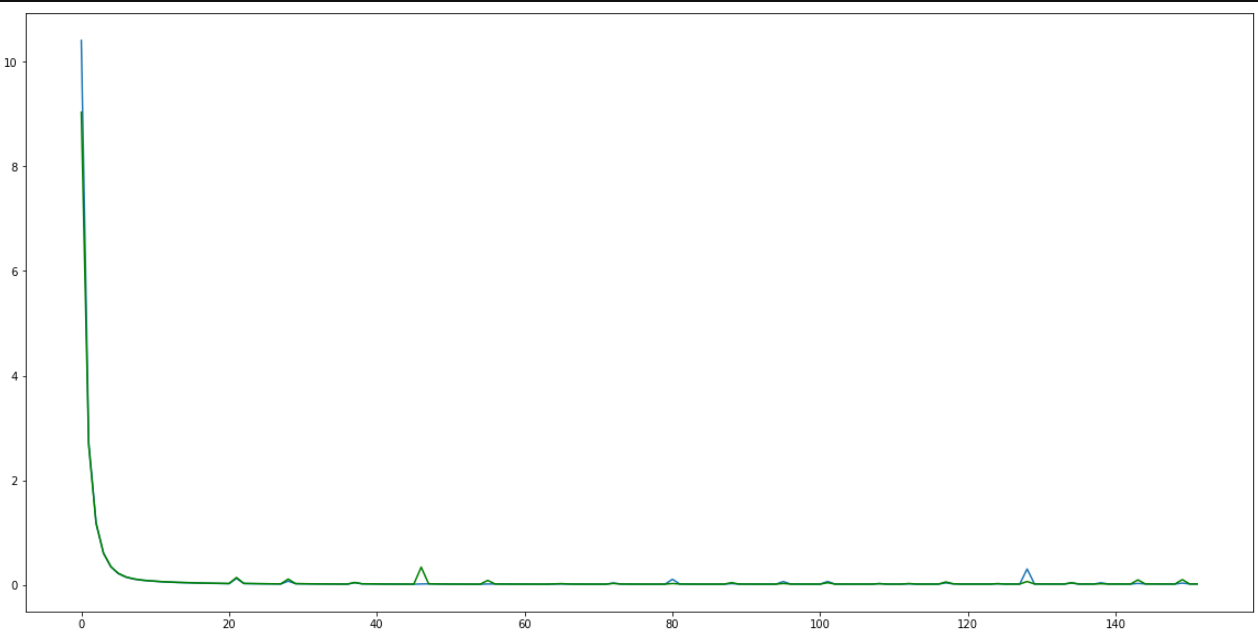
\includegraphics{img/1.png}
\end{itemize}

\paragraph{For 4 neuron learning
curve}\label{for-4-neuron-learning-curve}

\begin{itemize}
\tightlist
\item
  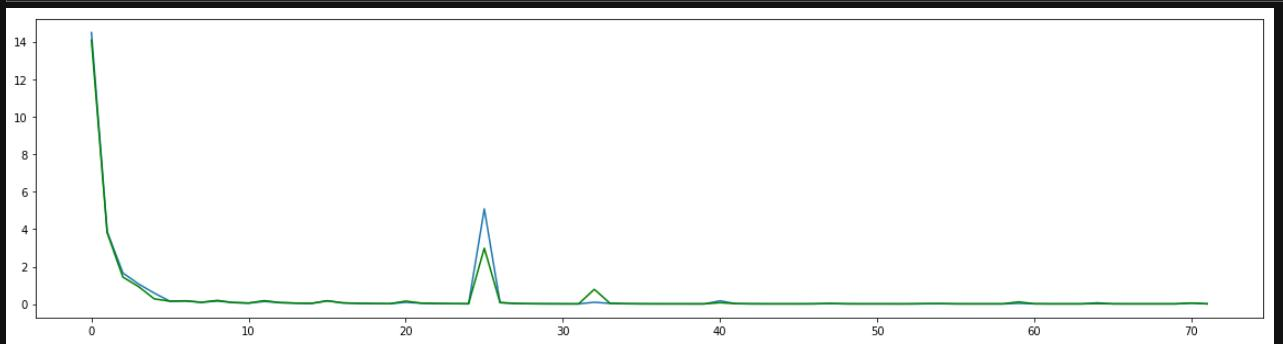
\includegraphics{img/4.png}
\end{itemize}

\paragraph{For 16 neuron learning
curve}\label{for-16-neuron-learning-curve}

\begin{itemize}
\tightlist
\item
  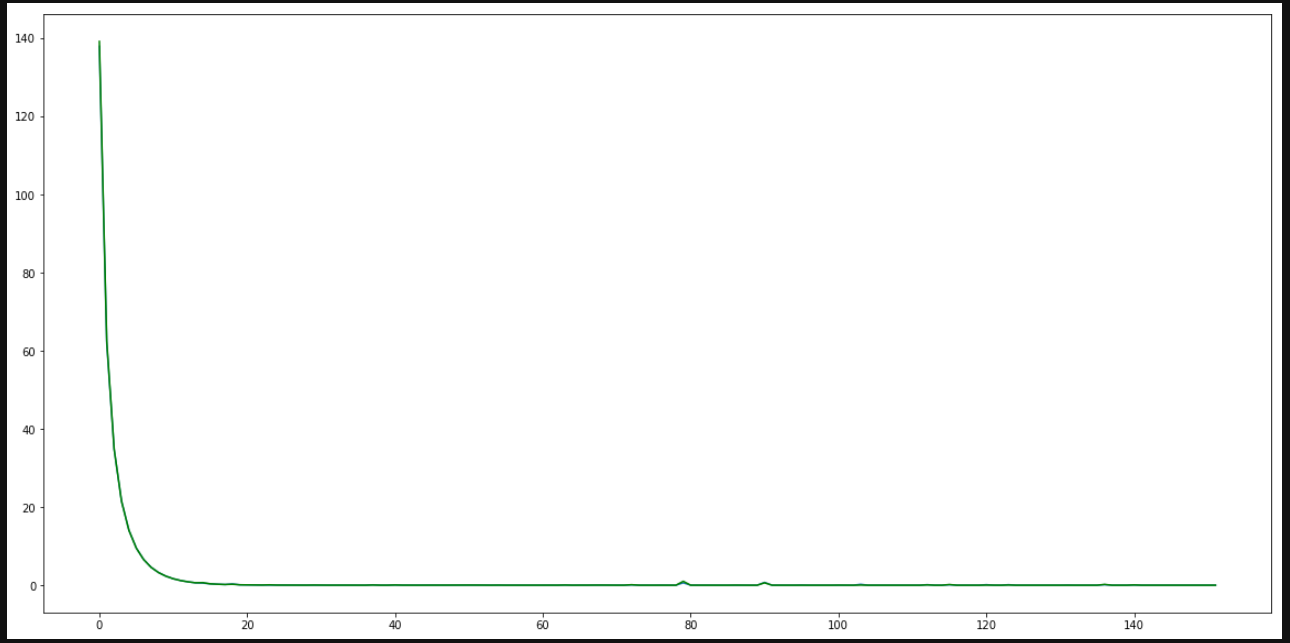
\includegraphics{img/16.png}
\end{itemize}

\paragraph{For 32 neuron learning
curve}\label{for-32-neuron-learning-curve}

\begin{itemize}
\item
  \begin{figure}
  \centering
  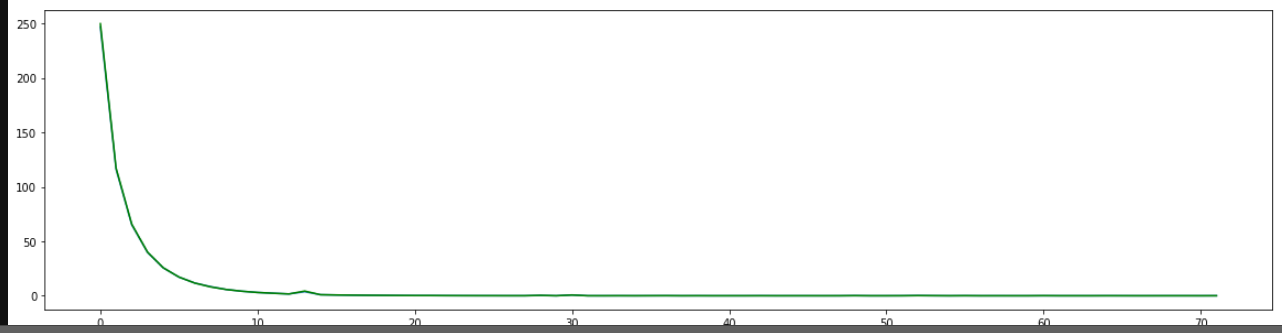
\includegraphics{img/32.png}
  \caption{alt text}
  \end{figure}
\item
  From the above graph we can say that for single neuron learning curve
  is not very stable but when neuron increases upto 32 that curve become
  smoother. But when submitted to kaggle 16 neuron performs better than
  32 and 4 so choosing it over others is helpful.
\end{itemize}

 

    \section{Ensemble}\label{ensemble}

I am using bagging method for this section. Usually in this technique we
add different models results and average them. But instead of averaging
I am taking different fraction from different models result. Finally
making sure that it sums up to 1.

    I have tried different combinations of ensemble learning to improve
performance. Kaggle has a certain limitation on uploading submission
files. So what I have tried is that before submitting it to kaggle, I
have made 80-20 split. I made prediction on the 20\% data. Then I have
tried ensemble learning so that before submission I can confirm which
combination might work well.

    Following 3 section arranges diffrent prediction results for ensembling.

    \begin{Verbatim}[commandchars=\\\{\}]
{\color{incolor}In [{\color{incolor}229}]:} \PY{n}{x} \PY{o}{=} \PY{p}{[}\PY{l+s+s1}{\PYZsq{}}\PY{l+s+s1}{Random Forest Regressor}\PY{l+s+s1}{\PYZsq{}}\PY{p}{,}
               \PY{l+s+s1}{\PYZsq{}}\PY{l+s+s1}{DecisionTree}\PY{l+s+s1}{\PYZsq{}}\PY{p}{,}\PY{l+s+s1}{\PYZsq{}}\PY{l+s+s1}{Xgboost}\PY{l+s+s1}{\PYZsq{}}\PY{p}{,}\PY{l+s+s1}{\PYZsq{}}\PY{l+s+s1}{Lasso}\PY{l+s+s1}{\PYZsq{}}\PY{p}{,}
               \PY{l+s+s1}{\PYZsq{}}\PY{l+s+s1}{ANN\PYZus{}base\PYZus{}lr0.1\PYZus{}beta0.1\PYZhy{}0.0\PYZhy{}0.0\PYZhy{}None\PYZus{}hidden16\PYZhy{}8\PYZhy{}4\PYZhy{}None}\PY{l+s+s1}{\PYZsq{}}\PY{p}{,}
               \PY{l+s+s1}{\PYZsq{}}\PY{l+s+s1}{ANN\PYZus{}lr0.1\PYZus{}beta0.1\PYZhy{}0.05\PYZhy{}0.0\PYZhy{}0.0\PYZus{}hidden76\PYZhy{}48\PYZhy{}32\PYZhy{}16}\PY{l+s+s1}{\PYZsq{}}\PY{p}{,}
               \PY{l+s+s1}{\PYZsq{}}\PY{l+s+s1}{ANN\PYZus{}lr0.05\PYZus{}beta0.005\PYZhy{}0.1\PYZhy{}0.05\PYZhy{}0.0\PYZus{}hidden8\PYZhy{}32\PYZhy{}16\PYZhy{}8}\PY{l+s+s1}{\PYZsq{}}\PY{p}{,}
               \PY{l+s+s1}{\PYZsq{}}\PY{l+s+s1}{ANN\PYZus{}lr0.05\PYZus{}beta0.1\PYZhy{}0.0\PYZhy{}0.0\PYZhy{}0.0\PYZus{}hidden16\PYZhy{}8\PYZhy{}4\PYZhy{}2}\PY{l+s+s1}{\PYZsq{}}\PY{p}{,}
               \PY{l+s+s1}{\PYZsq{}}\PY{l+s+s1}{ANN\PYZus{}lr0.1\PYZus{}beta0.1\PYZhy{}None\PYZhy{}None\PYZhy{}None\PYZus{}hidden16\PYZhy{}None\PYZhy{}None\PYZhy{}None}\PY{l+s+s1}{\PYZsq{}}\PY{p}{,}
               \PY{l+s+s1}{\PYZsq{}}\PY{l+s+s1}{ANN\PYZus{}lr0.1\PYZus{}beta0\PYZhy{}None\PYZhy{}None\PYZhy{}None\PYZus{}hidden4\PYZhy{}None\PYZhy{}None\PYZhy{}None}\PY{l+s+s1}{\PYZsq{}}\PY{p}{,}
               \PY{l+s+s1}{\PYZsq{}}\PY{l+s+s1}{ANN\PYZus{}lr0.1\PYZus{}beta0\PYZhy{}None\PYZhy{}None\PYZhy{}None\PYZus{}hidden2\PYZhy{}None\PYZhy{}None\PYZhy{}None}\PY{l+s+s1}{\PYZsq{}}\PY{p}{]}
\end{Verbatim}

    \begin{Verbatim}[commandchars=\\\{\}]
{\color{incolor}In [{\color{incolor}230}]:} \PY{n}{d} \PY{o}{=} \PY{n+nb}{dict}\PY{p}{(}\PY{p}{)}
          \PY{k}{for} \PY{n}{k} \PY{o+ow}{in} \PY{n}{x}\PY{p}{:}
              \PY{n}{d}\PY{p}{[}\PY{n}{k}\PY{p}{]} \PY{o}{=} \PY{n}{prediction\PYZus{}dict}\PY{p}{[}\PY{n}{k}\PY{p}{]}
          \PY{n}{prediction\PYZus{}dict} \PY{o}{=} \PY{n}{d}
\end{Verbatim}

    \begin{Verbatim}[commandchars=\\\{\}]
{\color{incolor}In [{\color{incolor}231}]:} \PY{k}{if} \PY{n}{submit} \PY{p}{:}
              \PY{n}{pred\PYZus{}df} \PY{o}{=} \PY{n}{pd}\PY{o}{.}\PY{n}{read\PYZus{}csv}\PY{p}{(}\PY{l+s+s2}{\PYZdq{}}\PY{l+s+s2}{diffrent\PYZus{}pred\PYZus{}results.csv}\PY{l+s+s2}{\PYZdq{}}\PY{p}{)}
          \PY{k}{else}\PY{p}{:}
              \PY{n}{pred\PYZus{}df} \PY{o}{=} \PY{n}{pd}\PY{o}{.}\PY{n}{read\PYZus{}csv}\PY{p}{(}\PY{l+s+s2}{\PYZdq{}}\PY{l+s+s2}{pred\PYZus{}results.csv}\PY{l+s+s2}{\PYZdq{}}\PY{p}{)}
              
              
          \PY{k}{if} \PY{o+ow}{not} \PY{n}{submit}\PY{p}{:}
              \PY{n}{pd}\PY{o}{.}\PY{n}{set\PYZus{}option}\PY{p}{(}\PY{l+s+s1}{\PYZsq{}}\PY{l+s+s1}{display.max\PYZus{}colwidth}\PY{l+s+s1}{\PYZsq{}}\PY{p}{,} \PY{o}{\PYZhy{}}\PY{l+m+mi}{1}\PY{p}{)}
              \PY{n}{pred\PYZus{}df} \PY{o}{=} \PY{n}{pd}\PY{o}{.}\PY{n}{DataFrame}\PY{p}{(}\PY{n}{prediction\PYZus{}dict}\PY{p}{)}
              \PY{n}{pred\PYZus{}df}\PY{o}{.}\PY{n}{to\PYZus{}csv}\PY{p}{(}\PY{l+s+s2}{\PYZdq{}}\PY{l+s+s2}{pred\PYZus{}results.csv}\PY{l+s+s2}{\PYZdq{}}\PY{p}{,} \PY{n}{encoding}\PY{o}{=}\PY{l+s+s1}{\PYZsq{}}\PY{l+s+s1}{utf\PYZhy{}8}\PY{l+s+s1}{\PYZsq{}}\PY{p}{,}\PY{n}{index}\PY{o}{=}\PY{k+kc}{False}\PY{p}{)}
          
          \PY{k}{else}\PY{p}{:}
              \PY{n}{pd}\PY{o}{.}\PY{n}{set\PYZus{}option}\PY{p}{(}\PY{l+s+s1}{\PYZsq{}}\PY{l+s+s1}{display.max\PYZus{}colwidth}\PY{l+s+s1}{\PYZsq{}}\PY{p}{,} \PY{o}{\PYZhy{}}\PY{l+m+mi}{1}\PY{p}{)}
              \PY{n}{pred\PYZus{}df} \PY{o}{=} \PY{n}{pd}\PY{o}{.}\PY{n}{DataFrame}\PY{p}{(}\PY{n}{submit\PYZus{}prediction\PYZus{}dict}\PY{p}{)}
              \PY{n}{pred\PYZus{}df}\PY{o}{.}\PY{n}{to\PYZus{}csv}\PY{p}{(}\PY{l+s+s2}{\PYZdq{}}\PY{l+s+s2}{diffrent\PYZus{}pred\PYZus{}results.csv}\PY{l+s+s2}{\PYZdq{}}\PY{p}{,} \PY{n}{encoding}\PY{o}{=}\PY{l+s+s1}{\PYZsq{}}\PY{l+s+s1}{utf\PYZhy{}8}\PY{l+s+s1}{\PYZsq{}}\PY{p}{,}\PY{n}{index}\PY{o}{=}\PY{k+kc}{False}\PY{p}{)}
          
          \PY{n}{pd}\PY{o}{.}\PY{n}{DataFrame}\PY{p}{(}\PY{n}{pred\PYZus{}df}\PY{o}{.}\PY{n}{columns}\PY{p}{)}
\end{Verbatim}

\begin{Verbatim}[commandchars=\\\{\}]
{\color{outcolor}Out[{\color{outcolor}231}]:}                                                            0
          0   Random Forest Regressor                                 
          1   DecisionTree                                            
          2   Xgboost                                                 
          3   Lasso                                                   
          4   ANN\_base\_lr0.1\_beta0.1-0.0-0.0-None\_hidden16-8-4-None   
          5   ANN\_lr0.1\_beta0.1-0.05-0.0-0.0\_hidden76-48-32-16        
          6   ANN\_lr0.05\_beta0.005-0.1-0.05-0.0\_hidden8-32-16-8       
          7   ANN\_lr0.05\_beta0.1-0.0-0.0-0.0\_hidden16-8-4-2           
          8   ANN\_lr0.1\_beta0.1-None-None-None\_hidden16-None-None-None
          9   ANN\_lr0.1\_beta0-None-None-None\_hidden4-None-None-None   
          10  ANN\_lr0.1\_beta0-None-None-None\_hidden2-None-None-None   
\end{Verbatim}
            
    \subsubsection{Naming explanation of above
table}\label{naming-explanation-of-above-table}

\begin{longtable}[]{@{}llllllllll@{}}
\toprule
\begin{minipage}[b]{0.04\columnwidth}\raggedright\strut
Name\strut
\end{minipage} & \begin{minipage}[b]{0.09\columnwidth}\raggedright\strut
learning rate\strut
\end{minipage} & \begin{minipage}[b]{0.04\columnwidth}\raggedright\strut
beta1\strut
\end{minipage} & \begin{minipage}[b]{0.05\columnwidth}\raggedright\strut
beta 2\strut
\end{minipage} & \begin{minipage}[b]{0.05\columnwidth}\raggedright\strut
beta 3\strut
\end{minipage} & \begin{minipage}[b]{0.05\columnwidth}\raggedright\strut
beta 4\strut
\end{minipage} & \begin{minipage}[b]{0.10\columnwidth}\raggedright\strut
hidden layer 1\strut
\end{minipage} & \begin{minipage}[b]{0.10\columnwidth}\raggedright\strut
hidden layer 2\strut
\end{minipage} & \begin{minipage}[b]{0.09\columnwidth}\raggedright\strut
hidden layer 3\strut
\end{minipage} & \begin{minipage}[b]{0.11\columnwidth}\raggedright\strut
hidden layer 4\strut
\end{minipage}\tabularnewline
\midrule
\endhead
\begin{minipage}[t]{0.04\columnwidth}\raggedright\strut
ANN\_base\_lr0.1\_beta0.1-0.0-0.0-None\_hidden16-8-4-None\strut
\end{minipage} & \begin{minipage}[t]{0.09\columnwidth}\raggedright\strut
0.1\strut
\end{minipage} & \begin{minipage}[t]{0.04\columnwidth}\raggedright\strut
0.1\strut
\end{minipage} & \begin{minipage}[t]{0.05\columnwidth}\raggedright\strut
0.0\strut
\end{minipage} & \begin{minipage}[t]{0.05\columnwidth}\raggedright\strut
0.0\strut
\end{minipage} & \begin{minipage}[t]{0.05\columnwidth}\raggedright\strut
None\strut
\end{minipage} & \begin{minipage}[t]{0.10\columnwidth}\raggedright\strut
16\strut
\end{minipage} & \begin{minipage}[t]{0.10\columnwidth}\raggedright\strut
8\strut
\end{minipage} & \begin{minipage}[t]{0.09\columnwidth}\raggedright\strut
4\strut
\end{minipage} & \begin{minipage}[t]{0.11\columnwidth}\raggedright\strut
None\strut
\end{minipage}\tabularnewline
\begin{minipage}[t]{0.04\columnwidth}\raggedright\strut
ANN\_lr0.05\_beta0.005-0.1-0.05-0.0\_hidden8-32-16-8\strut
\end{minipage} & \begin{minipage}[t]{0.09\columnwidth}\raggedright\strut
0.05\strut
\end{minipage} & \begin{minipage}[t]{0.04\columnwidth}\raggedright\strut
0.005\strut
\end{minipage} & \begin{minipage}[t]{0.05\columnwidth}\raggedright\strut
0.1\strut
\end{minipage} & \begin{minipage}[t]{0.05\columnwidth}\raggedright\strut
0.05\strut
\end{minipage} & \begin{minipage}[t]{0.05\columnwidth}\raggedright\strut
0\strut
\end{minipage} & \begin{minipage}[t]{0.10\columnwidth}\raggedright\strut
8\strut
\end{minipage} & \begin{minipage}[t]{0.10\columnwidth}\raggedright\strut
32\strut
\end{minipage} & \begin{minipage}[t]{0.09\columnwidth}\raggedright\strut
16\strut
\end{minipage} & \begin{minipage}[t]{0.11\columnwidth}\raggedright\strut
6\strut
\end{minipage}\tabularnewline
\begin{minipage}[t]{0.04\columnwidth}\raggedright\strut
ANN\_lr0.05\_beta0.1-0.0-0.0-0.0\_hidden16-8-4-2\strut
\end{minipage} & \begin{minipage}[t]{0.09\columnwidth}\raggedright\strut
.05\strut
\end{minipage} & \begin{minipage}[t]{0.04\columnwidth}\raggedright\strut
0.1\strut
\end{minipage} & \begin{minipage}[t]{0.05\columnwidth}\raggedright\strut
0.0\strut
\end{minipage} & \begin{minipage}[t]{0.05\columnwidth}\raggedright\strut
0.0\strut
\end{minipage} & \begin{minipage}[t]{0.05\columnwidth}\raggedright\strut
0.0\strut
\end{minipage} & \begin{minipage}[t]{0.10\columnwidth}\raggedright\strut
16\strut
\end{minipage} & \begin{minipage}[t]{0.10\columnwidth}\raggedright\strut
8\strut
\end{minipage} & \begin{minipage}[t]{0.09\columnwidth}\raggedright\strut
4\strut
\end{minipage} & \begin{minipage}[t]{0.11\columnwidth}\raggedright\strut
2\strut
\end{minipage}\tabularnewline
\begin{minipage}[t]{0.04\columnwidth}\raggedright\strut
ANN\_lr0.1\_beta0-None-None-None\_hidden2-None-None-None\strut
\end{minipage} & \begin{minipage}[t]{0.09\columnwidth}\raggedright\strut
0.1\strut
\end{minipage} & \begin{minipage}[t]{0.04\columnwidth}\raggedright\strut
0\strut
\end{minipage} & \begin{minipage}[t]{0.05\columnwidth}\raggedright\strut
None\strut
\end{minipage} & \begin{minipage}[t]{0.05\columnwidth}\raggedright\strut
None\strut
\end{minipage} & \begin{minipage}[t]{0.05\columnwidth}\raggedright\strut
None\strut
\end{minipage} & \begin{minipage}[t]{0.10\columnwidth}\raggedright\strut
2\strut
\end{minipage} & \begin{minipage}[t]{0.10\columnwidth}\raggedright\strut
None\strut
\end{minipage} & \begin{minipage}[t]{0.09\columnwidth}\raggedright\strut
None\strut
\end{minipage} & \begin{minipage}[t]{0.11\columnwidth}\raggedright\strut
None\strut
\end{minipage}\tabularnewline
\begin{minipage}[t]{0.04\columnwidth}\raggedright\strut
ANN\_lr0.1\_beta0.1-0.05-0.0-0.0\_hidden76-48-32-16\strut
\end{minipage} & \begin{minipage}[t]{0.09\columnwidth}\raggedright\strut
0.1\strut
\end{minipage} & \begin{minipage}[t]{0.04\columnwidth}\raggedright\strut
.1\strut
\end{minipage} & \begin{minipage}[t]{0.05\columnwidth}\raggedright\strut
0.05\strut
\end{minipage} & \begin{minipage}[t]{0.05\columnwidth}\raggedright\strut
0.0\strut
\end{minipage} & \begin{minipage}[t]{0.05\columnwidth}\raggedright\strut
0.0\strut
\end{minipage} & \begin{minipage}[t]{0.10\columnwidth}\raggedright\strut
76\strut
\end{minipage} & \begin{minipage}[t]{0.10\columnwidth}\raggedright\strut
48\strut
\end{minipage} & \begin{minipage}[t]{0.09\columnwidth}\raggedright\strut
32\strut
\end{minipage} & \begin{minipage}[t]{0.11\columnwidth}\raggedright\strut
16\strut
\end{minipage}\tabularnewline
\begin{minipage}[t]{0.04\columnwidth}\raggedright\strut
ANN\_lr0.1\_beta0.1-None-None-None\_hidden16-None-None-None\strut
\end{minipage} & \begin{minipage}[t]{0.09\columnwidth}\raggedright\strut
0.1\strut
\end{minipage} & \begin{minipage}[t]{0.04\columnwidth}\raggedright\strut
0.1\strut
\end{minipage} & \begin{minipage}[t]{0.05\columnwidth}\raggedright\strut
None\strut
\end{minipage} & \begin{minipage}[t]{0.05\columnwidth}\raggedright\strut
None\strut
\end{minipage} & \begin{minipage}[t]{0.05\columnwidth}\raggedright\strut
None\strut
\end{minipage} & \begin{minipage}[t]{0.10\columnwidth}\raggedright\strut
16\strut
\end{minipage} & \begin{minipage}[t]{0.10\columnwidth}\raggedright\strut
None\strut
\end{minipage} & \begin{minipage}[t]{0.09\columnwidth}\raggedright\strut
None\strut
\end{minipage} & \begin{minipage}[t]{0.11\columnwidth}\raggedright\strut
None\strut
\end{minipage}\tabularnewline
\begin{minipage}[t]{0.04\columnwidth}\raggedright\strut
ANN\_lr0.1\_beta0-None-None-None\_hidden4-None-None-None\strut
\end{minipage} & \begin{minipage}[t]{0.09\columnwidth}\raggedright\strut
0.1\strut
\end{minipage} & \begin{minipage}[t]{0.04\columnwidth}\raggedright\strut
0\strut
\end{minipage} & \begin{minipage}[t]{0.05\columnwidth}\raggedright\strut
None\strut
\end{minipage} & \begin{minipage}[t]{0.05\columnwidth}\raggedright\strut
None\strut
\end{minipage} & \begin{minipage}[t]{0.05\columnwidth}\raggedright\strut
None\strut
\end{minipage} & \begin{minipage}[t]{0.10\columnwidth}\raggedright\strut
4\strut
\end{minipage} & \begin{minipage}[t]{0.10\columnwidth}\raggedright\strut
None\strut
\end{minipage} & \begin{minipage}[t]{0.09\columnwidth}\raggedright\strut
None\strut
\end{minipage} & \begin{minipage}[t]{0.11\columnwidth}\raggedright\strut
None\strut
\end{minipage}\tabularnewline
\bottomrule
\end{longtable}

    \paragraph{Ensemble Combination 1}\label{ensemble-combination-1}

    \begin{Verbatim}[commandchars=\\\{\}]
{\color{incolor}In [{\color{incolor}232}]:} \PY{c+c1}{\PYZsh{} pred\PYZus{}df[pred\PYZus{}df.columns[[1,3,5]]] * [1,2,30]}
          
          \PY{n+nb}{print}\PY{p}{(}\PY{l+s+s1}{\PYZsq{}}\PY{l+s+s1}{Using  }\PY{l+s+s1}{\PYZsq{}} \PY{p}{,} \PY{n}{pred\PYZus{}df}\PY{o}{.}\PY{n}{columns}\PY{p}{[}\PY{p}{[}\PY{l+m+mi}{4}\PY{p}{,}\PY{l+m+mi}{3}\PY{p}{,}\PY{l+m+mi}{2}\PY{p}{]}\PY{p}{]}\PY{o}{.}\PY{n}{values}\PY{p}{)}
\end{Verbatim}

    \begin{Verbatim}[commandchars=\\\{\}]
Using   ['ANN\_base\_lr0.1\_beta0.1-0.0-0.0-None\_hidden16-8-4-None' 'Lasso' 'Xgboost']

    \end{Verbatim}

    \begin{Verbatim}[commandchars=\\\{\}]
{\color{incolor}In [{\color{incolor}233}]:} \PY{n}{prediction} \PY{o}{=} \PY{n}{pred\PYZus{}df}\PY{p}{[}\PY{n}{pred\PYZus{}df}\PY{o}{.}\PY{n}{columns}\PY{p}{[}\PY{p}{[}\PY{l+m+mi}{4}\PY{p}{,}\PY{l+m+mi}{3}\PY{p}{,}\PY{l+m+mi}{2}\PY{p}{]}\PY{p}{]}\PY{p}{]} \PY{o}{*} \PY{p}{[}\PY{o}{.}\PY{l+m+mi}{4}\PY{p}{,}\PY{o}{.}\PY{l+m+mi}{2}\PY{p}{,}\PY{o}{.}\PY{l+m+mi}{4}\PY{p}{]}
          \PY{n}{prediction} \PY{o}{=} \PY{n}{prediction}\PY{o}{.}\PY{n}{sum}\PY{p}{(}\PY{n}{axis} \PY{o}{=} \PY{l+m+mi}{1}\PY{p}{)}
          
          \PY{k}{if} \PY{o+ow}{not} \PY{n}{submit}\PY{p}{:}
              \PY{n}{test\PYZus{}rmse\PYZus{}score}\PY{p}{,} \PY{n}{test\PYZus{}r2\PYZus{}score} \PY{o}{=} \PY{n}{accuracy}\PY{p}{(}\PY{n}{y\PYZus{}val}\PY{p}{,} \PY{n}{prediction}\PY{p}{)}
          
              \PY{n+nb}{print}\PY{p}{(}\PY{l+s+s1}{\PYZsq{}}\PY{l+s+s1}{ann root mean absolute error: }\PY{l+s+s1}{\PYZsq{}}\PY{p}{,} \PY{n}{test\PYZus{}rmse\PYZus{}score}\PY{p}{)}
              \PY{n+nb}{print}\PY{p}{(}\PY{l+s+s1}{\PYZsq{}}\PY{l+s+s1}{accuracy score: }\PY{l+s+s1}{\PYZsq{}}\PY{p}{,} \PY{n}{test\PYZus{}r2\PYZus{}score}  \PY{p}{)}
\end{Verbatim}

    \begin{Verbatim}[commandchars=\\\{\}]
ann root mean absolute error:  0.10075045445576623
accuracy score:  0.9401051461891021

    \end{Verbatim}

    \subparagraph{Kaggle score}\label{kaggle-score}

\begin{itemize}
\tightlist
\item
  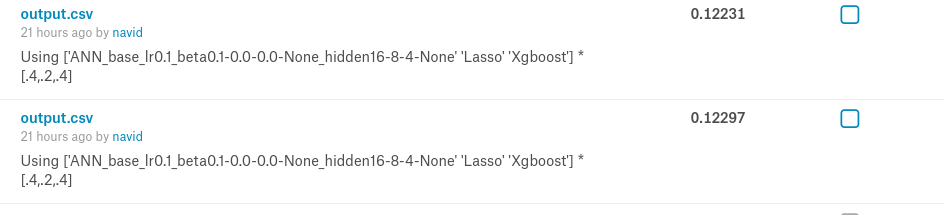
\includegraphics{img/ensemble3xg.png}
\end{itemize}

    \begin{Verbatim}[commandchars=\\\{\}]
{\color{incolor}In [{\color{incolor}234}]:} \PY{n}{prediction} \PY{o}{=} \PY{n}{pred\PYZus{}df}\PY{p}{[}\PY{n}{pred\PYZus{}df}\PY{o}{.}\PY{n}{columns}\PY{p}{[}\PY{p}{[}\PY{l+m+mi}{4}\PY{p}{,}\PY{l+m+mi}{3}\PY{p}{,}\PY{l+m+mi}{2}\PY{p}{]}\PY{p}{]}\PY{p}{]} \PY{o}{*} \PY{p}{[}\PY{o}{.}\PY{l+m+mi}{4}\PY{p}{,}\PY{o}{.}\PY{l+m+mi}{3}\PY{p}{,}\PY{o}{.}\PY{l+m+mi}{3}\PY{p}{]}
          \PY{n}{prediction} \PY{o}{=} \PY{n}{prediction}\PY{o}{.}\PY{n}{sum}\PY{p}{(}\PY{n}{axis} \PY{o}{=} \PY{l+m+mi}{1}\PY{p}{)}
          
          \PY{k}{if} \PY{o+ow}{not} \PY{n}{submit}\PY{p}{:}
              \PY{n}{test\PYZus{}rmse\PYZus{}score}\PY{p}{,} \PY{n}{test\PYZus{}r2\PYZus{}score} \PY{o}{=} \PY{n}{accuracy}\PY{p}{(}\PY{n}{y\PYZus{}val}\PY{p}{,} \PY{n}{prediction}\PY{p}{)}
          
              \PY{n+nb}{print}\PY{p}{(}\PY{l+s+s1}{\PYZsq{}}\PY{l+s+s1}{ann root mean absolute error: }\PY{l+s+s1}{\PYZsq{}}\PY{p}{,} \PY{n}{test\PYZus{}rmse\PYZus{}score}\PY{p}{)}
              \PY{n+nb}{print}\PY{p}{(}\PY{l+s+s1}{\PYZsq{}}\PY{l+s+s1}{accuracy score: }\PY{l+s+s1}{\PYZsq{}}\PY{p}{,} \PY{n}{test\PYZus{}r2\PYZus{}score}  \PY{p}{)}
\end{Verbatim}

    \begin{Verbatim}[commandchars=\\\{\}]
ann root mean absolute error:  0.10101768287528032
accuracy score:  0.9397869970814289

    \end{Verbatim}

    \paragraph{Ensemble Combination 2}\label{ensemble-combination-2}

    \begin{Verbatim}[commandchars=\\\{\}]
{\color{incolor}In [{\color{incolor}235}]:} \PY{c+c1}{\PYZsh{} pred\PYZus{}df[pred\PYZus{}df.columns[[1,3,5]]] * [1,2,30]}
          
          \PY{n+nb}{print}\PY{p}{(}\PY{l+s+s1}{\PYZsq{}}\PY{l+s+s1}{Using  }\PY{l+s+s1}{\PYZsq{}} \PY{p}{,} \PY{n}{pred\PYZus{}df}\PY{o}{.}\PY{n}{columns}\PY{p}{[}\PY{p}{[}\PY{l+m+mi}{2}\PY{p}{,}\PY{l+m+mi}{4}\PY{p}{,}\PY{l+m+mi}{5}\PY{p}{,}\PY{l+m+mi}{6}\PY{p}{,}\PY{l+m+mi}{7}\PY{p}{]}\PY{p}{]}\PY{o}{.}\PY{n}{values}\PY{p}{)}
\end{Verbatim}

    \begin{Verbatim}[commandchars=\\\{\}]
Using   ['Xgboost' 'ANN\_base\_lr0.1\_beta0.1-0.0-0.0-None\_hidden16-8-4-None'
 'ANN\_lr0.1\_beta0.1-0.05-0.0-0.0\_hidden76-48-32-16'
 'ANN\_lr0.05\_beta0.005-0.1-0.05-0.0\_hidden8-32-16-8'
 'ANN\_lr0.05\_beta0.1-0.0-0.0-0.0\_hidden16-8-4-2']

    \end{Verbatim}

    \begin{Verbatim}[commandchars=\\\{\}]
{\color{incolor}In [{\color{incolor}236}]:} \PY{n}{prediction} \PY{o}{=} \PY{n}{pred\PYZus{}df}\PY{p}{[}\PY{n}{pred\PYZus{}df}\PY{o}{.}\PY{n}{columns}\PY{p}{[}\PY{p}{[}\PY{l+m+mi}{2}\PY{p}{,}\PY{l+m+mi}{4}\PY{p}{,}\PY{l+m+mi}{5}\PY{p}{,}\PY{l+m+mi}{6}\PY{p}{,}\PY{l+m+mi}{7}\PY{p}{]}\PY{p}{]}\PY{p}{]} \PY{o}{*} \PY{p}{[}\PY{o}{.}\PY{l+m+mi}{25}\PY{p}{,}\PY{o}{.}\PY{l+m+mi}{2}\PY{p}{,}\PY{o}{.}\PY{l+m+mi}{2} \PY{p}{,}\PY{o}{.}\PY{l+m+mi}{15} \PY{p}{,} \PY{o}{.}\PY{l+m+mi}{2}\PY{p}{]}
          \PY{n}{prediction} \PY{o}{=} \PY{n}{prediction}\PY{o}{.}\PY{n}{sum}\PY{p}{(}\PY{n}{axis} \PY{o}{=} \PY{l+m+mi}{1}\PY{p}{)}
          
          \PY{k}{if} \PY{o+ow}{not} \PY{n}{submit}\PY{p}{:}
              \PY{n}{test\PYZus{}rmse\PYZus{}score}\PY{p}{,} \PY{n}{test\PYZus{}r2\PYZus{}score} \PY{o}{=} \PY{n}{accuracy}\PY{p}{(}\PY{n}{y\PYZus{}val}\PY{p}{,} \PY{n}{prediction}\PY{p}{)}
          
              \PY{n+nb}{print}\PY{p}{(}\PY{l+s+s1}{\PYZsq{}}\PY{l+s+s1}{ann root mean absolute error: }\PY{l+s+s1}{\PYZsq{}}\PY{p}{,} \PY{n}{test\PYZus{}rmse\PYZus{}score}\PY{p}{)}
              \PY{n+nb}{print}\PY{p}{(}\PY{l+s+s1}{\PYZsq{}}\PY{l+s+s1}{accuracy score: }\PY{l+s+s1}{\PYZsq{}}\PY{p}{,} \PY{n}{test\PYZus{}r2\PYZus{}score}  \PY{p}{)}
\end{Verbatim}

    \begin{Verbatim}[commandchars=\\\{\}]
ann root mean absolute error:  0.09941663280977221
accuracy score:  0.9416805283100553

    \end{Verbatim}

    \subparagraph{Kaggle score}\label{kaggle-score}

\begin{itemize}
\tightlist
\item
  
\includegraphics{img/annxgb.png}
\end{itemize}

    \paragraph{Ensemble Combination 3}\label{ensemble-combination-3}

    \begin{Verbatim}[commandchars=\\\{\}]
{\color{incolor}In [{\color{incolor}237}]:} \PY{n+nb}{print}\PY{p}{(}\PY{l+s+s1}{\PYZsq{}}\PY{l+s+s1}{Using  }\PY{l+s+s1}{\PYZsq{}} \PY{p}{,} \PY{n}{pred\PYZus{}df}\PY{o}{.}\PY{n}{columns}\PY{p}{[}\PY{p}{[}\PY{l+m+mi}{0}\PY{p}{,}\PY{l+m+mi}{4}\PY{p}{,}\PY{l+m+mi}{5}\PY{p}{,}\PY{l+m+mi}{6}\PY{p}{,}\PY{l+m+mi}{7}\PY{p}{]}\PY{p}{]}\PY{o}{.}\PY{n}{values}\PY{p}{)}
\end{Verbatim}

    \begin{Verbatim}[commandchars=\\\{\}]
Using   ['Random Forest Regressor'
 'ANN\_base\_lr0.1\_beta0.1-0.0-0.0-None\_hidden16-8-4-None'
 'ANN\_lr0.1\_beta0.1-0.05-0.0-0.0\_hidden76-48-32-16'
 'ANN\_lr0.05\_beta0.005-0.1-0.05-0.0\_hidden8-32-16-8'
 'ANN\_lr0.05\_beta0.1-0.0-0.0-0.0\_hidden16-8-4-2']

    \end{Verbatim}

    \begin{Verbatim}[commandchars=\\\{\}]
{\color{incolor}In [{\color{incolor}238}]:} \PY{n}{prediction} \PY{o}{=} \PY{n}{pred\PYZus{}df}\PY{p}{[}\PY{n}{pred\PYZus{}df}\PY{o}{.}\PY{n}{columns}\PY{p}{[}\PY{p}{[}\PY{l+m+mi}{0}\PY{p}{,}\PY{l+m+mi}{4}\PY{p}{,}\PY{l+m+mi}{5}\PY{p}{,}\PY{l+m+mi}{6}\PY{p}{,}\PY{l+m+mi}{7}\PY{p}{]}\PY{p}{]}\PY{p}{]} \PY{o}{*} \PY{p}{[}\PY{o}{.}\PY{l+m+mi}{25}\PY{p}{,}\PY{o}{.}\PY{l+m+mi}{2}\PY{p}{,}\PY{o}{.}\PY{l+m+mi}{2} \PY{p}{,}\PY{o}{.}\PY{l+m+mi}{15} \PY{p}{,} \PY{o}{.}\PY{l+m+mi}{2}\PY{p}{]}
          \PY{n}{prediction} \PY{o}{=} \PY{n}{prediction}\PY{o}{.}\PY{n}{sum}\PY{p}{(}\PY{n}{axis} \PY{o}{=} \PY{l+m+mi}{1}\PY{p}{)}
          
          \PY{k}{if} \PY{o+ow}{not} \PY{n}{submit}\PY{p}{:}
              \PY{n}{test\PYZus{}rmse\PYZus{}score}\PY{p}{,} \PY{n}{test\PYZus{}r2\PYZus{}score} \PY{o}{=} \PY{n}{accuracy}\PY{p}{(}\PY{n}{y\PYZus{}val}\PY{p}{,} \PY{n}{prediction}\PY{p}{)}
          
              \PY{n+nb}{print}\PY{p}{(}\PY{l+s+s1}{\PYZsq{}}\PY{l+s+s1}{ann root mean absolute error: }\PY{l+s+s1}{\PYZsq{}}\PY{p}{,} \PY{n}{test\PYZus{}rmse\PYZus{}score}\PY{p}{)}
              \PY{n+nb}{print}\PY{p}{(}\PY{l+s+s1}{\PYZsq{}}\PY{l+s+s1}{accuracy score: }\PY{l+s+s1}{\PYZsq{}}\PY{p}{,} \PY{n}{test\PYZus{}r2\PYZus{}score}  \PY{p}{)}
\end{Verbatim}

    \begin{Verbatim}[commandchars=\\\{\}]
ann root mean absolute error:  0.1010286851201982
accuracy score:  0.9397738802831993

    \end{Verbatim}

    \subparagraph{Kaggle score}\label{kaggle-score}

\begin{itemize}
\tightlist
\item
  
\includegraphics{img/2522152.png}
\end{itemize}

    \paragraph{Ensemble Combination 4}\label{ensemble-combination-4}

    \begin{Verbatim}[commandchars=\\\{\}]
{\color{incolor}In [{\color{incolor}239}]:} \PY{n+nb}{print}\PY{p}{(}\PY{l+s+s1}{\PYZsq{}}\PY{l+s+s1}{Using  }\PY{l+s+s1}{\PYZsq{}} \PY{p}{,} \PY{n}{pred\PYZus{}df}\PY{o}{.}\PY{n}{columns}\PY{p}{[}\PY{p}{[}\PY{l+m+mi}{4}\PY{p}{,}\PY{l+m+mi}{5}\PY{p}{,}\PY{l+m+mi}{6}\PY{p}{,}\PY{l+m+mi}{7}\PY{p}{,}\PY{l+m+mi}{0}\PY{p}{,}\PY{l+m+mi}{2}\PY{p}{,}\PY{l+m+mi}{3}\PY{p}{]}\PY{p}{]}\PY{o}{.}\PY{n}{values}\PY{p}{)}
\end{Verbatim}

    \begin{Verbatim}[commandchars=\\\{\}]
Using   ['ANN\_base\_lr0.1\_beta0.1-0.0-0.0-None\_hidden16-8-4-None'
 'ANN\_lr0.1\_beta0.1-0.05-0.0-0.0\_hidden76-48-32-16'
 'ANN\_lr0.05\_beta0.005-0.1-0.05-0.0\_hidden8-32-16-8'
 'ANN\_lr0.05\_beta0.1-0.0-0.0-0.0\_hidden16-8-4-2' 'Random Forest Regressor'
 'Xgboost' 'Lasso']

    \end{Verbatim}

    \begin{Verbatim}[commandchars=\\\{\}]
{\color{incolor}In [{\color{incolor}240}]:} \PY{n}{prediction} \PY{o}{=} \PY{n}{pred\PYZus{}df}\PY{p}{[}\PY{n}{pred\PYZus{}df}\PY{o}{.}\PY{n}{columns}\PY{p}{[}\PY{p}{[}\PY{l+m+mi}{4}\PY{p}{,}\PY{l+m+mi}{5}\PY{p}{,}\PY{l+m+mi}{6}\PY{p}{,}\PY{l+m+mi}{7}\PY{p}{,}\PY{l+m+mi}{0}\PY{p}{,}\PY{l+m+mi}{2}\PY{p}{,}\PY{l+m+mi}{3}\PY{p}{]}\PY{p}{]}\PY{p}{]} \PY{o}{*} \PY{p}{[}\PY{o}{.}\PY{l+m+mi}{15}\PY{p}{,}\PY{o}{.}\PY{l+m+mi}{1}\PY{p}{,}\PY{o}{.}\PY{l+m+mi}{1}\PY{p}{,}\PY{o}{.}\PY{l+m+mi}{05}\PY{p}{,}\PY{o}{.}\PY{l+m+mi}{0}\PY{p}{,}\PY{o}{.}\PY{l+m+mi}{2}\PY{p}{,}\PY{o}{.}\PY{l+m+mi}{4}\PY{p}{]}
          \PY{n}{prediction} \PY{o}{=} \PY{n}{prediction}\PY{o}{.}\PY{n}{sum}\PY{p}{(}\PY{n}{axis} \PY{o}{=} \PY{l+m+mi}{1}\PY{p}{)}
          
          \PY{k}{if} \PY{o+ow}{not} \PY{n}{submit}\PY{p}{:}
              \PY{n}{test\PYZus{}rmse\PYZus{}score}\PY{p}{,} \PY{n}{test\PYZus{}r2\PYZus{}score} \PY{o}{=} \PY{n}{accuracy}\PY{p}{(}\PY{n}{y\PYZus{}val}\PY{p}{,} \PY{n}{prediction}\PY{p}{)}
          
              \PY{n+nb}{print}\PY{p}{(}\PY{l+s+s1}{\PYZsq{}}\PY{l+s+s1}{ann root mean absolute error: }\PY{l+s+s1}{\PYZsq{}}\PY{p}{,} \PY{n}{test\PYZus{}rmse\PYZus{}score}\PY{p}{)}
              \PY{n+nb}{print}\PY{p}{(}\PY{l+s+s1}{\PYZsq{}}\PY{l+s+s1}{accuracy score: }\PY{l+s+s1}{\PYZsq{}}\PY{p}{,} \PY{n}{test\PYZus{}r2\PYZus{}score}  \PY{p}{)}
\end{Verbatim}

    \begin{Verbatim}[commandchars=\\\{\}]
ann root mean absolute error:  0.1004754821798716
accuracy score:  0.9404316350340652

    \end{Verbatim}

    \subparagraph{Kaggle score}\label{kaggle-score}

\begin{itemize}
\tightlist
\item
  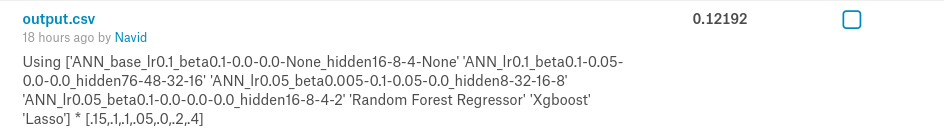
\includegraphics{img/kaggle_score.png}
\end{itemize}

    Ensemble combination 4 provides the best score which is 0.12192.
Currently combination 4 is showing that rmse value is .1004 and there is
a worse value present in combination 1 which is 0.1017. The reason
behind the difference is ANN does not perform exactly same each time.
That means if I currently submit with Combination 1 I might get better
results than Combination 4 .

In Combination 4 used models with their parameters:

\begin{longtable}[]{@{}lllllllllll@{}}
\toprule
\begin{minipage}[b]{0.04\columnwidth}\raggedright\strut
Name\strut
\end{minipage} & \begin{minipage}[b]{0.09\columnwidth}\raggedright\strut
learning rate\strut
\end{minipage} & \begin{minipage}[b]{0.04\columnwidth}\raggedright\strut
beta1\strut
\end{minipage} & \begin{minipage}[b]{0.05\columnwidth}\raggedright\strut
beta 2\strut
\end{minipage} & \begin{minipage}[b]{0.05\columnwidth}\raggedright\strut
beta 3\strut
\end{minipage} & \begin{minipage}[b]{0.05\columnwidth}\raggedright\strut
beta 4\strut
\end{minipage} & \begin{minipage}[b]{0.09\columnwidth}\raggedright\strut
hidden layer 1\strut
\end{minipage} & \begin{minipage}[b]{0.09\columnwidth}\raggedright\strut
hidden layer 2\strut
\end{minipage} & \begin{minipage}[b]{0.09\columnwidth}\raggedright\strut
hidden layer 3\strut
\end{minipage} & \begin{minipage}[b]{0.10\columnwidth}\raggedright\strut
hidden layer 4\strut
\end{minipage} & \begin{minipage}[b]{0.04\columnwidth}\raggedright\strut
Fraction taken\strut
\end{minipage}\tabularnewline
\midrule
\endhead
\begin{minipage}[t]{0.04\columnwidth}\raggedright\strut
ANN\_base\_lr0.1\_beta0.1-0.0-0.0-None\_hidden16-8-4-None\strut
\end{minipage} & \begin{minipage}[t]{0.09\columnwidth}\raggedright\strut
0.1\strut
\end{minipage} & \begin{minipage}[t]{0.04\columnwidth}\raggedright\strut
0.1\strut
\end{minipage} & \begin{minipage}[t]{0.05\columnwidth}\raggedright\strut
0.0\strut
\end{minipage} & \begin{minipage}[t]{0.05\columnwidth}\raggedright\strut
0.0\strut
\end{minipage} & \begin{minipage}[t]{0.05\columnwidth}\raggedright\strut
None\strut
\end{minipage} & \begin{minipage}[t]{0.09\columnwidth}\raggedright\strut
16\strut
\end{minipage} & \begin{minipage}[t]{0.09\columnwidth}\raggedright\strut
8\strut
\end{minipage} & \begin{minipage}[t]{0.09\columnwidth}\raggedright\strut
4\strut
\end{minipage} & \begin{minipage}[t]{0.10\columnwidth}\raggedright\strut
None\strut
\end{minipage} & \begin{minipage}[t]{0.04\columnwidth}\raggedright\strut
.15\strut
\end{minipage}\tabularnewline
\begin{minipage}[t]{0.04\columnwidth}\raggedright\strut
ANN\_lr0.05\_beta0.005-0.1-0.05-0.0\_hidden8-32-16-8\strut
\end{minipage} & \begin{minipage}[t]{0.09\columnwidth}\raggedright\strut
0.05\strut
\end{minipage} & \begin{minipage}[t]{0.04\columnwidth}\raggedright\strut
0.005\strut
\end{minipage} & \begin{minipage}[t]{0.05\columnwidth}\raggedright\strut
0.1\strut
\end{minipage} & \begin{minipage}[t]{0.05\columnwidth}\raggedright\strut
0.05\strut
\end{minipage} & \begin{minipage}[t]{0.05\columnwidth}\raggedright\strut
0\strut
\end{minipage} & \begin{minipage}[t]{0.09\columnwidth}\raggedright\strut
8\strut
\end{minipage} & \begin{minipage}[t]{0.09\columnwidth}\raggedright\strut
32\strut
\end{minipage} & \begin{minipage}[t]{0.09\columnwidth}\raggedright\strut
16\strut
\end{minipage} & \begin{minipage}[t]{0.10\columnwidth}\raggedright\strut
6\strut
\end{minipage} & \begin{minipage}[t]{0.04\columnwidth}\raggedright\strut
.1\strut
\end{minipage}\tabularnewline
\begin{minipage}[t]{0.04\columnwidth}\raggedright\strut
ANN\_lr0.05\_beta0.1-0.0-0.0-0.0\_hidden16-8-4-2\strut
\end{minipage} & \begin{minipage}[t]{0.09\columnwidth}\raggedright\strut
.05\strut
\end{minipage} & \begin{minipage}[t]{0.04\columnwidth}\raggedright\strut
0.1\strut
\end{minipage} & \begin{minipage}[t]{0.05\columnwidth}\raggedright\strut
0.0\strut
\end{minipage} & \begin{minipage}[t]{0.05\columnwidth}\raggedright\strut
0.0\strut
\end{minipage} & \begin{minipage}[t]{0.05\columnwidth}\raggedright\strut
0.0\strut
\end{minipage} & \begin{minipage}[t]{0.09\columnwidth}\raggedright\strut
16\strut
\end{minipage} & \begin{minipage}[t]{0.09\columnwidth}\raggedright\strut
8\strut
\end{minipage} & \begin{minipage}[t]{0.09\columnwidth}\raggedright\strut
4\strut
\end{minipage} & \begin{minipage}[t]{0.10\columnwidth}\raggedright\strut
2\strut
\end{minipage} & \begin{minipage}[t]{0.04\columnwidth}\raggedright\strut
.05\strut
\end{minipage}\tabularnewline
\begin{minipage}[t]{0.04\columnwidth}\raggedright\strut
ANN\_lr0.1\_beta0.1-0.05-0.0-0.0\_hidden76-48-32-16\strut
\end{minipage} & \begin{minipage}[t]{0.09\columnwidth}\raggedright\strut
0.1\strut
\end{minipage} & \begin{minipage}[t]{0.04\columnwidth}\raggedright\strut
.1\strut
\end{minipage} & \begin{minipage}[t]{0.05\columnwidth}\raggedright\strut
0.05\strut
\end{minipage} & \begin{minipage}[t]{0.05\columnwidth}\raggedright\strut
0.0\strut
\end{minipage} & \begin{minipage}[t]{0.05\columnwidth}\raggedright\strut
0.0\strut
\end{minipage} & \begin{minipage}[t]{0.09\columnwidth}\raggedright\strut
76\strut
\end{minipage} & \begin{minipage}[t]{0.09\columnwidth}\raggedright\strut
48\strut
\end{minipage} & \begin{minipage}[t]{0.09\columnwidth}\raggedright\strut
32\strut
\end{minipage} & \begin{minipage}[t]{0.10\columnwidth}\raggedright\strut
16\strut
\end{minipage} & \begin{minipage}[t]{0.04\columnwidth}\raggedright\strut
.1\strut
\end{minipage}\tabularnewline
\begin{minipage}[t]{0.04\columnwidth}\raggedright\strut
Xgboost\strut
\end{minipage} & \begin{minipage}[t]{0.09\columnwidth}\raggedright\strut
0.05\strut
\end{minipage} & \begin{minipage}[t]{0.04\columnwidth}\raggedright\strut
Not applicable\strut
\end{minipage} & \begin{minipage}[t]{0.05\columnwidth}\raggedright\strut
Not applicable\strut
\end{minipage} & \begin{minipage}[t]{0.05\columnwidth}\raggedright\strut
Not applicable\strut
\end{minipage} & \begin{minipage}[t]{0.05\columnwidth}\raggedright\strut
Not applicable\strut
\end{minipage} & \begin{minipage}[t]{0.09\columnwidth}\raggedright\strut
Not applicable\strut
\end{minipage} & \begin{minipage}[t]{0.09\columnwidth}\raggedright\strut
Not applicable\strut
\end{minipage} & \begin{minipage}[t]{0.09\columnwidth}\raggedright\strut
NonNot applicablee\strut
\end{minipage} & \begin{minipage}[t]{0.10\columnwidth}\raggedright\strut
Not applicable\strut
\end{minipage} & \begin{minipage}[t]{0.04\columnwidth}\raggedright\strut
.2\strut
\end{minipage}\tabularnewline
\begin{minipage}[t]{0.04\columnwidth}\raggedright\strut
Lasso\strut
\end{minipage} & \begin{minipage}[t]{0.09\columnwidth}\raggedright\strut
alpha = 5e-4\strut
\end{minipage} & \begin{minipage}[t]{0.04\columnwidth}\raggedright\strut
Not applicable\strut
\end{minipage} & \begin{minipage}[t]{0.05\columnwidth}\raggedright\strut
Not applicable\strut
\end{minipage} & \begin{minipage}[t]{0.05\columnwidth}\raggedright\strut
Not applicable\strut
\end{minipage} & \begin{minipage}[t]{0.05\columnwidth}\raggedright\strut
Not applicable\strut
\end{minipage} & \begin{minipage}[t]{0.09\columnwidth}\raggedright\strut
Not applicable\strut
\end{minipage} & \begin{minipage}[t]{0.09\columnwidth}\raggedright\strut
Not applicable\strut
\end{minipage} & \begin{minipage}[t]{0.09\columnwidth}\raggedright\strut
NonNot applicablee\strut
\end{minipage} & \begin{minipage}[t]{0.10\columnwidth}\raggedright\strut
Not applicable\strut
\end{minipage} & \begin{minipage}[t]{0.04\columnwidth}\raggedright\strut
.4\strut
\end{minipage}\tabularnewline
\bottomrule
\end{longtable}

    \paragraph{Obesrvation}\label{obesrvation}

In the learning curve graph if the minimum of training and validation is
close to each other then its good to use that model. Again if training
minimum and validation minimum is no where near each other then using
them does not help much most of the case. When both of them are close we
can use the epoch no of the train\_min loss as val\_min loss epoch no
and then we can train over all the dataset without depending on the
epoch number. The model does not give same result in same epoch every
time. This is the main reason behind removing the epoch dependency.

    \section{Prepare Submission File}\label{prepare-submission-file}

To use this section please uncomment the last line of split data section
and comment accuracy section.

    \begin{Verbatim}[commandchars=\\\{\}]
{\color{incolor}In [{\color{incolor} }]:} \PY{n}{pd}\PY{o}{.}\PY{n}{DataFrame}\PY{p}{(}\PY{n}{pred\PYZus{}df}\PY{o}{.}\PY{n}{columns}\PY{p}{)}
\end{Verbatim}

    \begin{Verbatim}[commandchars=\\\{\}]
{\color{incolor}In [{\color{incolor}241}]:} \PY{n}{use\PYZus{}ensemble} \PY{o}{=} \PY{k+kc}{True}
          \PY{c+c1}{\PYZsh{}if ensemble =false then chose a model}
          \PY{n}{choose\PYZus{}model} \PY{o}{=} \PY{l+m+mi}{5}
          \PY{c+c1}{\PYZsh{}if want to use given test data}
          \PY{k}{if} \PY{n}{submit}\PY{p}{:}
              \PY{n}{X\PYZus{}val} \PY{o}{=} \PY{n}{test\PYZus{}processed}
              \PY{k}{if} \PY{o+ow}{not} \PY{n}{use\PYZus{}ensemble}\PY{p}{:}
                  \PY{n}{prediction} \PY{o}{=} \PY{n}{pred\PYZus{}df}\PY{p}{[}\PY{n}{pred\PYZus{}df}\PY{o}{.}\PY{n}{columns}\PY{p}{[}\PY{p}{[}\PY{n}{choose\PYZus{}model}\PY{p}{]}\PY{p}{]}\PY{p}{]}
          
              \PY{n}{prediction} \PY{o}{=} \PY{n}{np}\PY{o}{.}\PY{n}{exp}\PY{p}{(}\PY{n}{prediction}\PY{o}{.}\PY{n}{values}\PY{p}{)}
          
              \PY{n}{pred\PYZus{}out\PYZus{}df} \PY{o}{=} \PY{n}{pd}\PY{o}{.}\PY{n}{DataFrame}\PY{p}{(}\PY{n}{prediction}\PY{p}{,} \PY{n}{index}\PY{o}{=}\PY{n}{test}\PY{p}{[}\PY{l+s+s2}{\PYZdq{}}\PY{l+s+s2}{Id}\PY{l+s+s2}{\PYZdq{}}\PY{p}{]}\PY{p}{,} \PY{n}{columns}\PY{o}{=}\PY{p}{[}\PY{l+s+s2}{\PYZdq{}}\PY{l+s+s2}{SalePrice}\PY{l+s+s2}{\PYZdq{}}\PY{p}{]}\PY{p}{)}
              \PY{n}{pred\PYZus{}out\PYZus{}df}\PY{o}{.}\PY{n}{to\PYZus{}csv}\PY{p}{(}\PY{l+s+s1}{\PYZsq{}}\PY{l+s+s1}{output.csv}\PY{l+s+s1}{\PYZsq{}}\PY{p}{,} \PY{n}{header}\PY{o}{=}\PY{k+kc}{True}\PY{p}{,} \PY{n}{index\PYZus{}label}\PY{o}{=}\PY{l+s+s1}{\PYZsq{}}\PY{l+s+s1}{Id}\PY{l+s+s1}{\PYZsq{}}\PY{p}{)}
\end{Verbatim}

    \section{Conclusion \& Kaggle score
Discussion:}\label{conclusion-kaggle-score-discussion}

My target of this report was to improve ANN model and show how well it
can perform with ANN model. In the beginning of the report I have build
a ANN model that performs better than any other single ANN model. I have
performed cross validation on that model and that model scored 0.12324
in kaggle. Then I have showed some other models that performs well but
can't beat the score .12324 . Then I have explained why some models with
certain parameter works well. After that I showed a table where
different models performance is listed and added my analysis and
observation. Then I have have Showed four combination of Ensemble and
their kaggle score is also attached with them. In the 4th combination of
Ensemble method I have found the best kaggle score which is 0.12192.
This is the overall best score and achived through combining 4 ann
models, xgboost and lasso.

    \section{Reference}\label{reference}

\subsection{xgboost:}\label{xgboost}

https://www.kaggle.com/dansbecker/xgboost

https://medium.com/@gabrieltseng/gradient-boosting-and-xgboost-c306c1bcfaf5

\subsection{regression + graph :}\label{regression-graph}

https://www.kaggle.com/janiobachmann/predicting-house-prices-regression-techniques

\subsection{Selecting and Filtering
Data}\label{selecting-and-filtering-data}

https://www.kaggle.com/dansbecker/selecting-and-filtering-in-pandas

\subsection{Handling Missing Values}\label{handling-missing-values}

https://www.kaggle.com/dansbecker/handling-missing-values

\subsection{why use conditional probability
coding}\label{why-use-conditional-probability-coding}

https://medium.com/airbnb-engineering/designing-machine-learning-models-7d0048249e69

\subsection{one hot encoding}\label{one-hot-encoding}

https://hackernoon.com/what-is-one-hot-encoding-why-and-when-do-you-have-to-use-it-e3c6186d008f

https://medium.com/@rajatgupta310198/getting-started-with-neural-network-for-regression-and-tensorflow-58ad3bd75223

\subsection{class example}\label{class-example}

https://colab.research.google.com/drive/1MExQ52bvHSPaUrGe8RvHZifvE6K6a0qh?fbclid=IwAR2EUWi4q6\_q0mFbXQwGh4GNgB2Ex\_WpP3K0L12182PdzszWSsEfzHf0REo\#forceEdit=true\&offline=true\&sandboxMode=true\&scrollTo=-Rh3-Vt9Nev9

\subsection{Why cross validation}\label{why-cross-validation}

https://towardsdatascience.com/5-reasons-why-you-should-use-cross-validation-in-your-data-science-project-8163311a1e79

\subsection{Standardize or Normalize? }\label{standardize-or-normalize}

https://medium.com/@rrfd/standardize-or-normalize-examples-in-python-e3f174b65dfc

\subsection{Decision Tree -
Regression}\label{decision-tree---regression}

https://www.saedsayad.com/decision\_tree\_reg.htm

\subsection{Some more}\label{some-more}

https://www.kaggle.com/klyusba/house-prices-advanced-regression-techniques/lasso-model-for-regression-problem/notebook

https://www.kaggle.com/juliencs/house-prices-advanced-regression-techniques/a-study-on-regression-applied-to-the-ames-dataset/

https://www.kaggle.com/apapiu/house-prices-advanced-regression-techniques/regularized-linear-models

https://www.kaggle.com/juliencs/a-study-on-regression-applied-to-the-ames-dataset

\subsection{For descriptive section}\label{for-descriptive-section}

I have inspired form Ian Goodfellows book and used his way of
explanation to explain my choice. His book can be found here:
https://www.deeplearningbook.org/

I have also followed data flatter for definition and their lessons can
be found here:
https://data-flair.training/blogs/neural-network-for-machine-learning/


    % Add a bibliography block to the postdoc
    
    
    
    \end{document}
